% =============================================================================
% main.tex — КиТГ: Комбинаторика и Теория Графов
% =============================================================================
\documentclass[12pt, a4paper]{report}

% =============================================================================
% template.tex — КиТГ (Комбинаторика и Теория Графов)
% Лектор: Казакевич В.Г. | Конспект: Котельников
% =============================================================================

% --- Кодировка и язык ---
\usepackage[utf8]{inputenc}
\DeclareUnicodeCharacter{03B1}{\ensuremath{\alpha}}
\DeclareUnicodeCharacter{03B2}{\ensuremath{\beta}}
\DeclareUnicodeCharacter{03B3}{\ensuremath{\gamma}}
\DeclareUnicodeCharacter{03B4}{\ensuremath{\delta}}
\DeclareUnicodeCharacter{03B5}{\ensuremath{\varepsilon}}
\DeclareUnicodeCharacter{03B6}{\ensuremath{\zeta}}
\DeclareUnicodeCharacter{03B7}{\ensuremath{\eta}}
\DeclareUnicodeCharacter{03B8}{\ensuremath{\theta}}
\DeclareUnicodeCharacter{03C3}{\ensuremath{\sigma}}
\DeclareUnicodeCharacter{03C7}{\ensuremath{\chi}}
\usepackage[T2A]{fontenc}
\usepackage[english,russian]{babel}

% --- Геометрия ---
\usepackage[margin=1.5cm]{geometry}

% --- Математика ---
\usepackage{amsmath}
\usepackage{amssymb}
\usepackage{amsthm}
\usepackage{mathtools}

% --- Типографика ---
\usepackage{microtype}
\usepackage{indentfirst}

% --- Списки ---
\usepackage{enumitem}

% --- Графика ---
\usepackage{graphicx}
\usepackage{needspace}

% --- Единый размер картинок-графов (нормализация) ---
% \grfig{path} — центрированная картинка стандартной ширины (0.5\textwidth).
% \grfig[0.7]{path} — задать другую ширину при необходимости.
\newcounter{grfignum}
\newcommand{\grfig}[3][0.5]{%
  \begin{center}%
  \includegraphics[width=#1\textwidth]{#2}\\[3pt]%
  \refstepcounter{grfignum}{\small\textit{Рис.~\thegrfignum. #3}}%
  \end{center}}
\newcommand{\grcap}[1]{\begin{center}\refstepcounter{grfignum}%
  {\small\textit{Рис.~\thegrfignum. #1}}\end{center}}

% --- \exhead{Пример 1.} — заголовок примера, который не отрывается от
%     своего содержимого (рисунка/таблицы) при переносе страниц.
\newcommand{\exhead}[1]{\par\needspace{12\baselineskip}%
  \medskip\noindent\textbf{#1}\nopagebreak\hspace{0.33em}\ignorespaces}
\usepackage{caption}
\usepackage{subcaption}

% --- Таблицы ---
\usepackage{booktabs}

% --- TikZ / PGFPlots ---
\usepackage{tikz}
\usepackage{pgfplots}
\pgfplotsset{compat=1.18}
\usetikzlibrary{arrows.meta, positioning, calc}

% --- Цвета ---
\usepackage{xcolor}

% Цвета для окружений
\definecolor{defngreen}{HTML}{388E3C}
\definecolor{stmtblue}{HTML}{1565C0}
\definecolor{lemmablue}{HTML}{1976D2}
\definecolor{algopurple}{HTML}{7B1FA2}
\definecolor{taskorange}{HTML}{F57C00}
\definecolor{proofgray}{HTML}{757575}

% --- tcolorbox ---
\usepackage[most]{tcolorbox}
\tcbuselibrary{breakable, skins}

% --- Псевдокод ---
\usepackage[ruled,vlined,linesnumbered,resetcount]{algorithm2e}
\SetAlgorithmName{Алгоритм}{Алгоритм}{Список алгоритмов}
\SetKwInput{KwData}{Вход}
\SetKwInput{KwResult}{Выход}
\SetKwIF{If}{ElseIf}{Else}{если}{то}{иначе если}{иначе}{конец условия}
\SetKwFor{While}{пока}{выполнять}{конец цикла}
\SetKwFor{For}{для}{выполнять}{конец цикла}
\SetKwFor{ForEach}{для каждого}{выполнять}{конец цикла}
\SetKw{Return}{вернуть}

% --- Гиперссылки (ЗАГРУЖАТЬ ПОСЛЕДНИМ из обычных пакетов) ---
\usepackage[
  colorlinks=true,
  linkcolor=stmtblue,
  citecolor=defngreen,
  urlcolor=algopurple,
  bookmarks=true,
  bookmarksnumbered=true,
]{hyperref}

% --- cleveref (ПОСЛЕ hyperref!) ---
\usepackage[russian]{cleveref}

% --- Заголовки ---
\usepackage{titlesec}

% Форматирование глав и секций — без подписи «Глава N» (показываем только заголовок)
\titleformat{\chapter}[hang]
  {\normalfont\huge\bfseries}
  {}{0pt}{\Huge}
\titlespacing*{\chapter}{0pt}{-20pt}{20pt}


% =============================================================================
% СЧЁТЧИКИ — СКВОЗНЫЕ, НЕЗАВИСИМЫЕ (не привязаны к chapter/section)
% =============================================================================
\newcounter{defncounter}      % Определения: 1, 2, 3, ...
\newcounter{thmcounter}       % Теоремы/леммы: 1, 2, 3, ...
\newcounter{algocounter}      % Алгоритмы: 1, 2, 3, ...
\newcounter{taskcounter}      % Задачи: 1, 2, 3, ...


% =============================================================================
% ОКРУЖЕНИЯ (tcolorbox)
% Общее правило: текст внутри всех боксов — ВСЕГДА чёрный (coltext=black)
% =============================================================================

% --- 1. defn: Определение (зелёная рамка) ---
% Использование: \begin{defn}{Название}{ключ} ... \end{defn}
\newtcolorbox{defn}[2]{%
  enhanced,
  breakable,
  colframe=defngreen,
  colback=white,
  coltitle=black,
  coltext=black,
  fonttitle=\bfseries,
  title={\refstepcounter{defncounter}Определение~\thedefncounter.\ #1},
  label={def:#2},
  boxrule=1.2pt,
  arc=2pt,
  left=6pt, right=6pt, top=4pt, bottom=4pt,
  before upper={\parindent=1.5em},
}

% --- 2. statement: Теорема/Утверждение (синяя рамка) ---
% Использование: \begin{statement}{Название}{ключ} ... \end{statement}
\newtcolorbox{statement}[2]{%
  enhanced,
  breakable,
  colframe=stmtblue,
  colback=white,
  coltitle=white,
  coltext=black,
  fonttitle=\bfseries,
  title={\refstepcounter{thmcounter}Теорема~\thethmcounter.\ #1},
  label={thm:#2},
  boxrule=1.2pt,
  arc=2pt,
  left=6pt, right=6pt, top=4pt, bottom=4pt,
  before upper={\parindent=1.5em},
}

% --- 3. lemma: Лемма (синяя рамка, чуть светлее) ---
% Использует thmcounter (общий с теоремами!)
% Использование: \begin{lemma}{Название}{ключ} ... \end{lemma}
\newtcolorbox{lemma}[2]{%
  enhanced,
  breakable,
  colframe=lemmablue,
  colback=white,
  coltitle=white,
  coltext=black,
  fonttitle=\bfseries,
  title={\refstepcounter{thmcounter}Лемма~\thethmcounter.\ #1},
  label={thm:#2},
  boxrule=1.2pt,
  arc=2pt,
  left=6pt, right=6pt, top=4pt, bottom=4pt,
  before upper={\parindent=1.5em},
}

% --- 4. algo: Алгоритм (фиолетовая рамка) ---
% Использование: \begin{algo}{Название}{ключ} ... \end{algo}
\newtcolorbox{algo}[2]{%
  enhanced,
  breakable,
  colframe=algopurple,
  colback=white,
  coltitle=white,
  coltext=black,
  fonttitle=\bfseries,
  title={\refstepcounter{algocounter}Алгоритм~\thealgocounter.\ #1},
  label={algo:#2},
  boxrule=1.2pt,
  arc=2pt,
  left=6pt, right=6pt, top=4pt, bottom=4pt,
  before upper={\parindent=1.5em},
}

% --- 5. task: Задача (оранжевая рамка) ---
% Использование: \begin{task}{Название}{ключ} ... \end{task}
\newtcolorbox{task}[2]{%
  enhanced,
  breakable,
  colframe=taskorange,
  colback=white,
  coltitle=black,
  coltext=black,
  fonttitle=\bfseries,
  title={\refstepcounter{taskcounter}Задача~\thetaskcounter.\ #1},
  label={task:#2},
  boxrule=1.2pt,
  arc=2pt,
  left=6pt, right=6pt, top=4pt, bottom=4pt,
  before upper={\parindent=1.5em},
}

% --- 6. proof: Доказательство (обычный чёрный текст, жирный зачин, □ в конце) ---
\renewenvironment{proof}[1][Доказательство]{%
  \par\vspace{4pt}%
  \noindent\textbf{#1.}\ \normalfont\color{black}%
}{%
  \hfill$\square$\par\vspace{6pt}%
}


% =============================================================================
% ОКРУЖЕНИЯ-СБОРНИКИ (для summary_*.tex)
% =============================================================================

% Робастная ссылка «(см. стр. N)» — пустая, если метка не определена
% (нужно для отдельных PDF-сборников, где метки оригинала отсутствуют).
\makeatletter
\newcommand{\sumpageref}[1]{\@ifundefined{r@#1}{}{ {\normalfont\normalsize(см.~стр.~\hyperref[#1]{\pageref*{#1}})}}}
\makeatother

% summarydefn — Определение в сборнике (без инкремента счётчика)
\newtcolorbox{summarydefn}[3]{%
  enhanced,
  breakable,
  colframe=defngreen,
  colback=white,
  coltitle=black,
  coltext=black,
  fonttitle=\bfseries,
  title={Определение~#1.\ #2\sumpageref{#3}},
  boxrule=1pt,
  arc=2pt,
  left=6pt, right=6pt, top=4pt, bottom=4pt,
  before upper={\parindent=1.5em},
}

% summarythm — Теорема/Утверждение в сборнике
\newtcolorbox{summarythm}[3]{%
  enhanced,
  breakable,
  colframe=stmtblue,
  colback=white,
  coltitle=white,
  coltext=black,
  fonttitle=\bfseries,
  title={Теорема~#1.\ #2\sumpageref{#3}},
  boxrule=1pt,
  arc=2pt,
  left=6pt, right=6pt, top=4pt, bottom=4pt,
  before upper={\parindent=1.5em},
}

% summarylemma — Лемма в сборнике
\newtcolorbox{summarylemma}[3]{%
  enhanced,
  breakable,
  colframe=lemmablue,
  colback=white,
  coltitle=white,
  coltext=black,
  fonttitle=\bfseries,
  title={Лемма~#1.\ #2\sumpageref{#3}},
  boxrule=1pt,
  arc=2pt,
  left=6pt, right=6pt, top=4pt, bottom=4pt,
  before upper={\parindent=1.5em},
}

% summaryalgo — Алгоритм в сборнике
\newtcolorbox{summaryalgo}[3]{%
  enhanced,
  breakable,
  colframe=algopurple,
  colback=white,
  coltitle=white,
  coltext=black,
  fonttitle=\bfseries,
  title={Алгоритм~#1.\ #2\sumpageref{#3}},
  boxrule=1pt,
  arc=2pt,
  left=6pt, right=6pt, top=4pt, bottom=4pt,
  before upper={\parindent=1.5em},
}

% summarytask — Задача в сборнике
\newtcolorbox{summarytask}[3]{%
  enhanced,
  breakable,
  colframe=taskorange,
  colback=white,
  coltitle=black,
  coltext=black,
  fonttitle=\bfseries,
  title={Задача~#1.\ #2\sumpageref{#3}},
  boxrule=1pt,
  arc=2pt,
  left=6pt, right=6pt, top=4pt, bottom=4pt,
  before upper={\parindent=1.5em},
}


% =============================================================================
% КОМАНДЫ ДЛЯ ВСТАВКИ СБОРНИКОВ
% =============================================================================

\newcommand{\printdefinitionsummary}{%
  \IfFileExists{summary_defs.tex}{\input{summary_defs.tex}}%
    {\textit{Сборник определений пока пуст. Запустите make\_summary.py.}}%
}

\newcommand{\printtheoremsummary}{%
  \IfFileExists{summary_thms.tex}{\input{summary_thms.tex}}%
    {\textit{Сборник теорем пока пуст. Запустите make\_summary.py.}}%
}

\newcommand{\printalgorithmsummary}{%
  \IfFileExists{summary_algos.tex}{\input{summary_algos.tex}}%
    {\textit{Сборник алгоритмов пока пуст. Запустите make\_summary.py.}}%
}

\newcommand{\printtasksummary}{%
  \IfFileExists{summary_tasks.tex}{\input{summary_tasks.tex}}%
    {\textit{Сборник задач пока пуст. Запустите make\_summary.py.}}%
}


% =============================================================================
% УДОБНЫЕ МАКРОСЫ ДЛЯ КиТГ
% =============================================================================

% Множества и графы
\newcommand{\V}{\mathcal{V}}         % множество вершин
\newcommand{\E}{\mathcal{E}}         % множество рёбер
\providecommand{\G}{}
\renewcommand{\G}{\mathcal{G}}       % граф
\newcommand{\A}{\mathcal{A}}         % множество дуг (ориентированный граф)

% Операторы
\DeclareMathOperator{\dist}{dist}
\DeclareMathOperator{\diam}{diam}
\DeclareMathOperator{\rad}{rad}
\let\deg\relax
\DeclareMathOperator{\deg}{deg}
\DeclareMathOperator{\indeg}{indeg}
\DeclareMathOperator{\outdeg}{outdeg}
\DeclareMathOperator{\adj}{adj}
\DeclareMathOperator{\comp}{comp}

% Комбинаторика
\newcommand{\cmark}{\ding{51}}       % для чеклистов (нужен pifont)
\newcommand{\Nset}{\mathbb{N}}
\newcommand{\Zset}{\mathbb{Z}}
\newcommand{\Rset}{\mathbb{R}}
\newcommand{\Qset}{\mathbb{Q}}

% Кратко: множество вершин/рёбер графа G
\newcommand{\VG}{V(\G)}
\newcommand{\EG}{E(\G)}

% Делимость (рус. нотация): \vdots — «кратно», \ndiv — «не кратно»
\providecommand{\ndiv}{\mathrel{\not\vdots}}


\begin{document}

% --- Титульная страница ---
% =============================================================================
% titlepage.tex — Титульная страница КиТГ
% =============================================================================

\begin{titlepage}
  \centering
  \vspace*{2cm}

  {\Large\scshape Конспект лекций\par}
  \vspace{1.5cm}

  {\Huge\bfseries Комбинаторика и Теория Графов\par}
  \vspace{0.5cm}
  {\Large (КиТГ)\par}

  \vspace{2cm}

  {\large
    \begin{tabular}{rl}
      \textbf{Лектор:}  & Казакевич~В.\,Г. \\[6pt]
      \textbf{Конспект:} & Котельников \\
    \end{tabular}
  \par}

  \vfill

  {\large \the\year\par}
\end{titlepage}


% --- Оглавление ---
\tableofcontents
\newpage

% =============================================================================
% ЛЕКЦИИ
% =============================================================================

% Раскомментируйте по мере добавления конспектов:

\chapter{Лекция 1. Бинарные отношения}

\begin{defn}{Бинарное отношение (через подмножество)}{bin-rel-subset}
$M \neq \varnothing$. \textbf{Бинарное отношение} $R$ на множестве $M$:
\[
  R \subseteq (M \times M).
\]
\end{defn}

\begin{defn}{Бинарное отношение (через функцию)}{bin-rel-func}
$M \neq \varnothing$. Бинарное отношение $f$ на множестве $M$:
\[
  f\colon M^2 \to \mathbb{B}, \quad
  \text{где } 1 \text{ --- принадлежность, } 0 \text{ --- непринадлежность.}
\]
Определения~1 и~2 эквивалентны: $f = \mathbb{I}_R$ --- индикаторная функция.

\textbf{Индикаторная функция.}
Пусть $X$ --- объемлющее множество, $A \subseteq X$. Тогда
\[
  \mathbb{I}_A \colon X \to \mathbb{B}, \quad
  \mathbb{I}_A(x) =
  \begin{cases}
    1, & x \in A, \\
    0, & x \notin A.
  \end{cases}
\]
\end{defn}

\textbf{Примеры} ($M$ --- произвольное непустое множество):

\begin{enumerate}
  \item $M = \mathbb{R}$,\quad $\forall\, a, b \in M\colon\;
        f(a,b) = 1 \;\Leftrightarrow\; \{a\} = \{b\}$ (дробная часть).

        Свойства: рефлексивно, симметрично, транзитивно.

  \item $M = M_2(\mathbb{R})$ --- матрицы $2 \times 2$,\quad
        $\forall\, a, b \in M\colon\;
        f(a,b) = 1 \;\Leftrightarrow\; \det A = \det B$.

        Свойства: рефлексивно, симметрично, транзитивно.

  \item $M$ --- имена присутствующих,\quad
        $\forall\, a, b\colon\; f(a,b) = 1 \;\Leftrightarrow\; a \leq b$
        (лексикографический порядок).

        Свойства: рефлексивно, антисимметрично, транзитивно.
\end{enumerate}

\medskip
\textbf{Простейшие свойства бинарных отношений.}

Пусть $M \neq \varnothing$,\; $f\colon M^2 \to \mathbb{B}$ --- б.\,о.

\begin{enumerate}
  \item $f$ на $M$ --- \textbf{рефлексивное}
        $\;\Leftrightarrow\; \forall\, a \in M\colon f(a,a) = 1$.

  \item $f$ на $M$ --- \textbf{арефлексивное}
        $\;\Leftrightarrow\; \forall\, a \in M\colon f(a,a) = 0$.

  \item $f$ на $M$ --- \textbf{симметричное}
        $\;\Leftrightarrow\; \forall\, a, b \in M\colon f(a,b) = 1 \;\Rightarrow\; f(b,a) = 1$.

  \item $f$ на $M$ --- \textbf{антисимметричное}
        $\;\Leftrightarrow\; \forall\, a, b \in M\colon
        \bigl(f(a,b) = 1 \;\wedge\; f(b,a) = 1\bigr) \;\Rightarrow\; a = b$.

  \item $f$ на $M$ --- \textbf{асимметричное}
        $\;\Leftrightarrow\; \forall\, a, b \in M\colon
        f(a,b) = 1 \;\Rightarrow\; f(b,a) = 0$.

  \item $f$ на $M$ --- \textbf{транзитивное}
        $\;\Leftrightarrow\; \forall\, a, b, c \in M\colon
        \bigl(f(a,b) = 1 \;\wedge\; f(b,c) = 1\bigr) \;\Rightarrow\; f(a,c) = 1$.
\end{enumerate}

\medskip
\textit{Упражнение:} привести пример $M$, т.\,ч. не относится к свойствам 3--5
(не является ни симметричным, ни антисимметричным, ни асимметричным).

% --- Продолжение: пример и матричное представление ---

\bigskip
\textbf{Пример} (нетранзитивное отношение).
$M = \{0, 1, 2, \ldots, 20\}$,\; $f\colon M^2 \to \mathbb{B}$,
\[
  \forall\, a, b \in M\colon\;
  f(a,b) = 1 \;\Leftrightarrow\; |a - b| \leq 5.
\]
Свойства: рефлексивно, симметрично, \textbf{не транзитивно}
(контрпример: $f(a,b)=1$, $f(b,c)=1$, но $f(a,c)=0$).

\medskip
\textit{Далее условимся: $M$ --- дискретное и конечное множество.}

\medskip
\textbf{Матричное представление бинарного отношения.}

Пусть $M = \{a_1, a_2, \ldots, a_n\}$,\; $f\colon M^2 \to \mathbb{B}$.
Матрица $A_f$ размера $n \times n$:
\[
  a_{ij} = f(a_i, a_j), \quad
  i \text{ --- строка},\; j \text{ --- столбец}.
\]

\textbf{Пример.} $M = \{07, 25, 52, 11, 20, 30\}$,\;
$f(a,b) = 1 \;\Leftrightarrow\; |a - b| \leq 5$.

\begin{center}
\renewcommand{\arraystretch}{1.25}
$A_f=$\;
\begin{tabular}{|c||*{6}{c|}}
\hline
$f(a,b)$ & \textbf{07} & \textbf{25} & \textbf{52} & \textbf{11} & \textbf{20} & \textbf{30} \\ \hline\hline
\textbf{07} & 1 & 1 & 1 & 1 & 1 & 1 \\ \hline
\textbf{25} & 1 & 1 & 1 & 0 & 0 & 0 \\ \hline
\textbf{52} & 1 & 1 & 0 & 0 & 0 & 0 \\ \hline
\textbf{11} & 1 & 1 & 1 & 1 & 0 & 0 \\ \hline
\textbf{20} & 1 & 1 & 1 & 0 & 0 & 0 \\ \hline
\textbf{30} & 1 & 1 & 0 & 0 & 0 & 0 \\ \hline
\end{tabular}
\end{center}

\noindent\small Строка~$i$ --- элемент $a$, столбец~$j$ --- элемент $b$; на пересечении стоит
$f(a,b)$ (единица, если $|a-b|\leq 5$).\normalsize

\medskip
\textbf{Свойства б.\,о. через матрицу и граф.}

$G = (V, E)$ --- граф: $V$ --- множество вершин, $E$ --- рёбра (отношения между вершинами).

\begin{itemize}
  \item \textbf{Р} (рефлексивность): на диагонали матрицы все единицы;
        в графе --- петли у каждой вершины.
  \item \textbf{АР} (арефлексивность): на диагонали все нули;
        в графе --- без петель.
  \item \textbf{С} (симметричность): $A = A^T$;
        в графе --- если есть ребро $(a,b)$, то есть и $(b,a)$.
  \item \textbf{АнтиС} (антисимметричность): $a_{ij} = 1 \;\Rightarrow\; a_{ji} = 0$
        (при $i \neq j$).
  \item \textbf{АС} (асимметричность): $a_{ij} = 1 \;\Rightarrow\; a_{ji} = 0$,
        и $\forall\, i\colon a_{ii} = 0$.
  \item \textbf{Т} (транзитивность): $(i,j) \in E,\; (j,k) \in E
        \;\Rightarrow\; (i,k) \in E$.
\end{itemize}

\textit{Упражнение:} привести пример б.\,о., не удовлетворяющего ни одному свойству.

\textit{Упражнение:} доказать, что асимметричность $\Rightarrow$ арефлексивность.


\chapter{Лекция 2. Отношения эквивалентности. Отношения порядка}

% === Отношения эквивалентности ===

\begin{defn}{Отношение эквивалентности}{equiv-rel}
$M \neq \varnothing$,\; $f\colon M^2 \to \mathbb{B}$.

$f$ --- \textbf{отношение эквивалентности} $\;\Leftrightarrow\;$
$f$ рефлексивно, симметрично и транзитивно.
\end{defn}

\textbf{Пример.} Список присутствующих:
$f(a,b) = 1 \;\Leftrightarrow\;$ первая буква фамилии $a$ совпадает
с первой буквой фамилии $b$.

Все фамилии разбиваются на классы: $\text{А}, \text{Б}, \ldots$

\textbf{Пример.} $M = \mathbb{Z}$, операция сравнения по модулю $n$:
$f(a,b) = 1 \;\Leftrightarrow\; a \equiv b \pmod{n}$.

Классы эквивалентности:
\[
  \mathcal{E} = \mathcal{E}_0 \cup \mathcal{E}_1 \cup \ldots \cup \mathcal{E}_{n-1}.
\]

\begin{defn}{Класс эквивалентности}{equiv-class}
$M \neq \varnothing$,\; $f$ --- эквивалентность на $M$.

$\forall\, a \in M$ \textbf{класс эквивалентности} элемента $a$:
\[
  H_a := \bigl\{\, c \in M \;\big|\; f(a, c) = 1 \,\bigr\}.
\]
\end{defn}

\begin{statement}{Теорема о классификации}{classification-thm}
$M \neq \varnothing$,\; $f$ --- эквивалентность на $M$. Тогда:
\begin{enumerate}
  \item $\forall\, a \in M\colon\; a \in H_a$.
  \item $\forall\, a, b \in M\colon\;
        H_a \cap H_b = \varnothing \;\text{ или }\; H_a = H_b$.
  \item $M = \bigcup\limits_{i} H_{a_i}$.
\end{enumerate}
\end{statement}

\begin{proof}
Напомним, что класс элемента $a$ --- это $H_a=\{x\in M\colon f(a,x)=1\}$.

\textbf{1) Каждый элемент лежит в своём классе.} В силу рефлексивности
$f(a,a)=1$, поэтому $a\in H_a$; в частности, $H_a\neq\varnothing$.

\textbf{2) Два класса либо не пересекаются, либо совпадают.} Пусть
$H_a\cap H_b\neq\varnothing$; покажем, что тогда $H_a=H_b$. Возьмём
$c\in H_a\cap H_b$, то есть $f(a,c)=1$ и $f(b,c)=1$. Докажем включение
$H_a\subseteq H_b$. Пусть $x\in H_a$, т.\,е. $f(a,x)=1$. По симметричности из
$f(a,c)=1$ получаем $f(c,a)=1$; тогда по транзитивности
$f(c,a)=1\wedge f(a,x)=1\Rightarrow f(c,x)=1$. Наконец, $f(b,c)=1$ и
$f(c,x)=1$ дают по транзитивности $f(b,x)=1$, то есть $x\in H_b$. Значит
$H_a\subseteq H_b$; симметрично $H_b\subseteq H_a$, поэтому $H_a=H_b$. Итак,
два класса либо совпадают, либо не пересекаются.

\textbf{3) Классы покрывают всё множество.} По пункту~1 каждый элемент
$a\in M$ лежит в своём классе $H_a$, поэтому
$M\subseteq\bigcup_{a\in M}H_a\subseteq M$, откуда $M=\bigcup_{a\in M}H_a$.
Выбрав по одному представителю из каждого попарно различного класса
(по пункту~2 различные классы не пересекаются), получаем разбиение
$M=\bigsqcup_i H_{a_i}$ на непустые непересекающиеся классы. Это и есть
искомая классификация.
\end{proof}

\medskip
\textbf{Граф и матрица отношения эквивалентности.}

Граф отношения эквивалентности распадается на полные подграфы
(клики) --- классы эквивалентности.

\textit{Пример.} Вершины $m_1, m_2$ образуют один класс (полный подграф с петлями),
вершины $n_1, n_2, n_3, n_4$ --- другой класс (полный подграф с петлями).

Матрица смежности (в порядке $m_1, m_2, n_1, n_2, n_3, n_4$) имеет
блочно-диагональный вид:
\begin{center}
\renewcommand{\arraystretch}{1.25}
$A_f=$\;
\begin{tabular}{|c||c|c||c|c|c|c|}
\hline
$f$ & $m_1$ & $m_2$ & $n_1$ & $n_2$ & $n_3$ & $n_4$ \\ \hline\hline
$m_1$ & 1 & 1 & 0 & 0 & 0 & 0 \\ \hline
$m_2$ & 1 & 1 & 0 & 0 & 0 & 0 \\ \hline\hline
$n_1$ & 0 & 0 & 1 & 1 & 1 & 1 \\ \hline
$n_2$ & 0 & 0 & 1 & 1 & 1 & 1 \\ \hline
$n_3$ & 0 & 0 & 1 & 1 & 1 & 1 \\ \hline
$n_4$ & 0 & 0 & 1 & 1 & 1 & 1 \\ \hline
\end{tabular}
\end{center}
\noindent Двойные линии выделяют блоки: матрица имеет блочно-диагональный
вид, каждый блок --- отдельный класс эквивалентности (вне блоков --- нули).

\bigskip
% === Отношения порядка ===
\subsection*{Отношения порядка}

\begin{defn}{Частичный (нестрогий) порядок}{partial-order}
$M \neq \varnothing$,\; $f\colon M^2 \to \mathbb{B}$.

$f$ --- \textbf{частичный (нестрогий) порядок}
$\;\Leftrightarrow\;$ $f$ рефлексивно, антисимметрично и транзитивно.
\end{defn}

\textbf{Примеры частичного порядка.}

\begin{enumerate}
  \item $\mathbb{R}$, $\leq$ --- обычный порядок на вещественных числах.

  \item $M = \mathbb{B}^3$ (3-мерные двоичные векторы).

        $\alpha = a_1 a_2 a_3$,\; $\beta = b_1 b_2 b_3$.
        \[
          \alpha \leq \beta \;\Leftrightarrow\;
          a_i \leq b_i,\quad 1 \leq i \leq 3.
        \]

  \item $N = \{a, b\}$,\; $M$ --- все возможные подмножества $N$
        (т.\,е. $M = 2^N = \{\varnothing, \{a\}, \{b\}, \{a,b\}\}$).

        $f\colon M^2 \to \mathbb{B}$,\quad
        $\forall\, A, B \in M\colon\; f(A,B) = 1 \;\Leftrightarrow\; A \subseteq B$.
\end{enumerate}

\medskip
Отношение эквивалентности --- для \textit{классификации},
отношение порядка --- для \textit{иерархии}.

\medskip
\textbf{Граф} (пример~3). $M = \{\varnothing,\, \{a\},\, \{b\},\, \{a,b\}\}$ ---
диаграмма Хассе. Независимые элементы ($\{a\}$ и $\{b\}$) ---
условия непонятно как соотносятся между собой.

Матрица смежности (в порядке $\varnothing, \{a\}, \{b\}, \{a,b\}$):
\begin{center}
\renewcommand{\arraystretch}{1.25}
$A_f=$\;
\begin{tabular}{|c||*{4}{c|}}
\hline
$f(a,b)$ & $\varnothing$ & $\{a\}$ & $\{b\}$ & $\{a,b\}$ \\ \hline\hline
$\varnothing$  & 1 & 1 & 1 & 1 \\ \hline
$\{a\}$        & 0 & 1 & 0 & 1 \\ \hline
$\{b\}$        & 0 & 0 & 1 & 1 \\ \hline
$\{a,b\}$      & 0 & 0 & 0 & 1 \\ \hline
\end{tabular}
\end{center}

\begin{defn}{Линейный порядок}{linear-order}
$M \neq \varnothing$,\; $f\colon M^2 \to \mathbb{B}$.

$f$ --- \textbf{линейный порядок} $\;\Leftrightarrow\;$
$f$ --- частичный порядок и
$\forall\, a, b \in M\colon\; f(a,b) = 1 \;\vee\; f(b,a) = 1$.
\end{defn}

\medskip
\textbf{Алгоритм дополнения частичного порядка до линейного.}

\textit{Дано:} $M \neq \varnothing$,\; $f\colon M^2 \to \mathbb{B}$,\; $f$ --- ч.\,п.

\textit{Построить:} $\tilde{f}$ --- линейный порядок на $M$, согласованный с $f$:
\[
  \forall\, a, b \in M\colon\;
  f(a,b) = 1 \;\Rightarrow\; \tilde{f}(a,b) = 1.
\]
Способ не один!

\bigskip
\textbf{DFS} (поиск в глубину) --- обход дерева/графа с использованием стека (FILO).

% Граф: dfs-example.graph (12 вершин, нумерация по порядку DFS-обхода)
\grfig{figures/dfs-example.pdf}{Граф 12 вершин, нумерация DFS-обхода}

\textbf{BFS} (поиск в ширину) --- обход дерева/графа по уровням
с использованием очереди (FIFO).

% Граф: bfs-example.graph (тот же граф, нумерация по порядку BFS-обхода)
\grfig{figures/bfs-example.pdf}{Тот же граф, нумерация BFS-обхода}

% Обходы графа: DFS и BFS (визуализация шагов)
% ============================================================
\needspace{14\baselineskip}\subsection*{Обходы графа: поиск в глубину и в ширину}

\begin{algo}{Поиск в глубину (DFS) и поиск в ширину (BFS)}{dfs-bfs}
\textbf{Поиск в глубину (DFS)} использует стек: из текущей вершины уходим как
можно глубже, и только упёршись в тупик, возвращаемся назад. \textbf{Поиск в
ширину (BFS)} использует очередь: сначала обрабатываются все соседи текущей
вершины, затем соседи соседей — обход идёт «слоями».

\medskip
\noindent\textbf{Цветовые обозначения на рисунках:} текущая (активная) вершина
— оранжевая, уже в стеке/очереди — синяя, обработанная — зелёная; рёбра дерева
обхода выделены зелёным.

\medskip
\noindent\textbf{Пример работы DFS} (старт из $S$):

\begin{center}\begin{tabular}{ccc}
\shortstack{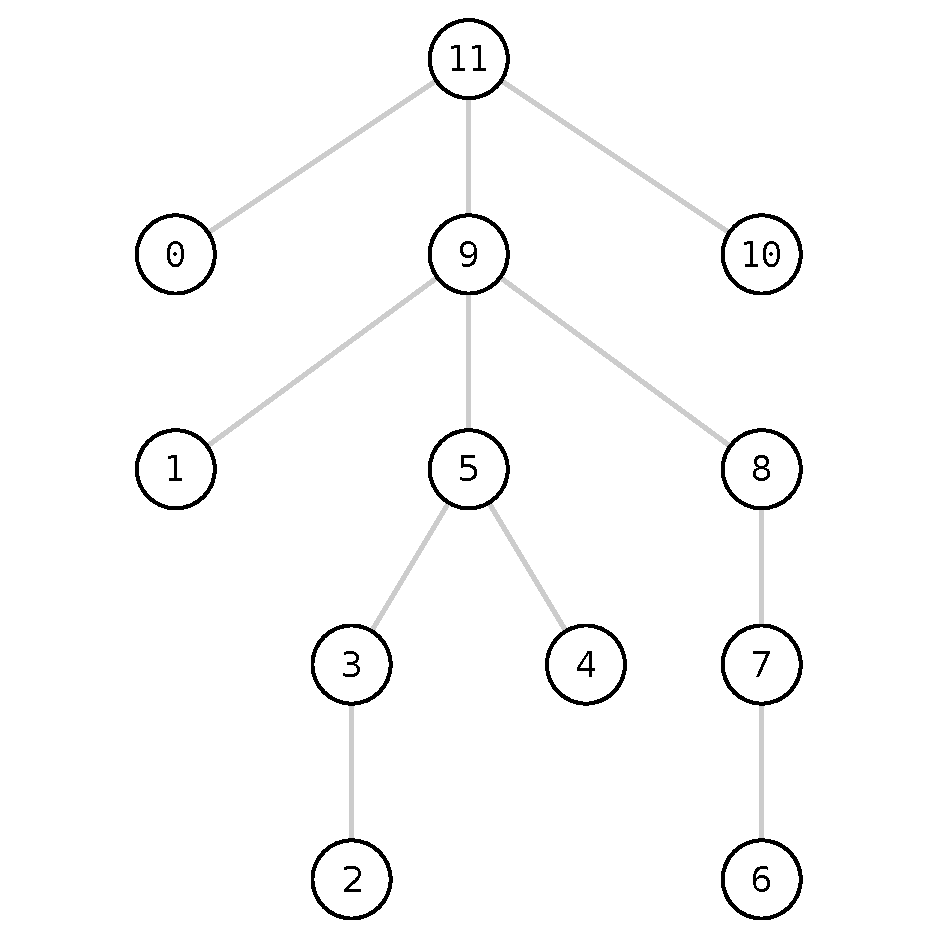
\includegraphics[width=0.28\textwidth]{python/lec02/dfs/dfs-0.pdf}\\[2pt]{\scriptsize Шаг 0}} &
\shortstack{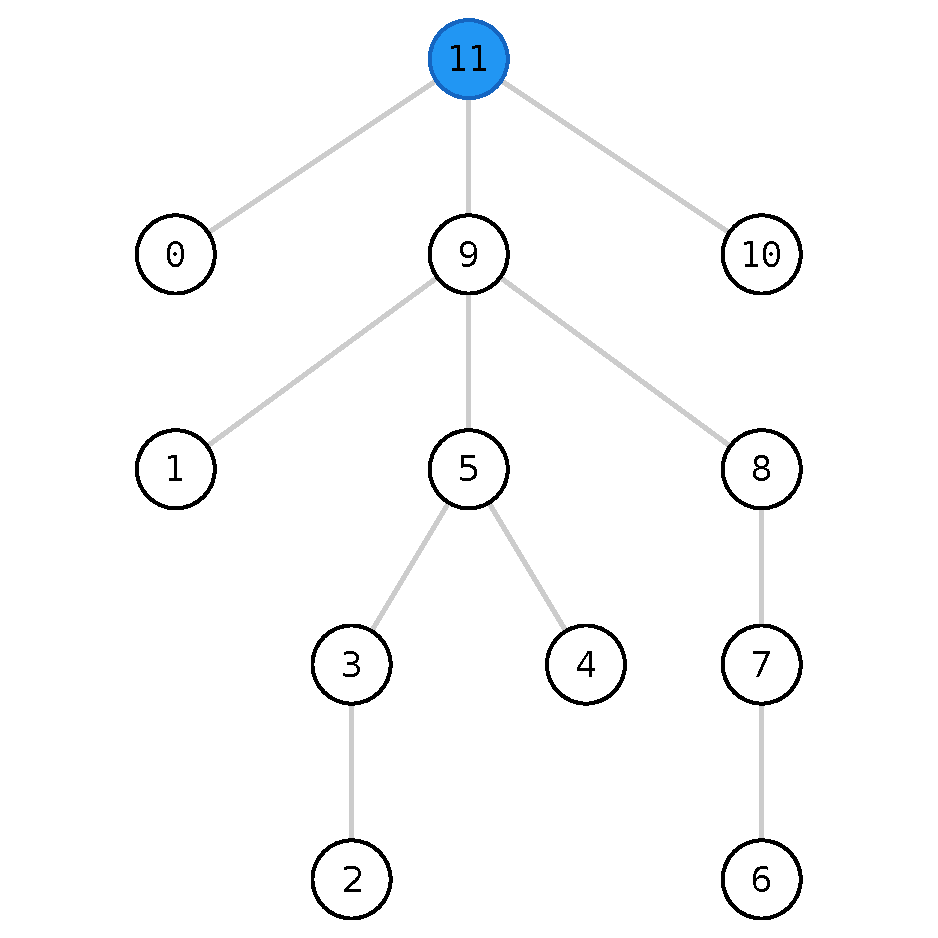
\includegraphics[width=0.28\textwidth]{python/lec02/dfs/dfs-1.pdf}\\[2pt]{\scriptsize Шаг 1}} &
\shortstack{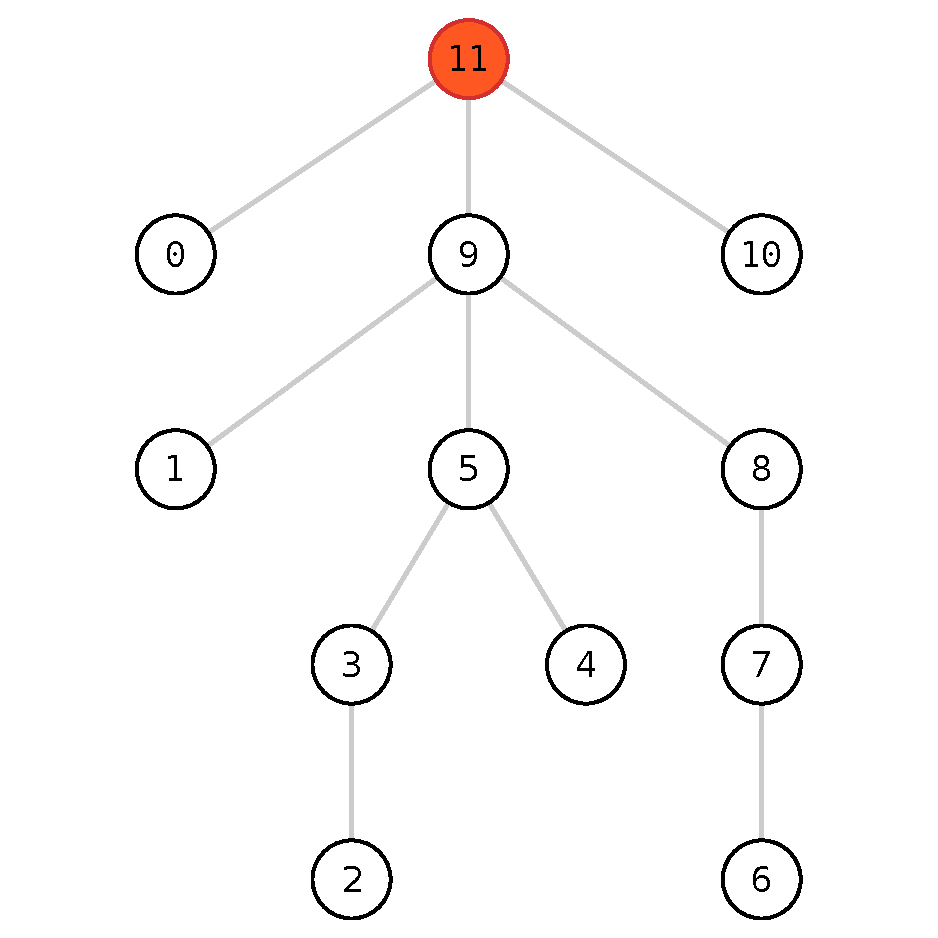
\includegraphics[width=0.28\textwidth]{python/lec02/dfs/dfs-2.pdf}\\[2pt]{\scriptsize Шаг 2}} \\
\end{tabular}\end{center}
\begin{center}\begin{tabular}{ccc}
\shortstack{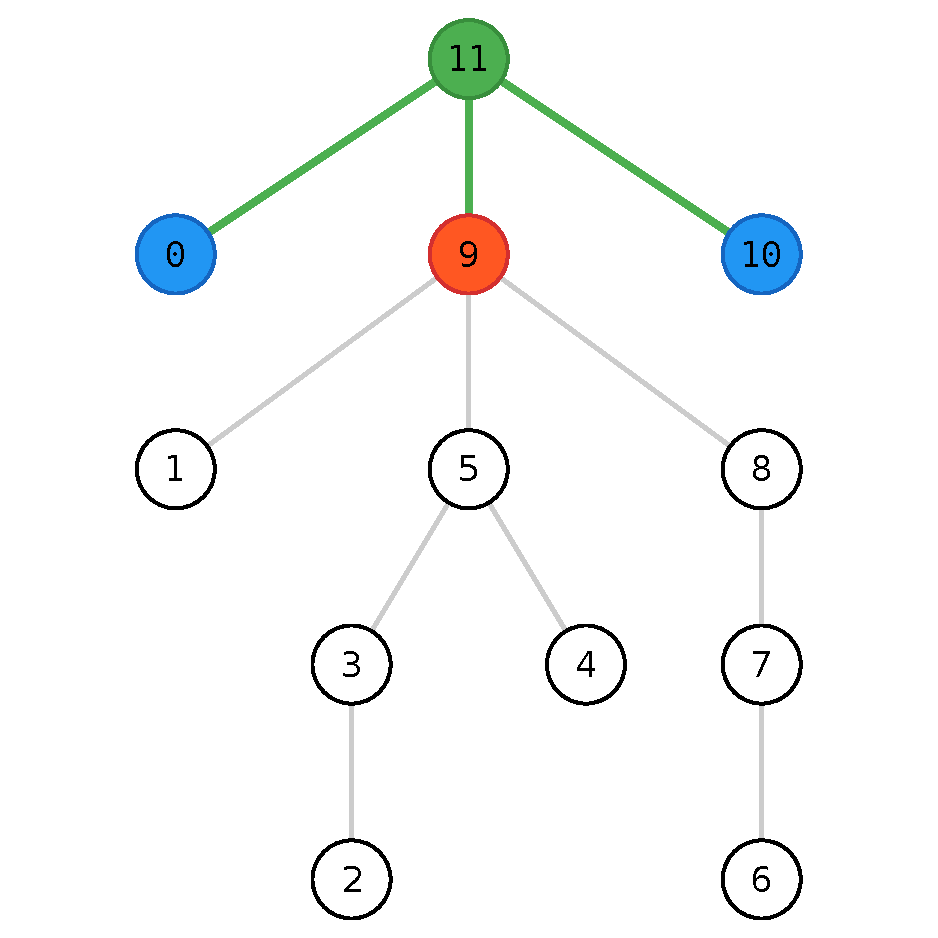
\includegraphics[width=0.28\textwidth]{python/lec02/dfs/dfs-3.pdf}\\[2pt]{\scriptsize Шаг 3}} &
\shortstack{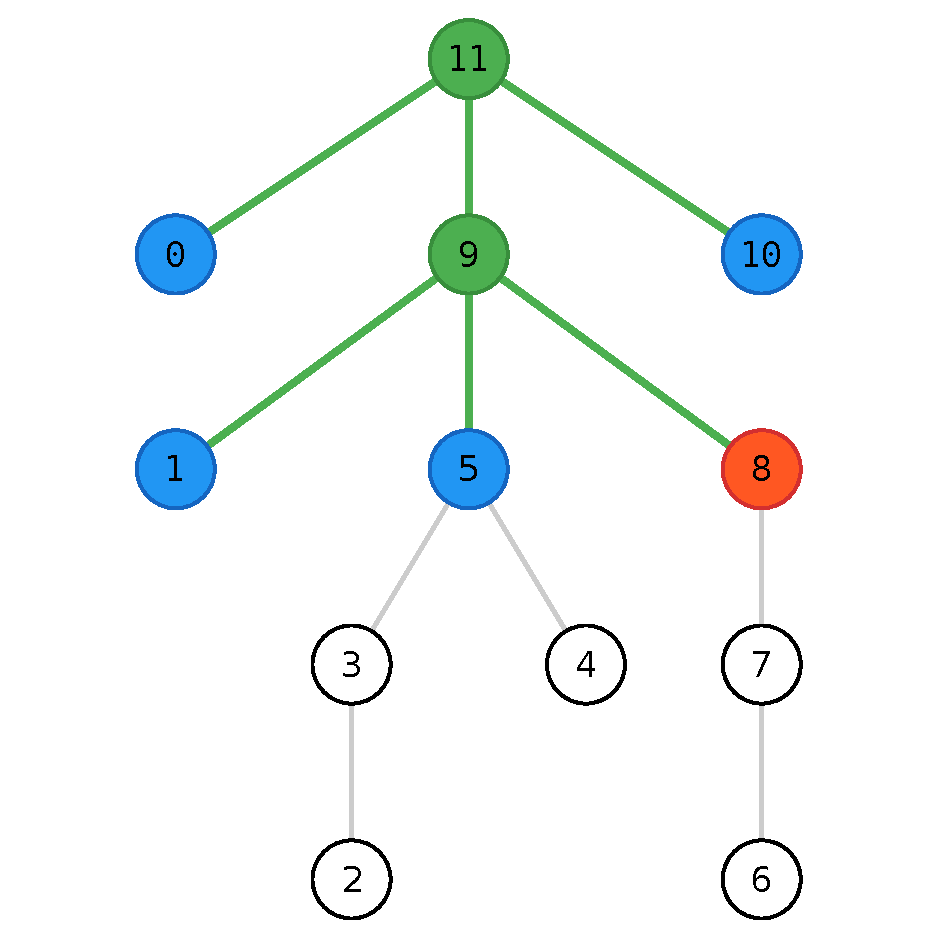
\includegraphics[width=0.28\textwidth]{python/lec02/dfs/dfs-4.pdf}\\[2pt]{\scriptsize Шаг 4}} &
\shortstack{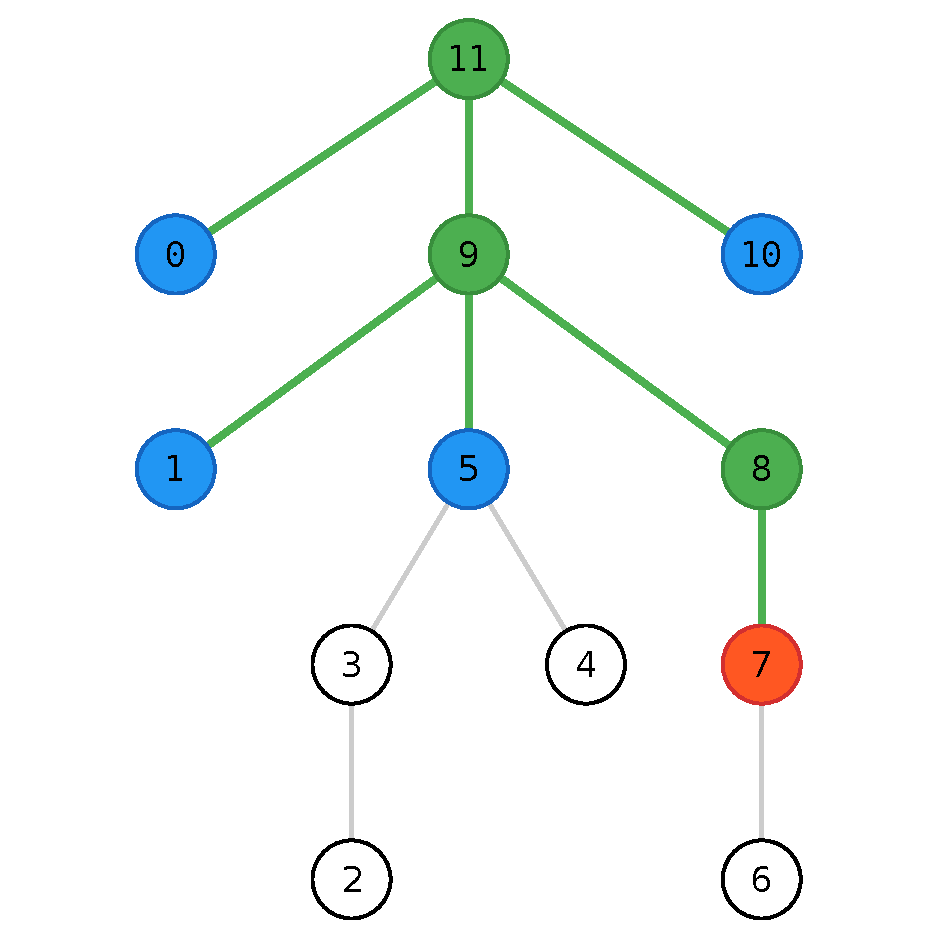
\includegraphics[width=0.28\textwidth]{python/lec02/dfs/dfs-5.pdf}\\[2pt]{\scriptsize Шаг 5}} \\
\end{tabular}\end{center}
\begin{center}\begin{tabular}{ccc}
\shortstack{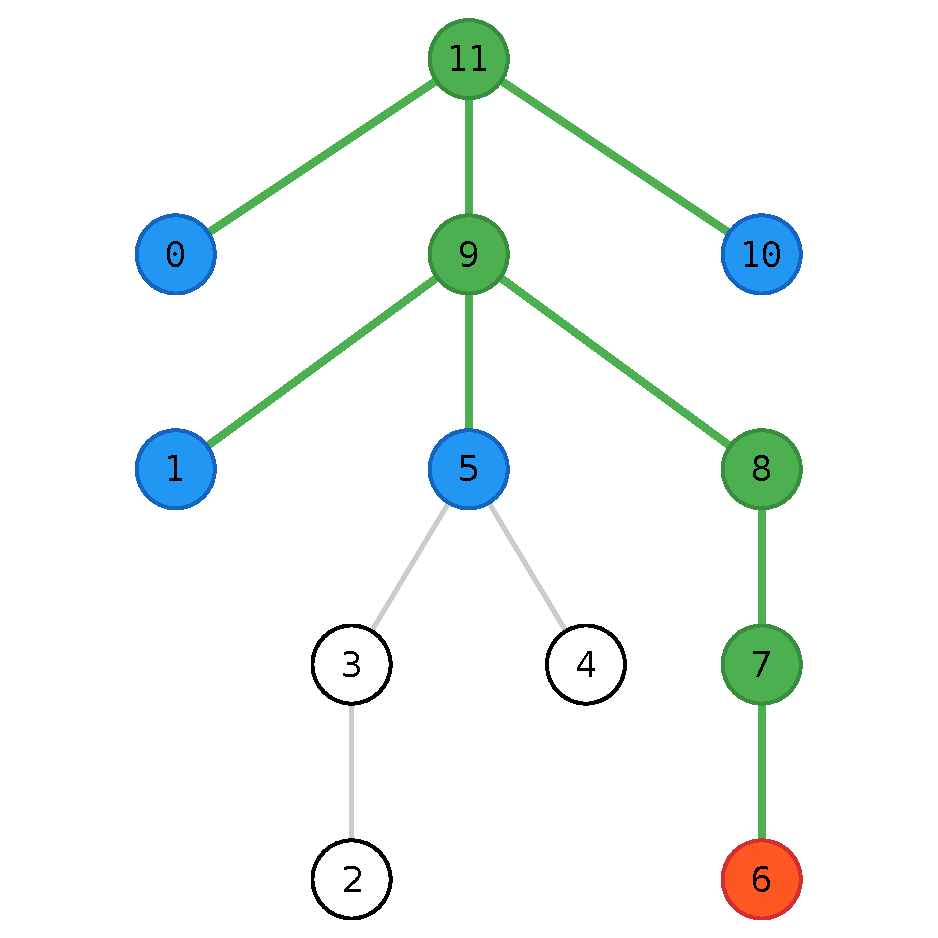
\includegraphics[width=0.28\textwidth]{python/lec02/dfs/dfs-6.pdf}\\[2pt]{\scriptsize Шаг 6}} &
\shortstack{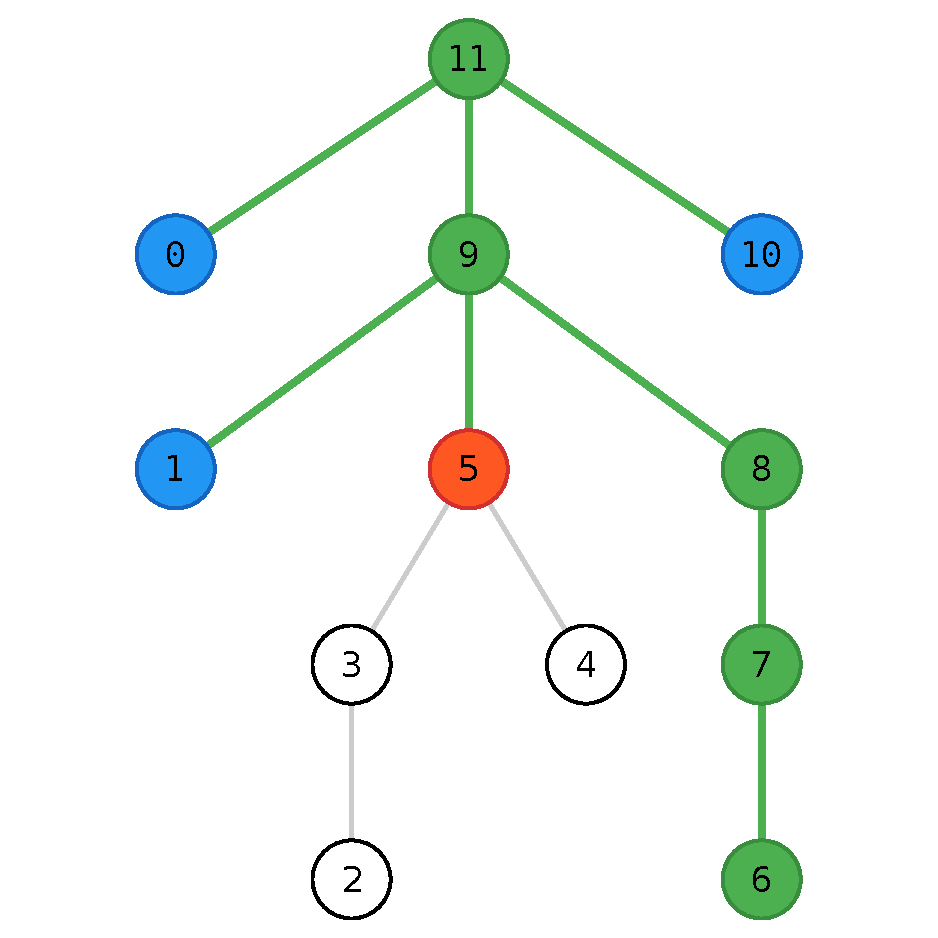
\includegraphics[width=0.28\textwidth]{python/lec02/dfs/dfs-7.pdf}\\[2pt]{\scriptsize Шаг 7}} &
\shortstack{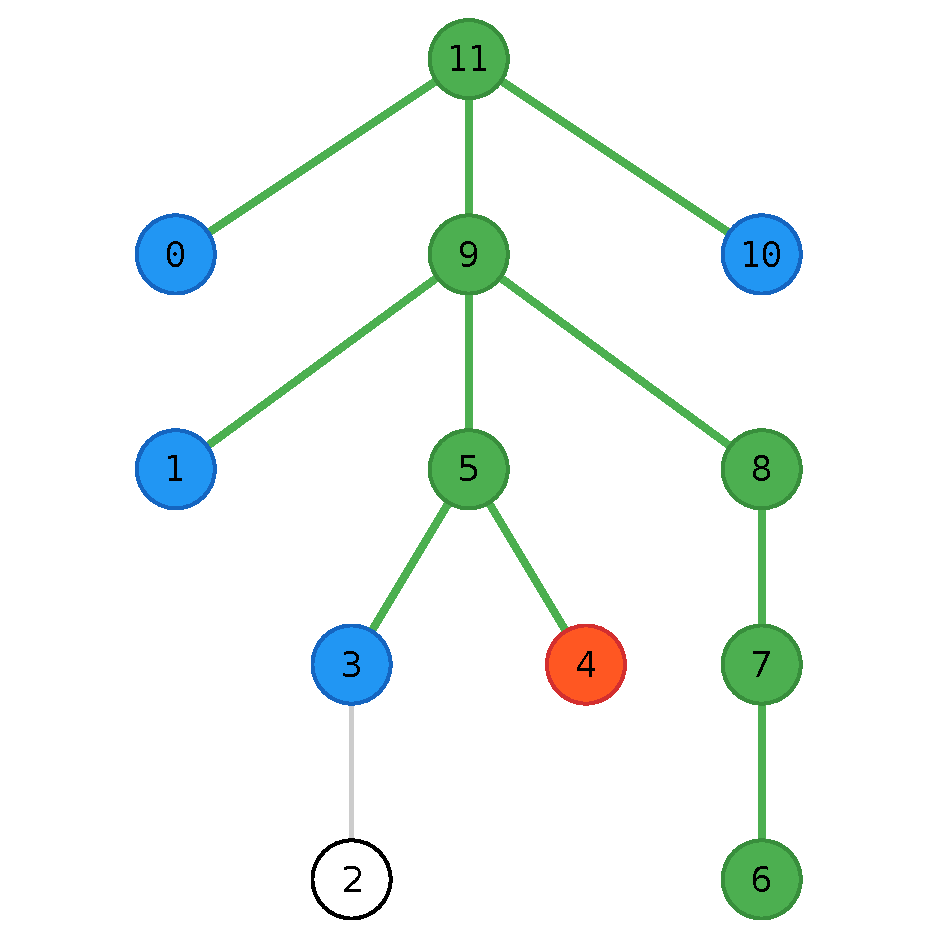
\includegraphics[width=0.28\textwidth]{python/lec02/dfs/dfs-8.pdf}\\[2pt]{\scriptsize Шаг 8}} \\
\end{tabular}\end{center}
\begin{center}\begin{tabular}{ccc}
\shortstack{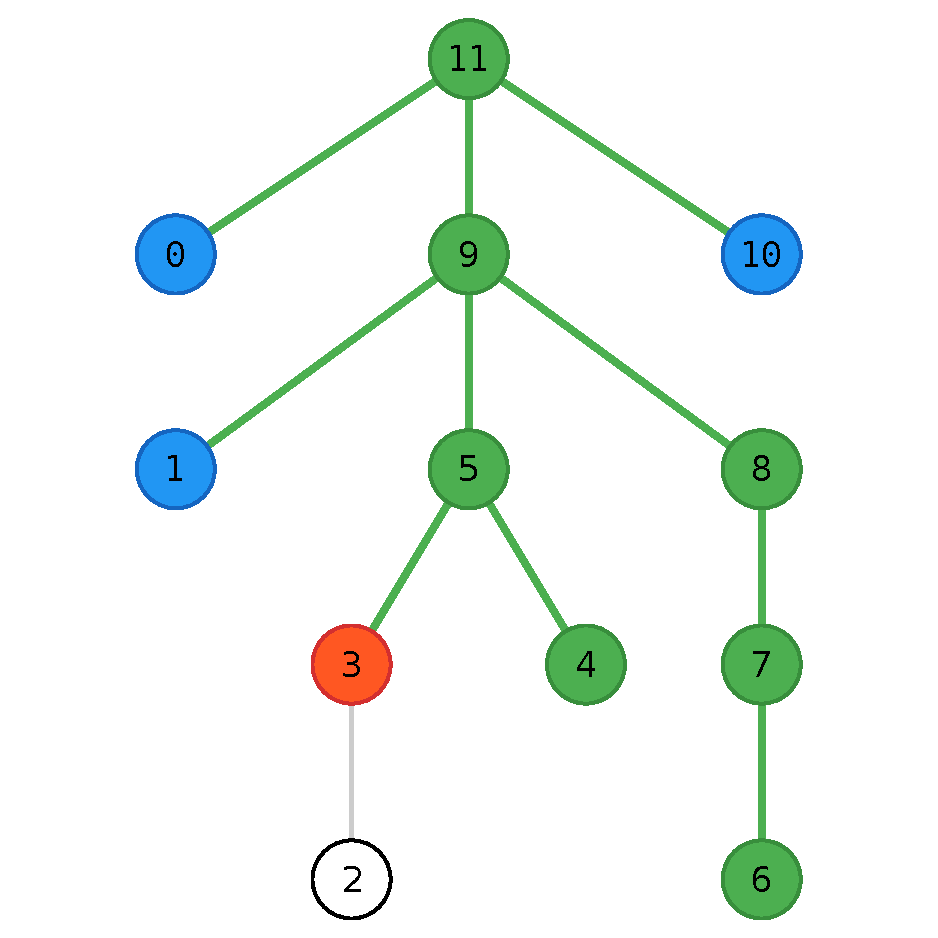
\includegraphics[width=0.28\textwidth]{python/lec02/dfs/dfs-9.pdf}\\[2pt]{\scriptsize Шаг 9}} &
\shortstack{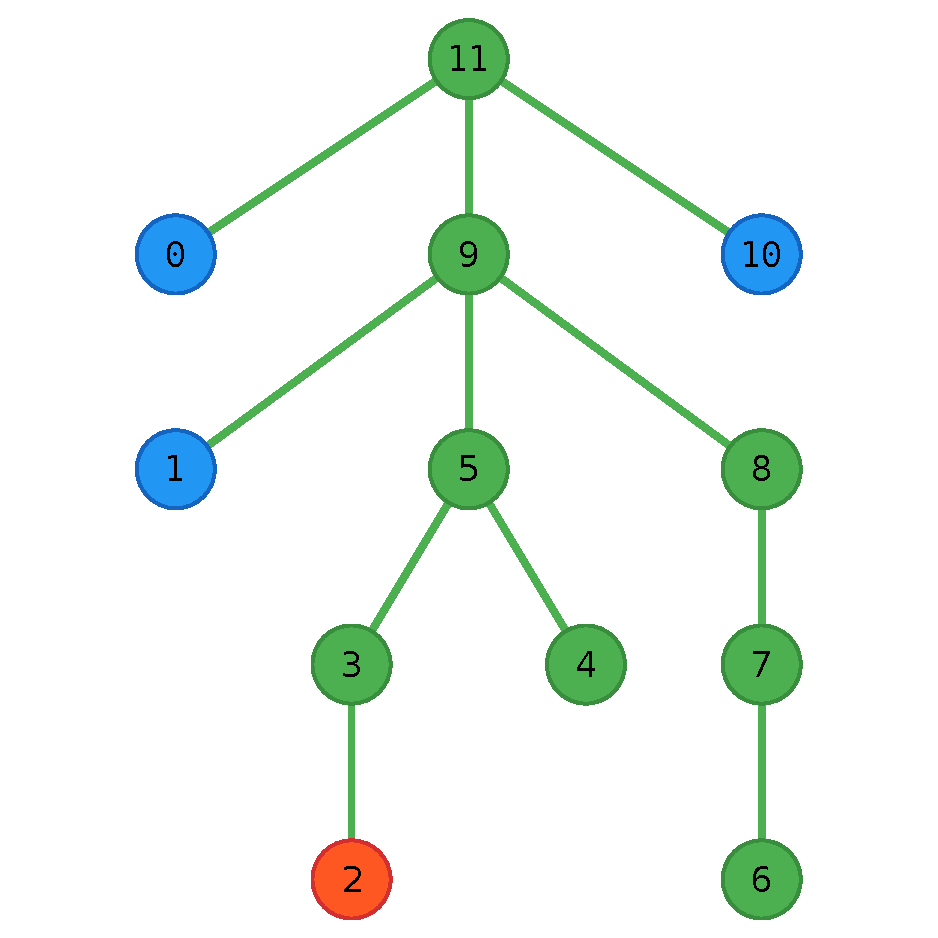
\includegraphics[width=0.28\textwidth]{python/lec02/dfs/dfs-10.pdf}\\[2pt]{\scriptsize Шаг 10}} &
\shortstack{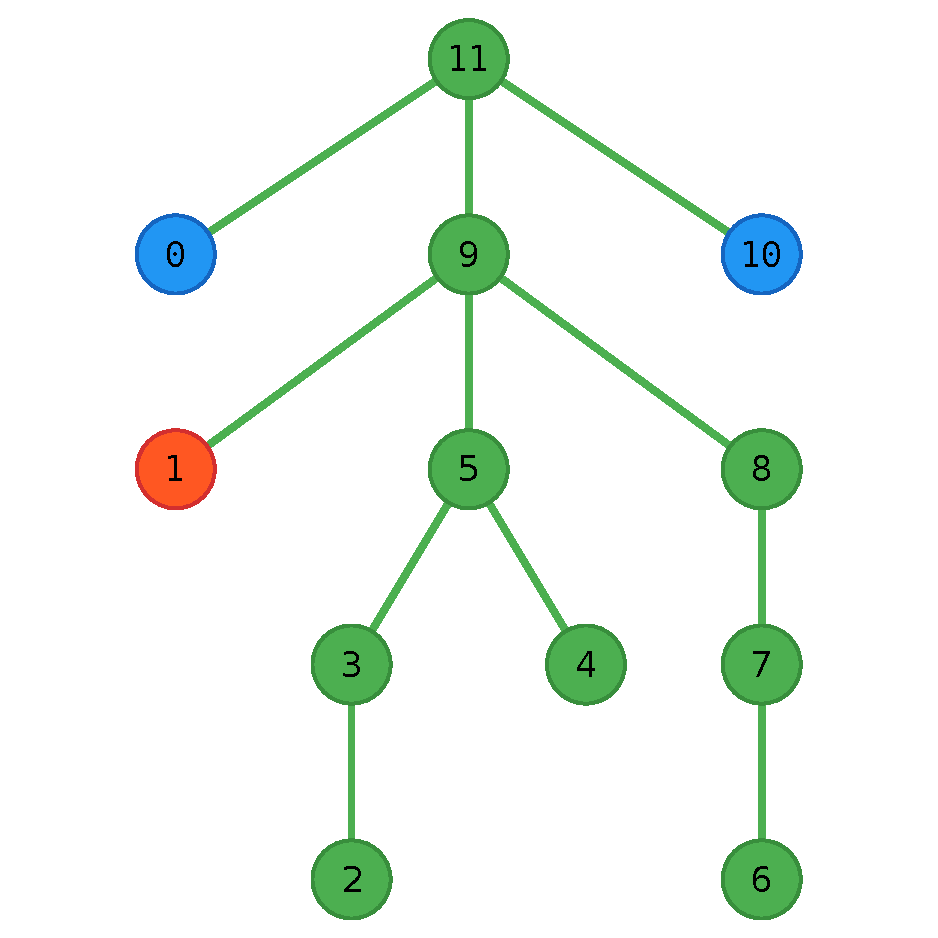
\includegraphics[width=0.28\textwidth]{python/lec02/dfs/dfs-11.pdf}\\[2pt]{\scriptsize Шаг 11}} \\
\end{tabular}\end{center}
\begin{center}\begin{tabular}{ccc}
\shortstack{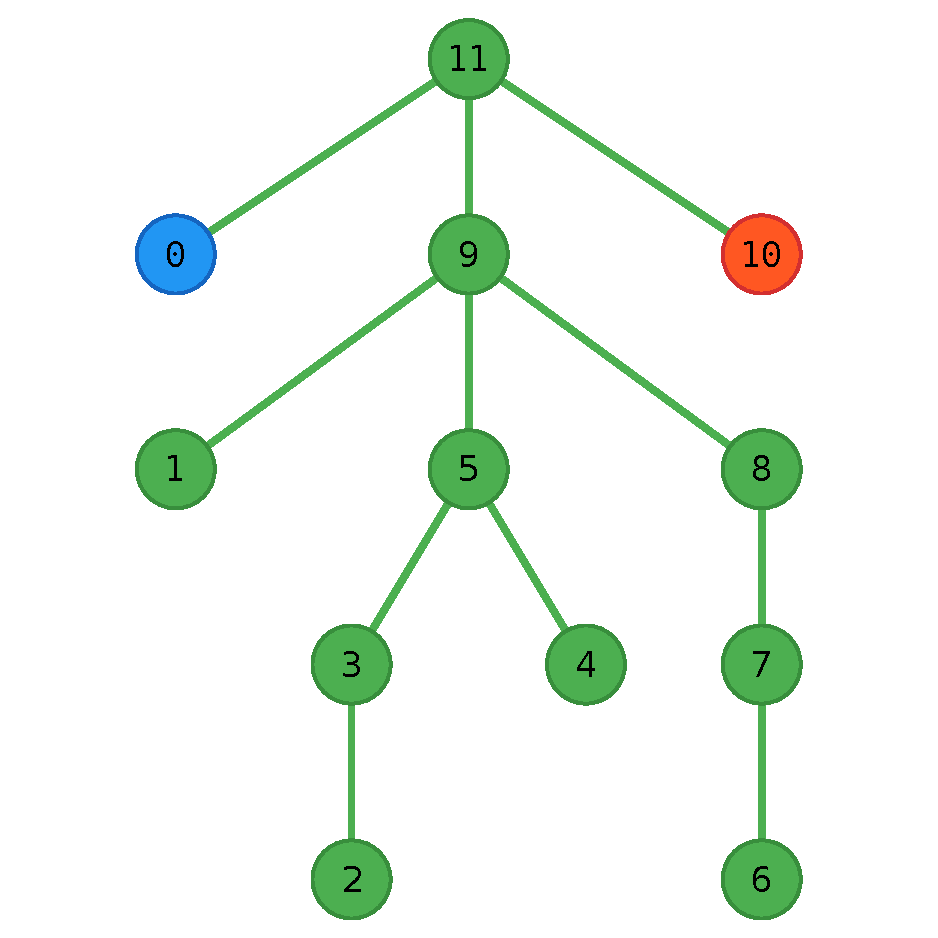
\includegraphics[width=0.28\textwidth]{python/lec02/dfs/dfs-12.pdf}\\[2pt]{\scriptsize Шаг 12}} &
\shortstack{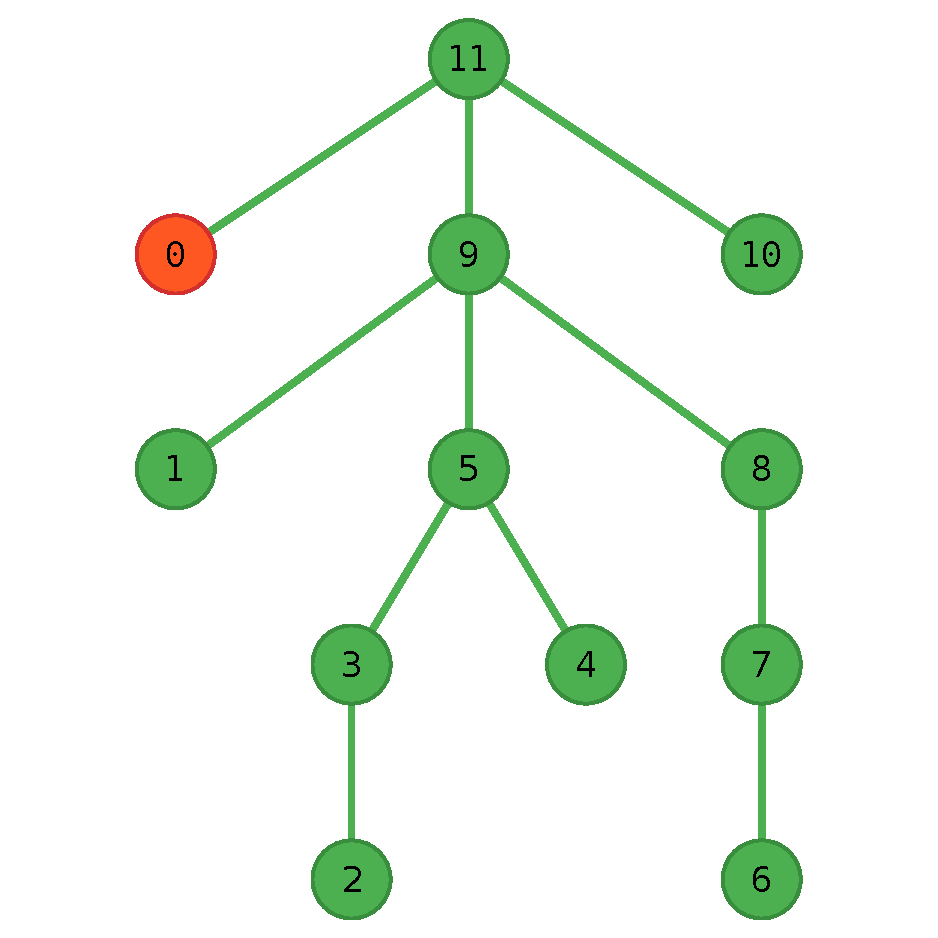
\includegraphics[width=0.28\textwidth]{python/lec02/dfs/dfs-13.pdf}\\[2pt]{\scriptsize Шаг 13}} &
\shortstack{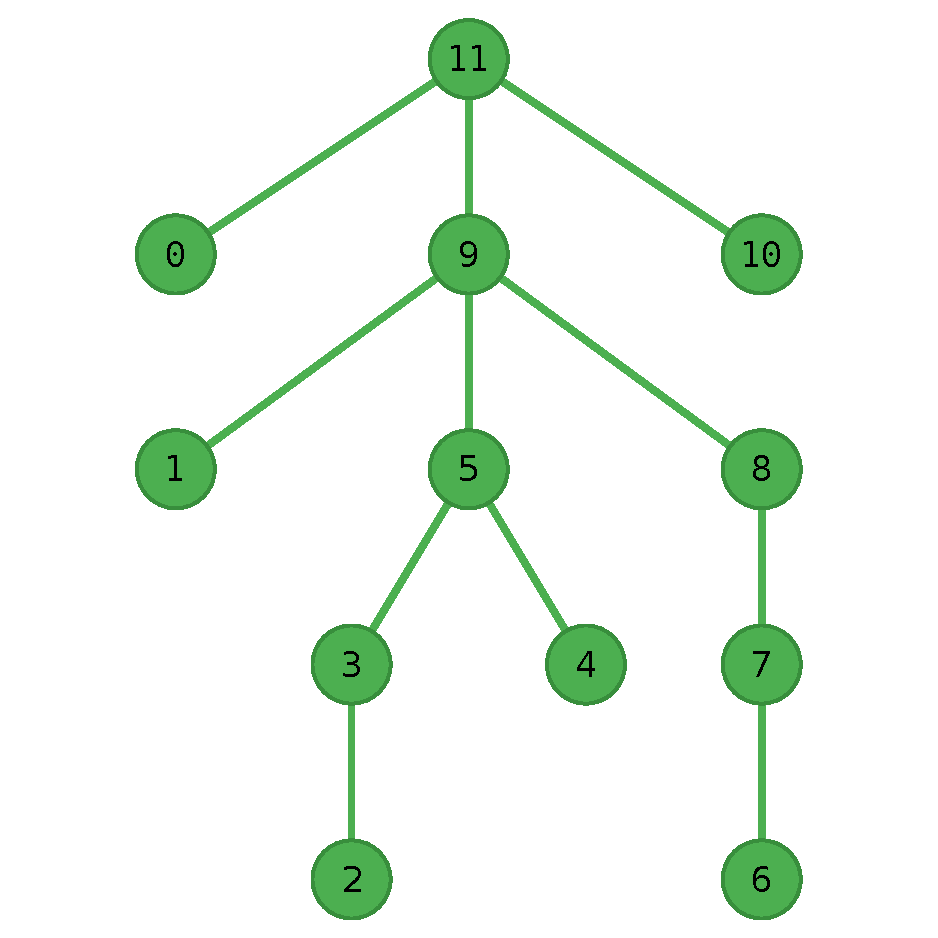
\includegraphics[width=0.28\textwidth]{python/lec02/dfs/dfs-14.pdf}\\[2pt]{\scriptsize Шаг 14}} \\
\end{tabular}\end{center}

\noindent\textbf{Пример работы BFS} (старт из $S$):

\begin{center}\begin{tabular}{ccc}
\shortstack{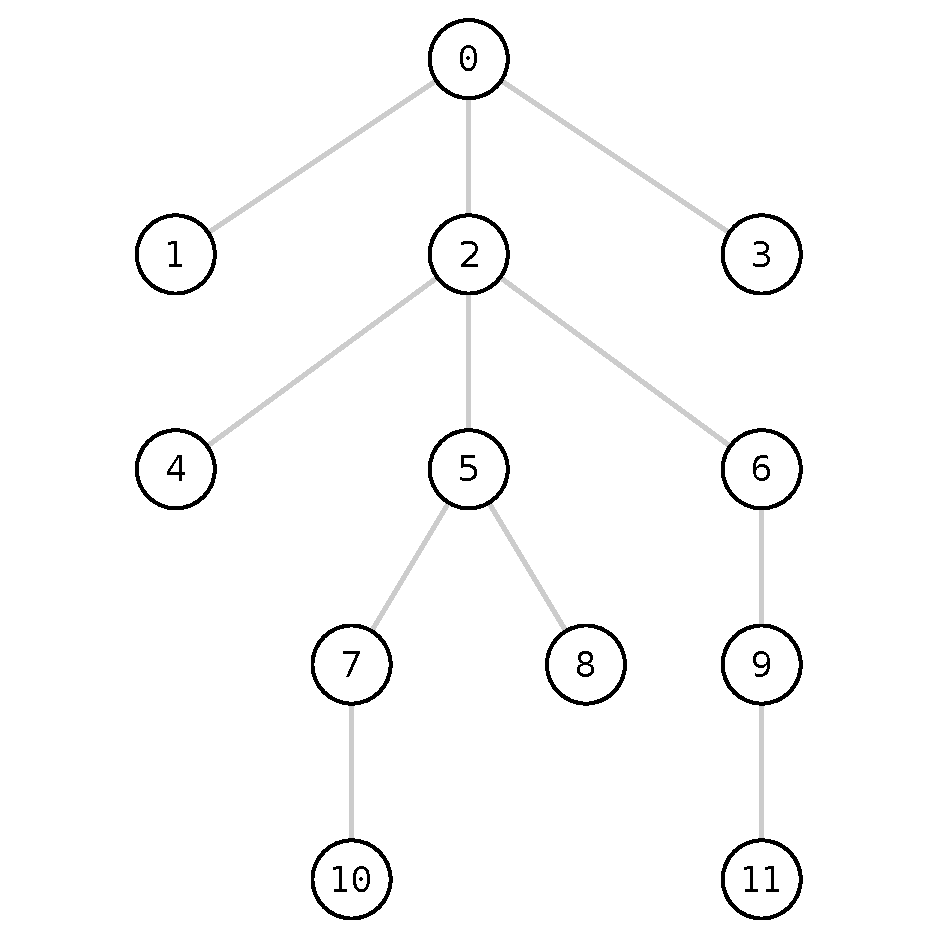
\includegraphics[width=0.28\textwidth]{python/lec02/bfs/bfs-0.pdf}\\[2pt]{\scriptsize Шаг 0}} &
\shortstack{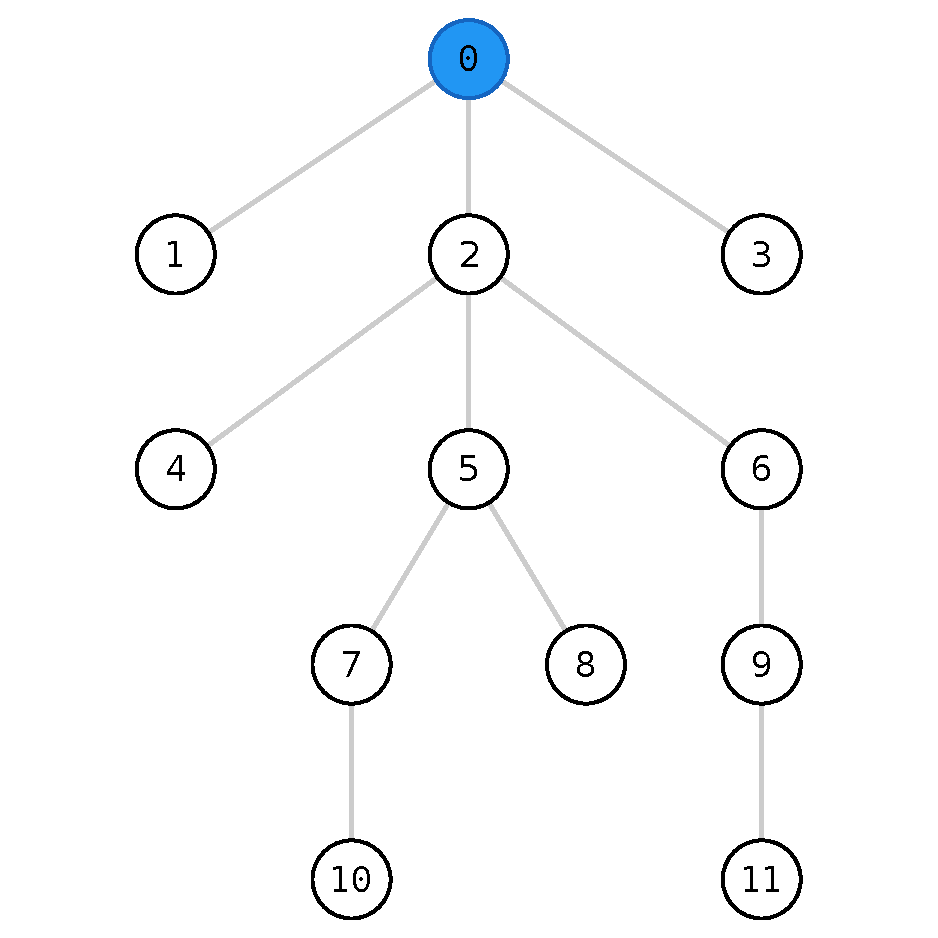
\includegraphics[width=0.28\textwidth]{python/lec02/bfs/bfs-1.pdf}\\[2pt]{\scriptsize Шаг 1}} &
\shortstack{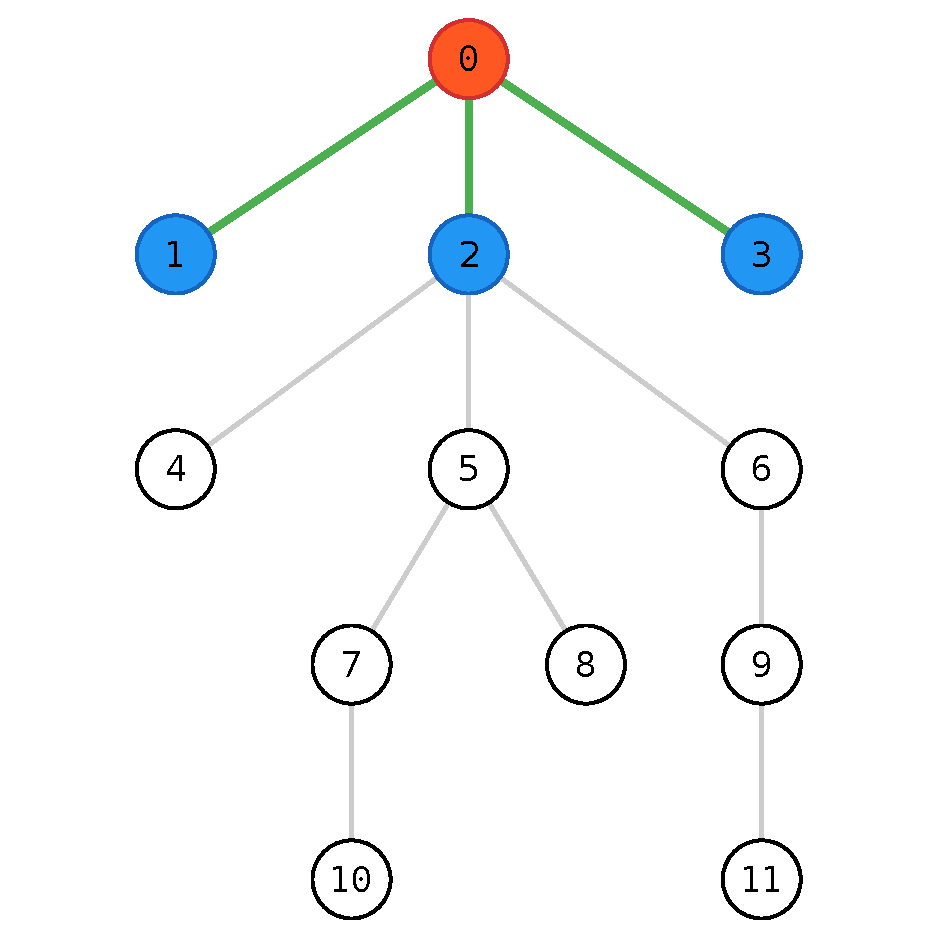
\includegraphics[width=0.28\textwidth]{python/lec02/bfs/bfs-2.pdf}\\[2pt]{\scriptsize Шаг 2}} \\
\end{tabular}\end{center}
\begin{center}\begin{tabular}{ccc}
\shortstack{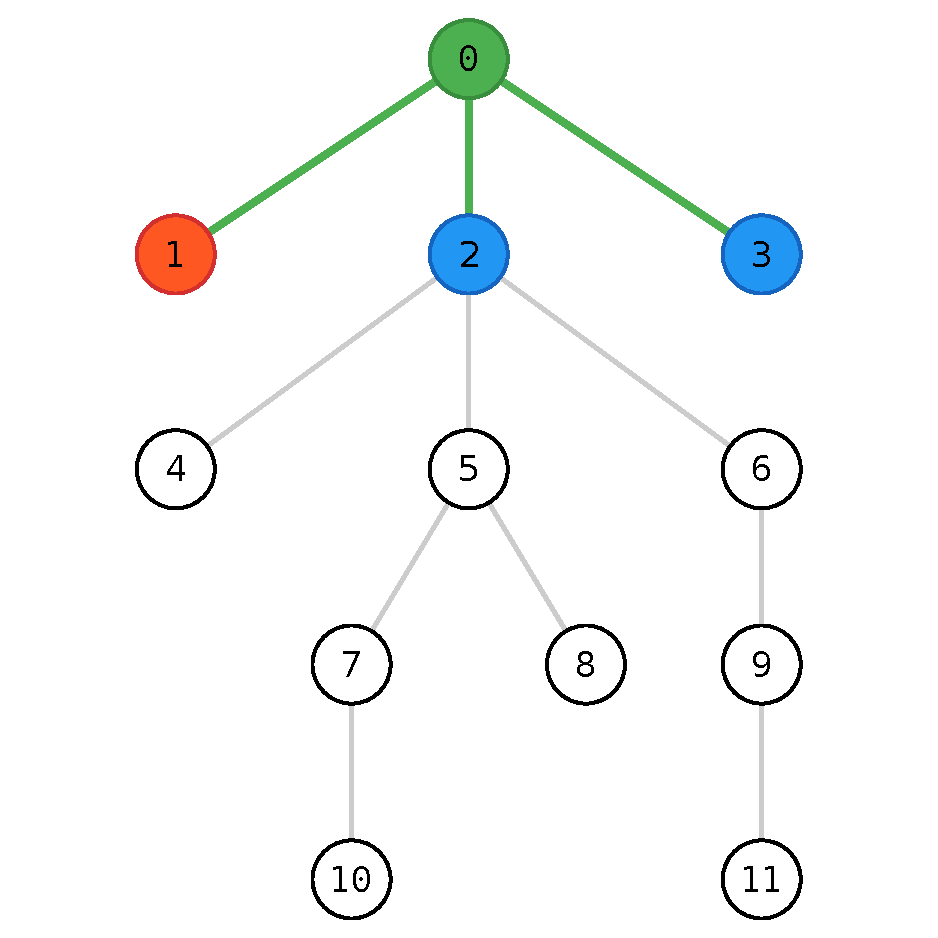
\includegraphics[width=0.28\textwidth]{python/lec02/bfs/bfs-3.pdf}\\[2pt]{\scriptsize Шаг 3}} &
\shortstack{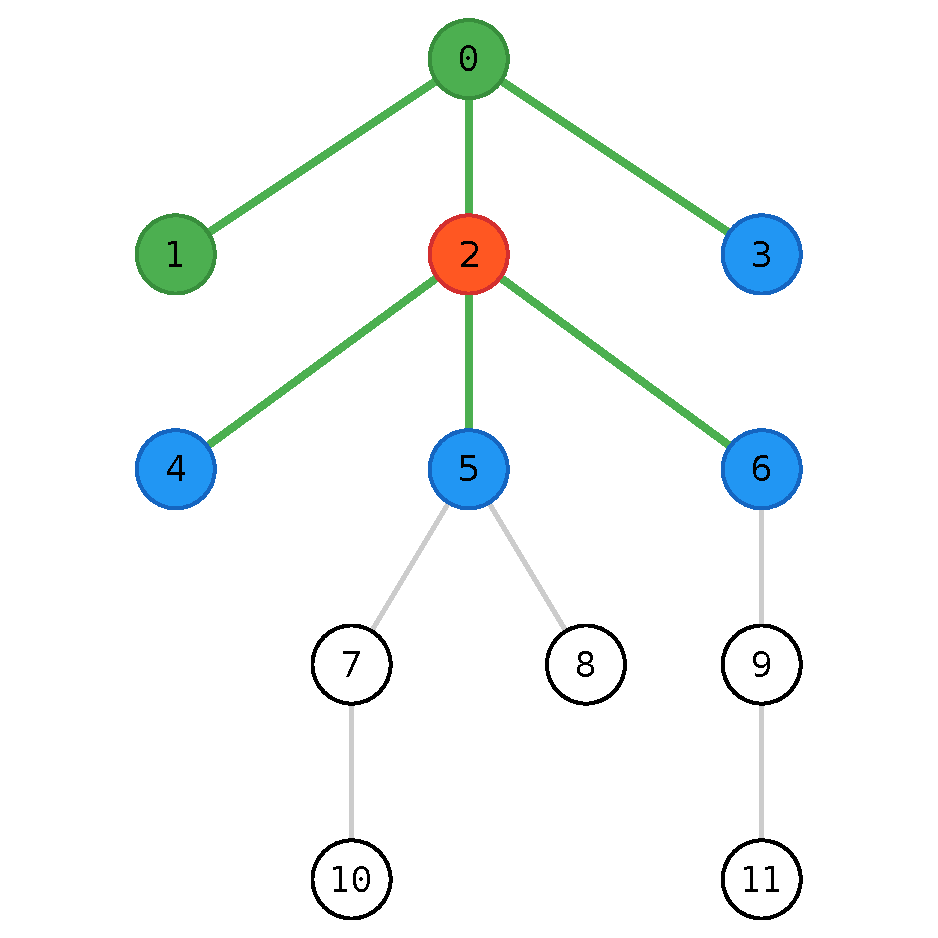
\includegraphics[width=0.28\textwidth]{python/lec02/bfs/bfs-4.pdf}\\[2pt]{\scriptsize Шаг 4}} &
\shortstack{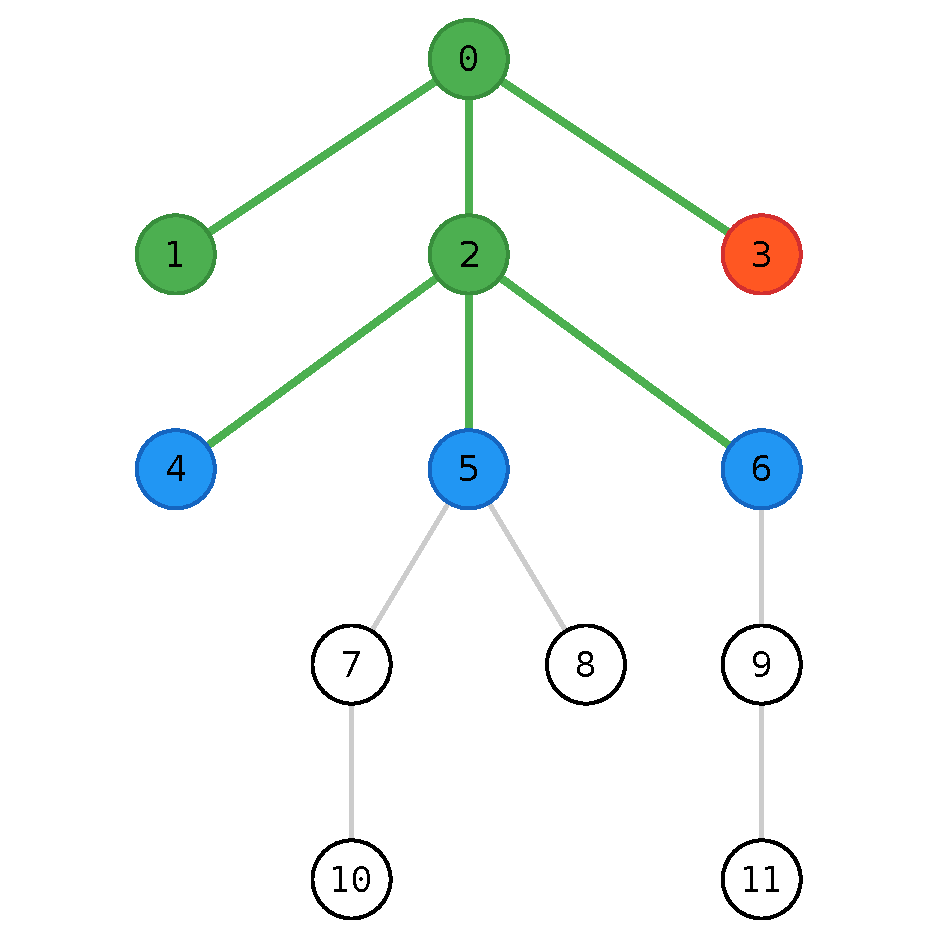
\includegraphics[width=0.28\textwidth]{python/lec02/bfs/bfs-5.pdf}\\[2pt]{\scriptsize Шаг 5}} \\
\end{tabular}\end{center}
\begin{center}\begin{tabular}{ccc}
\shortstack{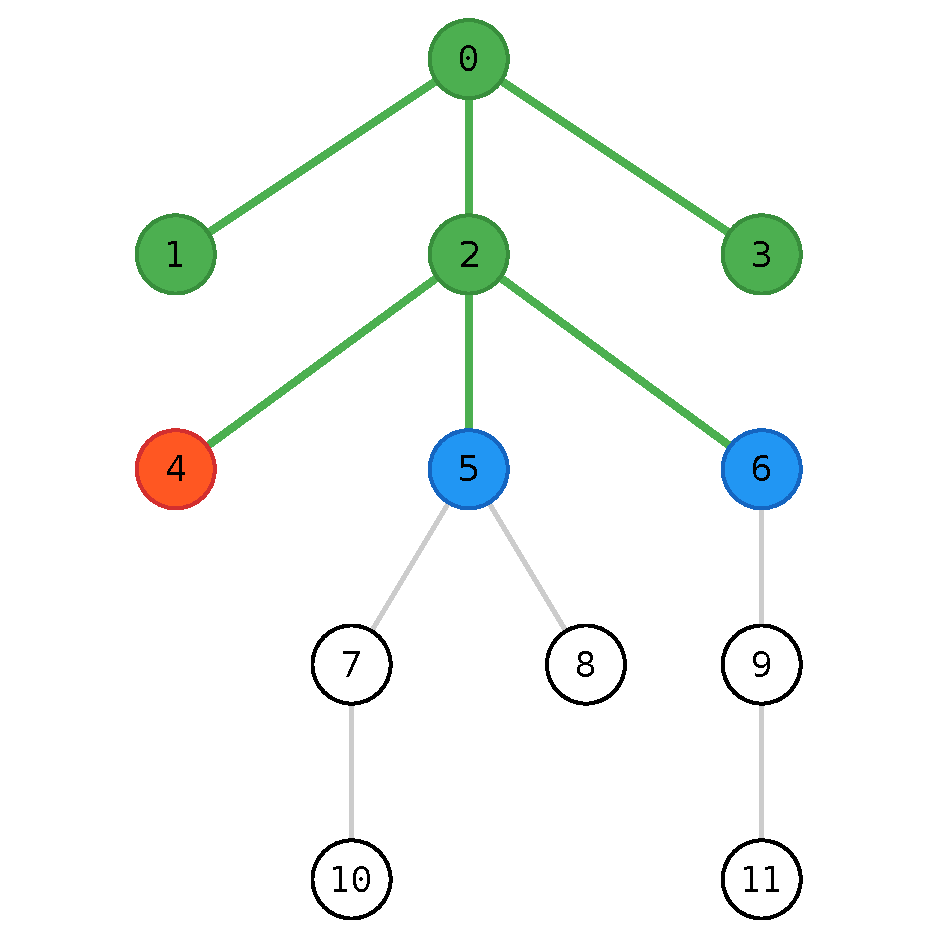
\includegraphics[width=0.28\textwidth]{python/lec02/bfs/bfs-6.pdf}\\[2pt]{\scriptsize Шаг 6}} &
\shortstack{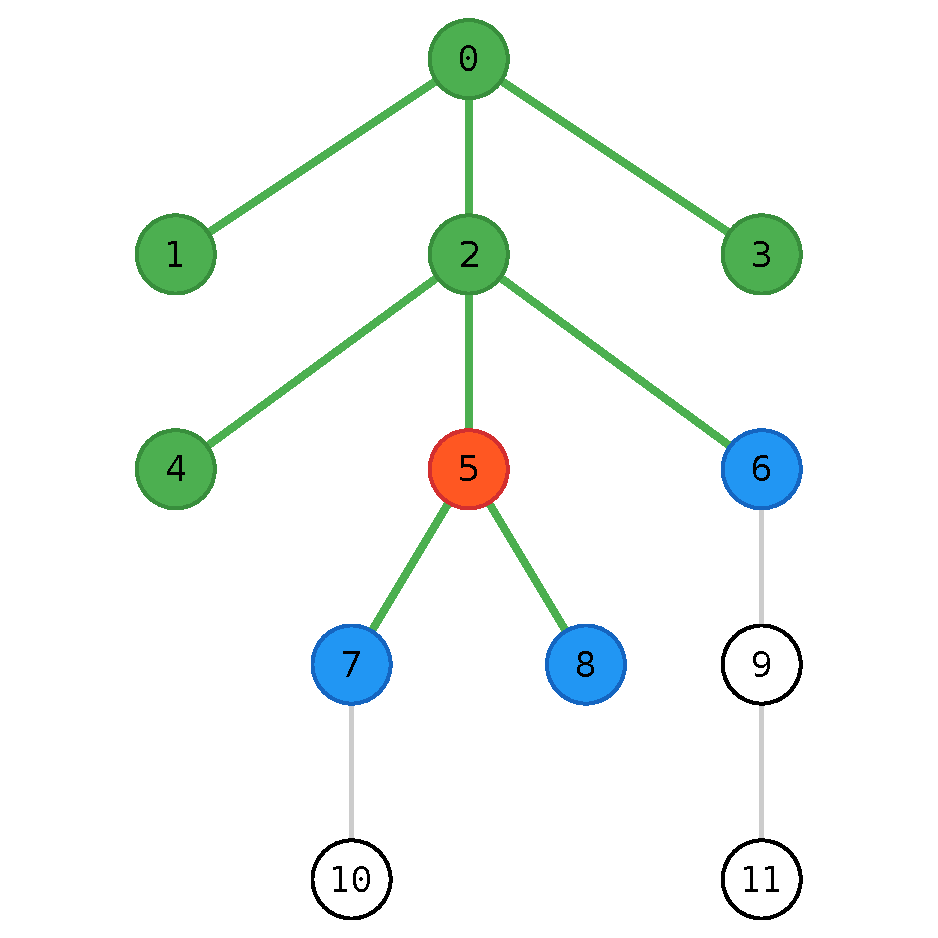
\includegraphics[width=0.28\textwidth]{python/lec02/bfs/bfs-7.pdf}\\[2pt]{\scriptsize Шаг 7}} &
\shortstack{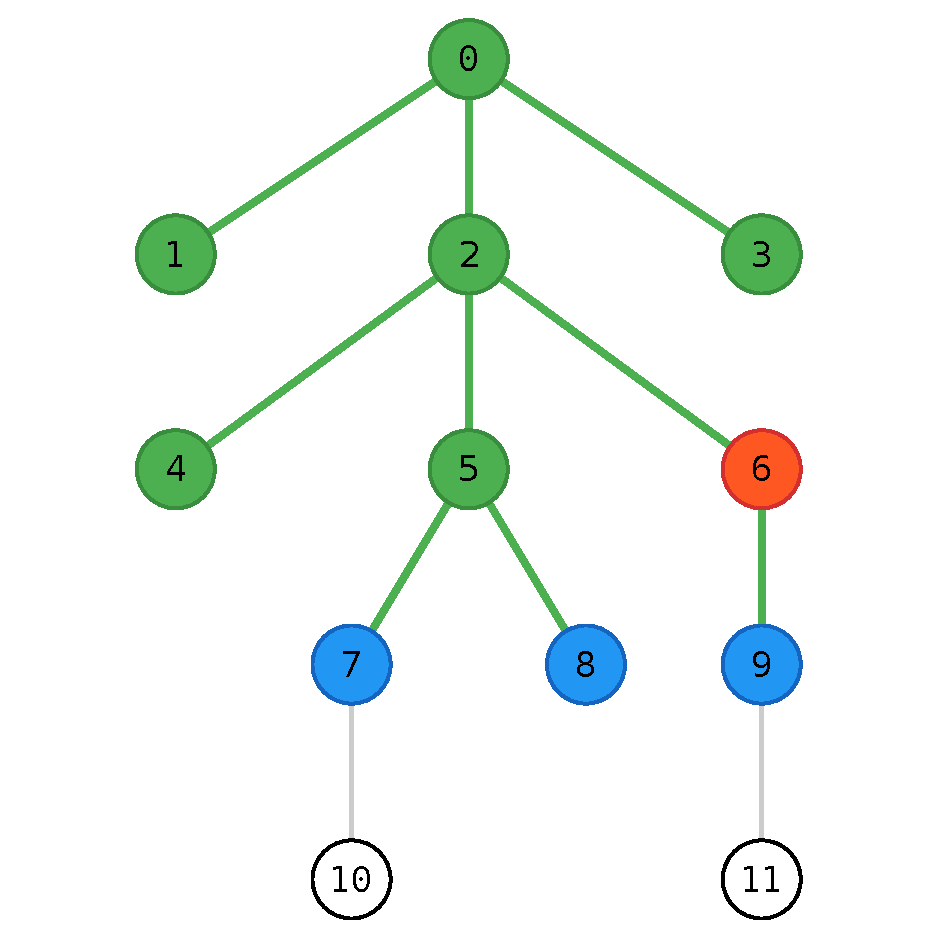
\includegraphics[width=0.28\textwidth]{python/lec02/bfs/bfs-8.pdf}\\[2pt]{\scriptsize Шаг 8}} \\
\end{tabular}\end{center}
\begin{center}\begin{tabular}{ccc}
\shortstack{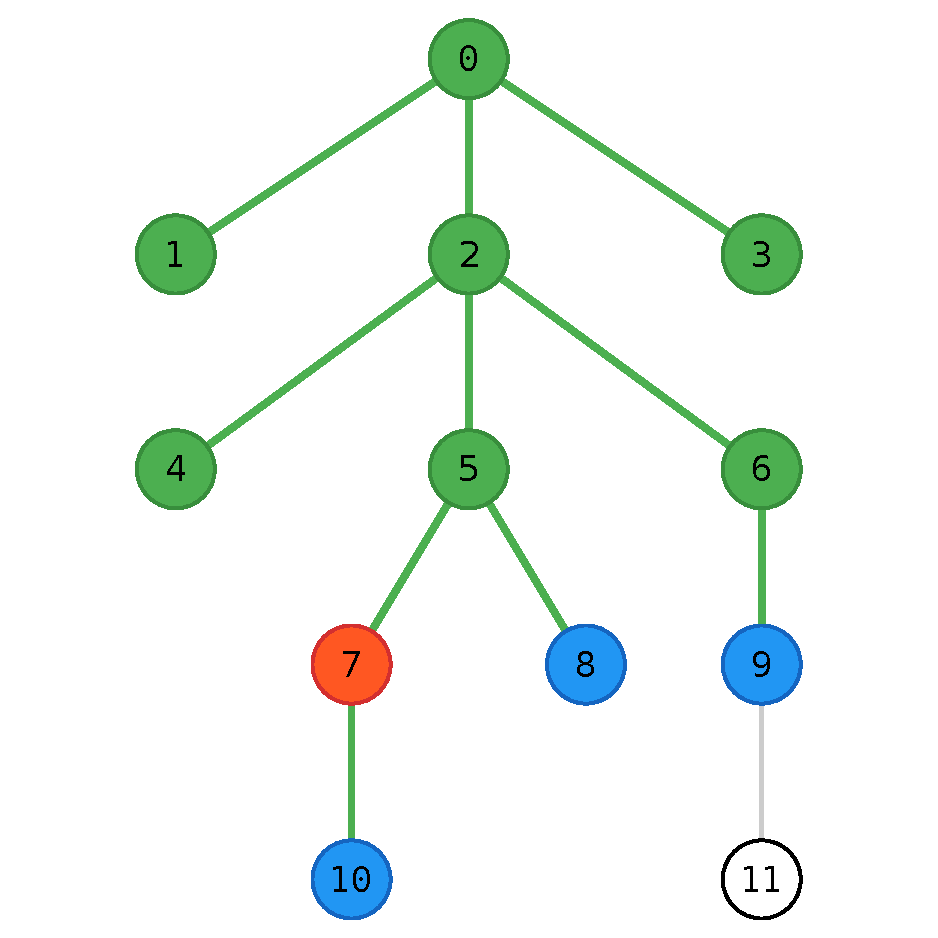
\includegraphics[width=0.28\textwidth]{python/lec02/bfs/bfs-9.pdf}\\[2pt]{\scriptsize Шаг 9}} &
\shortstack{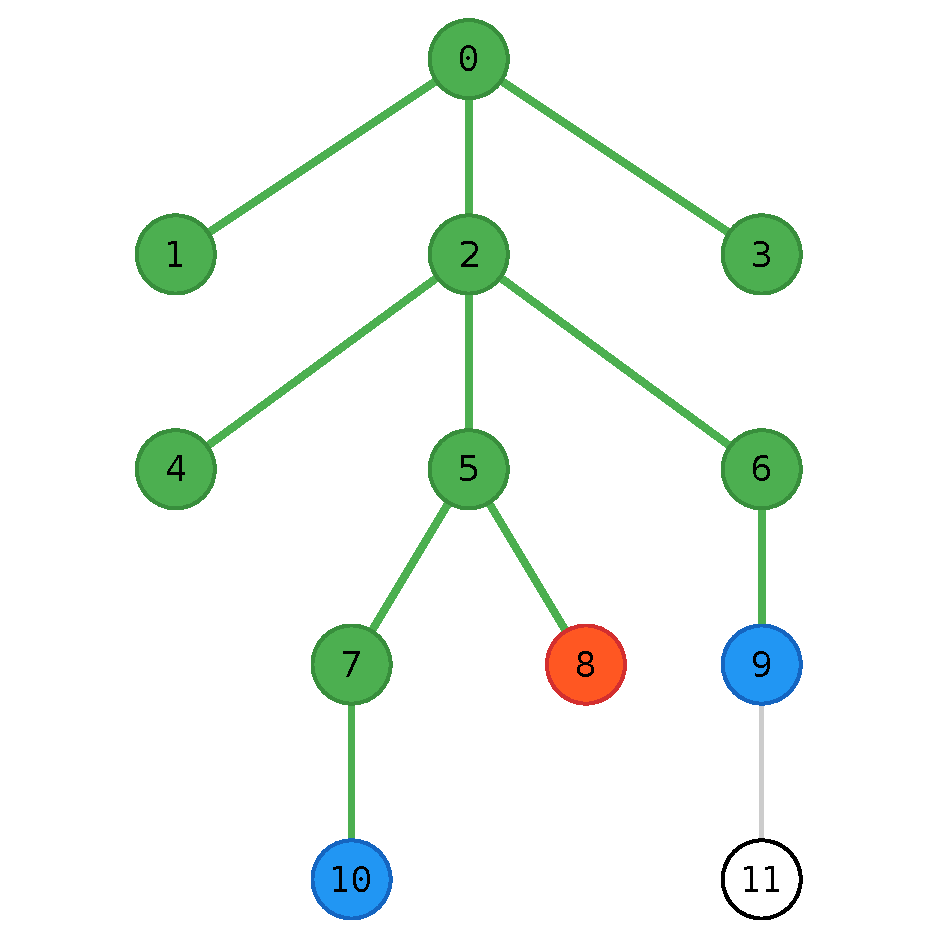
\includegraphics[width=0.28\textwidth]{python/lec02/bfs/bfs-10.pdf}\\[2pt]{\scriptsize Шаг 10}} &
\shortstack{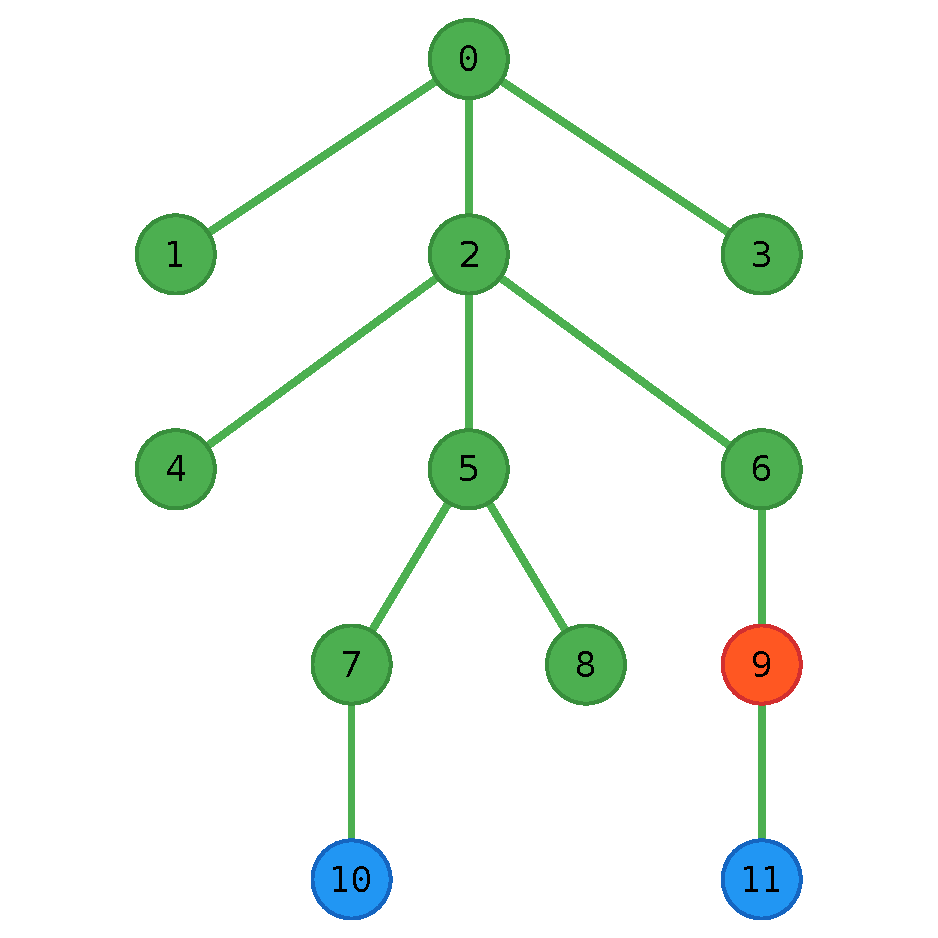
\includegraphics[width=0.28\textwidth]{python/lec02/bfs/bfs-11.pdf}\\[2pt]{\scriptsize Шаг 11}} \\
\end{tabular}\end{center}
\begin{center}\begin{tabular}{ccc}
\shortstack{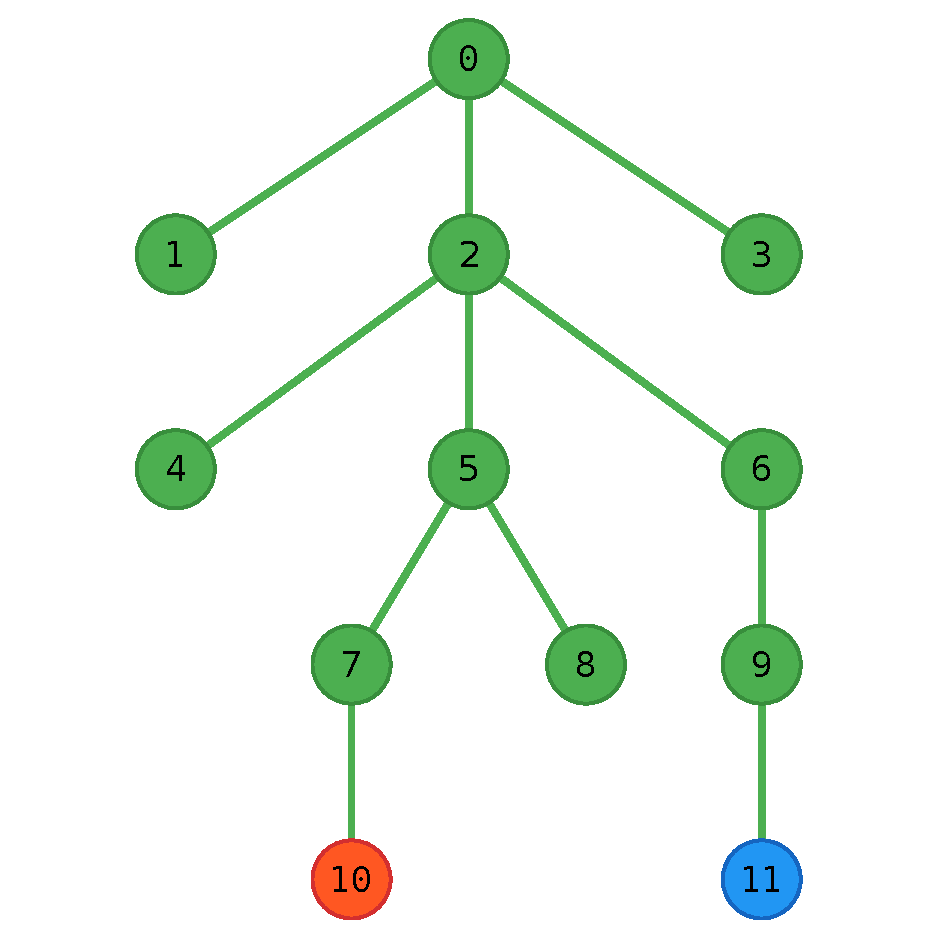
\includegraphics[width=0.28\textwidth]{python/lec02/bfs/bfs-12.pdf}\\[2pt]{\scriptsize Шаг 12}} &
\shortstack{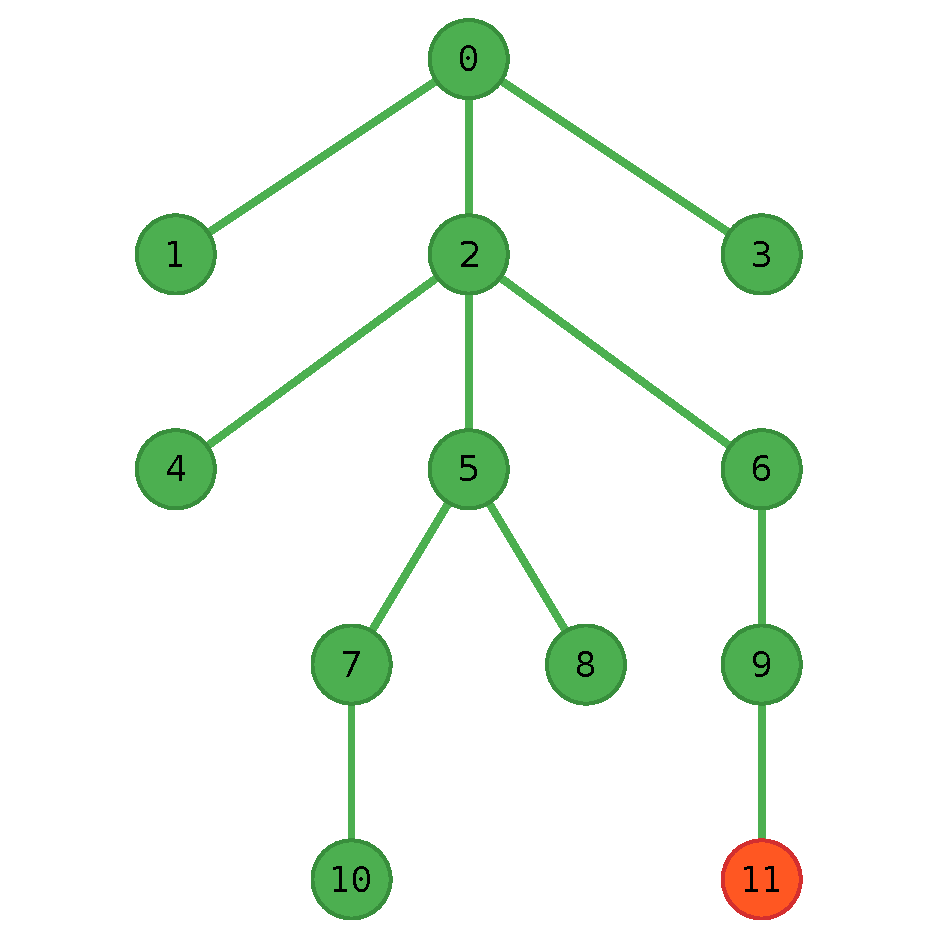
\includegraphics[width=0.28\textwidth]{python/lec02/bfs/bfs-13.pdf}\\[2pt]{\scriptsize Шаг 13}} &
\shortstack{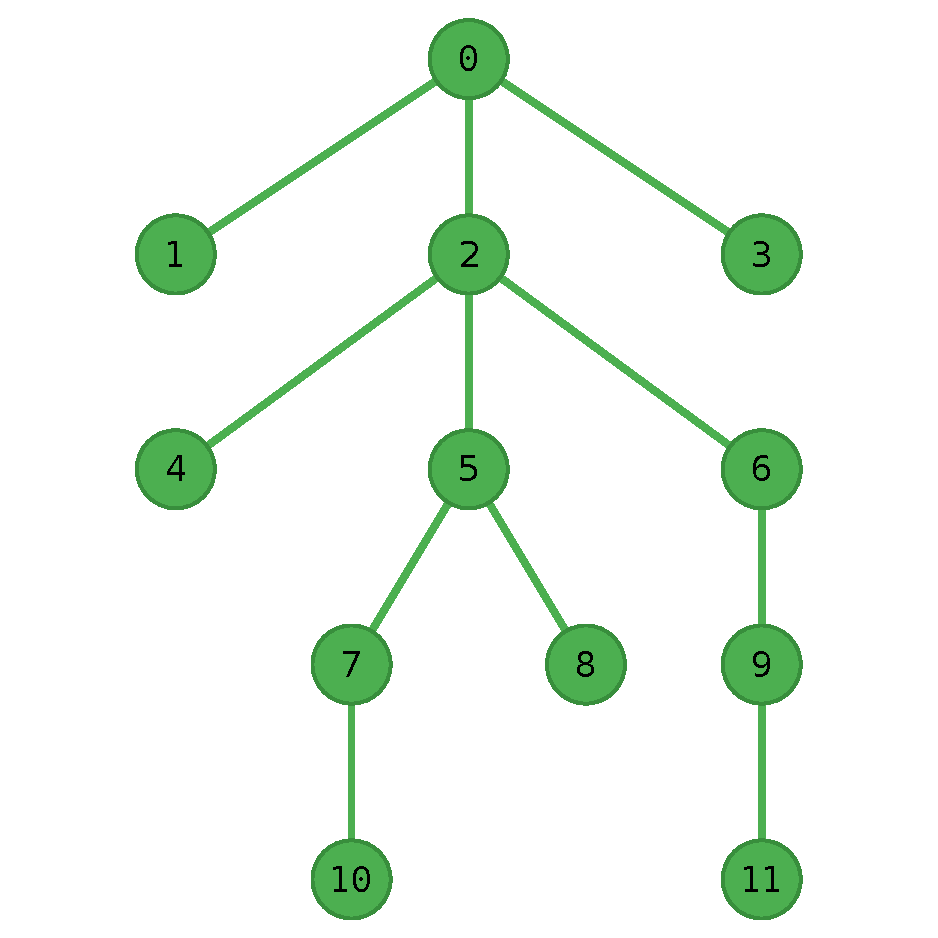
\includegraphics[width=0.28\textwidth]{python/lec02/bfs/bfs-14.pdf}\\[2pt]{\scriptsize Шаг 14}} \\
\end{tabular}\end{center}

\end{algo}


\bigskip
\begin{algo}{Топологическая сортировка (Topsort)}{topsort}
\textit{Дано:} ориентированный граф без циклов, задающий частичный порядок.
\textit{Построить:} линейный порядок, согласованный с исходным.

\medskip
\textbf{Шаг I.} Серия поисков в глубину (DFS). Когда вершина становится
<<тупиковой>> (все её исходящие рёбра уже обработаны), она кладётся в стек.

\textbf{Шаг II.} Нумеруем вершины по стеку \emph{снизу вверх}: самая нижняя
вершина стека получает номер~1, верхняя --- номер $n$. После этого
дорисовываем рефлексивные петли и недостающие рёбра: из каждой вершины
с \emph{бóльшим} номером --- во все вершины с \emph{меньшим} номером.

Результат --- граф, задающий отношение \textbf{линейного порядка}.

\medskip
\noindent\textbf{Работа алгоритма по шагам.} Исходный граф:

\begin{center}
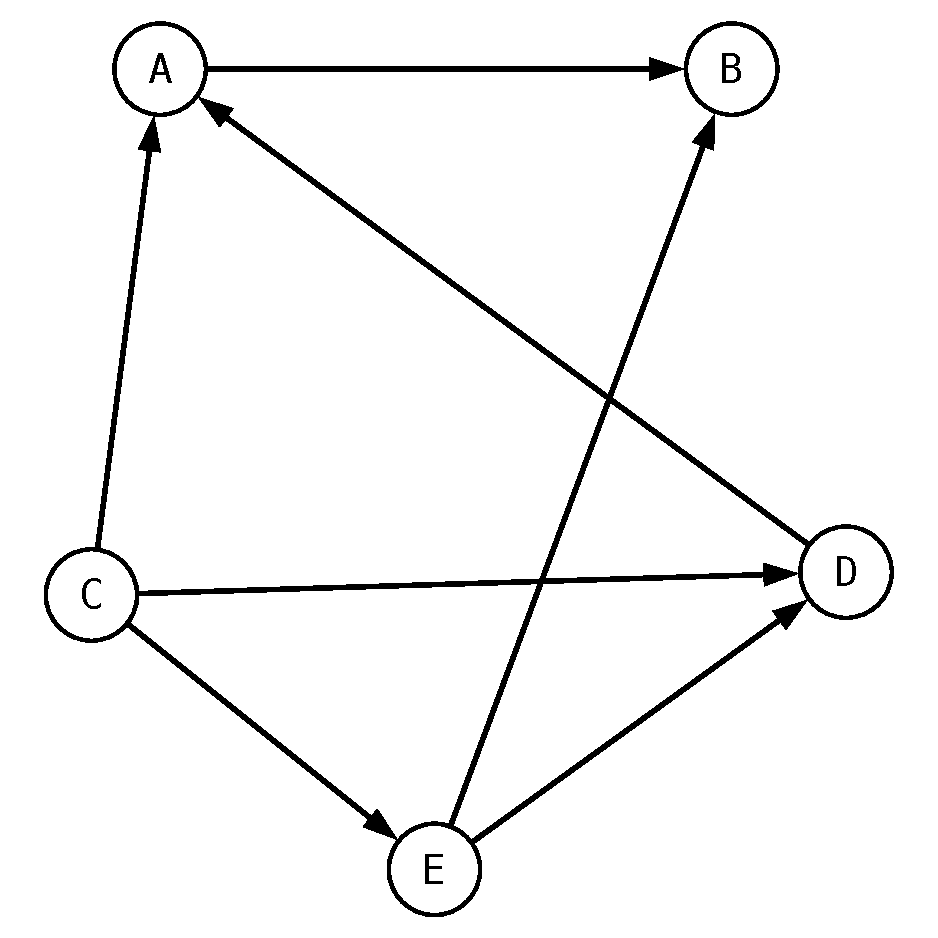
\includegraphics[width=0.5\textwidth]{figures/topsort-initial.pdf}
\end{center}

\noindent Активная ветка DFS --- синяя, текущая вершина --- оранжевая,
тупиковые (уложенные в стек) --- зелёные, рёбра дерева обхода --- зелёные.
Стек показан справа (верх стека --- сверху).

\begin{center}\begin{tabular}{ccc}
\shortstack{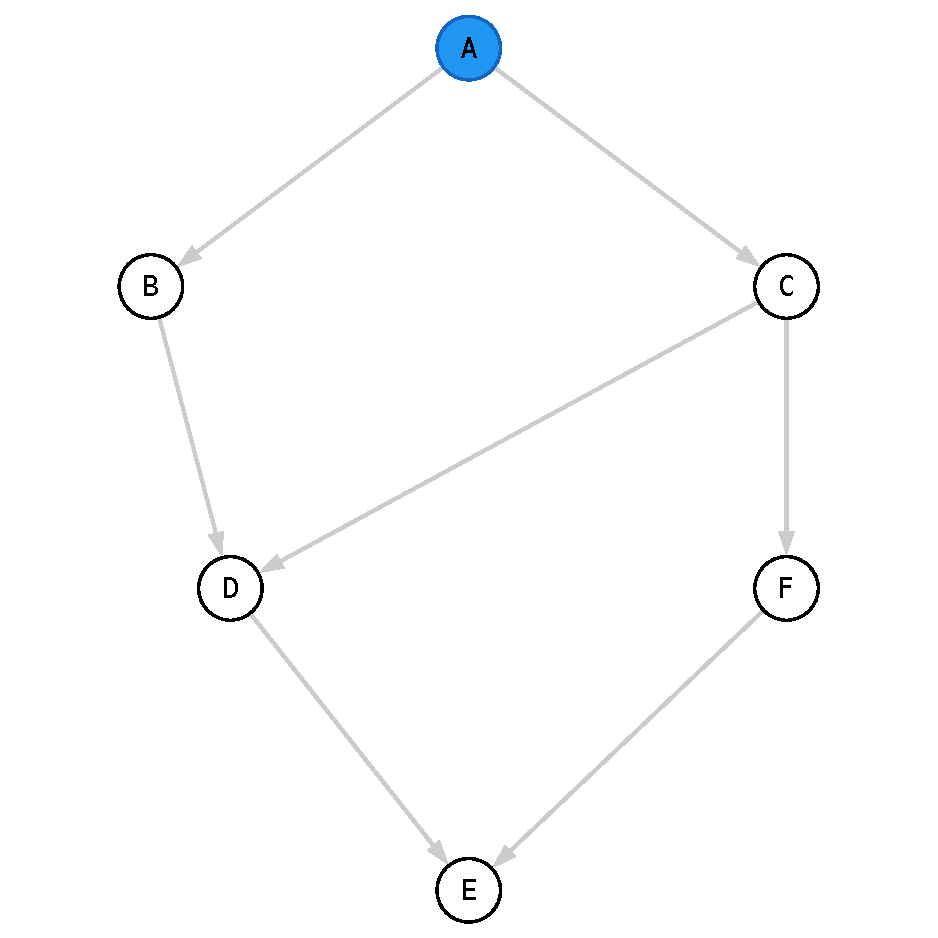
\includegraphics[width=0.30\textwidth]{python/lec02/topsort/topsort-0.pdf}\\[2pt]{\scriptsize Шаг 0. Исходный граф, стек пуст}} &
\shortstack{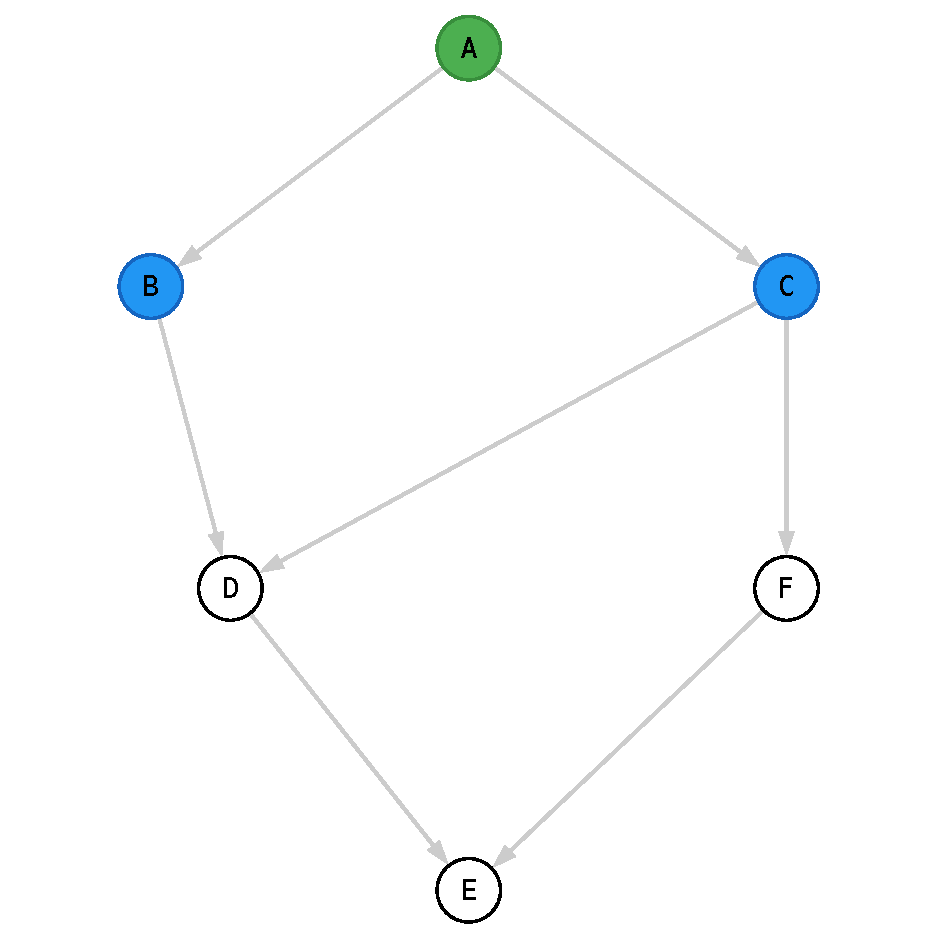
\includegraphics[width=0.30\textwidth]{python/lec02/topsort/topsort-1.pdf}\\[2pt]{\scriptsize Шаг 1. DFS из $A$: идём $A \to B$}} &
\shortstack{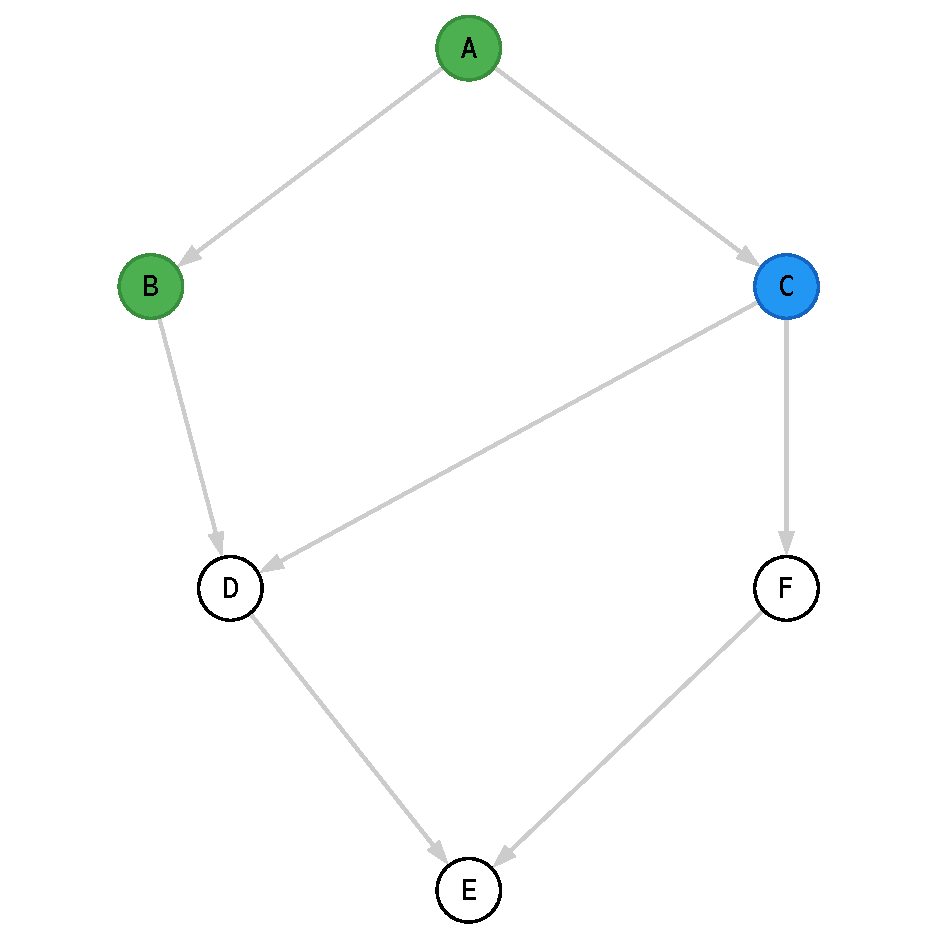
\includegraphics[width=0.30\textwidth]{python/lec02/topsort/topsort-2.pdf}\\[2pt]{\scriptsize Шаг 2. $B$ тупиковая $\to$ в стек}} \\
\end{tabular}\end{center}
\begin{center}\begin{tabular}{ccc}
\shortstack{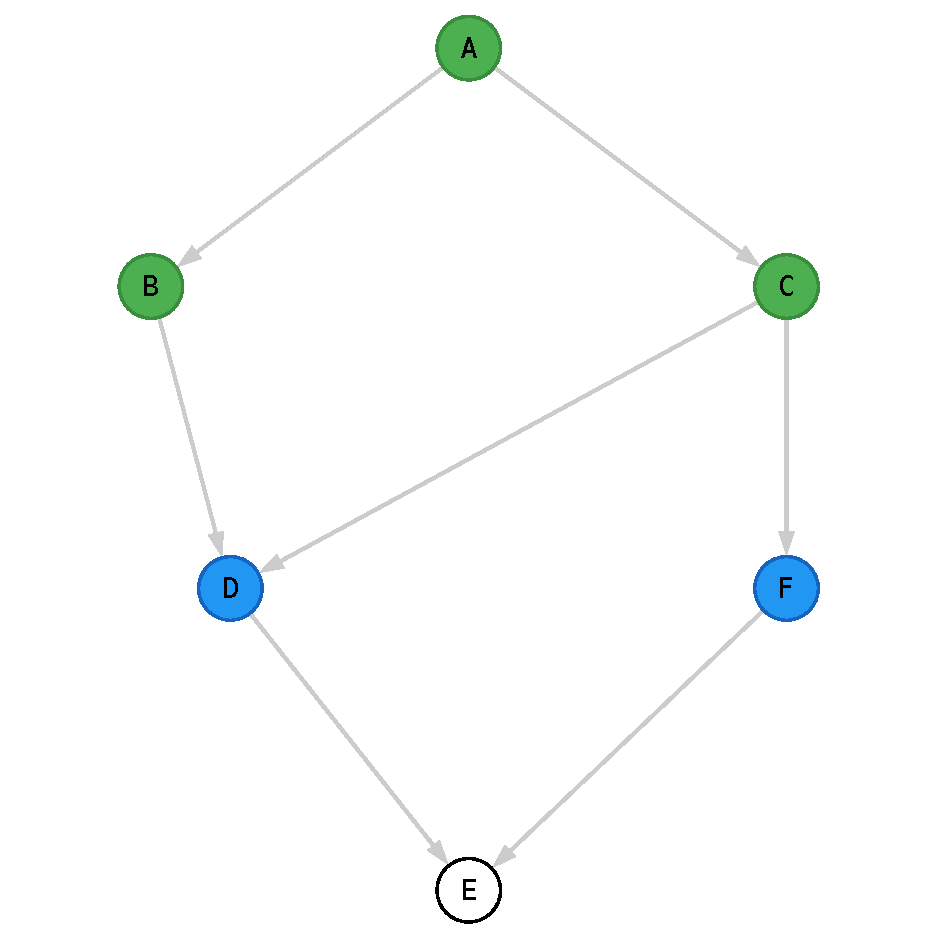
\includegraphics[width=0.30\textwidth]{python/lec02/topsort/topsort-3.pdf}\\[2pt]{\scriptsize Шаг 3. $A$ тупиковая $\to$ в стек}} &
\shortstack{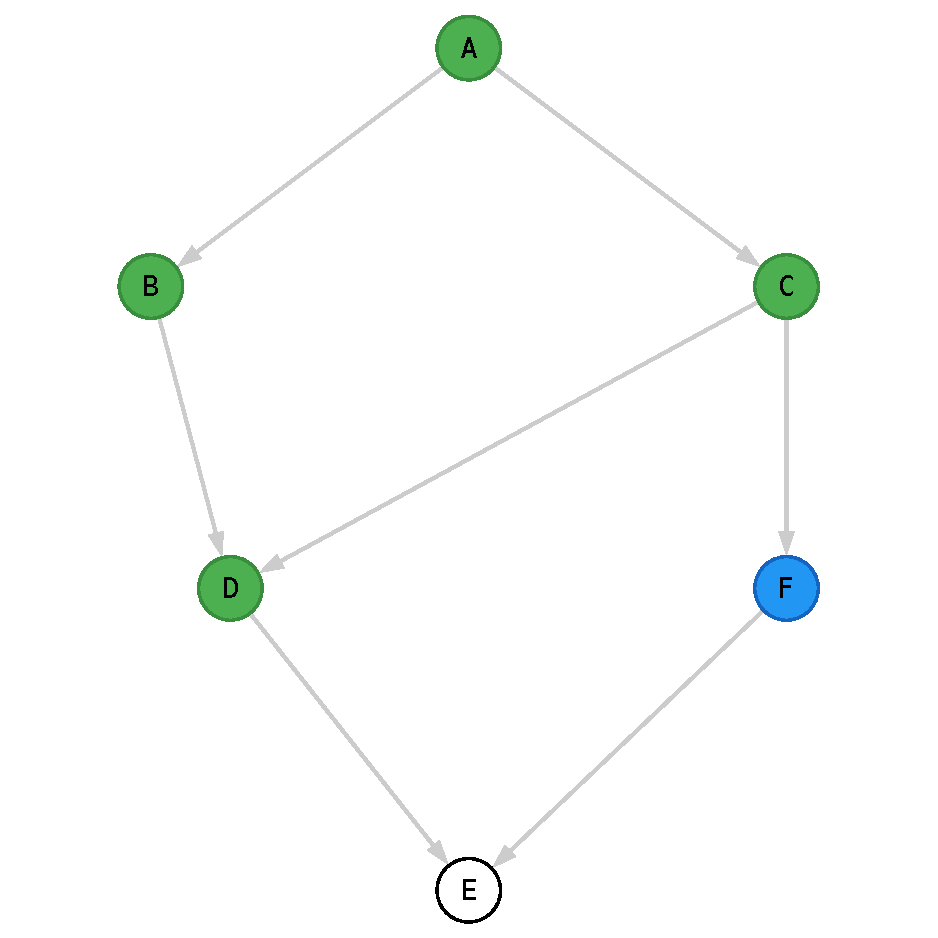
\includegraphics[width=0.30\textwidth]{python/lec02/topsort/topsort-4.pdf}\\[2pt]{\scriptsize Шаг 4. DFS из $C$: $C \to D$; $D \to$ в стек}} &
\shortstack{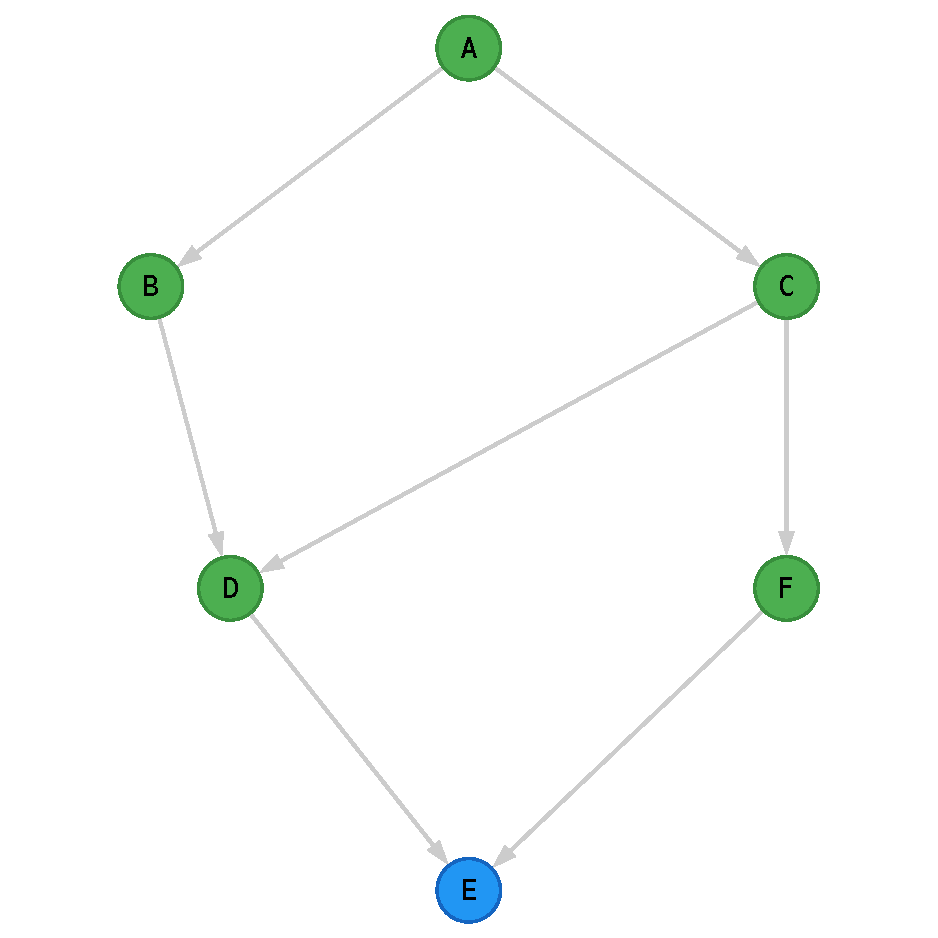
\includegraphics[width=0.30\textwidth]{python/lec02/topsort/topsort-5.pdf}\\[2pt]{\scriptsize Шаг 5. $C \to E$; $E \to$ в стек}} \\
\end{tabular}\end{center}
\begin{center}\begin{tabular}{ccc}
\shortstack{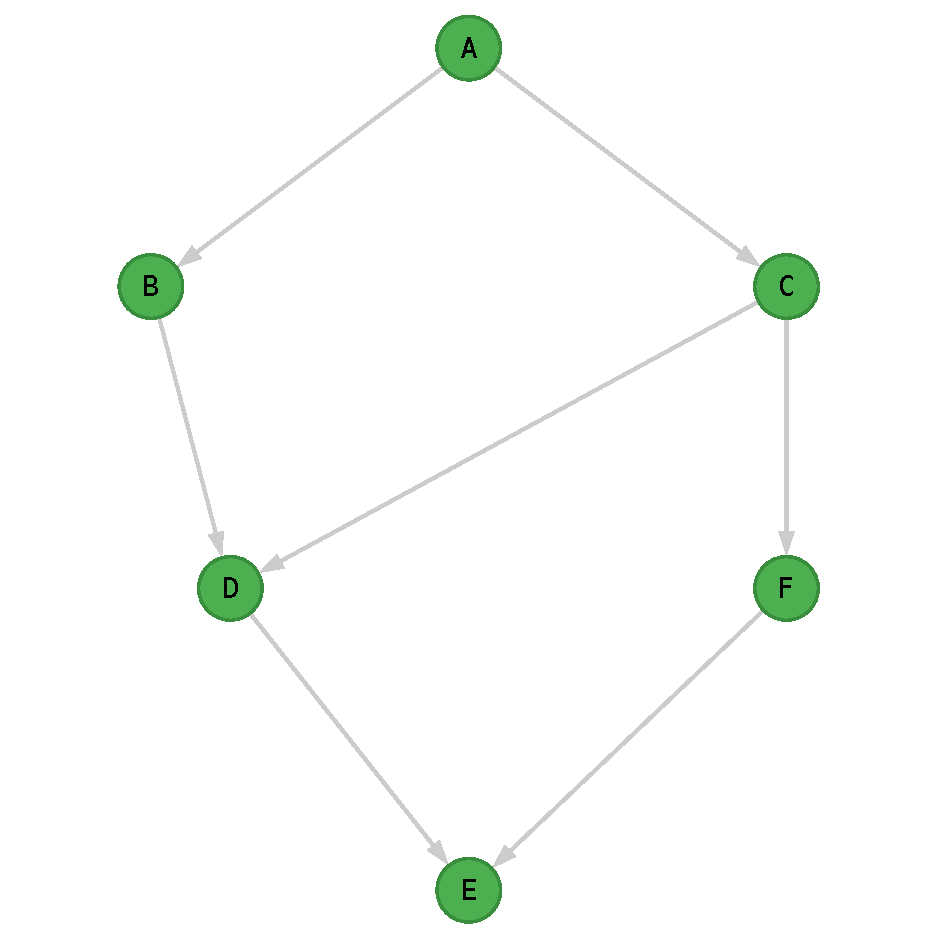
\includegraphics[width=0.30\textwidth]{python/lec02/topsort/topsort-6.pdf}\\[2pt]{\scriptsize Шаг 6. $C$ тупиковая; шаг I завершён}} &
\shortstack{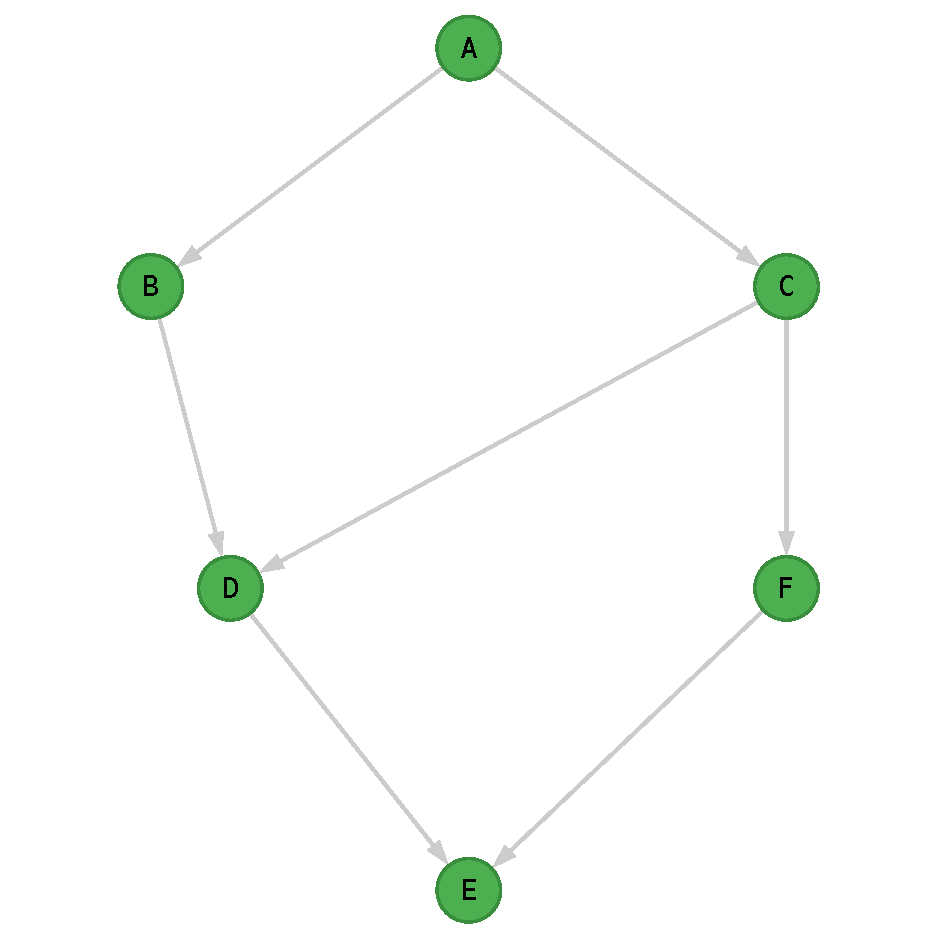
\includegraphics[width=0.30\textwidth]{python/lec02/topsort/topsort-7.pdf}\\[2pt]{\scriptsize Шаг 7. Нумерация по стеку + петли}} &
\shortstack{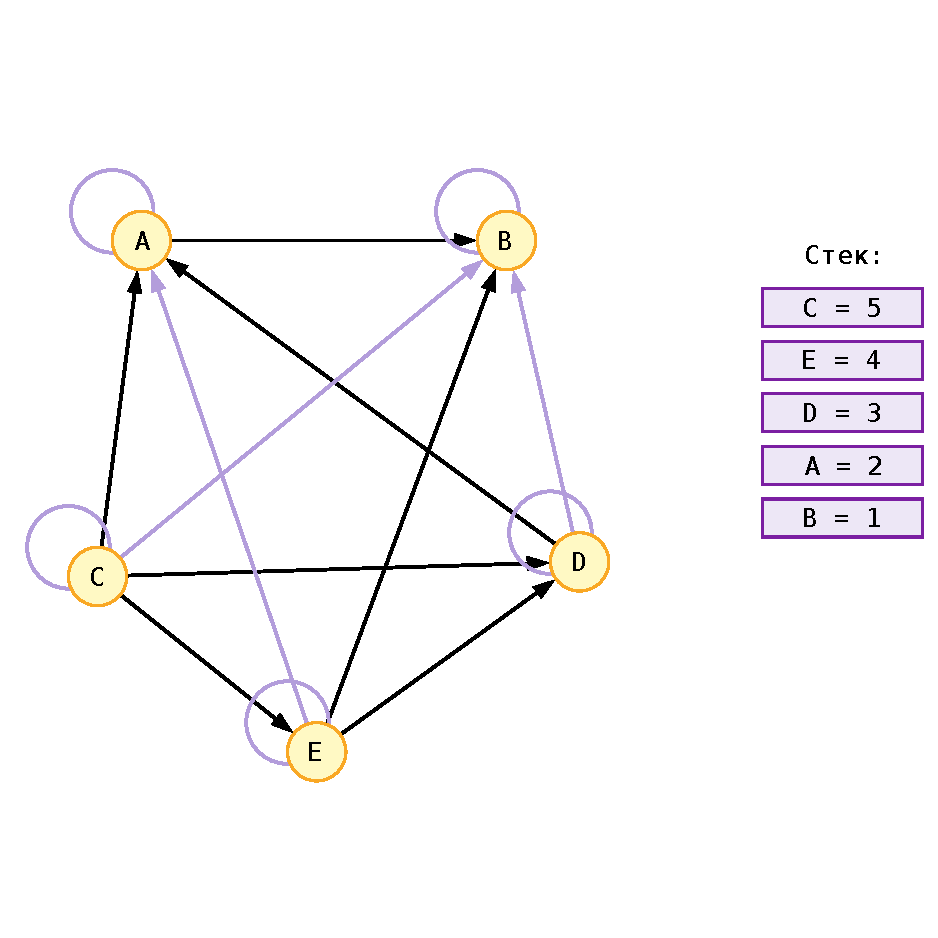
\includegraphics[width=0.30\textwidth]{python/lec02/topsort/topsort-8.pdf}\\[2pt]{\scriptsize Шаг 8. Недостающие рёбра}} \\
\end{tabular}\end{center}

\noindent\textit{Комментарии к шагам.}
На шаге~1 запускаем DFS из $A$: единственное исходящее ребро ведёт в $B$.
У $B$ исходящих рёбер нет --- она тупиковая, кладём её в стек (шаг~2);
возвращаемся в $A$ --- все её рёбра обработаны, $A$ тоже уходит в стек
(шаг~3). Запускаем DFS из следующей непосещённой вершины $C$: ребро
$C \to D$ приводит в $D$, откуда идёт только ребро $D \to A$ в уже
посещённую вершину, поэтому $D$ тупиковая (шаг~4). Далее $C \to E$:
оба ребра из $E$ ($E \to D$, $E \to B$) ведут в посещённые вершины ---
$E$ в стек (шаг~5). Наконец тупиковой становится и $C$ (шаг~6).

На шаге~7 нумеруем вершины по стеку снизу вверх:
$B = 1,\; A = 2,\; D = 3,\; E = 4,\; C = 5$ --- и дорисовываем
рефлексивные петли (светло-фиолетовые). На шаге~8 добавляем недостающие
рёбра из вершин с бóльшими номерами в вершины с меньшими (тоже
светло-фиолетовые: $D \to B$, $E \to A$, $C \to B$ и т.\,д.).

\medskip
Стек (низ $\to$ верх): $B, A, D, E, C$.

Нумерация вершин: $B = 1,\; A = 2,\; D = 3,\; E = 4,\; C = 5$.

Линейный порядок: $B \leq A \leq D \leq E \leq C$.

% Результат: topsort-result-0.graph
\grfig[0.45]{figures/topsort-result-0.pdf}{Результат Topsort --- линейный порядок $B \leq A \leq D \leq E \leq C$}
\end{algo}


\chapter{Лекция 3. Строгий порядок. Замыкания. Основы теории графов}

% === Строгий порядок ===

\begin{defn}{Строгий порядок}{strict-order}
$M \neq \varnothing$,\; $f\colon M^2 \to \mathbb{B}$.

$f$ --- \textbf{строгий порядок} $\;\Leftrightarrow\;$
$f$ асимметрично и транзитивно.
\end{defn}

\textbf{Пример:} $\mathbb{R},\; <$.

\begin{task}{}{task-asym}
Доказать, что асимметричность $\Rightarrow$ арефлексивность.
\tcblower
\textbf{Решение.} Асимметричность: $\forall\, a, b\colon
f(a,b) = 1 \Rightarrow f(b,a) = 0$. Возьмём $b = a$: если бы нашлось $a$
с $f(a,a) = 1$, то по асимметричности (при $b = a$) получили бы
$f(a,a) = 0$ --- противоречие. Значит $\forall\, a\colon f(a,a) = 0$,
т.\,е. отношение арефлексивно. $\blacksquare$
\end{task}

% === Замыкания ===
\bigskip
\begin{defn}{Замыкание бинарного отношения}{closure}
$M \neq \varnothing$,\; $f\colon M^2 \to \mathbb{B}$,\;
$\tilde{f}\colon M^2 \to \mathbb{B}$.

\textbf{Замыкание} $f$ относительно свойства $(*)$ --- это $\tilde{f}$, т.\,ч.:
\begin{enumerate}
  \item $\tilde{f}$ согласовано с $f$
        (т.\,е. $\forall\, a,b\colon f(a,b)=1 \Rightarrow \tilde{f}(a,b)=1$);
  \item $\tilde{f}$ обладает свойством $(*)$;
  \item $\tilde{f}$ имеет минимальный носитель среди всех б.\,о.,
        удовлетворяющих 1) и 2) (минимальное количество рёбер).
\end{enumerate}
\end{defn}

\begin{defn}{Носитель функции}{support}
$f\colon A \to B$. \textbf{Носитель} $f$:
\[
  \operatorname{supp}(f) := \bigl\{\, a \in A \;\big|\; f(a) \neq 0 \,\bigr\}.
\]
\end{defn}

\textit{Замечание:} замыкать можно только <<вверх>> (добавлять рёбра).
Например, замыкание по арефлексивности невозможно --- нельзя стирать рёбра.

\medskip
\textbf{Примеры замыканий.}

\begin{enumerate}
  \item \textbf{Рефлексивное замыкание:}
        граф $a \to b \to c$ --- добавляем петли у каждой вершины.

  \item \textbf{Симметричное замыкание:}
        $a \to b$, $b \to c$ --- добавляем обратные рёбра
        ($b \to a$, $c \to b$).
\end{enumerate}

\textbf{NB:} после рефлексивного и симметричного замыканий может нарушиться
транзитивность: $a \to b$ и $b \to c$ есть, но $a \to c$ нет
(транзитивная дуга отсутствует).

% === Алгоритм Флойда--Уоршелла ===
\bigskip
\begin{algo}{Алгоритм Флойда--Уоршелла (построение транзитивного замыкания)}{floyd-warshall-closure}
\textbf{Вход:} матрица смежности $A_f$ б.\,о. $f$ (размер $n \times n$).

\textbf{Выход:} матрица транзитивного замыкания $\tilde{A}$.

\textbf{Шаг 1:} $\forall\, v \in V$: рассматриваем $v$ как <<промежуточную>> вершину.

\textbf{Шаг 2:} Для каждой пары $(i, j)$: если $a_{iv} = 1$ и $a_{vj} = 1$,
то полагаем $a_{ij} := 1$.

Повторяем для всех вершин $v$.

После дорисовывания графа получаем транзитивное замыкание.
\end{algo}

\exhead{Пример.} Граф $a \to b \to c \to d$. Проследим работу алгоритма
сразу в двух представлениях: на графе и на матрице смежности. Новые
(дорисованные на текущем шаге) рёбра --- зелёные, добавленные ранее ---
светло-фиолетовые; промежуточная вершина $v$ --- оранжевая. В матрицах
новые единицы выделены жирным.

\medskip
\noindent Исходный граф и его матрица ($v = a$ ничего не даёт: в $a$ нет
входящих рёбер):

\begin{center}
\begin{tabular}{cc}
\raisebox{-0.5\height}{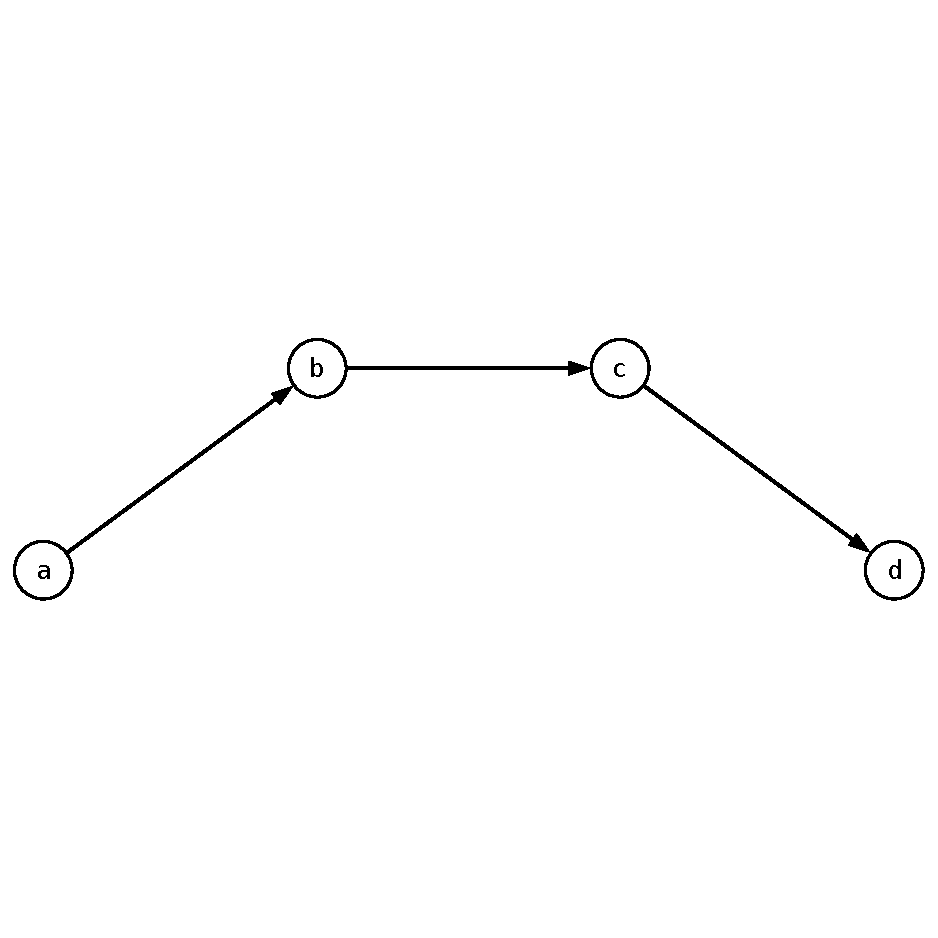
\includegraphics[width=0.42\textwidth]{figures/fw-step-0.pdf}} &
\renewcommand{\arraystretch}{1.25}
\begin{tabular}{|c||c|c|c|c|}
\hline
$f$ & \textbf{a} & \textbf{b} & \textbf{c} & \textbf{d} \\ \hline\hline
\textbf{a} & 0 & 1 & 0 & 0 \\ \hline
\textbf{b} & 0 & 0 & 1 & 0 \\ \hline
\textbf{c} & 0 & 0 & 0 & 1 \\ \hline
\textbf{d} & 0 & 0 & 0 & 0 \\ \hline
\end{tabular}
\end{tabular}
\end{center}

\noindent Промежуточная вершина $v = b$: есть $a \to b$ и $b \to c$,
поэтому дорисовываем $a \to c$ (т.\,е. $a_{ac} := 1$):

\begin{center}
\begin{tabular}{cc}
\raisebox{-0.5\height}{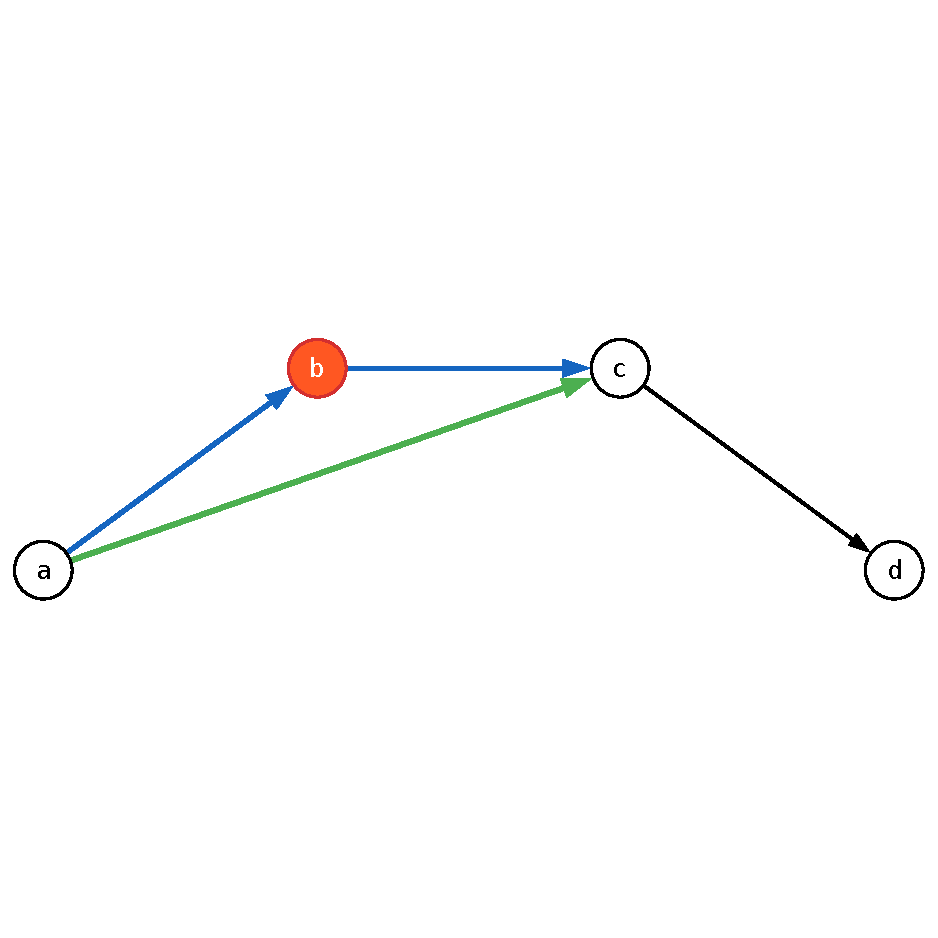
\includegraphics[width=0.42\textwidth]{figures/fw-step-1.pdf}} &
\renewcommand{\arraystretch}{1.25}
\begin{tabular}{|c||c|c|c|c|}
\hline
$f$ & \textbf{a} & \textbf{b} & \textbf{c} & \textbf{d} \\ \hline\hline
\textbf{a} & 0 & 1 & $\mathbf{1}$ & 0 \\ \hline
\textbf{b} & 0 & 0 & 1 & 0 \\ \hline
\textbf{c} & 0 & 0 & 0 & 1 \\ \hline
\textbf{d} & 0 & 0 & 0 & 0 \\ \hline
\end{tabular}
\end{tabular}
\end{center}

\noindent Промежуточная вершина $v = c$: в $c$ входят $a \to c$ и $b \to c$,
из $c$ выходит $c \to d$, поэтому дорисовываем $a \to d$ и $b \to d$:

\begin{center}
\begin{tabular}{cc}
\raisebox{-0.5\height}{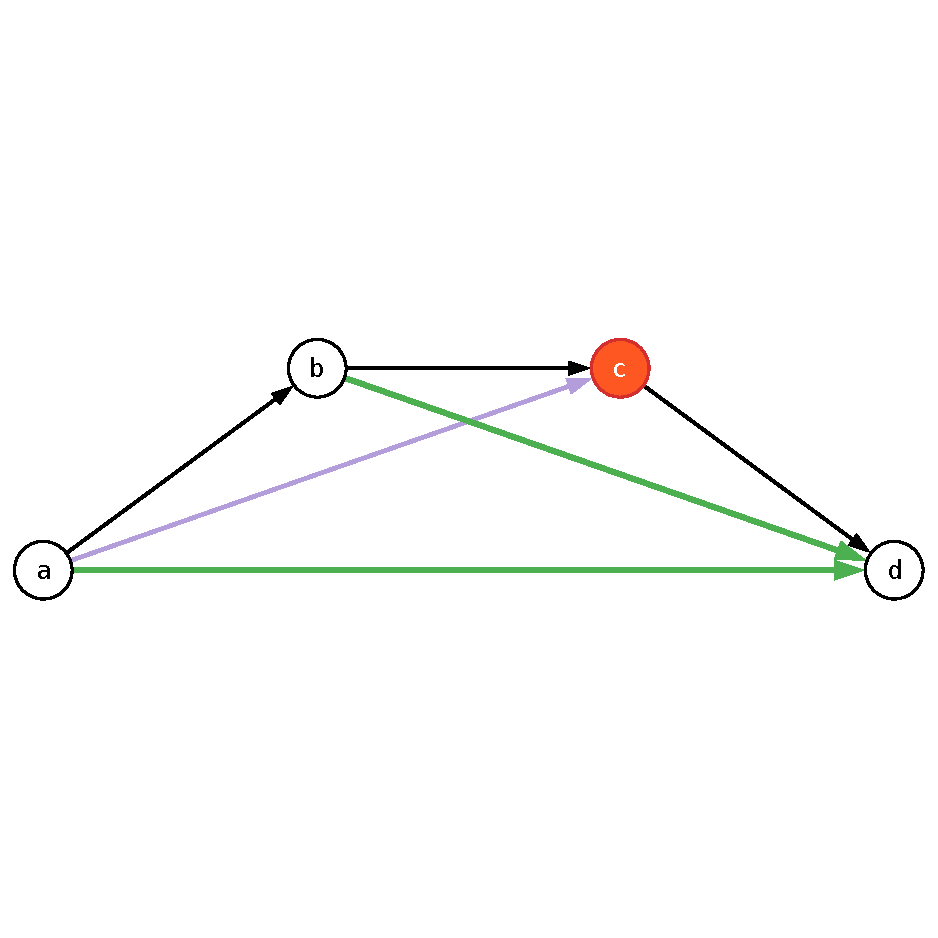
\includegraphics[width=0.42\textwidth]{figures/fw-step-2.pdf}} &
\renewcommand{\arraystretch}{1.25}
\begin{tabular}{|c||c|c|c|c|}
\hline
$f$ & \textbf{a} & \textbf{b} & \textbf{c} & \textbf{d} \\ \hline\hline
\textbf{a} & 0 & 1 & 1 & $\mathbf{1}$ \\ \hline
\textbf{b} & 0 & 0 & 1 & $\mathbf{1}$ \\ \hline
\textbf{c} & 0 & 0 & 0 & 1 \\ \hline
\textbf{d} & 0 & 0 & 0 & 0 \\ \hline
\end{tabular}
\end{tabular}
\end{center}

\noindent Промежуточная вершина $v = d$ ничего не добавляет (из $d$ нет
исходящих рёбер). Итог --- транзитивное замыкание
$\tilde f = \{a{\to}b,\; b{\to}c,\; c{\to}d,\; a{\to}c,\; a{\to}d,\; b{\to}d\}$:

\begin{center}
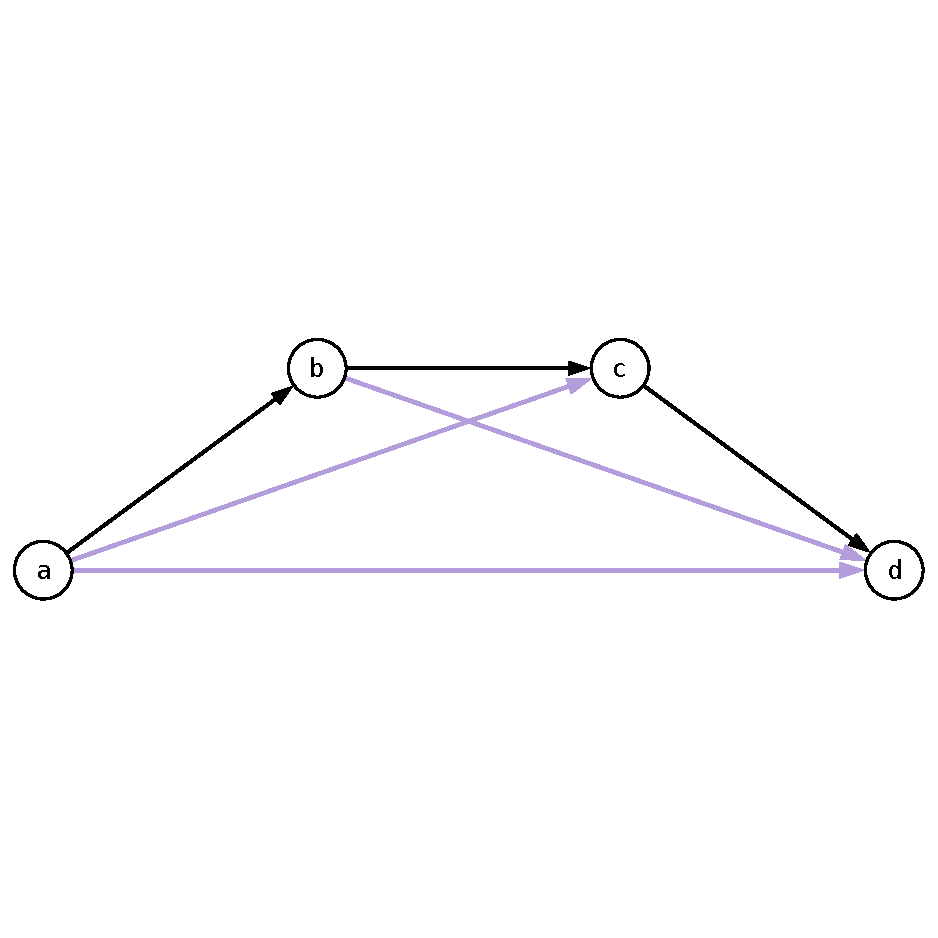
\includegraphics[width=0.42\textwidth]{figures/fw-step-3.pdf}
\end{center}

% === Основы теории графов ===
\bigskip
\subsection*{Основные понятия теории графов}

$G(V, E)$ --- \textbf{граф}, где $V$ --- множество вершин, $E$ --- множество рёбер.

Граф бывает:
\begin{itemize}
  \item \textbf{неориентированный} (ненаправленный) --- рёбра без направления;
  \item \textbf{ориентированный} (направленный) --- хотя бы одно ориентированное ребро.
\end{itemize}

Рёбра: ориентированные / неориентированные. Также: петля, цикл, путь.

Связный граф. Компоненты связности. Дерево. Подграф.

\bigskip
\textbf{Вершины:}
\begin{itemize}
  \item \textbf{Изолированная} --- степени 0.
  \item \textbf{Висячая} --- степени 1.
\end{itemize}

\textbf{Рёбра:}
\begin{itemize}
  \item Петля --- ребро из вершины в себя.
  \item Ориентированное ребро $a \to b$: $a$ --- родитель, $b$ --- потомок
        (только для ориент. графов).
\end{itemize}

Неориентированный ненаправленный граф --- без дублирующих рёбер.

Ориентированный направленный граф --- хотя бы одно ориент. ребро.

\textbf{Смежность.} Вершины $a, b$ \textbf{смежные}, если между ними есть ребро.

$e$ --- ребро, \textbf{инцидентное} вершине $a$ и вершине $b$.

\bigskip
\begin{defn}{Степень вершины}{vertex-degree}
\textbf{Степень вершины} (для неор. графа) --- количество инцидентных ей рёбер:
\[
  \deg(v).
\]
Пусть $G(V, E)$, $|V| = n$. Тогда $0 \leq \deg(v) \leq n - 1$.
\end{defn}

\textbf{Регулярный граф} --- все вершины одинаковой степени.

\medskip
\textbf{В ориентированном графе:}
\begin{itemize}
  \item $\delta^+(v) = \#\bigl\{u \in V \;\big|\; \exists\, e\colon u \to v\bigr\}$
        --- количество входящих рёбер;
  \item $\delta^-(v) = \#\bigl\{u \in V \;\big|\; \exists\, e\colon v \to u\bigr\}$
        --- количество выходящих рёбер.
\end{itemize}

\bigskip
\textbf{Путь} из вершины $A$ в вершину $B$ --- непрерывная последовательность рёбер,
первое из которых начинается в $A$, последнее заканчивается в $B$.

Последовательность \textbf{непрерывная} --- конец предыдущего ребра совпадает
с началом следующего.

\textbf{Простой путь} --- без повторяющихся рёбер.

\textbf{Цепь} --- простой путь, в котором вершины тоже не повторяются.

\textbf{Открытый путь} --- начало и конец различны.
\textbf{Замкнутый путь} --- начало и конец совпадают.

\textbf{Цикл} --- замкнутый простой путь (без повторяющихся рёбер).

$C_n$ --- замкнутая цепь на $n$ вершинах.

\bigskip
\begin{defn}{Полный граф}{complete-graph}
\textbf{Полный граф} $K_n$ --- граф, в котором любые две вершины смежные.
\end{defn}

\begin{defn}{Дерево}{tree-rel}
Граф называется \textbf{деревом}, если он связный и ациклический.
\end{defn}

$T_n$ --- дерево на $n$ вершинах. При $n \geq 4$ дерево определено неоднозначно
(существуют разные деревья с одинаковым числом вершин).

\begin{defn}{Лес}{forest}
Граф называется \textbf{лесом}, если он ациклический (связность
\emph{не} требуется). Эквивалентно: лес --- граф, каждая компонента
связности которого является деревом; дерево --- это связный лес.
\end{defn}

\grfig[0.5]{figures/p7-forest-1.pdf}{Лес из трёх компонент: два дерева и изолированная вершина}

\textbf{Примеры.} Граф на рисунке --- лес из трёх деревьев:
$\{A, B, C, D\}$, $\{E, F\}$ и одиночной вершины $\{H\}$ (изолированная
вершина --- тоже дерево). Если у леса $n$ вершин и $k$ компонент, то
рёбер ровно $n - k$ (по $n_i - 1$ в каждой компоненте). Другой пример:
любой ациклический подграф любого графа --- лес; в частности, остовное
дерево без одного ребра --- лес из двух деревьев.

\begin{defn}{Связный граф}{connected-graph}
\textbf{Связный граф} --- между любыми двумя вершинами $\exists$ путь.
\end{defn}

\begin{defn}{Компонента связности}{connected-component}
\textbf{Компонента связности} --- максимальный по включению связный подграф.
\end{defn}

% Пример: граф с 3 компонентами связности (p8-componenta-svyaznosti.graph)
\grfig[0.45]{figures/p8-componenta-svyaznosti.pdf}{3 компоненты связности (9 вершин)}
% {A, B, C, D, E} --- одна компонента, {F, H} --- вторая, {I, J} --- третья.
% Рёбра: B--C, C--D, C--E, F--H, H--I, H--J.

\bigskip
\begin{statement}{Лемма о рукопожатиях}{handshake-lemma}
$G(V, E)$ --- неориентированный граф. Тогда:
\[
  \sum_{v \in V} \deg(v) = 2|E|.
\]
\end{statement}

\begin{proof}
Посчитаем пары $(v, e)$, где ребро $e$ инцидентно вершине $v$, двумя
способами. С одной стороны, каждая вершина $v$ участвует ровно в $\deg(v)$
таких парах, всего $\sum_{v \in V} \deg(v)$. С другой стороны, каждое ребро
$e = \{u, w\}$ инцидентно ровно двум вершинам, т.\,е. участвует ровно в двух
парах; всего $2|E|$. Значит, $\sum_{v} \deg(v) = 2|E|$.
\end{proof}

\begin{statement}{Лемма о чётности}{parity-lemma}
$G(V, E)$ --- неориентированный граф. Тогда количество вершин нечётной степени чётно:
\[
  \#\bigl\{\, v \in V \;\big|\; \deg(v) \;\not\vdots\; 2 \,\bigr\} \;\vdots\; 2.
\]
\end{statement}

\begin{proof}
Разобьём вершины на два множества: $V_{\text{ч}}$ --- вершины чётной степени
и $V_{\text{н}}$ --- вершины нечётной степени. По лемме о рукопожатиях
\[
  \underbrace{\sum_{v \in V_{\text{ч}}} \deg(v)}_{\text{чётно}}
  + \sum_{v \in V_{\text{н}}} \deg(v) = 2|E| \quad\text{--- чётно},
\]
поэтому $\sum_{v \in V_{\text{н}}} \deg(v)$ тоже чётно. Но это сумма
\emph{нечётных} слагаемых, а сумма $k$ нечётных чисел чётна тогда и только
тогда, когда $k$ чётно. Значит, $|V_{\text{н}}|$ чётно.
\end{proof}

\begin{statement}{Лемма о числе рёбер полного графа}{complete-graph-edges}
\[
  |E_{K_n}| = \frac{n(n-1)}{2}.
\]
\end{statement}

\begin{proof}
В $K_n$ любые две различные вершины соединены ровно одним ребром, поэтому
рёбра взаимно однозначно соответствуют неупорядоченным парам вершин:
$|E_{K_n}| = \binom{n}{2} = \frac{n(n-1)}{2}$. Иначе: каждая из $n$ вершин
имеет степень $n-1$, и по лемме о рукопожатиях
$|E| = \frac{1}{2}\sum_v \deg(v) = \frac{n(n-1)}{2}$.
\end{proof}

\begin{task}{}{task-tree-edges}
Доказать: если $G(V, E)$ --- связный граф, $|V| = n$, $|E| = n - 1$,
то $G$ --- дерево.
\tcblower
\textbf{Решение.} Дерево --- связный ациклический граф, и связность дана,
поэтому достаточно показать, что в $G$ нет циклов. Предположим противное:
в $G$ есть цикл. Удалим любое ребро $e$ этого цикла --- граф
$G' = G - e$ останется связным (любой путь, проходивший через $e$, можно
провести в обход по оставшейся части цикла), и в нём $n - 2$ ребра.
Будем повторять: пока в графе остаются циклы, удаляем по одному
рёбру цикла, сохраняя связность. Процесс конечен и закончится связным
ациклическим графом (деревом) $T$ на тех же $n$ вершинах, в котором
\emph{меньше} чем $n-1$ рёбер. Но любой связный граф на $n$ вершинах
содержит не менее $n - 1$ ребра (см. лемму о связности ниже: каждая новая
вершина при построении связного графа требует хотя бы одного нового ребра)
--- противоречие. Значит, циклов в $G$ не было, и $G$ --- дерево.
$\blacksquare$
\end{task}

\begin{statement}{Лемма о связности}{connectivity-lemma}
$G(V, E)$ --- неориентированный связный граф, $|V| = n$. Тогда:
\[
  (n - 1) \leq |E| \leq \frac{n(n-1)}{2}.
\]
\end{statement}

\begin{proof}
\textbf{Верхняя оценка.} Рёбер не может быть больше, чем всех
неупорядоченных пар вершин, т.\,е. $|E| \le \binom{n}{2} =
\frac{n(n-1)}{2}$ (максимум достигается на полном графе $K_n$).

\textbf{Нижняя оценка} (индукция по $n$). База: при $n = 1$ имеем
$|E| \ge 0 = n - 1$. Переход: пусть утверждение верно для всех связных
графов с числом вершин меньше $n$. Возьмём связный граф $G$ на $n \ge 2$
вершинах и удалим из него вершину $v$ минимальной степени вместе с
инцидентными ей рёбрами (их $\deg(v) \ge 1$, так как изолированных вершин
в связном графе при $n \ge 2$ нет). Граф может распасться на
$k \le \deg(v)$ компонент связности с числом вершин $n_1, \dots, n_k$,
$n_1 + \dots + n_k = n - 1$. По предположению индукции в $i$-й компоненте
не менее $n_i - 1$ рёбер, итого
\[
  |E| \;\ge\; \deg(v) + \sum_{i=1}^{k}(n_i - 1)
  \;=\; \deg(v) + (n - 1) - k \;\ge\; n - 1,
\]
поскольку $k \le \deg(v)$. Оценка точна: у дерева ровно $n-1$ ребро.
\end{proof}


\chapter{Лекция 4. Метрические характеристики графа. Способы представления. Связность}

% === Метрические характеристики ===

$G(V, E)$ --- неориентированный, связный граф.

\begin{defn}{Расстояние между вершинами}{distance}
$\forall\, u, v \in V$:
\[
  \operatorname{dist}(u, v) := \min l,
\]
где $l$ --- длина пути $u \to \ldots \to v$.

Свойства:
\begin{itemize}
  \item $\operatorname{dist}(u, u) = 0$;
  \item $\operatorname{dist}(u, v) = \operatorname{dist}(v, u)$.
\end{itemize}
\end{defn}

\begin{defn}{Эксцентриситет вершины}{eccentricity}
$v \in V$:
\[
  \varepsilon(v) := \max_{u \in V} \bigl\{\operatorname{dist}(u, v)\bigr\}.
\]
\end{defn}

\begin{defn}{Радиус графа}{radius}
\[
  R(G) := \min_{v \in V} \bigl\{\varepsilon(v)\bigr\}.
\]
\end{defn}

\begin{defn}{Диаметр графа}{diameter}
\[
  D(G) := \max_{v \in V} \bigl\{\varepsilon(v)\bigr\}.
\]
\end{defn}

\begin{defn}{Центр графа}{center}
\[
  \operatorname{Cent}(G) := \bigl\{\, u \in V \;\big|\; \varepsilon(u) = R(G) \,\bigr\}.
\]
\end{defn}

\bigskip
% --- Пример 0: p9-example-0.graph ---
\exhead{Пример 1.}
% Граф: p9-example-0.graph
\grfig{figures/p9-example-0.pdf}{Метрики: 7 вершин, $R=3$, $D=5$}
% Вершины: A, B, C, D, E, F, H
% Рёбра: A--B, B--C, C--E, D--B, D--E, C--D, E--F, F--H

Как считаются эксцентриситеты: для каждой вершины выписываем, какие
вершины достижимы ровно за 1, 2, 3, \dots{} шагов (поиск в ширину);
номер последнего непустого столбца и есть $\varepsilon(v)$ ---
расстояние до самой дальней вершины.

\medskip
\begin{center}
\begin{tabular}{c|l|l|l|l|l|c}
  верш. & за 1 шаг & за 2 шага & за 3 шага & за 4 шага & за 5 шагов & $\varepsilon$ \\ \hline
  $A$ & $B$       & $C, D$    & $E$       & $F$ & $H$ & 5 \\
  $B$ & $A, C, D$ & $E$       & $F$       & $H$ &     & 4 \\
  $C$ & $B, D, E$ & $A, F$    & $H$       &     &     & 3 \\
  $D$ & $B, C, E$ & $A, F$    & $H$       &     &     & 3 \\
  $E$ & $C, D, F$ & $B, H$    & $A$       &     &     & 3 \\
  $F$ & $E, H$    & $C, D$    & $B$       & $A$ &     & 4 \\
  $H$ & $F$       & $E$       & $C, D$    & $B$ & $A$ & 5 \\
\end{tabular}
\end{center}

\medskip
Эксцентриситеты:
$\varepsilon(A) = 5$,\;
$\varepsilon(B) = 4$,\;
$\varepsilon(C) = 3$,\;
$\varepsilon(D) = 3$,\;
$\varepsilon(E) = 3$,\;
$\varepsilon(F) = 4$,\;
$\varepsilon(H) = 5$.

Минимум эксцентриситетов даёт радиус, максимум --- диаметр:
$R(G) = 3$,\quad $D(G) = 5$,\quad $\operatorname{Cent}(G) = \{C, D, E\}$.

\medskip
% --- Пример 1: p9-example-1.graph ---
\exhead{Пример 2.}
% Граф: p9-example-1.graph
\grfig{figures/p9-example-1.pdf}{Метрики: цикл $C_5$, $R=D=2$}
% Вершины: A, B, C, D, E (цикл C_5)
% Рёбра: A--B, B--E, E--D, D--C, C--A

Цикл $C_5$: $A$--$B$--$E$--$D$--$C$--$A$.

Здесь всё симметрично, достаточно посчитать для одной вершины: например,
от $A$ за 1 шаг достижимы соседи $B$ и $C$, за 2 шага --- остальные две
вершины $E$ и $D$, поэтому $\varepsilon(A) = 2$; по симметрии цикла так же
для всех остальных вершин.

Эксцентриситеты: $\varepsilon(A) = \varepsilon(B) = \varepsilon(C) = \varepsilon(D) = \varepsilon(E) = 2$.

$R(G) = 2$,\quad $D(G) = 2$,\quad $\operatorname{Cent}(G) = \{A, B, C, D, E\} = V$.

\medskip
\textbf{Полный граф:}
$D(K_n) = 1$,\; $R(K_n) = 1$,\; $\operatorname{Cent}(K_n) = V_{K_n}$.

% === Вычисление метрических характеристик (пример с деревом) ===
\bigskip
\textbf{Вычисление метрических характеристик графа.}

\textbf{Алгоритм} (I): Для дерева (без циклов):
$D(G) = \max$ длина цепи,\;
$R(G) = \left\lceil \dfrac{D(G)}{2} \right\rceil$.

% --- Пример: p10-example-1.graph (дерево, 14 вершин) ---
\exhead{Пример (дерево).}
% Граф: p10-example-1.graph
\grfig{figures/p10-example-1.pdf}{Метрики: дерево 14 вершин}
% Вершины: A, B, C, D, E, F, H, I, J, K, L, R, P, Q
% Рёбра: A--B, B--C, C--D, D--E, E--F, F--H, I--J, J--K, K--L, E--I, C--R, C--P, P--Q

Для дерева не нужно считать все расстояния: ищем самую длинную цепь
(\emph{диаметральную цепь}). Здесь это, например,
\[
  A - B - C - D - E - I - J - K - L
\]
длины $8$ (другая такая же: $Q$--$P$--$C$--$D$--$E$--$I$--$J$--$K$--$L$).
Следовательно $D(G) = 8$ и $R(G) = \lceil 8/2 \rceil = 4$, а центр ---
середина диаметральной цепи, вершина $E$: она удалена ровно на $4$ от
обоих концов цепи ($A$ и $L$), и дальше чем на $4$ от неё ничего нет
(проверка: за 1 шаг от $E$ достижимы $D, F, I$; за 2 --- $C, H, J$;
за 3 --- $B, R, P, K$; за 4 --- $A, Q, L$, т.\,е. $\varepsilon(E) = 4$).

\medskip
Эксцентриситеты (для проверки):
$\varepsilon(A) = 8$,\;
$\varepsilon(B) = 7$,\;
$\varepsilon(C) = 6$,\;
$\varepsilon(D) = 5$,\;
$\varepsilon(E) = 4$,\;
$\varepsilon(F) = 5$,\;
$\varepsilon(H) = 6$,\;
$\varepsilon(I) = 5$,\;
$\varepsilon(J) = 6$,\;
$\varepsilon(K) = 7$,\;
$\varepsilon(L) = 8$,\;
$\varepsilon(R) = 7$,\;
$\varepsilon(P) = 7$,\;
$\varepsilon(Q) = 8$.

$R(G) = 4$,\quad $D(G) = 8$,\quad $\operatorname{Cent}(G) = \{E\}$.

% === (II) Граф содержит хотя бы один цикл ===
\bigskip
\textbf{(II) Граф содержит хотя бы один цикл.}

% Граф: p10-example-5.graph
\grfig{figures/p10-example-5.pdf}{Метрики: 11 вершин с циклами}
% Вершины: A, B, C, D, E, H, I, J, F, K, L (11 вершин)
% Рёбра: A--B, B--C, C--D, H--I, I--J, F--K, A--H, H--C, H--D, J--L, I--K, K--H, F--H, A--E, E--F

Списки смежности:

\begin{tabular}{c|l}
  верш. & смежные \\ \hline
  $A$ & $B, E, H$ \\
  $B$ & $A, C$ \\
  $C$ & $B, D, H$ \\
  $D$ & $C, H$ \\
  $E$ & $A, F$ \\
  $F$ & $E, H, K$ \\
  $H$ & $A, C, D, F, I, K$ \\
  $I$ & $H, J, K$ \\
  $J$ & $I, L$ \\
  $K$ & $F, H, I$ \\
  $L$ & $J$ \\
\end{tabular}

\medskip
Таблица достижимости:

\begin{tabular}{c|l|l|l|l|l}
  верш. & за 1 шаг & за 2 шага & за 3 шага & за 4 шага & за 5 шагов \\ \hline
  $A$ & $B, E, H$ & $C, D, F, I, K$ & $J$ & $L$ & \\
  $B$ & $A, C$ & $D, E, H$ & $F, I, K$ & $J$ & $L$ \\
  $C$ & $B, D, H$ & $A, F, I, K$ & $E, J$ & $L$ & \\
  $D$ & $C, H$ & $A, B, F, I, K$ & $E, J$ & $L$ & \\
  $E$ & $A, F$ & $B, H, K$ & $C, D, I$ & $J$ & $L$ \\
  $F$ & $E, H, K$ & $A, C, D, I$ & $B, J$ & $L$ & \\
  $H$ & $A, C, D, F, I, K$ & $B, E, J$ & $L$ & & \\
  $I$ & $H, J, K$ & $A, C, D, F, L$ & $B, E$ & & \\
  $J$ & $I, L$ & $H, K$ & $A, C, D, F$ & $B, E$ & \\
  $K$ & $F, H, I$ & $A, C, D, E, J$ & $B, L$ & & \\
  $L$ & $J$ & $I$ & $H, K$ & $A, C, D, F$ & $B, E$ \\
\end{tabular}

\medskip
Эксцентриситеты:
$\varepsilon(A) = 4$,\;
$\varepsilon(B) = 5$,\;
$\varepsilon(C) = 4$,\;
$\varepsilon(D) = 4$,\;
$\varepsilon(E) = 5$,\;
$\varepsilon(H) = 3$,\;
$\varepsilon(I) = 3$,\;
$\varepsilon(J) = 4$,\;
$\varepsilon(F) = 4$,\;
$\varepsilon(K) = 3$,\;
$\varepsilon(L) = 5$.

$R(G) = 3$,\quad $D(G) = 5$,\quad $\operatorname{Cent}(G) = \{H, I, K\}$.

% === Способы представления графа ===
\bigskip
\subsection*{Способы представления графа}

\begin{enumerate}
  \item \textbf{Аналитический} (через $\mathbb{B}$): бинарная функция $f\colon V^2 \to \mathbb{B}$.

  \item \textbf{Матрица смежности.}

        Пример (неориент.): граф $a$--$b$--$c$:
        \begin{center}
        \renewcommand{\arraystretch}{1.25}
        $A=$\;
        \begin{tabular}{|c||c|c|c|}
        \hline
        $A$ & \textbf{a} & \textbf{b} & \textbf{c} \\ \hline\hline
        \textbf{a} & 0 & 1 & 0 \\ \hline
        \textbf{b} & 1 & 0 & 1 \\ \hline
        \textbf{c} & 0 & 0 & 0 \\ \hline
        \end{tabular}
        \end{center}

        Для ориентированного графа: начало ребра~$= -1$, конец ребра~$= +1$.

  \item \textbf{Матрица инцидентности.}

        Строки --- вершины, столбцы --- рёбра.

        Для неориент. графа: инцидентная вершина~$= 1$, иначе~$0$.

        Для ориент. графа ($a \to b$, $b \to c$):
        \begin{center}
        \renewcommand{\arraystretch}{1.25}
        $B=$\;
        \begin{tabular}{|c||c|c|}
        \hline
        $B$ & \textbf{ab} & \textbf{bc} \\ \hline\hline
        \textbf{a} & $-1$ & $0$  \\ \hline
        \textbf{b} & $+1$ & $-1$ \\ \hline
        \textbf{c} & $0$  & $+1$ \\ \hline
        \end{tabular}
        \end{center}

  \item \textbf{Список инцидентности (список смежности).}

        $a$--$b$--$c$:\quad
        $a\colon b$;\quad $b\colon c, a$;\quad $c\colon \ldots$
\end{enumerate}

% === Связность и k-связность. Мосты ===
\bigskip
\subsection*{Связность и $k$-связность. Мосты}

$G(V, E)$ --- неориентированный граф.

\begin{defn}{$k$-связность}{k-connectivity}
$G$ --- \textbf{$k$-связный} $\;\Leftrightarrow$:
\begin{enumerate}
  \item $\forall\, e_{i_1}, \ldots, e_{i_{k-1}} \in E$:\;
        $G\bigl(V,\; E \setminus \{e_{i_1}, \ldots, e_{i_{k-1}}\}\bigr)$ --- связный
        (удаление любых $k-1$ рёбер не нарушает связность);

  \item $\exists\, e_{j_1}, \ldots, e_{j_k} \in E$, т.\,ч.\;
        $G\bigl(V,\; E \setminus \{e_{j_1}, \ldots, e_{j_k}\}\bigr)$ --- несвязный
        (существует набор из $k$ рёбер, удаление которого нарушает связность).
\end{enumerate}
\end{defn}

\textbf{Примеры:}
\begin{enumerate}
  \item % p11-example-1.graph: A--B, B--C, C--E, B--D (дерево, 5 вершин)
\grfig[0.45]{figures/p11-example-1.pdf}{k-связность: 1-связный (дерево)}
        Дерево $A$--$B$--$C$--$E$, $B$--$D$ --- \textbf{1-связный}
        (удаление любого ребра разрушает связность).

  \item % p11-example-2.graph: A--B, B--C, C--D, D--E, E--F, F--D, A--C (6 вершин)
\grfig[0.45]{figures/p11-example-2.pdf}{k-связность: 1-связный (6 верш.)}
        Два цикла $A$--$B$--$C$--$A$ и $D$--$E$--$F$--$D$, соединённые
        ребром $C$--$D$, --- граф \textbf{1-связный}: единственный мост
        --- $C$--$D$ (удаление его разделяет граф на два треугольника);
        остальные рёбра лежат на циклах и мостами не являются.

  \item % p11-example-3.graph: полный K4 на A,B,C,D (6 рёбер)
\grfig[0.45]{figures/p11-example-3.pdf}{k-связность: 3-связный (K4)}
        Полный граф $K_4$ на вершинах $A, B, C, D$ --- \textbf{3-связный}:
        у каждой вершины степень $3$, поэтому, удалив любые $2$ ребра,
        связность сохраняем, а удалив $3$ ребра при одной вершине ---
        изолируем её.

  \item % p11-example-4.graph: 6 вершин A,B,C,D,E,F, 12 рёбер
\grfig[0.45]{figures/p11-example-4.pdf}{k-связность: 3-связный (6 верш.)}
        Плотный граф на 6 вершинах (12 рёбер, все степени $\ge 3$) ---
        тоже \textbf{3-связный}: минимальная степень равна $3$
        (вершина $E$), и любые два ребра удалить можно, а три ребра при
        $E$ --- нельзя.
\end{enumerate}

\bigskip
\begin{algo}{Алгоритм поиска мостов}{bridge-search}
\textbf{Вход:} $G(V, E)$ --- связный, неориентированный.

\textbf{Выход:} полный список мостов.

\medskip
\textbf{Шаг 1.} Серия DFS:
\begin{enumerate}[label=\alph*)]
  \item при первом посещении вершины --- добавить её в список;
  \item при первом посещении ребра --- ориентировать его в направлении обхода.
\end{enumerate}

\textbf{Шаг 2.} Инвертируем все рёбра: $\bar{E}$ --- меняем направление
каждого ребра на противоположное.

\textbf{Шаг 3.} Серия DFS по списку из шага~1 на графе $G(V, \bar{E})$;
каждая серия (компонента) красится своим цветом.

\textbf{Результат:} мосты --- это в точности рёбра, концы которых
оказались \emph{разного цвета} (в разных компонентах обратного обхода).

\medskip
\noindent\textbf{Работа алгоритма по шагам} (граф из 12 вершин):

\begin{center}\begin{tabular}{cc}
\shortstack{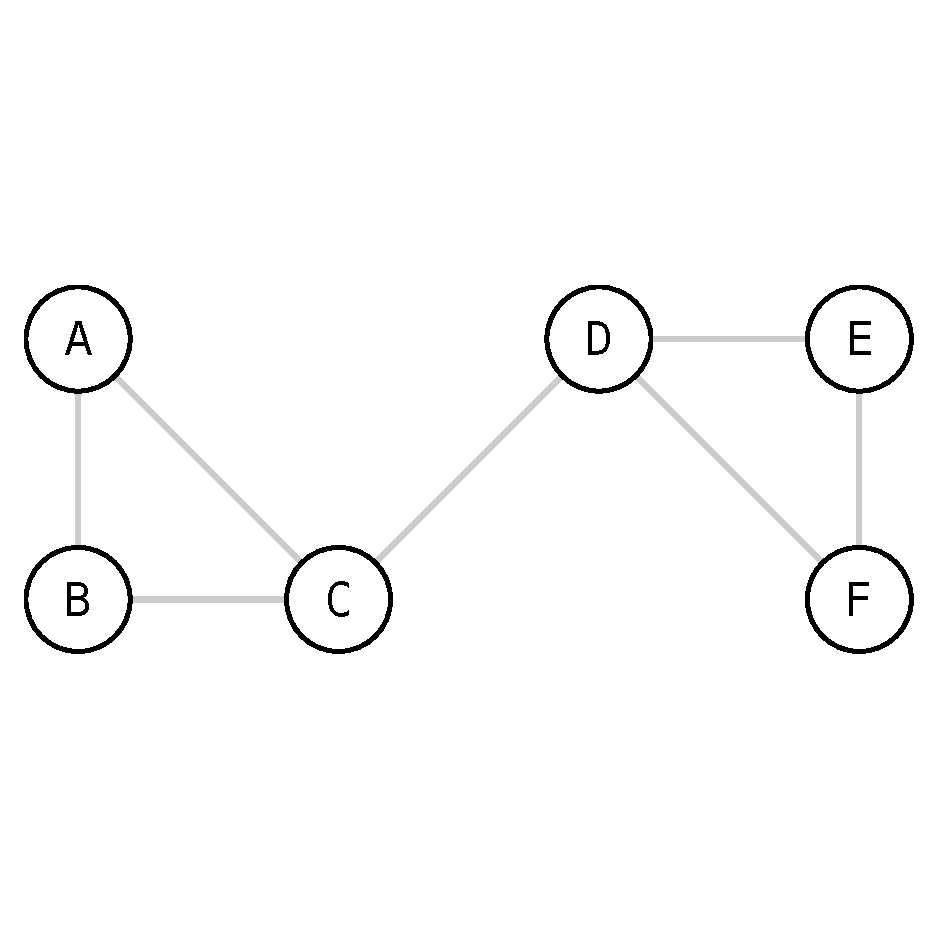
\includegraphics[width=0.46\textwidth]{python/lec04/bridges/bridges-0.pdf}\\[2pt]{\scriptsize Шаг 0. Исходный граф}} &
\shortstack{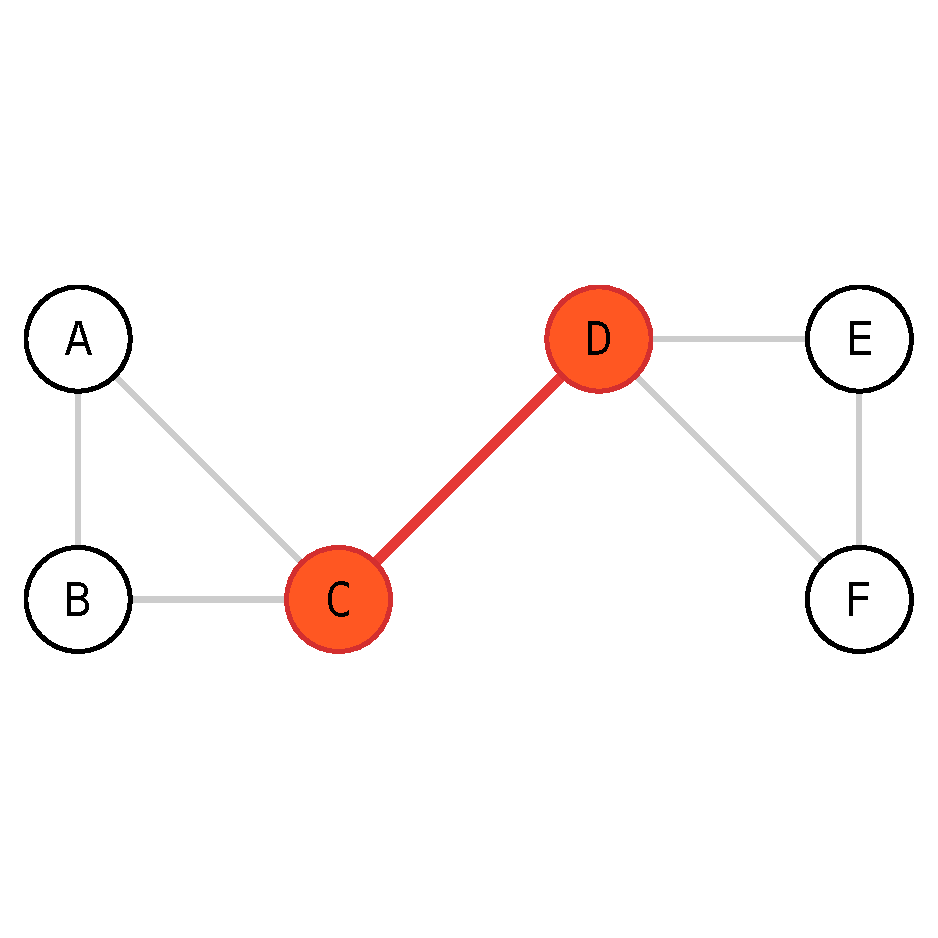
\includegraphics[width=0.46\textwidth]{python/lec04/bridges/bridges-1.pdf}\\[2pt]{\scriptsize Шаг 1. DFS из $A$: ориентируем рёбра по обходу}} \\
\end{tabular}\end{center}
\begin{center}\begin{tabular}{cc}
\shortstack{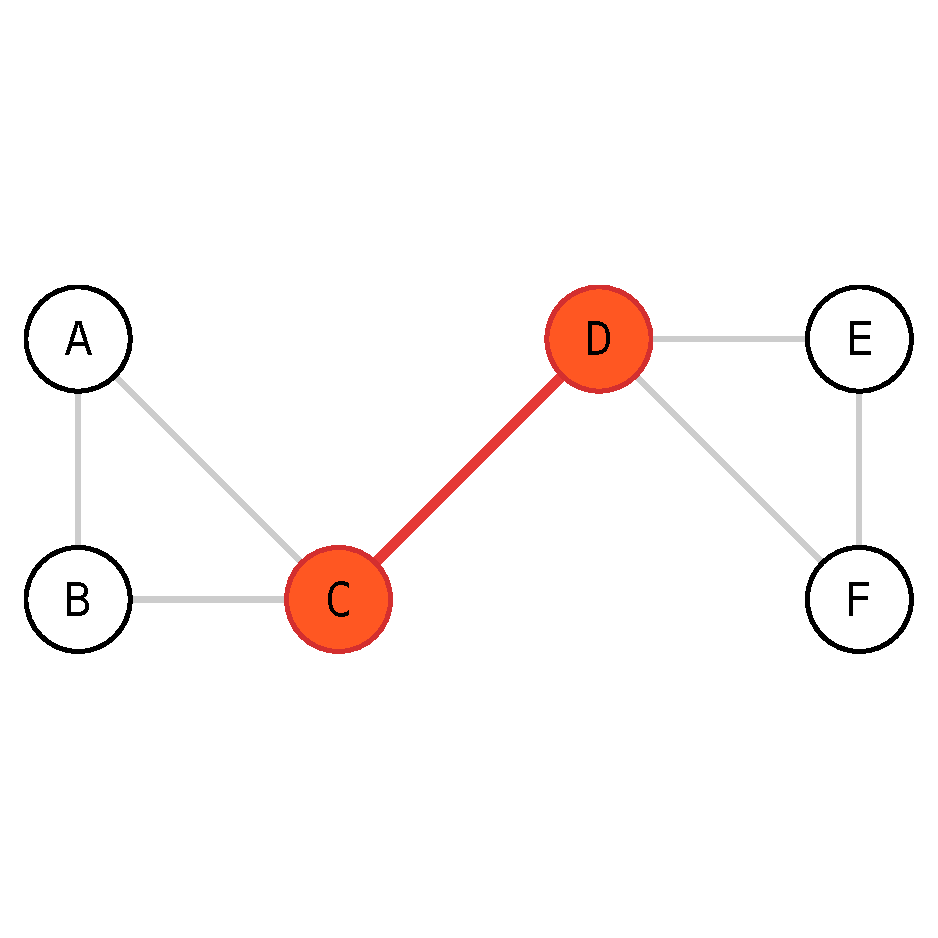
\includegraphics[width=0.46\textwidth]{python/lec04/bridges/bridges-2.pdf}\\[2pt]{\scriptsize Шаг 2. Инвертируем все рёбра}} &
\shortstack{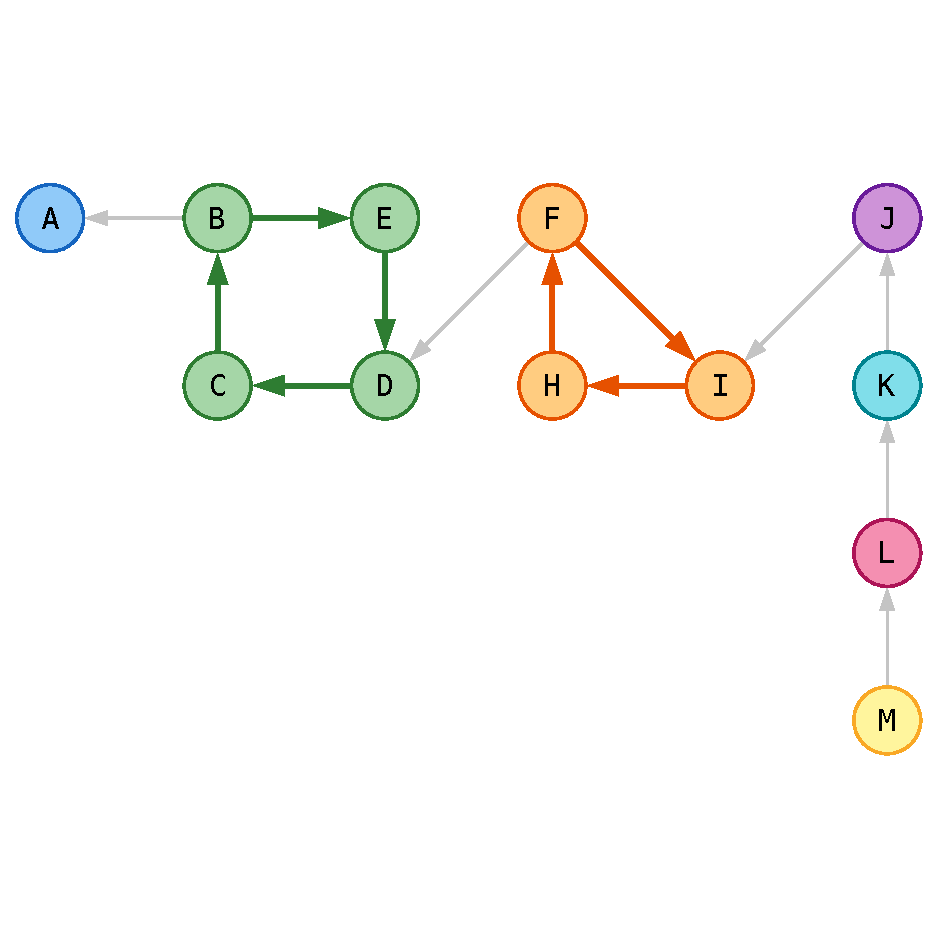
\includegraphics[width=0.46\textwidth]{python/lec04/bridges/bridges-3.pdf}\\[2pt]{\scriptsize Шаг 3. Серия DFS: компоненты --- цветами}} \\
\end{tabular}\end{center}
\begin{center}
\shortstack{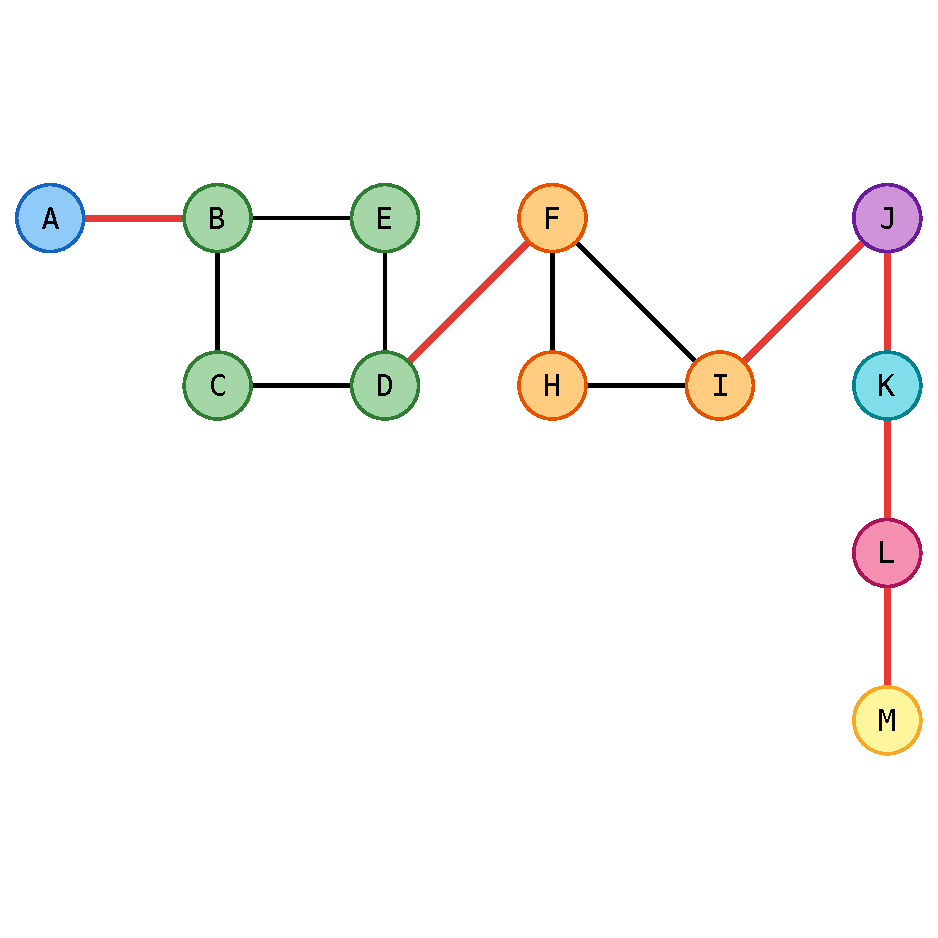
\includegraphics[width=0.5\textwidth]{python/lec04/bridges/bridges-4.pdf}\\[2pt]{\scriptsize Шаг 4. Мосты --- рёбра между разными цветами (красные)}}
\end{center}

\noindent\textit{Комментарии к шагам.} На шаге~1 поиск в глубину из $A$
ориентирует рёбра в порядке обхода:
$A{\to}B{\to}C{\to}D{\to}E$, ребро $E$--$B$ впервые посещается из $E$
(ориентируем $E \to B$); далее $D{\to}F{\to}H{\to}I{\to}J{\to}K{\to}L{\to}M$
и ребро $I \to F$. На шаге~3 серия DFS на инвертированном графе
(в порядке списка $A, B, C, \dots$) даёт компоненты
$\{A\}$, $\{B, C, D, E\}$, $\{F, H, I\}$, $\{J\}$, $\{K\}$, $\{L\}$,
$\{M\}$: из $A$ по инвертированным рёбрам никуда не попасть; из $B$
обходится цикл $B{\to}E{\to}D{\to}C{\to}B$; из $F$ --- цикл
$F{\to}I{\to}H{\to}F$; вершины $J, K, L, M$ остаются поодиночке.

\medskip
\textbf{Мосты данного графа} (рёбра между разными компонентами):
$A$--$B$,\; $D$--$F$,\; $I$--$J$,\; $J$--$K$,\; $K$--$L$,\; $L$--$M$.
\end{algo}


\chapter{Лекция 5. Слабая и сильная связность. Граф Герца. Эйлеровость}

% === Слабая и сильная связность ===

Ориентированный граф $G(V, E)$.

% Граф: p11-example-6.graph (два примера в одном файле)
\grfig{figures/p11-example-6.pdf}{Изотропия/анизотропия}

\textbf{Пример} (изотропия): неориент. дерево $A$--$B$--$C$--$D$, $C$--$E$ ---
достижимость \textit{не зависит} от направления рёбер.

\textbf{Пример} (анизотропия): $A \to B \to C$ ---
достижимость \textit{зависит} от направления рёбер.

\begin{defn}{Слабая связность}{weak-connectivity}
$G(V, E)$ --- ориентированный граф.

$G$ --- \textbf{слабо связен} $\;\Leftrightarrow\;$ $G$ связен без учёта ориентации рёбер.
\end{defn}

\begin{defn}{Сильная связность}{strong-connectivity}
$G(V, E)$ --- ориентированный граф.

$G$ --- \textbf{сильно связен} $\;\Leftrightarrow\;$
$\forall\, u, v \in V$: $\exists$ путь $u \to \ldots \to v$.
\end{defn}

\begin{defn}{Компонента сильной связности}{scc}
\textbf{Компонента сильной связности} --- максимальный по включению
сильно связный подграф.
\end{defn}

\bigskip
% === Пример: ориент. граф и его SCC ===
% Граф: p12-example-1.graph (ориентированный)
\grfig{figures/p12-example-1.pdf}{Ориент. граф (SCC) + граф Герца}
% Вершины: A, B, C, D, E, F, H, I, J
% Рёбра: A→B, B→D, D→A, B→C, C→E, C→H, H→I, I→J, J→H, E→F, F→E

\textbf{Пример.} Ориентированный граф:
$A \to B$,\; $B \to D$,\; $D \to A$ (цикл);
$B \to C$;\;
$C \to E$,\; $E \to F$,\; $F \to E$ (цикл);\;
$C \to H$,\; $H \to I$,\; $I \to J$,\; $J \to H$ (цикл).

Компоненты сильной связности:
$\{A, B, D\}$,\quad $\{C\}$,\quad $\{E, F\}$,\quad $\{H, I, J\}$.

\bigskip
% === Граф Герца ===
\begin{defn}{Граф Герца (конденсации)}{hertz-graph}
$G(V, E)$ --- орграф.

\textbf{Граф Герца} (граф конденсации) для $G$ ---
$\tilde{G}(\tilde{V}, \tilde{E})$, где:
\begin{itemize}
  \item $\tilde{V} \ni w \;\Leftrightarrow\; w$ --- компонента сильной связности $G$;
  \item $\tilde{e} \in \tilde{E} \;\Leftrightarrow\;$ между соответствующими
        компонентами сильной связности в $G$ $\exists$ путь.
\end{itemize}
\end{defn}

\textbf{Граф Герца} для примера выше:

$\{A,B,D\} \to \{C\}$,\quad
$\{C\} \to \{E,F\}$,\quad
$\{C\} \to \{H,I,J\}$.

% Граф Герца также изображён в p12-example-1.graph (нижняя часть)

\medskip
\textbf{Тривиальные свойства графа Герца:}
\begin{enumerate}
  \item $\forall\, G$:\; $\tilde{G}$ существует и единственен;
  \item $\tilde{G}$ --- строго ориентированный;
  \item $\tilde{G}$ --- ациклический.
\end{enumerate}

\bigskip
% === Алгоритм Косарайю ===
\begin{algo}{Алгоритм Косарайю (построение графа Герца)}{kosaraju}
Алгоритм для выделения компонент сильной связности.

\medskip
\textbf{Шаг I.} Серия DFS: <<тупиковая>> вершина (все исходящие рёбра
которой уже обработаны) кладётся в стек. Стек заполняется снизу вверх
по порядку завершения обработки вершин.

\textit{Зачем это нужно:} если из компоненты $X$ есть путь в компоненту
$Y$ ($X$ <<выше по течению>>), то хотя бы одна вершина $X$ окажется в
стеке \emph{выше} всех вершин $Y$. Поэтому на шаге~III обход стартует
из компонент, <<выше по течению>>, и не <<перетекает>> в чужие компоненты.

\textbf{Шаг II.} $\operatorname{inv} E$ --- инвертируем все рёбра.

\textbf{Шаг III.} Серия DFS, согласованная со стеком: достаём вершины
с верха стека; из каждой ещё не помеченной вершины запускаем DFS по
\emph{инвертированным} рёбрам --- все достижимые непомеченные вершины
образуют одну компоненту сильной связности (красим своим цветом).

\textbf{Результат:} компоненты сильной связности; стянув каждую в одну
вершину, получаем граф Герца.

\medskip
\noindent\textbf{Работа алгоритма по шагам} (граф из примера выше;
стек показан справа, верх стека --- сверху):

\begin{center}\begin{tabular}{cc}
\shortstack{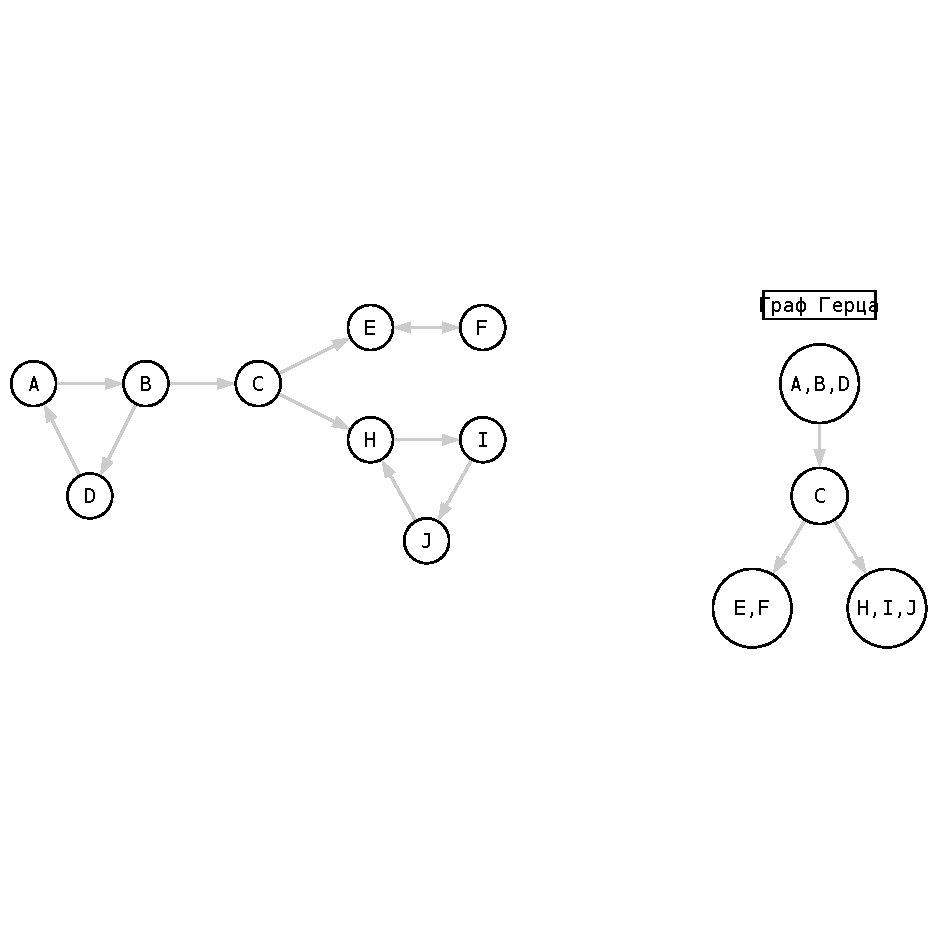
\includegraphics[width=0.46\textwidth]{python/lec05/kosaraju/kosaraju-0.pdf}\\[2pt]{\scriptsize Шаг 0. Исходный граф}} &
\shortstack{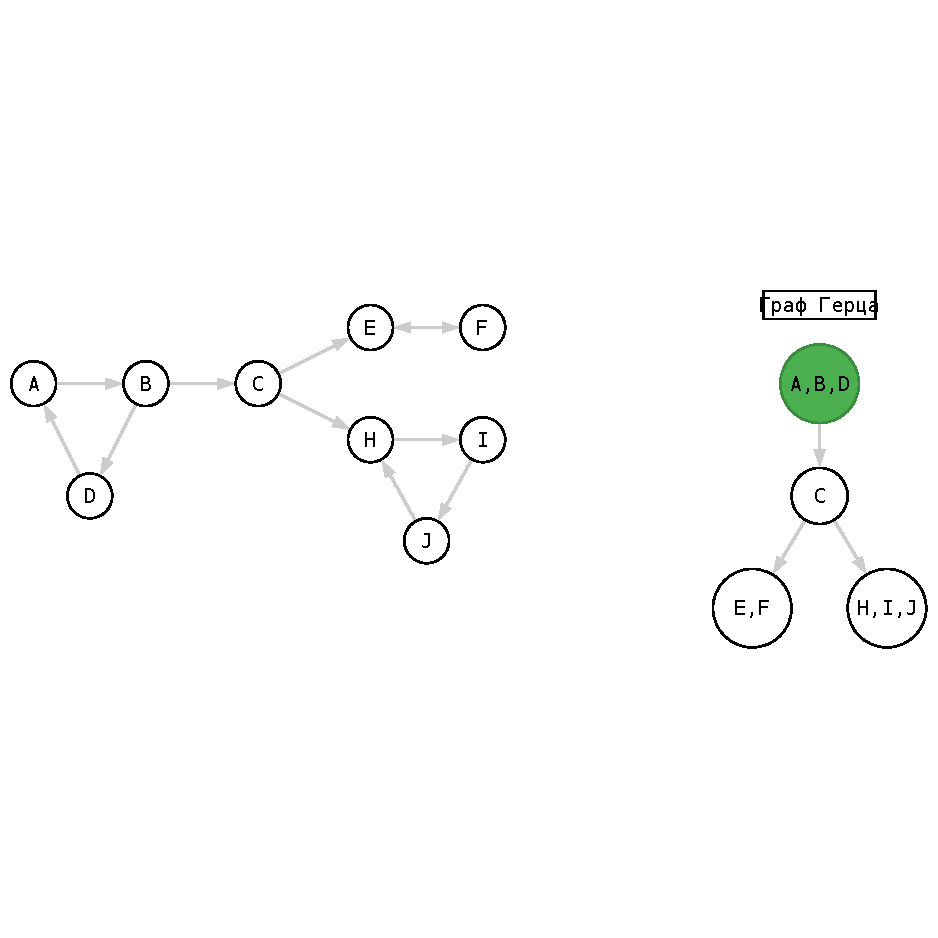
\includegraphics[width=0.46\textwidth]{python/lec05/kosaraju/kosaraju-1.pdf}\\[2pt]{\scriptsize Шаг 1. Серия DFS из $A$: стек по временам выхода}} \\
\end{tabular}\end{center}
\begin{center}\begin{tabular}{cc}
\shortstack{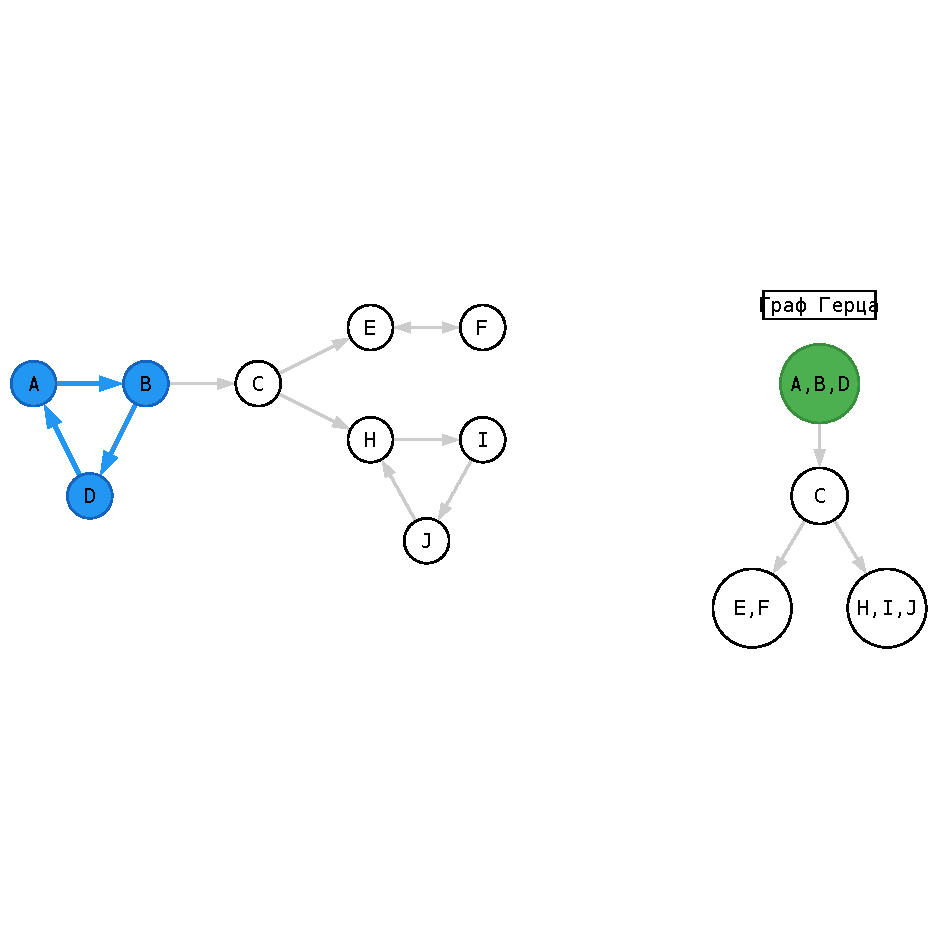
\includegraphics[width=0.46\textwidth]{python/lec05/kosaraju/kosaraju-2.pdf}\\[2pt]{\scriptsize Шаг 2. Инвертируем все рёбра}} &
\shortstack{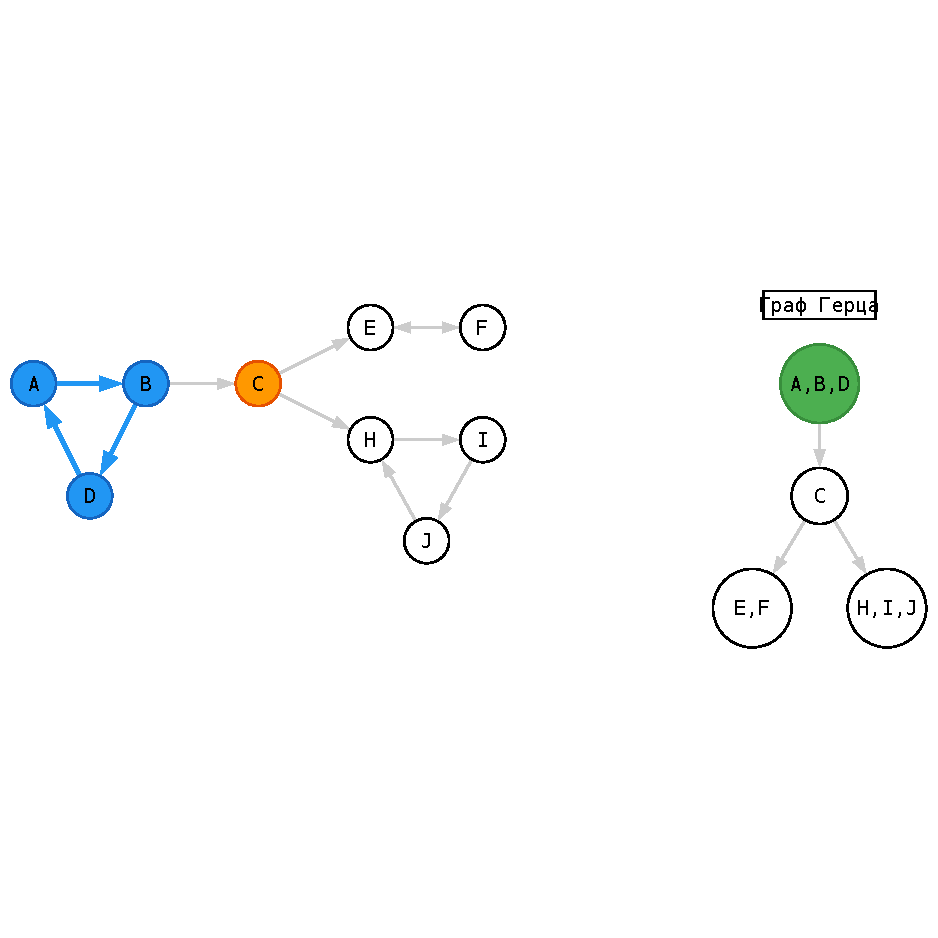
\includegraphics[width=0.46\textwidth]{python/lec05/kosaraju/kosaraju-3.pdf}\\[2pt]{\scriptsize Шаг 3. Сверху стека $A$: DFS даёт $\{A, D, B\}$}} \\
\end{tabular}\end{center}
\begin{center}\begin{tabular}{cc}
\shortstack{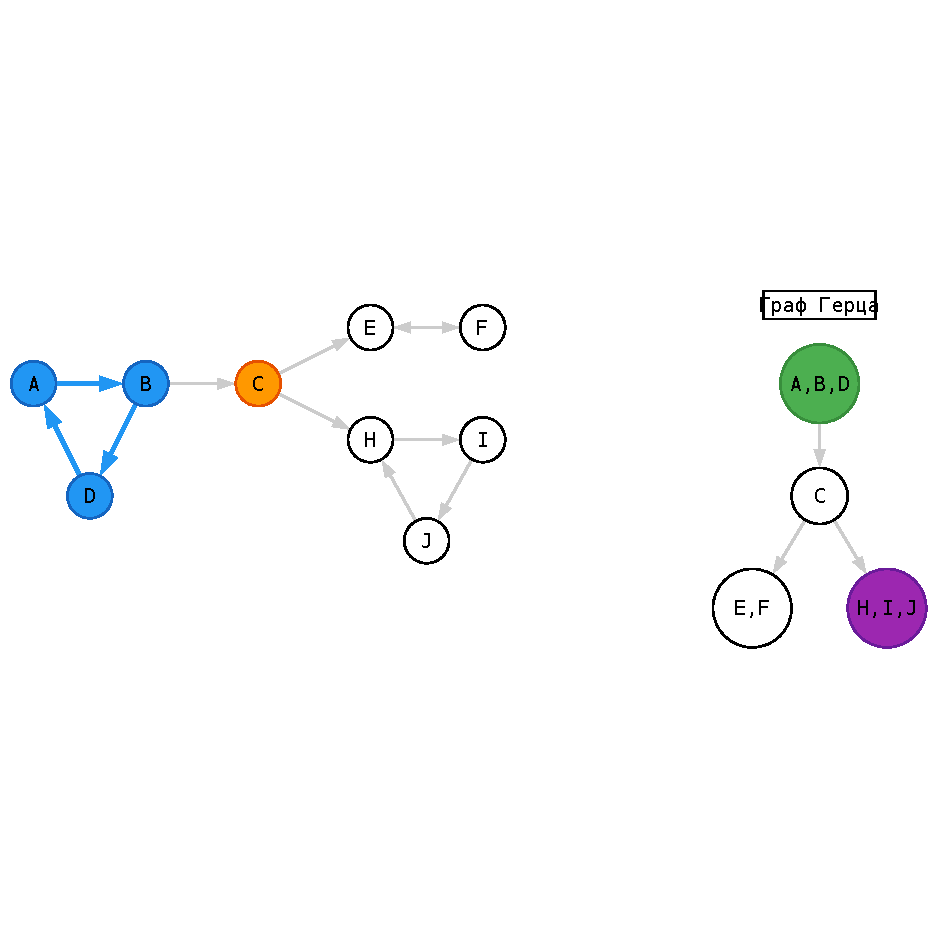
\includegraphics[width=0.46\textwidth]{python/lec05/kosaraju/kosaraju-4.pdf}\\[2pt]{\scriptsize Шаг 4. Следующая непомеченная $C$: $\{C\}$}} &
\shortstack{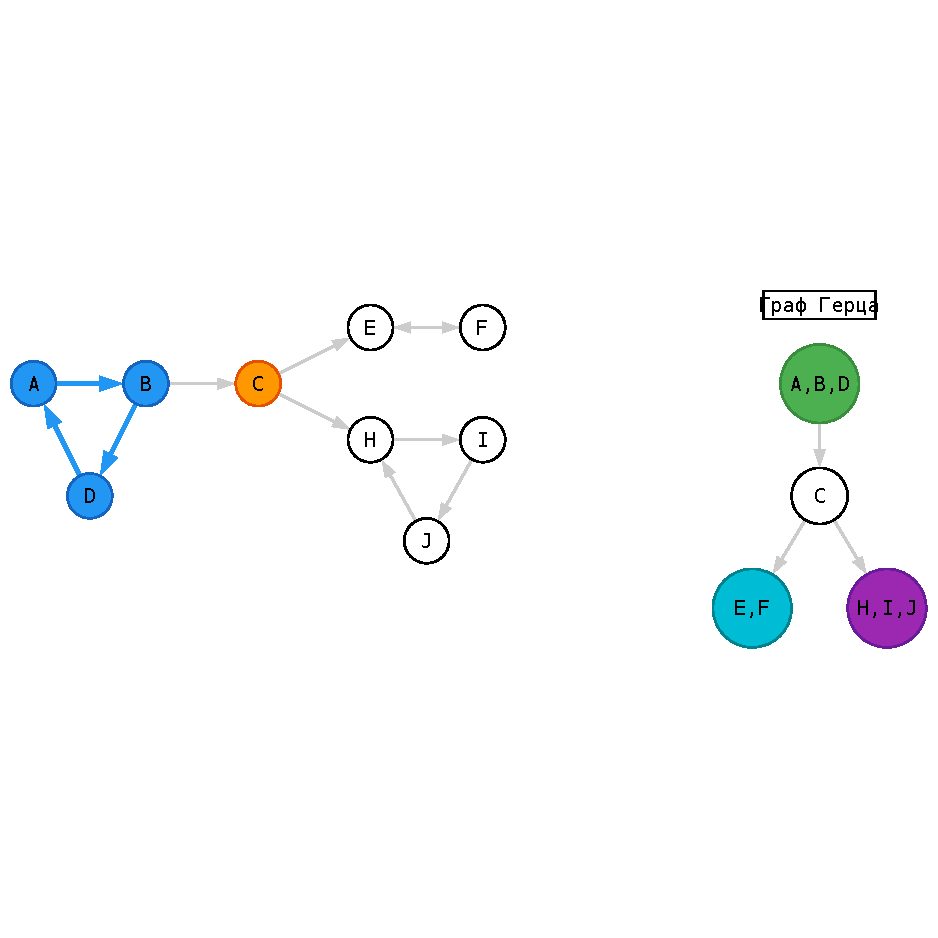
\includegraphics[width=0.46\textwidth]{python/lec05/kosaraju/kosaraju-5.pdf}\\[2pt]{\scriptsize Шаг 5. Из $H$: компонента $\{H, J, I\}$}} \\
\end{tabular}\end{center}
\begin{center}\begin{tabular}{cc}
\shortstack{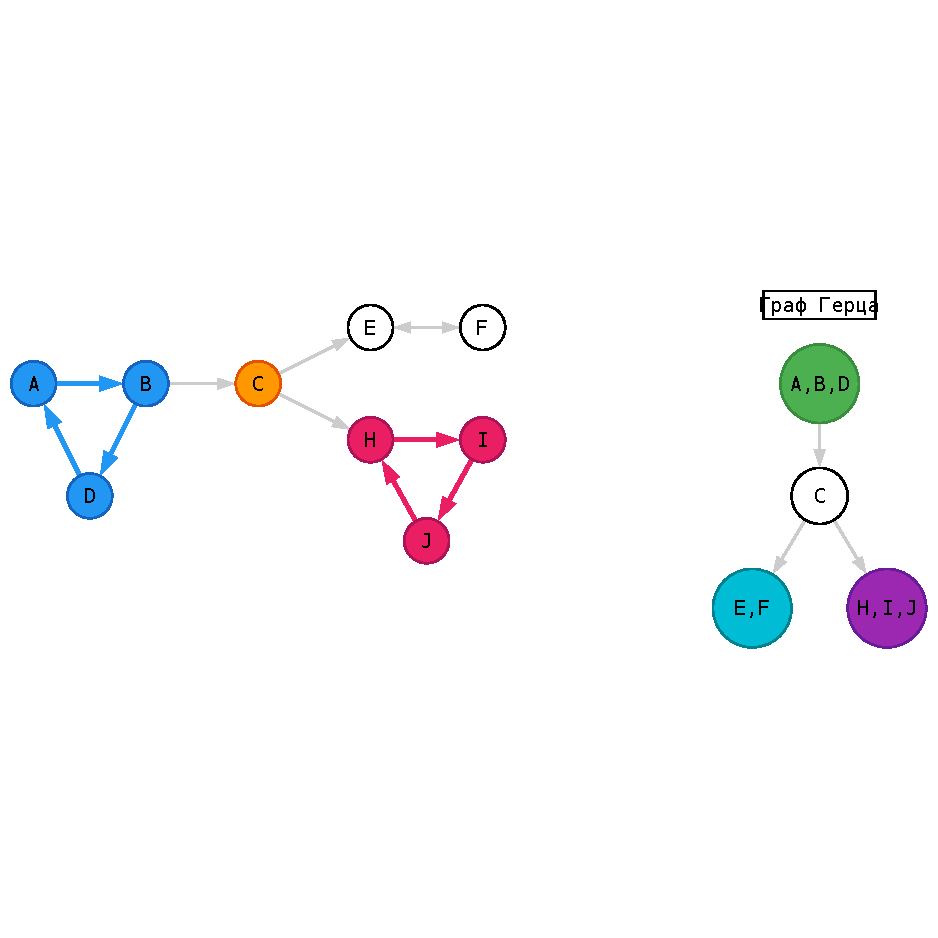
\includegraphics[width=0.46\textwidth]{python/lec05/kosaraju/kosaraju-6.pdf}\\[2pt]{\scriptsize Шаг 6. Из $E$: компонента $\{E, F\}$}} &
\shortstack{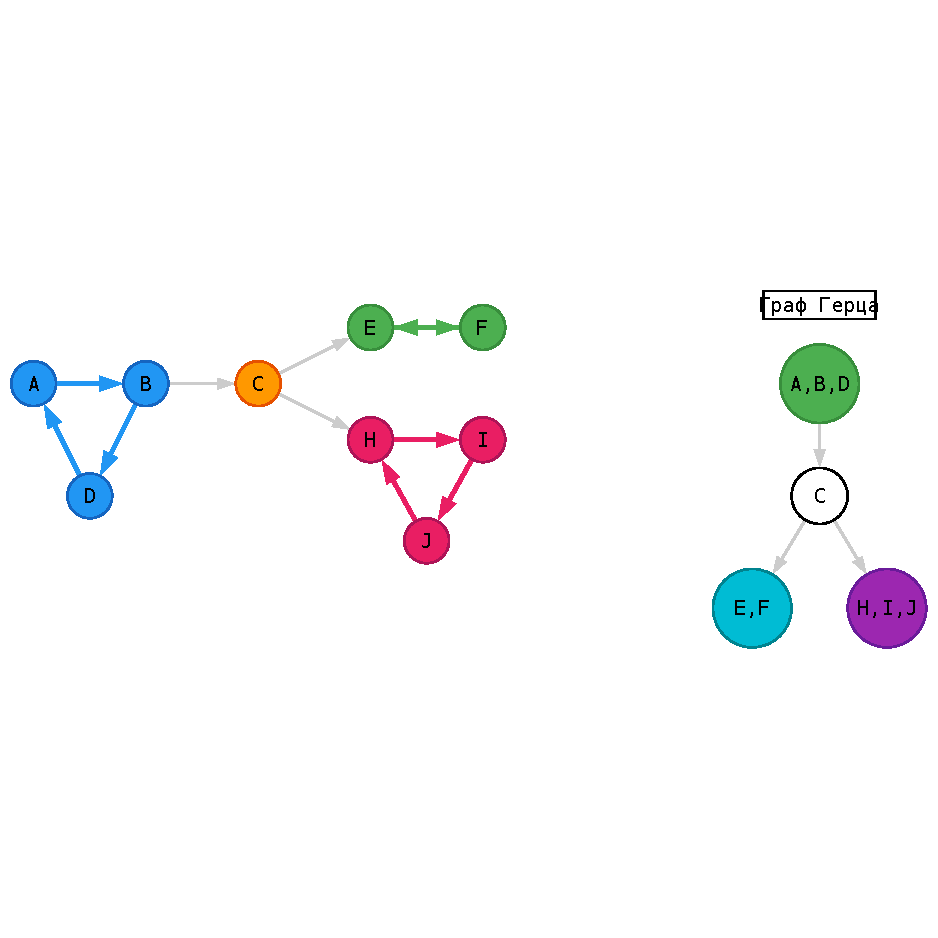
\includegraphics[width=0.46\textwidth]{python/lec05/kosaraju/kosaraju-7.pdf}\\[2pt]{\scriptsize Шаг 7. Итог: 4 компоненты сильной связности}} \\
\end{tabular}\end{center}

\noindent\textit{Комментарии к шагам.} На шаге~1 поиск в глубину из $A$
обходит граф: $A \to B \to D$ (ребро $D \to A$ ведёт в посещённую
вершину, $D$ --- тупиковая, кладём в стек); далее $B \to C \to E \to F$
(ребро $F \to E$ --- в посещённую, $F$ в стек, затем $E$);
$C \to H \to I \to J$ ($J \to H$ --- в посещённую, в стек уходят
$J$, $I$, $H$); наконец в стек уходят $C$, $B$, $A$. Стек снизу вверх:
$D, F, E, J, I, H, C, B, A$.

На шаге~III достаём вершины сверху: из $A$ по инвертированным рёбрам
достижимы $D$ и $B$ --- компонента $\{A, B, D\}$ (шаг~3); $B$ уже
помечена, следующая $C$ --- из неё по инвертированным рёбрам можно
попасть только в помеченную $B$, компонента $\{C\}$ (шаг~4); из $H$
достижимы $J$ и $I$ --- $\{H, I, J\}$ (шаг~5); из $E$ достижима $F$ ---
$\{E, F\}$ (шаг~6). Все вершины помечены --- алгоритм завершён (шаг~7).
\end{algo}

% ============================================================
% ЭЙЛЕРОВОСТЬ (стр. 13, dir2 стр. 1)
% ============================================================

\subsection*{Эйлеровость}

\begin{defn}{Эйлеров цикл и эйлеров путь}{euler}
Дан $G(V, E)$.

$G$ содержит \textbf{эйлеров цикл} $\;\Leftrightarrow\;$ $\exists$ в $G$ цикл, содержащий
$\forall\, e \in E$ ровно 1 раз.

$G$ содержит \textbf{эйлеров путь} $\;\Leftrightarrow\;$ в $G$ $\exists$ открытый простой
путь, содержащий $\forall\, e \in E$.
\end{defn}

\begin{defn}{Эйлеров граф}{euler-graph}
$G$ --- \textbf{эйлеров}:
\begin{itemize}
  \item $G$ --- ориент. $\;\Leftrightarrow\;$ в $G$ $\exists$ эйлеров цикл, $G$ --- слабо связен.
  \item $G$ --- неориент. $\;\Leftrightarrow\;$ в $G$ $\exists$ эйлеров цикл, $G$ --- связный.
\end{itemize}
\end{defn}

\begin{defn}{Полуэйлеров граф}{semi-euler-graph}
$G$ --- \textbf{полуэйлеров}:
\begin{itemize}
  \item $G$ --- ориент. $\;\Leftrightarrow\;$ в $G$ $\exists$ эйлеров путь, $G$ --- слабо связен.
  \item $G$ --- неориент. $\;\Leftrightarrow\;$ в $G$ $\exists$ эйлеров путь, $G$ --- связный.
\end{itemize}
\end{defn}

\medskip
\noindent\textbf{Примеры} (проверяем по степеням вершин):

% Пример 1: треугольник — Э
% Граф: p13-example-1.graph
\grfig{figures/p13-example-1.pdf}{Эйлеровость: пример 1 --- эйлеров}
\noindent\textit{Пример 1.} Цикл $1$--$2$--$3$--$1$: все степени равны $2$
(чётные), граф связный $\Rightarrow$ \textbf{эйлеров}; эйлеров цикл --- сам
треугольник.

% Пример 2: неориент. путь 1--2--3--4 — ПЭ
% Граф: p13-example-2.graph
\grfig{figures/p13-example-2.pdf}{Эйлеровость: пример 2 --- полуэйлеров}
\noindent\textit{Пример 2.} Цепь $1$--$2$--$3$--$4$: ровно две вершины
нечётной степени ($\deg 1 = \deg 4 = 1$), у остальных степень $2$
$\Rightarrow$ \textbf{полуэйлеров}; эйлеров путь --- сама цепь от $1$ до $4$.

% Пример 3: треугольник + два «уса» — ПЭ
% Граф: p13-example-3.graph
\grfig{figures/p13-example-3.pdf}{Эйлеровость: пример 3 --- полуэйлеров}
\noindent\textit{Пример 3.} Треугольник $1$--$2$--$3$ с <<усами>> $3$--$4$ и
$3$--$5$: нечётные степени ровно у двух вершин --- $\deg 4 = \deg 5 = 1$
(при этом $\deg 3 = 4$, $\deg 1 = \deg 2 = 2$) $\Rightarrow$
\textbf{полуэйлеров}; эйлеров путь, например, $4$--$3$--$1$--$2$--$3$--$5$.

% Пример 4: четыре вершины нечётной степени — ни Э, ни ПЭ
% Граф: p13-example-4.graph
\grfig{figures/p13-example-4.pdf}{Эйлеровость: пример 4 --- ни Э, ни ПЭ}
\noindent\textit{Пример 4.} Треугольник $1$--$2$--$3$ с <<усами>> $3$--$4$ и
$5$--$2$: нечётная степень у \emph{четырёх} вершин
($\deg 2 = \deg 3 = 3$, $\deg 4 = \deg 5 = 1$) $\Rightarrow$
\textbf{ни эйлеров, ни полуэйлеров}.

% Пример 5: все степени чётные — Э
% Граф: p13-example-5.graph
\grfig{figures/p13-example-5.pdf}{Эйлеровость: пример 5 --- эйлеров}
\noindent\textit{Пример 5.} Два цикла $1$--$2$--$3$--$1$ и
$2$--$4$--$5$--$2$ с общей вершиной $2$: все степени чётные
($\deg 2 = 4$, у остальных $2$), граф связный $\Rightarrow$
\textbf{эйлеров}; эйлеров цикл: $1$--$2$--$4$--$5$--$2$--$3$--$1$.

% Пример 6: K4 — ни Э, ни ПЭ
% Граф: p13-example-6.graph
\grfig{figures/p13-example-6.pdf}{Эйлеровость: пример 6 --- ни Э, ни ПЭ}
\noindent\textit{Пример 6.} Полный граф $K_4$: \emph{все четыре} вершины
имеют нечётную степень $3$ $\Rightarrow$ \textbf{ни эйлеров, ни
полуэйлеров}.

\begin{statement}{Критерий Э и ПЭ}{euler-criterion}

\textbf{I.} $G(V,E)$ --- неориент., связный.

\begin{enumerate}[label=\alph*)]
  \item $G$ --- Э $\;\Leftrightarrow\;$ $\forall\, v \in V$: $\deg(v) \vdots\; 2$
  \item $G$ --- ПЭ $\;\Leftrightarrow\;$ $\exists\, u \neq v \in V$: $\deg(u) \ndiv 2$,\; $\deg(v) \ndiv 2$, \\
        $\forall\, w \in V \setminus \{u, v\}$: $\deg(w) \vdots\; 2$
\end{enumerate}

\textbf{II.} $G$ --- ориент., связный (слабо).

\begin{enumerate}[label=\alph*)]
  \item $G$ --- Э $\;\Leftrightarrow\;$ $\forall\, v \in V$: $\delta^+(v) = \delta^-(v)$
  \item $G$ --- ПЭ $\;\Leftrightarrow\;$ $\exists\, u, v \in V$:
        $\delta^+(u) = \delta^-(u) + 1$,\;
        $\delta^-(v) = \delta^+(v) + 1$, \\
        $\forall\, w \in V \setminus \{u, v\}$: $\delta^+(w) = \delta^-(w)$
\end{enumerate}
\end{statement}

\begin{proof}[Доказательство (случай I)]
\textbf{a) Необходимость ($\Rightarrow$).} Пусть в $G$ есть эйлеров цикл.
Идя по циклу, мы в каждую вершину столько же раз <<входим>>, сколько
<<выходим>>, и каждое инцидентное вершине ребро используется ровно один
раз --- либо для входа, либо для выхода. Значит, рёбра при каждой вершине
разбиваются на пары <<вход--выход>>, и все степени чётны.

\textbf{a) Достаточность ($\Leftarrow$).} Пусть все степени чётны и $G$
связен; индукция по числу рёбер. Возьмём любую вершину $v_0$ и пойдём по
непройденным рёбрам, никогда не останавливаясь: войдя в вершину
$w \ne v_0$, мы заняли нечётное число её рёбер, а степень чётна --- значит,
есть свободное ребро для выхода. Застрять можно только в $v_0$, т.\,е.
получаем цикл $C$. Удалим рёбра $C$ из графа: степени снова чётны
(в каждой вершине цикл занял чётное число рёбер). Каждая компонента
оставшегося графа по предположению индукции имеет эйлеров цикл, причём
из связности $G$ каждая компонента пересекается с $C$ по вершине.
Вклеим эти циклы в $C$ при прохождении общих вершин --- получим эйлеров
цикл всего графа.

\textbf{b)} Сводится к пункту a): если ровно две вершины $u, v$ нечётны,
добавим фиктивное ребро $u$--$v$ --- все степени станут чётными, по
пункту a) существует эйлеров цикл; удалив из него фиктивное ребро,
получим эйлеров путь из $u$ в $v$. Обратно: эйлеров путь из $u$ в $v$
плюс фиктивное ребро $u$--$v$ дают эйлеров цикл, поэтому по пункту a)
все вершины, кроме $u$ и $v$, чётны, а $u$ и $v$ нечётны.

Случай II (ориентированный) доказывается дословно так же с заменой
степени на полустепени: внутри цикла в каждую вершину входим столько же
раз, сколько выходим, поэтому $\delta^+(v) = \delta^-(v)$, и наоборот.
\end{proof}

% ============================================================
% Алгоритм Флёри (стр. 14, dir2 стр. 2)
% ============================================================

\medskip
\textbf{Алгоритм поиска эйлерова пути / эйлерова цикла} (не единственные!).

\begin{algo}{Алгоритм Флёри}{fleury}
\textbf{Вход:} $G$ --- Э или ПЭ.

\textbf{Выход:} эйлеров цикл / эйлеров путь.

\medskip
\textbf{P.S.} Граф не может быть Э и ПЭ одновременно.

\medskip
\textbf{Инициализация:}
\begin{enumerate}
  \item Э $\;\Rightarrow\;$ $\operatorname{start} \in V$ --- любая вершина.
  \item ПЭ $\;\Rightarrow\;$ $\operatorname{start} \in V$: $\deg(v) \ndiv 2$.
  \item (ориент.) $\;\Rightarrow\;$ $\operatorname{start} \in V$: $\delta^-(v) = \delta^+(v) + 1$.
\end{enumerate}

\medskip
\textbf{Шаг (step):}
на каждом шаге идём по ребру, которое \textbf{не является мостом}
в оставшемся графе (если есть выбор). По мосту идём, только когда
другого ребра из текущей вершины нет. Пройденное ребро удаляем.

\medskip
\noindent\textbf{Пример.}
% Граф: p14-example-1.graph
\grfig[0.5]{figures/p14-example-1.pdf}{Алг. Флёри: пример графа}
Степени: $\deg A = \deg C = \deg E = 4$, $\deg B = \deg D = 3$ ---
ровно две нечётные вершины, граф полуэйлеров; стартуем из нечётной
вершины $B$ (закончим в $D$).

\medskip
\begin{center}
\begin{tabular}{c|c|c|l}
№ & вершина & ребро & комментарий (мосты в оставшемся графе) \\ \hline
1 & $B$ & $B$--$A$ & мостов нет, берём любое ребро \\
2 & $A$ & $A$--$C$ & мостов нет \\
3 & $C$ & $C$--$B$ & мостов нет \\
4 & $B$ & $B$--$E$ & единственное оставшееся ребро из $B$ \\
5 & $E$ & $E$--$C$ & $E$--$C$ не мост (цикл $C$--$D$--$E$ цел) \\
6 & $C$ & $C$--$D$ & единственное ребро из $C$ (мост, но выбора нет) \\
7 & $D$ & $D$--$E$ & $D$--$E$ не мост, а $D$--$A$ --- мост: избегаем \\
8 & $E$ & $E$--$A$ & единственное ребро из $E$ \\
9 & $A$ & $A$--$D$ & последнее ребро; финиш в $D$ \\
\end{tabular}
\end{center}

\medskip
Эйлеров путь: $B, A, C, B, E, C, D, E, A, D$ --- все $9$ рёбер ровно
по одному разу, от одной нечётной вершины ($B$) до другой ($D$).

\medskip
\noindent\textbf{Работа алгоритма по шагам} (номера на рёбрах ---
порядок прохождения; старт $B$ --- синий, текущая вершина --- оранжевая):

\begin{center}\begin{tabular}{cc}
\shortstack{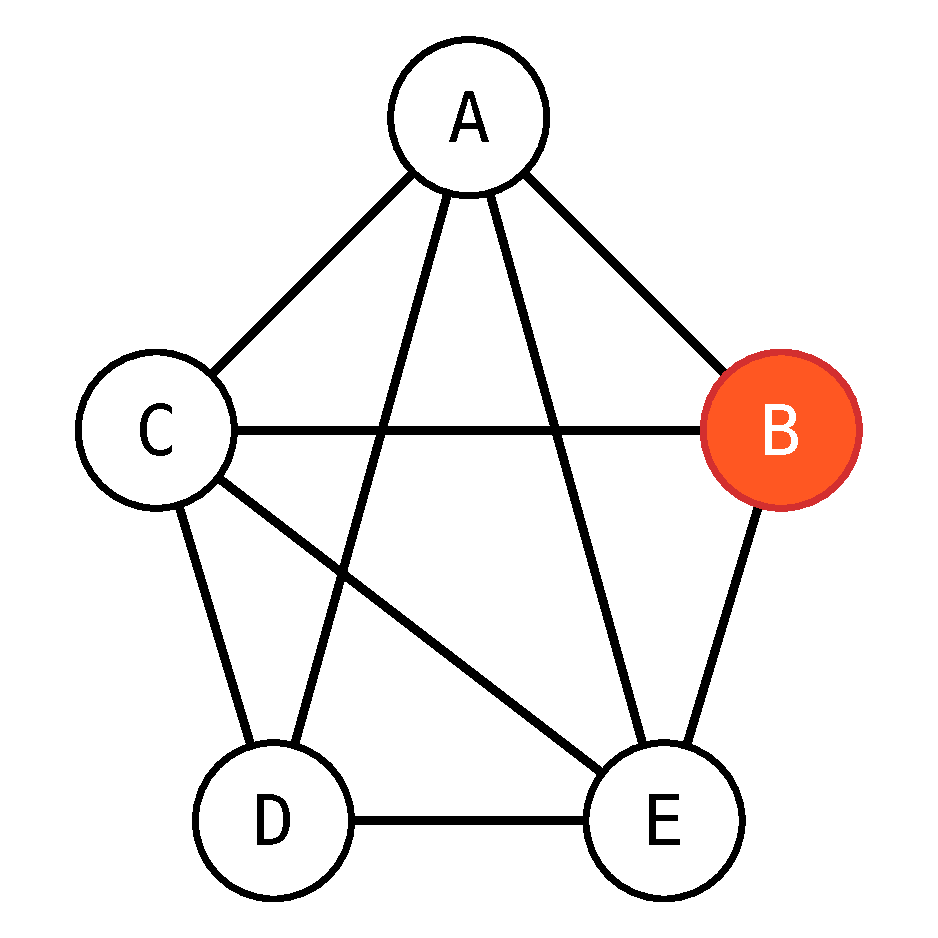
\includegraphics[width=0.40\textwidth]{python/lec05/fleury/fleury-0.pdf}\\[2pt]{\scriptsize Шаг 0. Старт в нечётной вершине $B$}} &
\shortstack{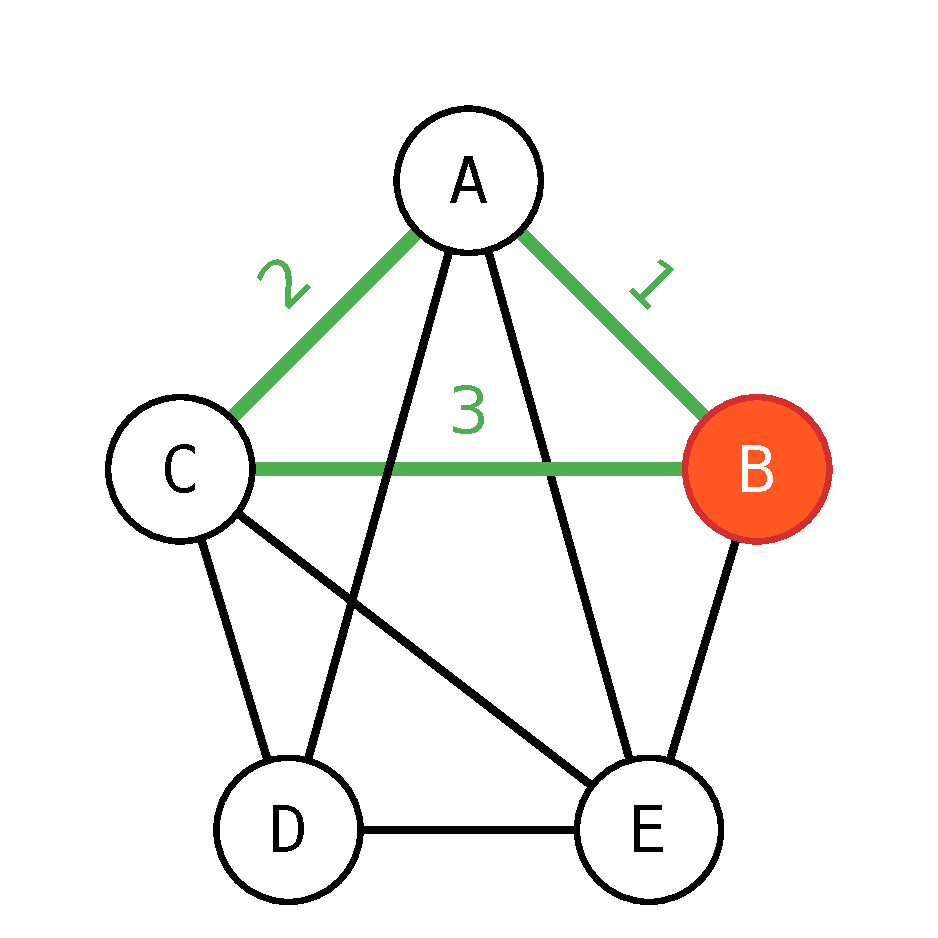
\includegraphics[width=0.40\textwidth]{python/lec05/fleury/fleury-1.pdf}\\[2pt]{\scriptsize Шаги 1--3: $B$--$A$--$C$--$B$}} \\
\end{tabular}\end{center}
\begin{center}\begin{tabular}{cc}
\shortstack{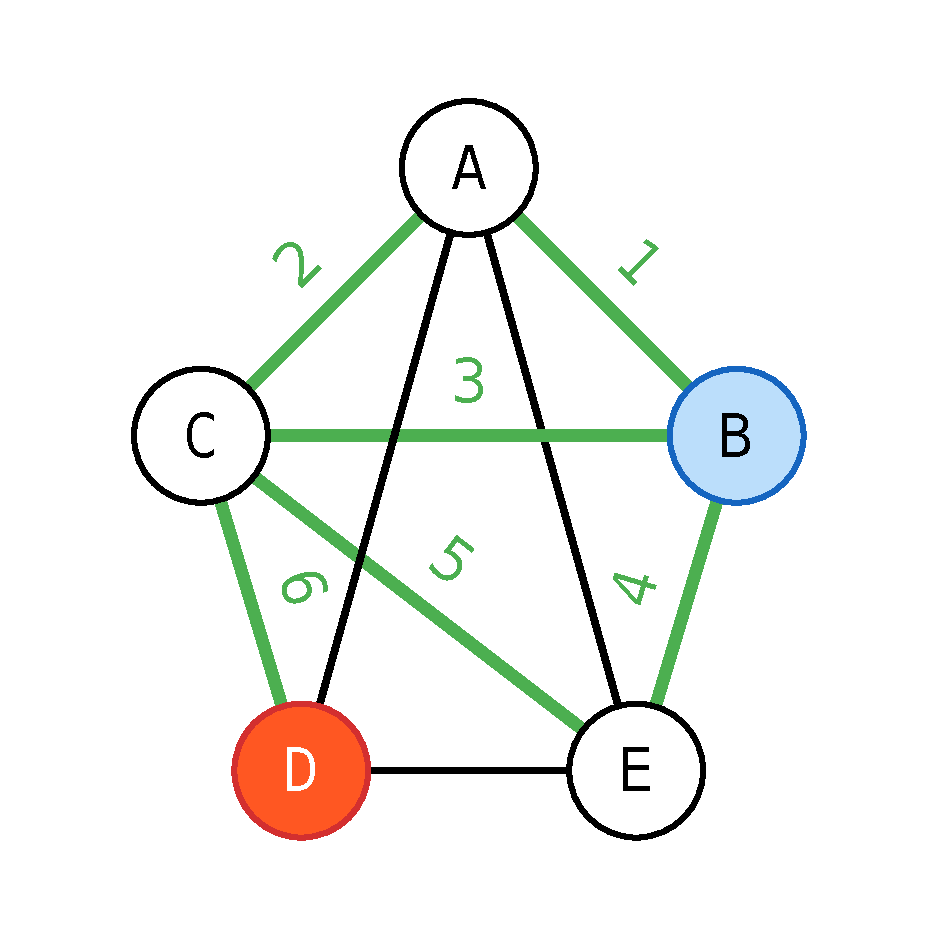
\includegraphics[width=0.40\textwidth]{python/lec05/fleury/fleury-2.pdf}\\[2pt]{\scriptsize Шаги 4--6: $B$--$E$--$C$--$D$}} &
\shortstack{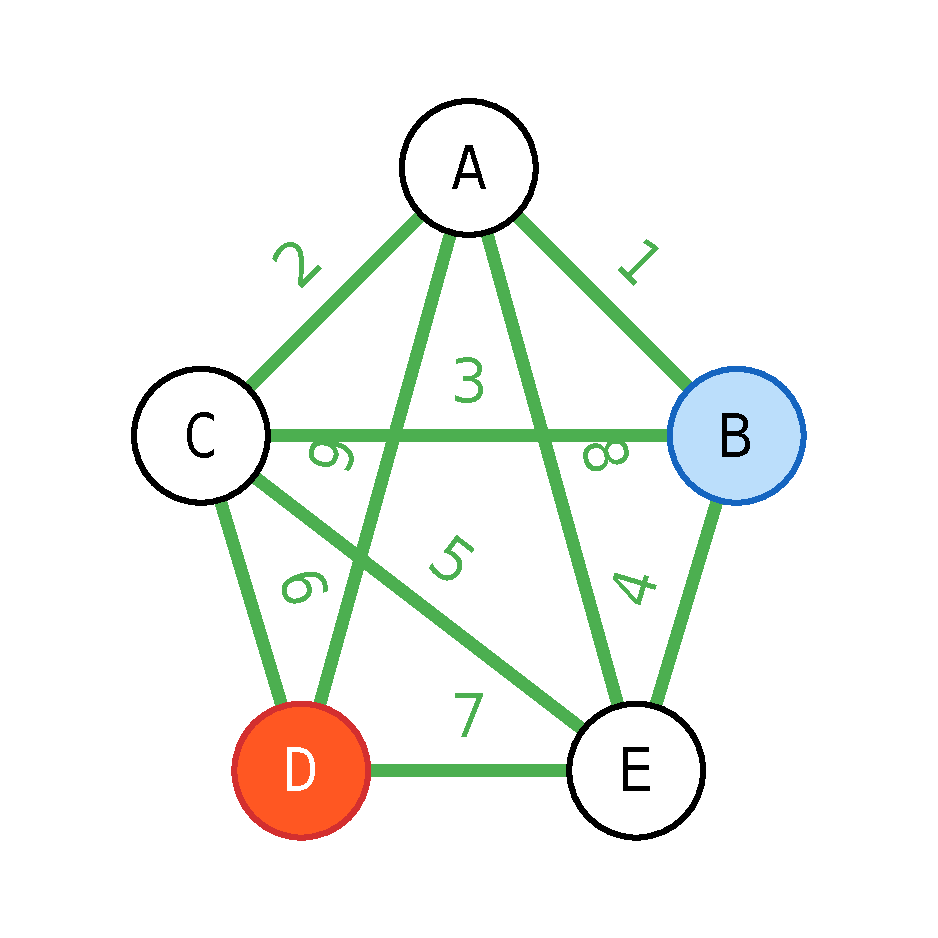
\includegraphics[width=0.40\textwidth]{python/lec05/fleury/fleury-3.pdf}\\[2pt]{\scriptsize Шаги 7--9: $D$--$E$--$A$--$D$, финиш в $D$}} \\
\end{tabular}\end{center}
\end{algo}

% ============================================================
% Алгоритм (на списках инцидентности) — стр. 14
% ============================================================

\begin{algo}{Алгоритм поиска эйлерова цикла (на списках инцидентности)}{euler-incidence}
\textbf{Идея.} Граф задан списками инцидентности (для каждой вершины ---
список исходящих рёбер). Используются стек \texttt{temp} и список
\texttt{result}:

\begin{enumerate}
  \item кладём стартовую вершину в стек;
  \item пока стек не пуст, смотрим на вершину $v$ с верха стека:
  \begin{itemize}
    \item если в списке $v$ осталось неиспользованное ребро $v \to u$ ---
          вычёркиваем его из списка и кладём $u$ в стек;
    \item если список $v$ исчерпан --- снимаем $v$ со стека и дописываем
          её в \texttt{result};
  \end{itemize}
  \item в конце \texttt{result}, прочитанный \emph{в обратном порядке},
        --- эйлеров цикл (путь).
\end{enumerate}

\medskip
\noindent\textbf{Пример.}
% Граф: p14-example-2.graph
\grfig[0.5]{figures/p14-example-2.pdf}{Алг. на списках инцидентности}
% Дуги: A→B, B→C, D→C, A→D, E→D, K→E, D→K, C→A, C→E, E→C

Полустепени: у вершины $A$ выходов на один больше, чем входов
($\delta^- (A) = 2$, $\delta^+(A) = 1$), у $C$ --- наоборот
($\delta^-(C) = 2$, $\delta^+(C) = 3$), у остальных входы равны выходам
--- по критерию граф полуэйлеров; эйлеров путь идёт из $A$ в $C$.

\medskip
\noindent Списки инцидентности (исходящие рёбра):

\begin{center}
\begin{tabular}{ll}
$A$: & $B,\; D$ \\
$B$: & $C$ \\
$C$: & $A,\; E$ \\
$D$: & $C,\; K$ \\
$E$: & $D,\; C$ \\
$K$: & $E$ \\
\end{tabular}
\end{center}

\medskip
\noindent Работа алгоритма: сначала стек только растёт ---
$A \to B \to C \to A \to D \to C \to E \to D \to K \to E \to C$ (каждый
раз вычёркиваем первое неиспользованное ребро из списка текущей вершины).
К этому моменту все $10$ рёбер израсходованы, и стек начинает
разбираться: вершины по очереди исчерпаны и уходят в \texttt{result}.

\medskip
\noindent Состояния (\texttt{temp} --- стек после фазы роста, читается
снизу вверх; \texttt{result} --- порядок выгрузки, сверху вниз):

\medskip
\begin{center}
\begin{tabular}{c|c}
\textbf{temp} (низ $\to$ верх) & \textbf{result} \\ \hline
$A$ & $C$ \\
$B$ & $E$ \\
$C$ & $K$ \\
$A$ & $D$ \\
$D$ & $E$ \\
$C$ & $C$ \\
$E$ & $D$ \\
$D$ & $A$ \\
$K$ & $C$ \\
$E$ & $B$ \\
$C$ & $A$ \\
\end{tabular}
\end{center}

\medskip
Эйлеров путь --- это \texttt{result}, прочитанный снизу вверх:
\[
  A,\; B,\; C,\; A,\; D,\; C,\; E,\; D,\; K,\; E,\; C
\]
--- все $10$ дуг ровно по одному разу, из $A$ в $C$.
\end{algo}

% ============================================================
\begin{task}{Эйлеровость графа}{euler-task}
\textbf{Условие.} Дан связный граф на вершинах $A,B,C,D$ с рёбрами
$AB,\ BC,\ CD,\ DA,\ AC$. Выясните, является ли он эйлеровым или
полуэйлеровым, и при возможности укажите эйлеров путь/цикл.

\begin{center}
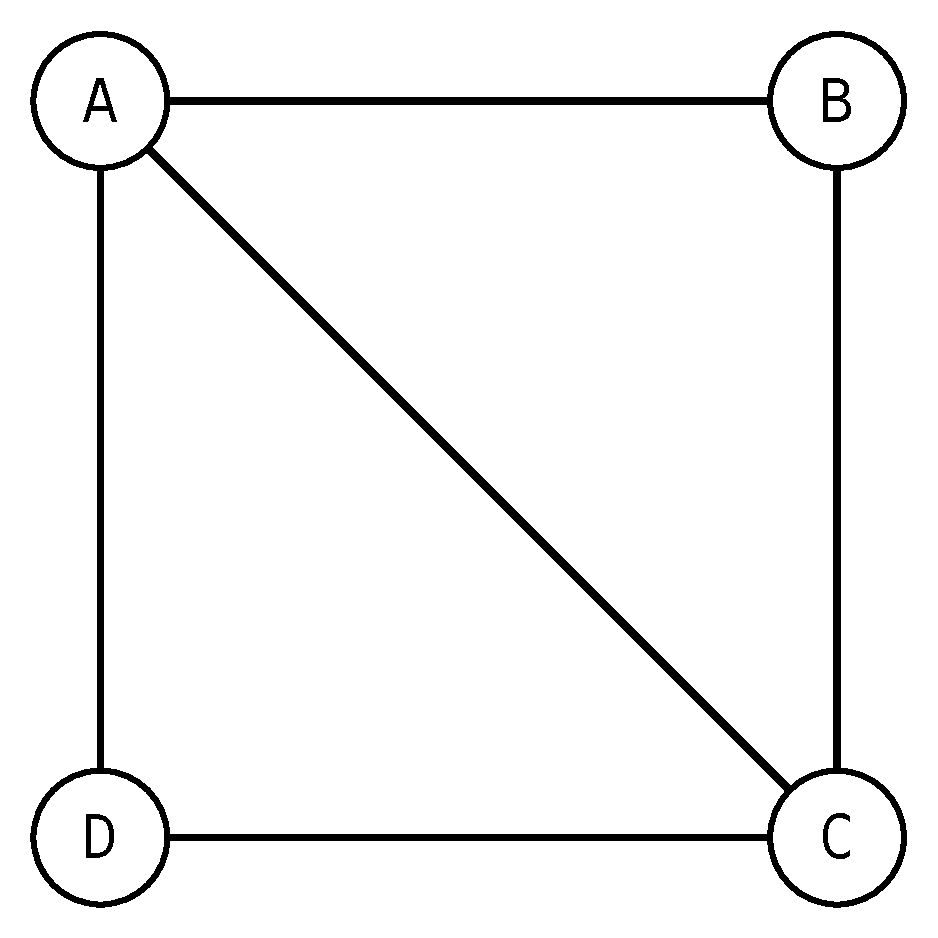
\includegraphics[width=0.32\textwidth]{figures/task-euler-1.pdf}
\end{center}

\smallskip
\textbf{Решение.} Применим критерий Эйлера: связный граф эйлеров (есть эйлеров
цикл) $\Leftrightarrow$ все степени вершин чётны; полуэйлеров (есть эйлеров
путь, но не цикл) $\Leftrightarrow$ ровно две вершины нечётной степени.

Подсчитаем степени:
\[
  \deg A=3\ (B,D,C),\quad \deg B=2\ (A,C),\quad \deg C=3\ (B,D,A),\quad \deg D=2\ (C,A).
\]
Нечётную степень имеют ровно две вершины --- $A$ и $C$. Следовательно, граф
\emph{полуэйлеров}: эйлерова цикла нет, но есть эйлеров путь, причём он обязан
начинаться и заканчиваться в нечётных вершинах $A$ и $C$.

Построим путь (например, алгоритмом Флёри, не выбирая мост, пока есть
альтернатива): 
\[
  A \to B \to C \to D \to A \to C.
\]
Он проходит по всем пяти рёбрам $AB,BC,CD,DA,AC$ ровно по одному разу
(номера на рёбрах --- порядок прохождения):

\begin{center}
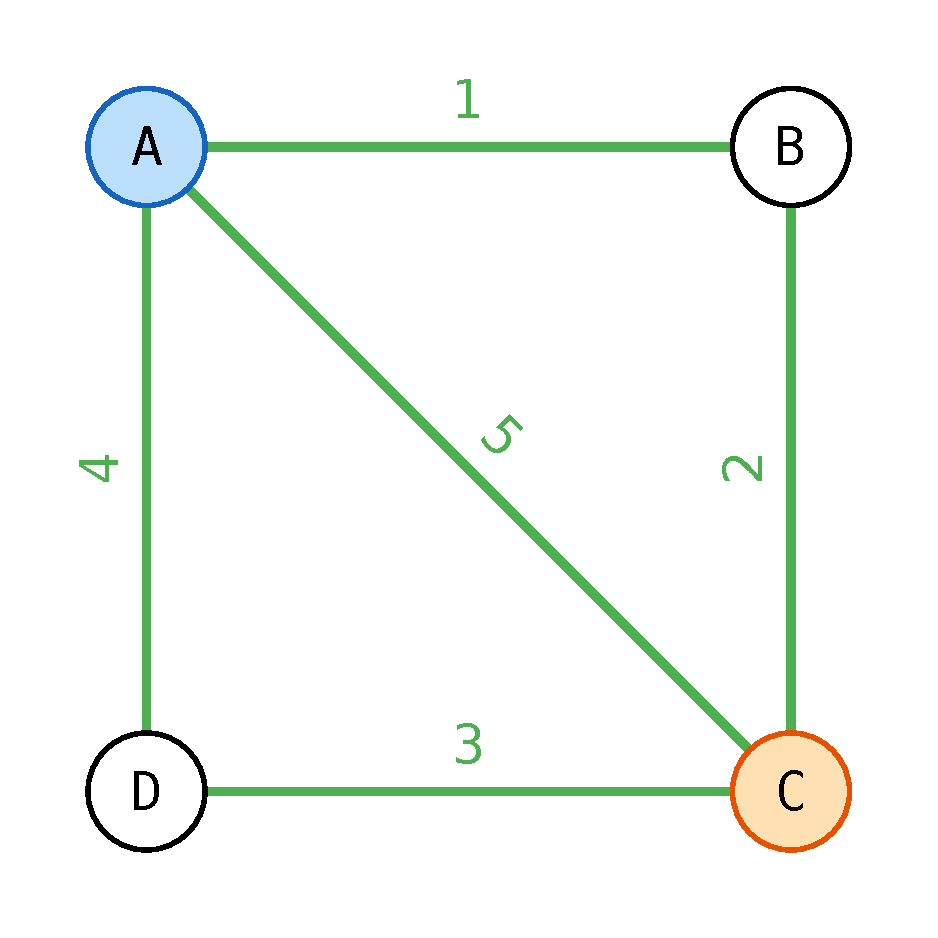
\includegraphics[width=0.32\textwidth]{figures/task-euler-2.pdf}
\end{center}

\textbf{Ответ.} Граф полуэйлеров; эйлеров путь $A\!-\!B\!-\!C\!-\!D\!-\!A\!-\!C$
(из $A$ в $C$). Эйлерова цикла нет, так как есть вершины нечётной степени.
\end{task}

% ============================================================
\begin{task}{Компоненты сильной связности: алгоритм Косарайю}{kosaraju-task}
\textbf{Условие.} Дан ориентированный граф на вершинах $A,B,C,D,E$ с дугами
\[
  A\!\to\!B,\ B\!\to\!C,\ C\!\to\!A,\ B\!\to\!D,\ D\!\to\!E,\ E\!\to\!D.
\]
Найдите компоненты сильной связности алгоритмом Косарайю.

\begin{center}
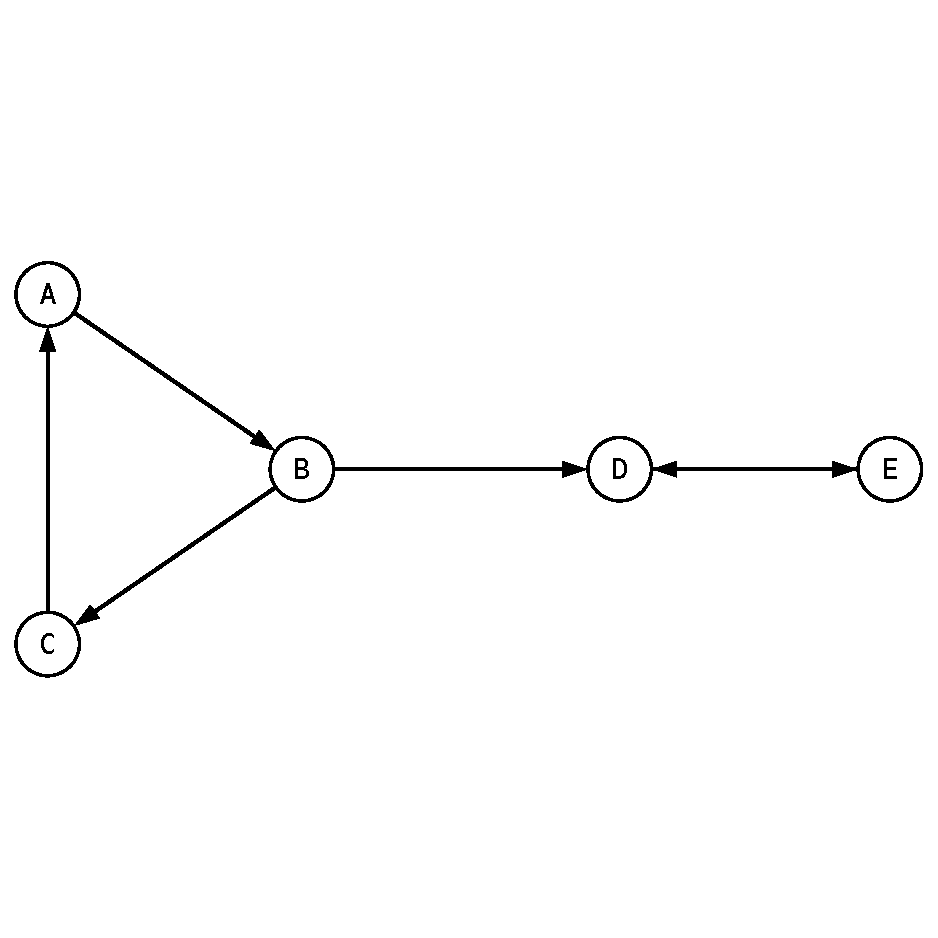
\includegraphics[width=0.45\textwidth]{figures/task-scc-1.pdf}
\end{center}

\smallskip
\textbf{Решение.} Алгоритм Косарайю состоит из трёх шагов: (1)~обход в глубину
исходного графа $G$ с записью времён выхода; (2)~построение транспонированного
графа $G^{T}$ (все дуги развёрнуты); (3)~обход $G^{T}$ в порядке убывания времён
выхода --- каждое дерево обхода даёт одну компоненту.

\textbf{Шаг 1. DFS по $G$ из $A$.} Порядок выхода (по возрастанию):
\[
  C(1),\ E(2),\ D(3),\ B(4),\ A(5).
\]
Порядок убывания времён выхода: $A,\ B,\ D,\ E,\ C$.

\textbf{Шаг 2. Транспонированный граф $G^{T}$:}
\[
  B\!\to\!A,\ C\!\to\!B,\ A\!\to\!C,\ D\!\to\!B,\ E\!\to\!D,\ D\!\to\!E.
\]

\textbf{Шаг 3. DFS по $G^{T}$ в порядке $A,B,D,E,C$.}
\begin{itemize}
  \item Из $A$: $A\!\to\!C\!\to\!B\!\to\!A$ --- собрана компонента $\{A,B,C\}$.
  \item Следующая непосещённая (по порядку) --- $D$: $D\!\to\!E\!\to\!D$ ---
        компонента $\{D,E\}$.
\end{itemize}

\begin{center}
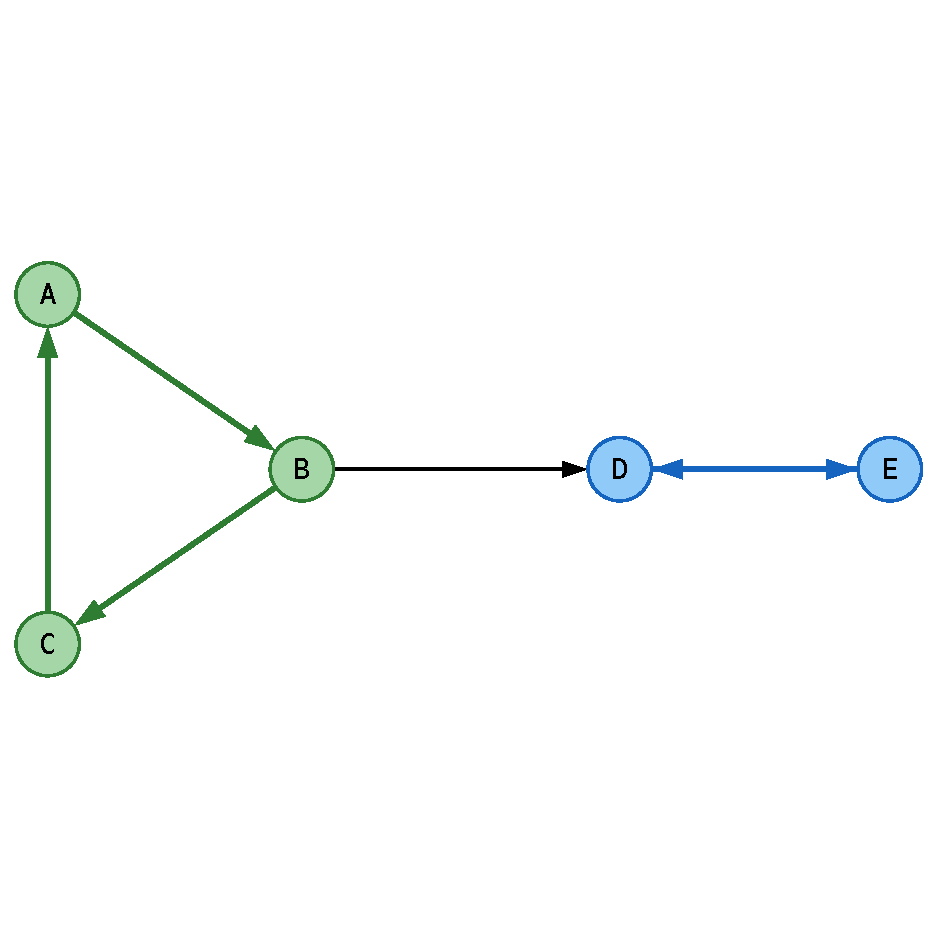
\includegraphics[width=0.45\textwidth]{figures/task-scc-2.pdf}
\end{center}

\textbf{Ответ.} Две компоненты сильной связности: $\{A,B,C\}$ (цикл
$A\!\to\!B\!\to\!C\!\to\!A$) и $\{D,E\}$ (цикл $D\!\leftrightarrows\!E$). Дуга
$B\!\to\!D$ соединяет компоненты в одном направлении, поэтому в одну компоненту
они не объединяются.
\end{task}


\chapter{Лекция 6. Гамильтоновы графы. Графы де Брёйна. Деревья}

% ============================================================
% ГАМИЛЬТОНОВЫ ГРАФЫ (стр. 15, dir2 стр. 3)
% ============================================================

\subsection*{Гамильтоновы графы}

\begin{defn}{Гамильтонов путь}{hamilton-path}
$G(V, E)$.

$G$ содержит \textbf{гамильтонов путь} $\;\Leftrightarrow\;$ $\exists$ путь, проходящий через
$\forall\, v \in V$ ровно 1 раз.

$\Rightarrow\;$ $G$ --- \textbf{полугамильтонов}.
\end{defn}

\begin{defn}{Гамильтонов цикл}{hamilton-cycle}
$G$ содержит \textbf{гамильтонов цикл} $\;\Leftrightarrow\;$ $\exists$ замкнутый простой путь через
$\forall\, v \in V$ ровно 1 раз, кроме $v_{\text{start}} = v_{\text{finish}}$.

$\Rightarrow\;$ $G$ --- \textbf{гамильтонов}.
\end{defn}

\medskip
\noindent\textbf{Примеры:}

% Пример 1: путь 1—2—3—4 — полугамильтонов
% Граф: p15-example-1.graph
\grfig{figures/p15-example-1.pdf}{Полугамильтонов: цепь $1$--$2$--$3$--$4$}
\noindent\textit{Пример 1.} Цепь $1$--$2$--$3$--$4$ сама является гамильтоновым
путём (каждая вершина ровно один раз), но цикла нет --- граф
\textbf{полугамильтонов}.

% Пример 2: цикл 1—2—3—4—1 — гамильтонов (и полугамильтонов)
% Граф: p15-example-2.graph
\grfig{figures/p15-example-2.pdf}{Гамильтонов (и полугамильтонов): цикл $1$--$2$--$3$--$4$--$1$}
\noindent\textit{Пример 2.} Цикл $1$--$2$--$3$--$4$--$1$ --- гамильтонов цикл,
поэтому граф \textbf{гамильтонов} (а значит, и \textbf{полугамильтонов}:
убрав последнее ребро цикла, получаем гамильтонов путь).

% Пример 3: 1—2—3, 2—4 (звезда) — ни гам., ни полугам.
% Граф: p15-example-3.graph
\grfig{figures/p15-example-3.pdf}{Ни гамильтонов, ни полугамильтонов: $1$--$2$--$3$, $2$--$4$}
\noindent\textit{Пример 3.} <<Звезда>> $1$--$2$--$3$ c дополнительным листом
$2$--$4$: любой путь, заходящий во все три листа $1, 3, 4$, обязан
проходить через центр $2$ минимум дважды --- граф \textbf{ни гамильтонов,
ни полугамильтонов}.

\medskip
\textbf{Замечание.} Теоремы ниже дают только \emph{достаточные} условия
гамильтоновости: если условие выполнено --- граф точно гамильтонов, но если
условие \emph{не} выполнено, это ещё не значит, что граф не гамильтонов
(например, цикл $C_5$ гамильтонов, хотя все степени равны $2 < 5/2$).

\medskip
Условия гамильтоновости ($G(V,E)$ --- неориент., связный):

\begin{statement}{Теорема Оре}{ore}
$|V| = n \ge 3$. Если $\forall\, u, v \in V$ т.\,ч. $\nexists\, e = uv$
\textup{($u, v$ --- несмежные)}:
$\deg(u) + \deg(v) \geq n$,
то $G$ --- гамильтонов.
\end{statement}

\begin{proof}
От противного. Пусть условие выполнено, но гамильтонова цикла нет. Будем
добавлять в $G$ рёбра, пока это возможно без появления гамильтонова цикла
(условие Оре при добавлении рёбер тем более сохраняется); получим
\emph{максимальный} контрпример $G'$: гамильтонова цикла нет, но
добавление любого ребра его создаёт.

В $G'$ есть несмежные вершины $u, v$ (иначе $G' = K_n$ --- гамильтонов).
Добавление ребра $uv$ создаёт гамильтонов цикл, значит уже в $G'$ есть
гамильтонов \emph{путь} $u = v_1, v_2, \ldots, v_n = v$.

Рассмотрим множества индексов
$S = \{\, i \mid u \sim v_{i+1} \,\}$ и $T = \{\, i \mid v \sim v_i \,\}$;
$|S| = \deg(u)$, $|T| = \deg(v)$, причём $S, T \subseteq \{1, \dots, n-1\}$.
Так как $|S| + |T| = \deg(u) + \deg(v) \ge n > n - 1$, по принципу Дирихле
$\exists\, i \in S \cap T$: одновременно $u \sim v_{i+1}$ и $v \sim v_i$.
Тогда
\[
  u = v_1, v_2, \ldots, v_i,\; v_n = v,\; v_{n-1}, \ldots, v_{i+1},\; v_1
\]
--- гамильтонов цикл (идём по пути до $v_i$, прыгаем по ребру $v_i v_n$
в конец, возвращаемся по пути назад до $v_{i+1}$ и замыкаемся ребром
$v_{i+1} u$). Противоречие с тем, что в $G'$ цикла нет.
\end{proof}

\begin{statement}{Теорема Дирака}{dirac}
$|V| = n \ge 3$. Если $\forall\, u \in V$: $\deg(u) \geq \dfrac{n}{2}$,
то $G$ --- гамильтонов.
\end{statement}

\begin{proof}
Частный случай теоремы Оре: для любых несмежных $u, v$ имеем
$\deg(u) + \deg(v) \ge \frac{n}{2} + \frac{n}{2} = n$.
\end{proof}

\begin{defn}{Турнир}{tournament}
\textbf{Турнир} --- ориентированный граф, в котором каждая пара
различных вершин соединена \emph{ровно одной} дугой (в одном из двух
направлений). Иначе говоря, турнир --- это полный граф $K_n$, каждому
ребру которого приписана ориентация.
\end{defn}

\grfig[0.42]{figures/p15-tournament-1.pdf}{Турнир на 4 вершинах: гамильтонов путь $1 \to 2 \to 3 \to 4$}

\textbf{Примеры.} 1) Результаты кругового спортивного турнира без
ничьих: вершины --- участники, дуга $u \to v$ означает <<$u$ выиграл у
$v$>> (отсюда и название). На рисунке: $1$ победил всех, $4$ проиграл
всем, между $2$ и $3$ --- победа $2$. 2) Транзитивный турнир: вершины
$1, \ldots, n$, все дуги от меньшего номера к большему --- это в
точности строгий линейный порядок из лекции 3.

\begin{statement}{Теорема Редеи (о турнирах)}{redei}
В любом турнире существует гамильтонов путь.
\end{statement}

\begin{proof}
Индукция по числу вершин $n$. База $n = 1$ тривиальна. Переход: удалим
из турнира вершину $v$; на оставшихся $n - 1$ вершинах по предположению
индукции есть гамильтонов путь $u_1 \to u_2 \to \ldots \to u_{n-1}$.
Вставим $v$:
\begin{itemize}
  \item если $v \to u_1$ --- ставим $v$ в начало;
  \item иначе $u_1 \to v$; пусть $i$ --- наибольший индекс с
        $u_i \to v$. Если $i = n - 1$, ставим $v$ в конец. Если же
        $i < n - 1$, то по максимальности $v \to u_{i+1}$, и $v$
        вставляется между $u_i$ и $u_{i+1}$:
        $u_1 \to \ldots \to u_i \to v \to u_{i+1} \to \ldots \to u_{n-1}$.
\end{itemize}
В каждом случае получили гамильтонов путь на всех $n$ вершинах
(заметим: гамильтонов \emph{цикл} в турнире существовать не обязан ---
в транзитивном турнире из последней вершины дуги не выходят).
\end{proof}

% ============================================================
% Построение гамильтонова пути (в условиях т. Дирака)
% (стр. 15–16, dir2 стр. 3–4)
% ============================================================

\begin{algo}{Построение гамильтонова пути в условиях теоремы Дирака}{hamilton-dirac}

\textbf{Инициализация:} $v_1, v_2, \ldots, v_n$ --- произвольный порядок
\emph{всех} вершин графа.

\textbf{Шаг (поворот):} пока в последовательности есть несмежная соседняя
пара $(v_i, v_{i+1})$, ищем индекс $j > i + 1$, для которого
\emph{оба} ребра существуют:
\[
  \exists\, e_1 = v_i v_j \quad\text{и}\quad \exists\, e_2 = v_{i+1} v_{j+1};
\]
(условие Дирака гарантирует, что такой $j$ найдётся). Переворачиваем
отрезок $v_{i+1} \ldots v_j$:
\[
  v_1 \ldots v_i \;\bigl|\; \underbrace{v_j \, v_{j-1} \ldots v_{i+1}}_{\text{перевёрнут}} \;\bigl|\; v_{j+1} \ldots v_n.
\]
На стыках теперь стоят пары $(v_i, v_j)$ и $(v_{i+1}, v_{j+1})$ ---
обе смежные, а внутри перевёрнутого отрезка смежность пар не изменилась.
Число несмежных пар строго уменьшилось; повторяем, пока их не останется
--- получился гамильтонов путь.

\medskip
\noindent\textbf{Пример.} Возьмём граф с рёбрами
$A$--$C$, $C$--$E$, $E$--$F$, $F$--$D$, $D$--$B$, $B$--$A$, $A$--$D$,
$C$--$F$, $B$--$E$ (к графу с рис. выше по тексту добавлено ребро
$B$--$E$, чтобы выполнялось условие Дирака: теперь все степени равны
$3 = \frac{6}{2} = \frac{n}{2}$).

\grfig[0.5]{figures/p15-example-4b.pdf}{Алг. Дирака: граф $A,\dots,F$, все степени $= 3$}

Начальный порядок: $E, A, B, D, F, C$ --- т.\,е.
$v_1 = E,\; v_2 = A,\; v_3 = B,\; v_4 = D,\; v_5 = F,\; v_6 = C$.
Порядок \emph{произвольный} (алгоритм стартует с любого); этот выбран
для компактности примера --- в нём всего одна несмежная соседняя пара.
Проверяем пары: $(E, A)$ --- \emph{несмежная} (ребра $E$--$A$ нет);
остальные пары $(A,B), (B,D), (D,F), (F,C)$ --- смежные.

Чиним пару $(v_i, v_{i+1}) = (v_1, v_2) = (E, A)$. По описанию шага ищем
индекс $j > i + 1 = 2$, для которого существуют \emph{оба} ребра
$v_i v_j$ и $v_{i+1} v_{j+1}$, т.\,е. $E \sim v_j$ и $A \sim v_{j+1}$
--- перебираем кандидатов $j = 3, 4, 5$ по порядку:
\begin{itemize}
  \item $j = 3$: $v_3 = B$, $v_4 = D$. Проверяем: $E \sim B$? --- да
        (ребро $B$--$E$); $A \sim D$? --- да (ребро $A$--$D$).
        \textbf{Оба условия выполнены} --- берём $j = 3$ (дальше можно
        не перебирать; для сравнения: $j = 4$ не подошёл бы --- уже
        первое условие $E \sim v_4 = D$ не выполнено, ребра $E$--$D$
        в графе нет).
\end{itemize}
Переворачиваем отрезок $v_{i+1} \ldots v_j = v_2 \ldots v_3 = (A, B)$:
\[
  E,\; \underline{A,\; B},\; D,\; F,\; C
  \quad\longrightarrow\quad
  E,\; \underline{B,\; A},\; D,\; F,\; C.
\]
На стыках перевёрнутого отрезка встали проверенные рёбра: слева ---
$v_1 v_3 = E$--$B$, справа --- $v_2 v_4 = A$--$D$.
Все соседние пары теперь смежные: $E$--$B$, $B$--$A$, $A$--$D$, $D$--$F$,
$F$--$C$ --- это \textbf{гамильтонов путь}. Более того, концы $E$ и $C$
тоже смежны ($C$--$E$ --- ребро), так что путь замыкается в
\textbf{гамильтонов цикл} $E, B, A, D, F, C, E$.

\medskip
\noindent\textbf{Работа алгоритма по шагам} (синие рёбра --- смежные
соседние пары, красное --- несмежная пара, зелёные --- рёбра поворота
и итоговый путь):

\begin{center}\begin{tabular}{cc}
\shortstack{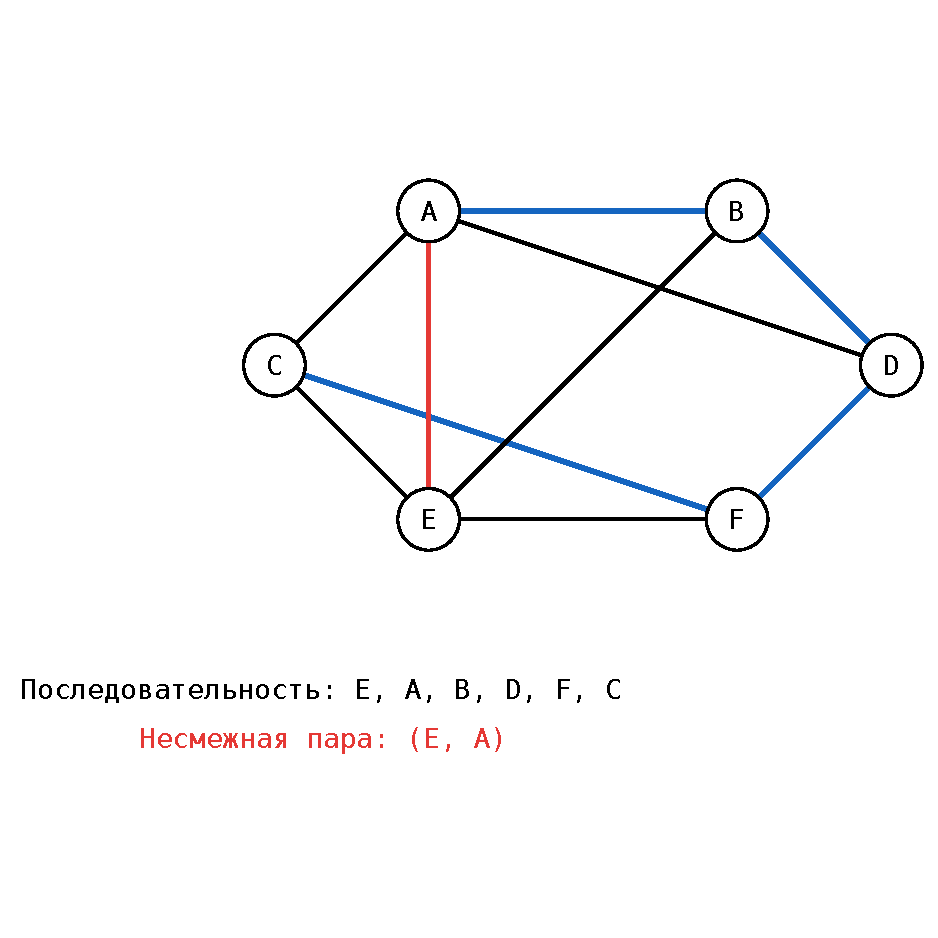
\includegraphics[width=0.46\textwidth]{python/lec06/hamilton/hamilton-0.pdf}\\[2pt]{\scriptsize Шаг 0. Порядок $E,A,B,D,F,C$; пара $(E,A)$ несмежная}} &
\shortstack{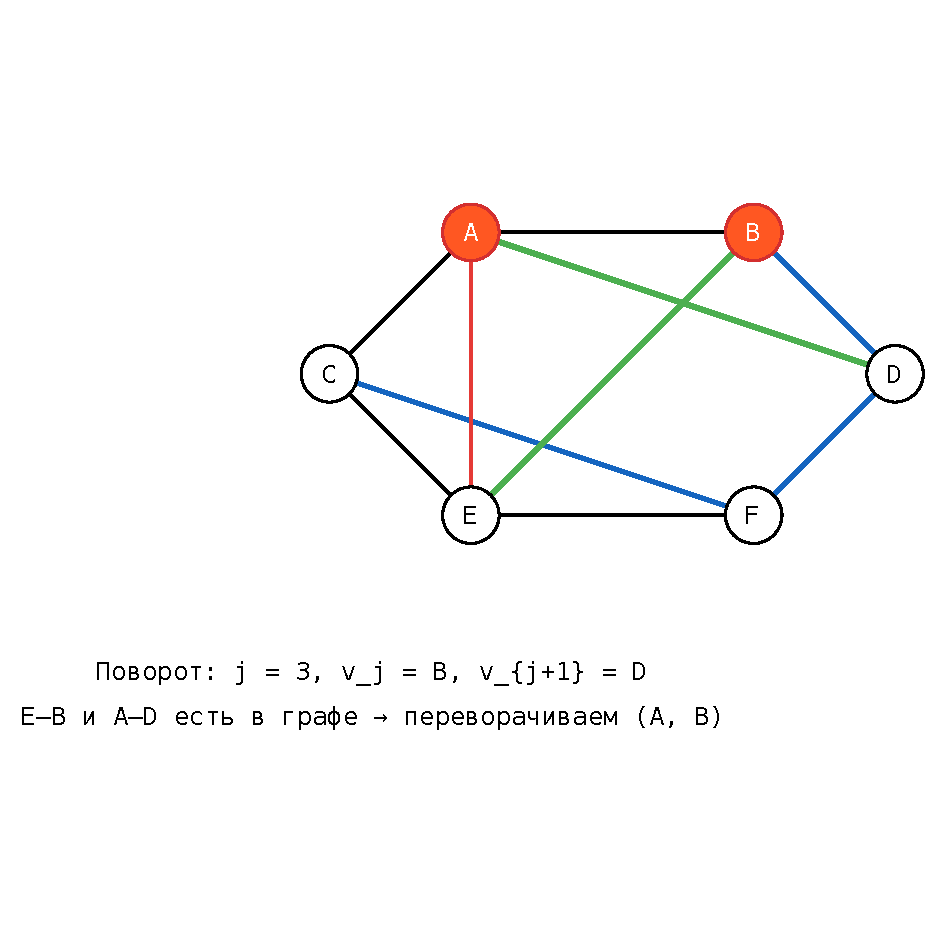
\includegraphics[width=0.46\textwidth]{python/lec06/hamilton/hamilton-1.pdf}\\[2pt]{\scriptsize Шаг 1. Поворот: $j=3$, рёбра $E$--$B$ и $A$--$D$ есть}} \\
\end{tabular}\end{center}
\begin{center}\begin{tabular}{cc}
\shortstack{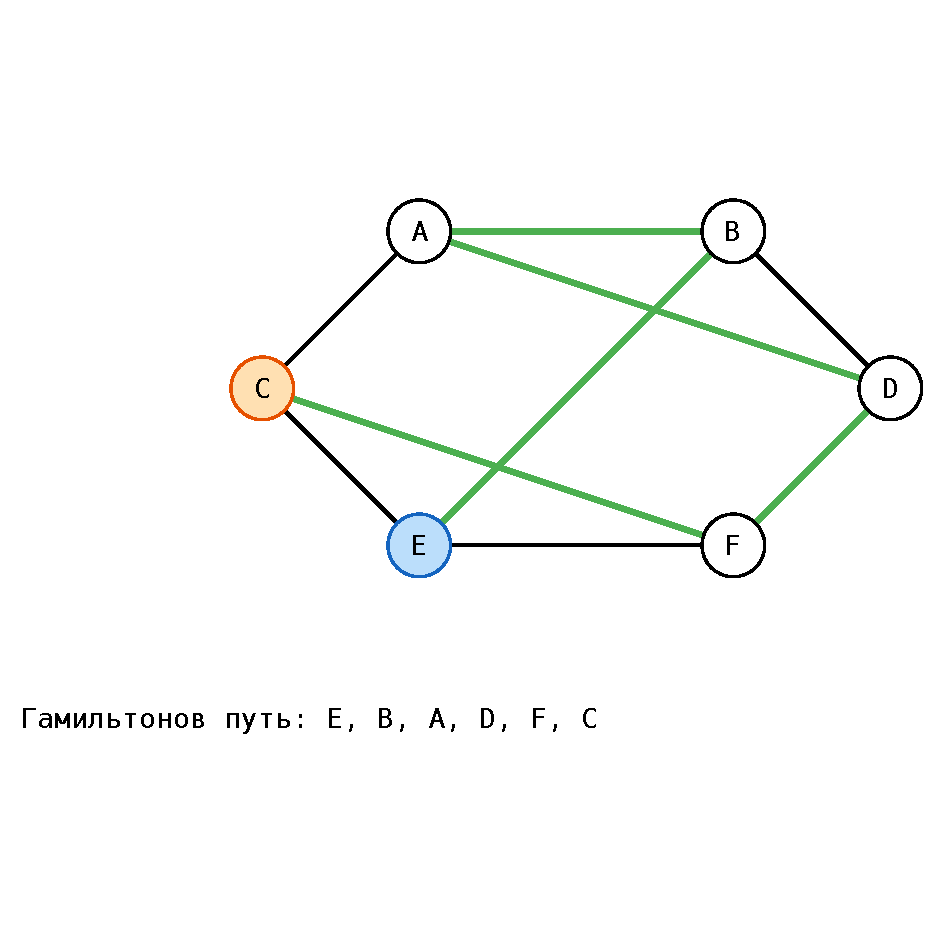
\includegraphics[width=0.46\textwidth]{python/lec06/hamilton/hamilton-2.pdf}\\[2pt]{\scriptsize Шаг 2. Отрезок $(A,B)$ перевёрнут: гамильтонов путь}} &
\shortstack{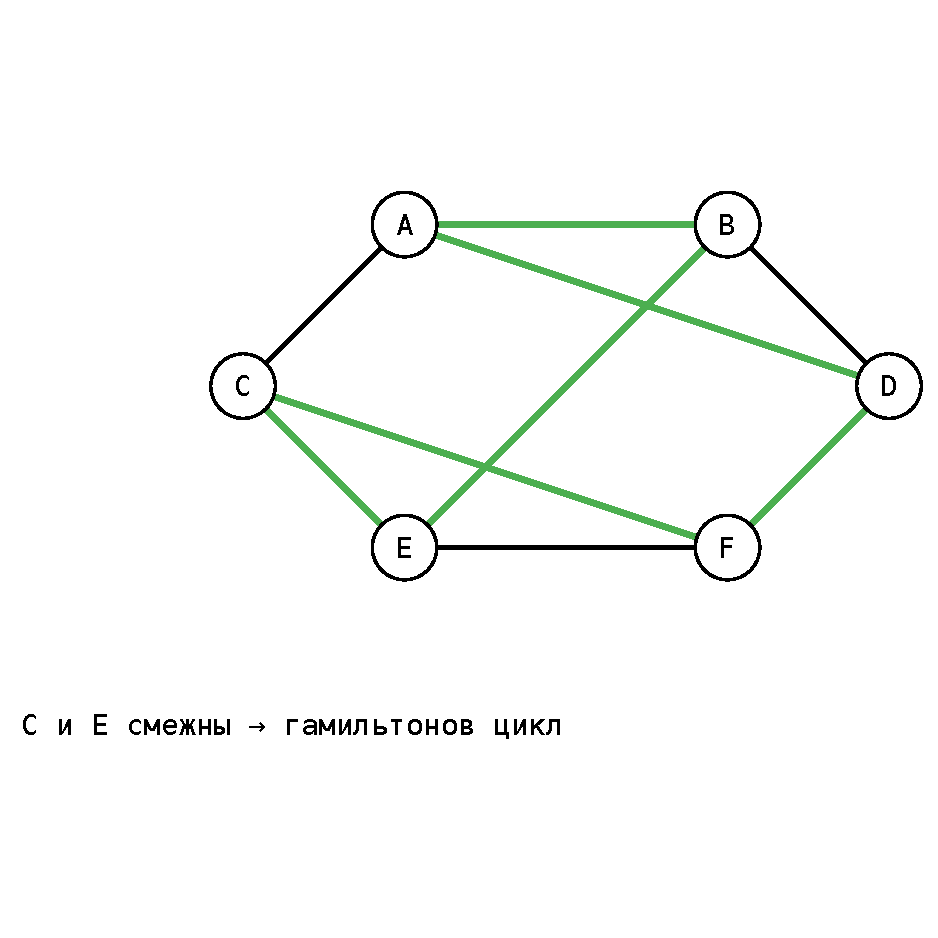
\includegraphics[width=0.46\textwidth]{python/lec06/hamilton/hamilton-3.pdf}\\[2pt]{\scriptsize Шаг 3. $C \sim E$: замыкаем в гамильтонов цикл}} \\
\end{tabular}\end{center}
\end{algo}

% ============================================================
% ГРАФЫ ДЕ БРЁЙНА (стр. 16, dir2 стр. 4)
% ============================================================

\subsection*{Графы де Брёйна}

\begin{defn}{Граф де Брёйна}{de-bruijn}
$\Sigma = \{a_0, \ldots, a_{k-1}\}$ --- алфавит.

$\Sigma^m = \{a_{i_1} \ldots a_{i_m} \mid a_{i_j} \in \Sigma\}$ --- слова длины $m$.

$\Sigma^m = V$ \quad (вершины --- слова длины $m$).

$E = \Sigma^{m+1}$ \quad (рёбра --- слова длины $m+1$).

Ребро $a_{i_1} a_{i_2} \ldots a_{i_m} a_{i_{m+1}}$ соединяет вершину
$(a_{i_1} \ldots a_{i_m})$ с вершиной $(a_{i_2} \ldots a_{i_{m+1}})$:
суффикс первой вершины совпадает с префиксом второй;
$a_{i_1}$ и $a_{i_{m+1}}$ --- любые.

$B(\Sigma, m)$ --- \textbf{граф де Брёйна}.
\end{defn}

\medskip
\noindent\textbf{Пример.}
$\Sigma = \{0, 1\}$, $m = 2$.

% Граф: p16-example-2.graph
\grfig{figures/p16-example-2.pdf}{Граф де Брёйна B(\{0,1\}, 2)}
% Вершины: 00, 01, 10, 11
% Рёбра:
%   00→01 (001), 01→11 (011), 11→10 (110), 10→00 (100)
%   01→10 (010), 10→01 (101)
%   00→00 (000, петля), 11→11 (111, петля)

$\Sigma^2 = \{00, 01, 10, 11\}$ --- вершины.

$B(\{0,1\}, 2)$: рёбра --- все слова длины 3 ($000, 001, 010, 011, 100, 101, 110, 111$).

\medskip
\begin{statement}{Графы де Брёйна всегда эйлеровы}{de-bruijn-euler}
$\forall\, \Sigma$ ($|\Sigma| = k$), $\forall\, m$: граф $B(\Sigma, m)$ ---
эйлеров.
\end{statement}

\begin{proof}
Проверим критерий эйлеровости для ориентированного графа.

\textbf{Полустепени равны.} Из вершины $w = a_{i_1} \ldots a_{i_m}$ выходит
ровно $k$ дуг --- слова $w \cdot a$ для каждой буквы $a \in \Sigma$
(ведут в вершины $a_{i_2} \ldots a_{i_m} a$). Входит в $w$ тоже ровно $k$
дуг --- слова $a \cdot w$ для каждой $a \in \Sigma$. Значит,
$\delta^-(v) = \delta^+(v) = k$ для всех вершин.

\textbf{Связность.} Из любой вершины $u = a_{i_1} \ldots a_{i_m}$ можно
дойти до любой вершины $v = b_{j_1} \ldots b_{j_m}$: последовательно
<<вдвигаем>> буквы слова $v$ справа --- за $m$ шагов
$u \to a_{i_2} \ldots a_{i_m} b_{j_1} \to \ldots \to b_{j_1} \ldots b_{j_m} = v$.
Граф даже сильно связен.

Оба условия критерия выполнены --- эйлеров цикл существует. (Именно он
даёт \emph{последовательность де Брёйна} --- кратчайшую циклическую
строку, содержащую все слова длины $m + 1$.)
\end{proof}

% ============================================================
% ДЕРЕВЬЯ (стр. 16–17, dir2 стр. 4–5)
% ============================================================

\subsection*{Деревья}

\begin{defn}{Дерево}{tree}
Ациклический, связный граф.
\end{defn}

Что знаем:
\begin{enumerate}
  \item $G$ --- дерево $\;\Rightarrow\;$ $|E| = |V| - 1$.
  \item $G$ --- связный, $|E| = |V| - 1$ $\;\Rightarrow\;$ $G$ --- дерево.
  \item $G$ --- дерево $\;\Rightarrow\;$ $\forall\, u, v \in V$: $\exists!\;$ цепь.
  \item Если $|V| \geq 4$ $\;\Rightarrow\;$ дерево, $|V|!$, $|E|!$ --- не единственно!
\end{enumerate}

\medskip
\noindent\textbf{Помеченные / непомеченные деревья.}

Помеченные (3 вершины):
$A$--$B$--$C$,\quad $A$--$C$--$B$,\quad $B$--$A$--$C$.

Непомеченные (3 вершины): $\circ$--$\circ$--$\circ$ \quad (единственное).

% ============================================================
% КОД ПРЮФЕРА (стр. 17, dir2 стр. 5)
% ============================================================

\subsection*{Код Прюфера}

Как компактно закодировать помеченное дерево: \textbf{код Прюфера}.

$G(V, E)$ --- дерево, $|V| = n$.

$|\operatorname{Pruf}(G)| = n - 2$.

\begin{algo}{Код Прюфера (прямая задача)}{prufer-encode}
\textbf{Дано:} $G(V, E)$ --- дерево, $|V| = n$, порядок лексикографический.

\textbf{Выход:} $\operatorname{Pruf}(G) = \{v_{i_1}, \ldots, v_{i_{n-2}}\}$.

\textbf{Шаг (step):} удаление лексикографически минимального листа;
в код записывается его родитель (единственный сосед). Повторяем,
пока не останется $2$ вершины: код имеет длину $n - 2$.

% Граф: p17-pruffer-example-1.graph
\grfig[0.55]{figures/p17-pruffer-example-1.pdf}{Код Прюфера: дерево 11 вершин}
% Вершины: A, B, C, D, E, F, H, J, I, K, L (11 вершин)
% Рёбра: A—B, B—C, C—D, D—E, E—F, D—H, H—J, D—I, B—K, C—L

\medskip
\noindent\textbf{Пример.}
Дерево (11 вершин): $A$--$B$, $B$--$C$, $C$--$D$, $D$--$E$, $E$--$F$,
$D$--$H$, $H$--$J$, $D$--$I$, $B$--$K$, $C$--$L$.
Порядок: $A, B, C, D, E, F, H, I, J, K, L$.

\medskip
По шагам (лист $\to$ в код пишем его соседа):
\begin{enumerate}
  \item листья $\{A, F, I, J, K, L\}$; минимальный $A$, сосед $B$ $\to$ код $(B)$;
  \item минимальный лист $F$, сосед $E$ $\to$ код $(B, E)$;
  \item $E$ стала листом; минимальный лист $E$, сосед $D$ $\to$ $(B, E, D)$;
  \item минимальный лист $I$, сосед $D$ $\to$ $(B, E, D, D)$;
  \item минимальный лист $J$, сосед $H$ $\to$ $(B, E, D, D, H)$;
  \item $H$ стала листом; сосед $D$ $\to$ $(B, E, D, D, H, D)$;
  \item $D$ стала листом; сосед $C$ $\to$ $(B, E, D, D, H, D, C)$;
  \item минимальный лист $K$, сосед $B$ $\to$ $(B, E, D, D, H, D, C, B)$;
  \item $B$ стала листом; сосед $C$ $\to$ $(B, E, D, D, H, D, C, B, C)$;
        остались две вершины $C$ и $L$ --- стоп.
\end{enumerate}

\[
  \operatorname{Pruf}(G) = (B,\; E,\; D,\; D,\; H,\; D,\; C,\; B,\; C),
  \qquad |\operatorname{Pruf}(G)| = 11 - 2 = 9.
\]

\medskip
\noindent\textbf{Работа алгоритма по шагам.} На каждом шаге удаляется
лист с минимальной меткой (оранжевый), в код дописывается его сосед
(синий); удалённые вершины и рёбра показаны серым.

\begin{center}\begin{tabular}{ccc}
\shortstack{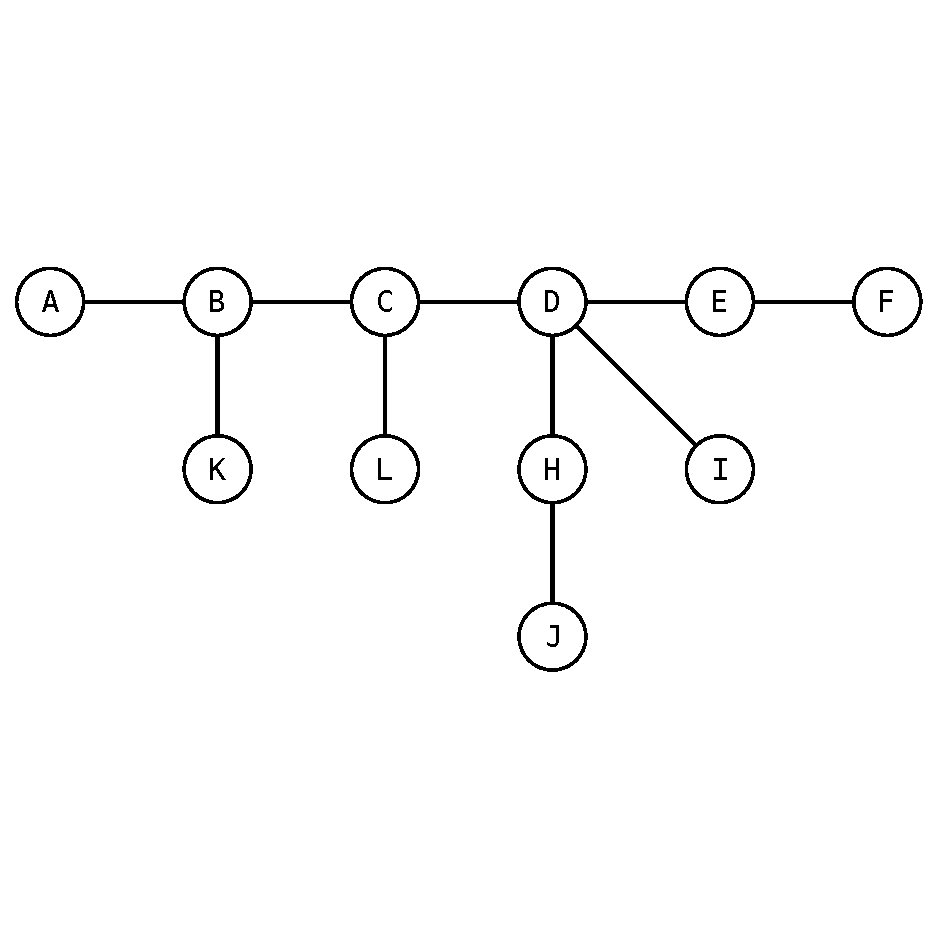
\includegraphics[width=0.28\textwidth]{python/lec06/pruefer/pruefer-0.pdf}\\[2pt]{\scriptsize Шаг 0. Исходное дерево}} &
\shortstack{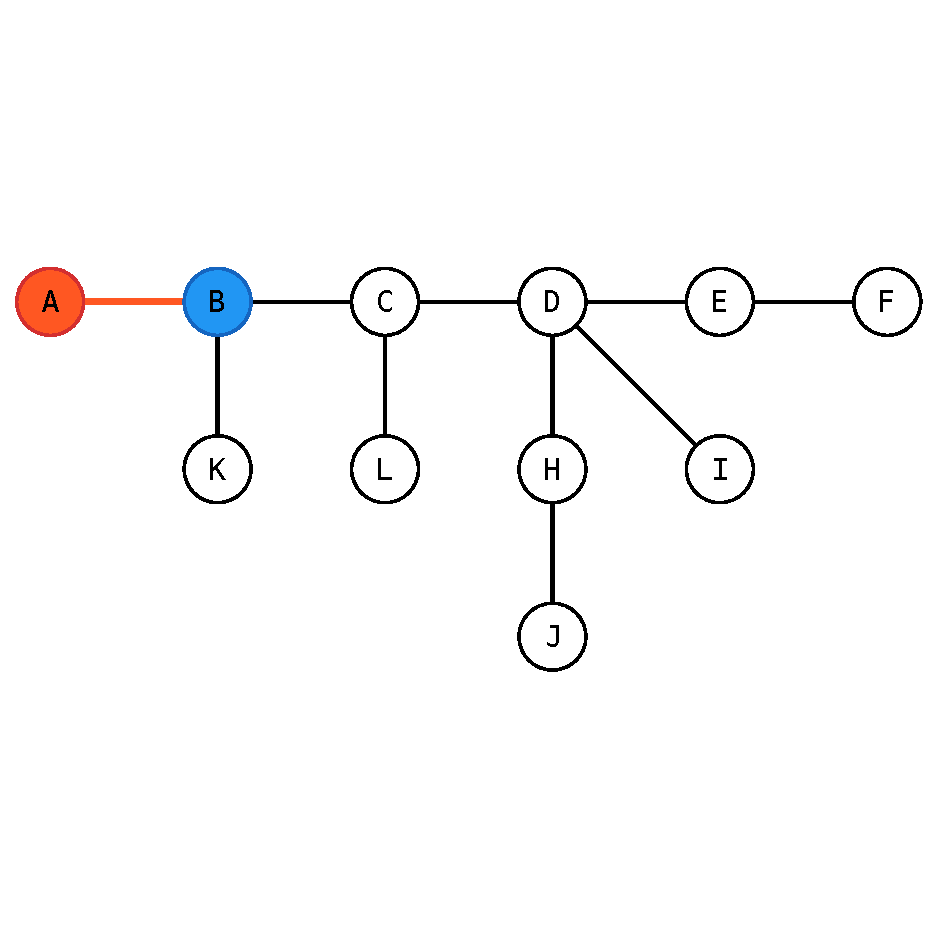
\includegraphics[width=0.28\textwidth]{python/lec06/pruefer/pruefer-1.pdf}\\[2pt]{\scriptsize Шаг 1. $A \to$ код: $B$}} &
\shortstack{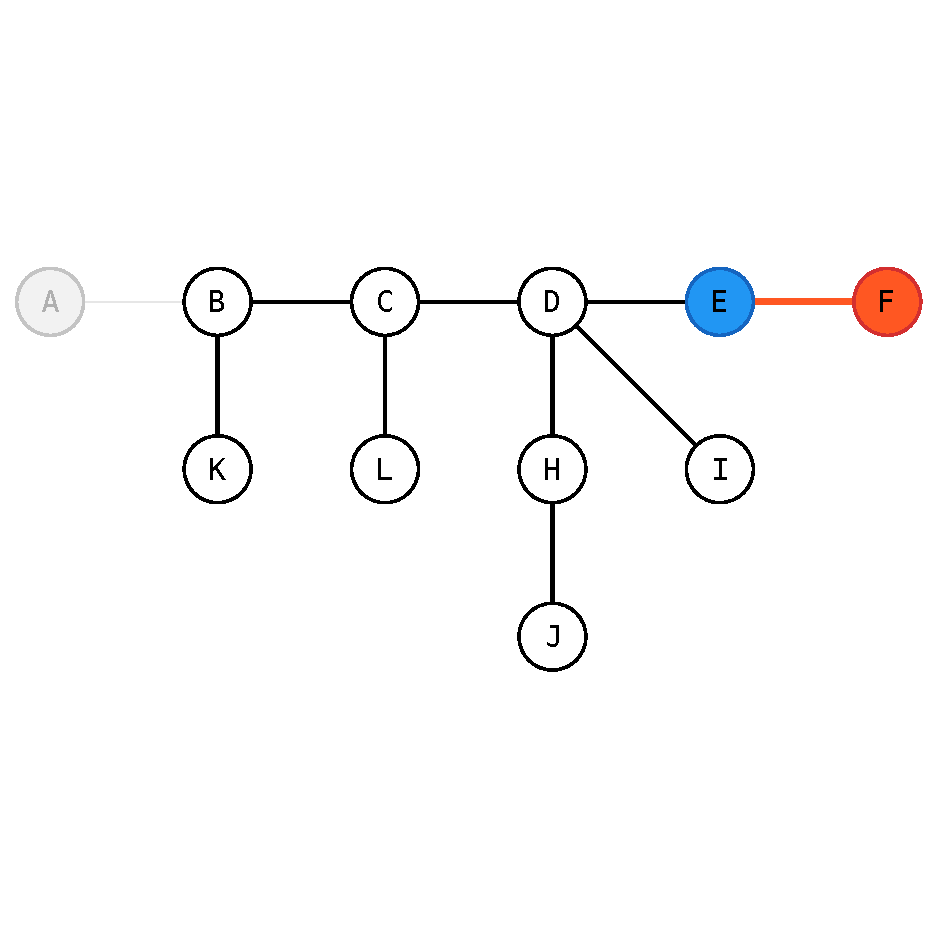
\includegraphics[width=0.28\textwidth]{python/lec06/pruefer/pruefer-2.pdf}\\[2pt]{\scriptsize Шаг 2. $F \to$ код: $E$}} \\
\end{tabular}\end{center}
\begin{center}\begin{tabular}{ccc}
\shortstack{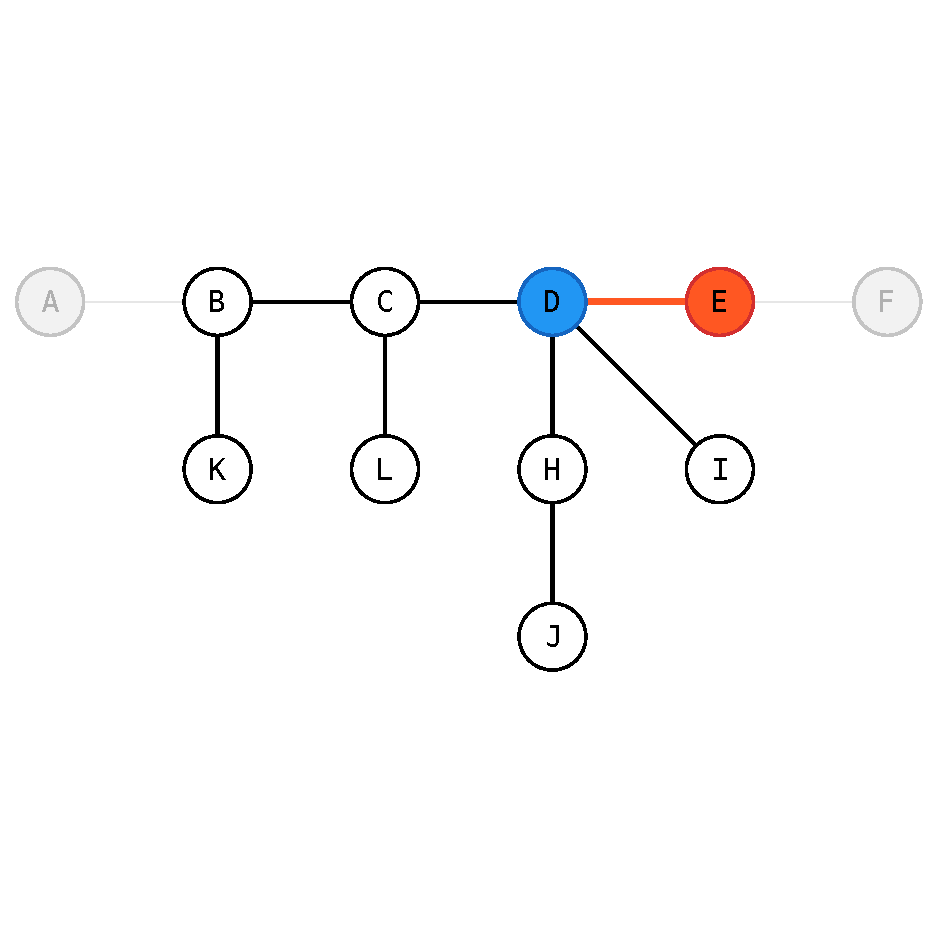
\includegraphics[width=0.28\textwidth]{python/lec06/pruefer/pruefer-3.pdf}\\[2pt]{\scriptsize Шаг 3. $E \to$ код: $D$}} &
\shortstack{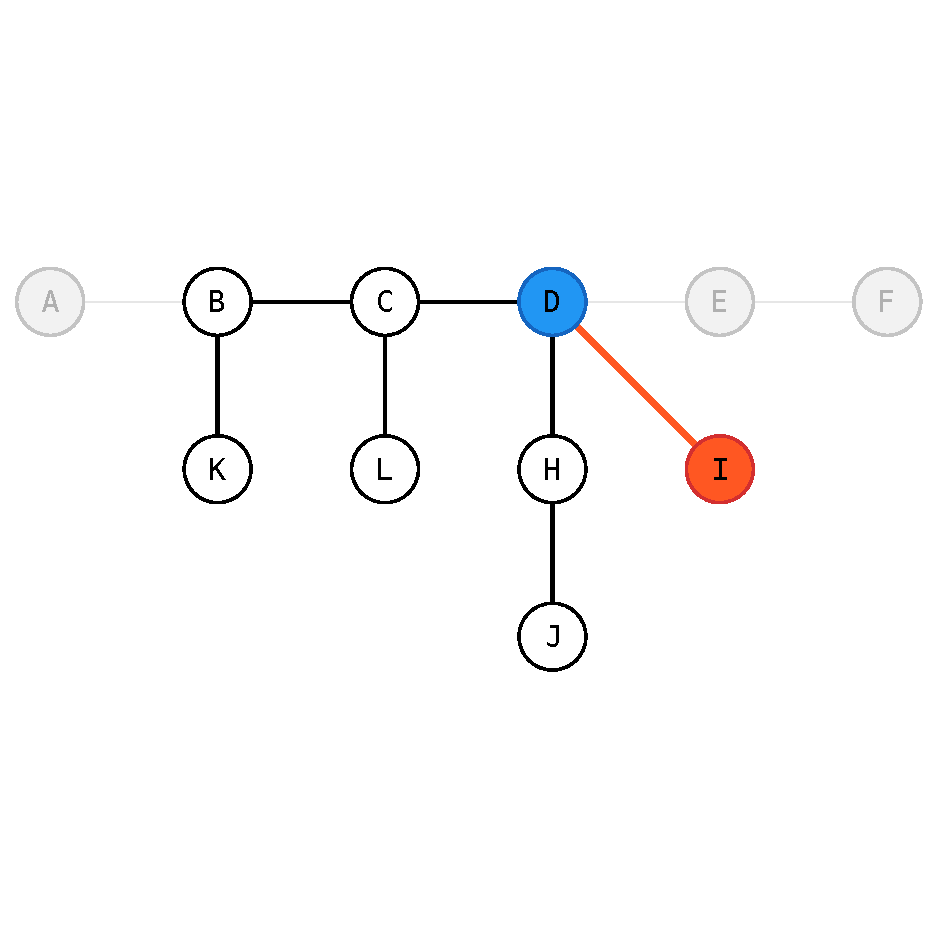
\includegraphics[width=0.28\textwidth]{python/lec06/pruefer/pruefer-4.pdf}\\[2pt]{\scriptsize Шаг 4. $I \to$ код: $D$}} &
\shortstack{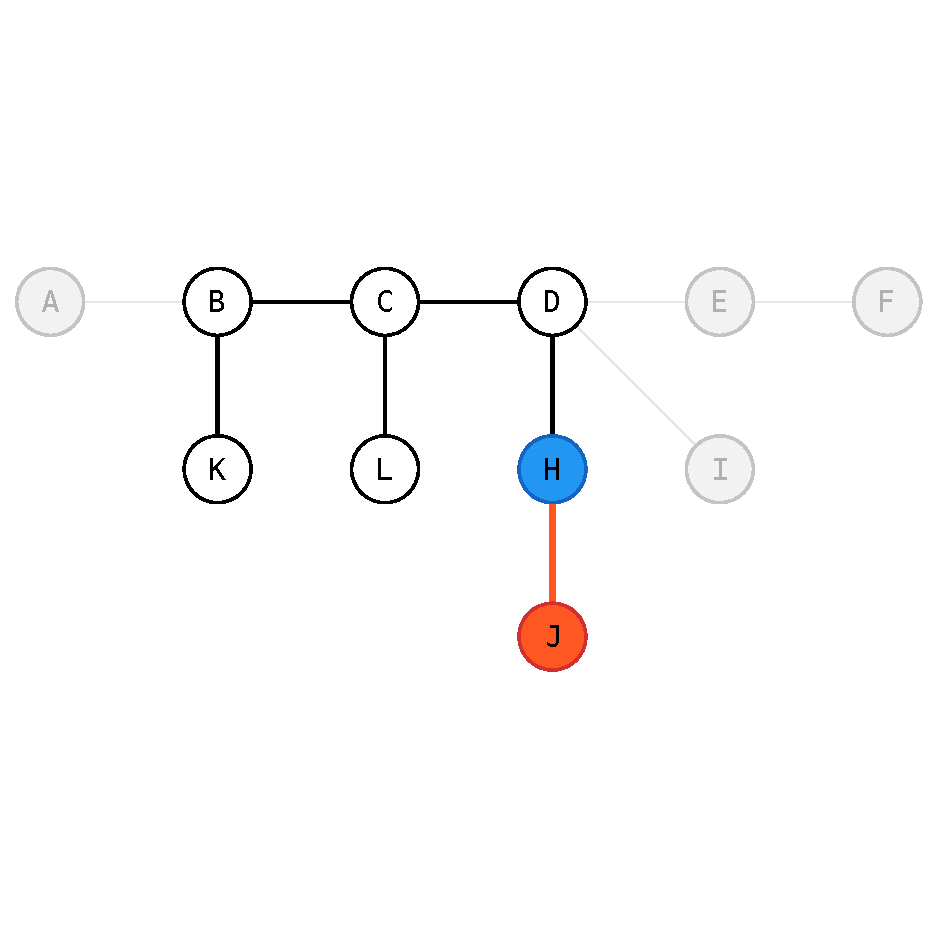
\includegraphics[width=0.28\textwidth]{python/lec06/pruefer/pruefer-5.pdf}\\[2pt]{\scriptsize Шаг 5. $J \to$ код: $H$}} \\
\end{tabular}\end{center}
\begin{center}\begin{tabular}{ccc}
\shortstack{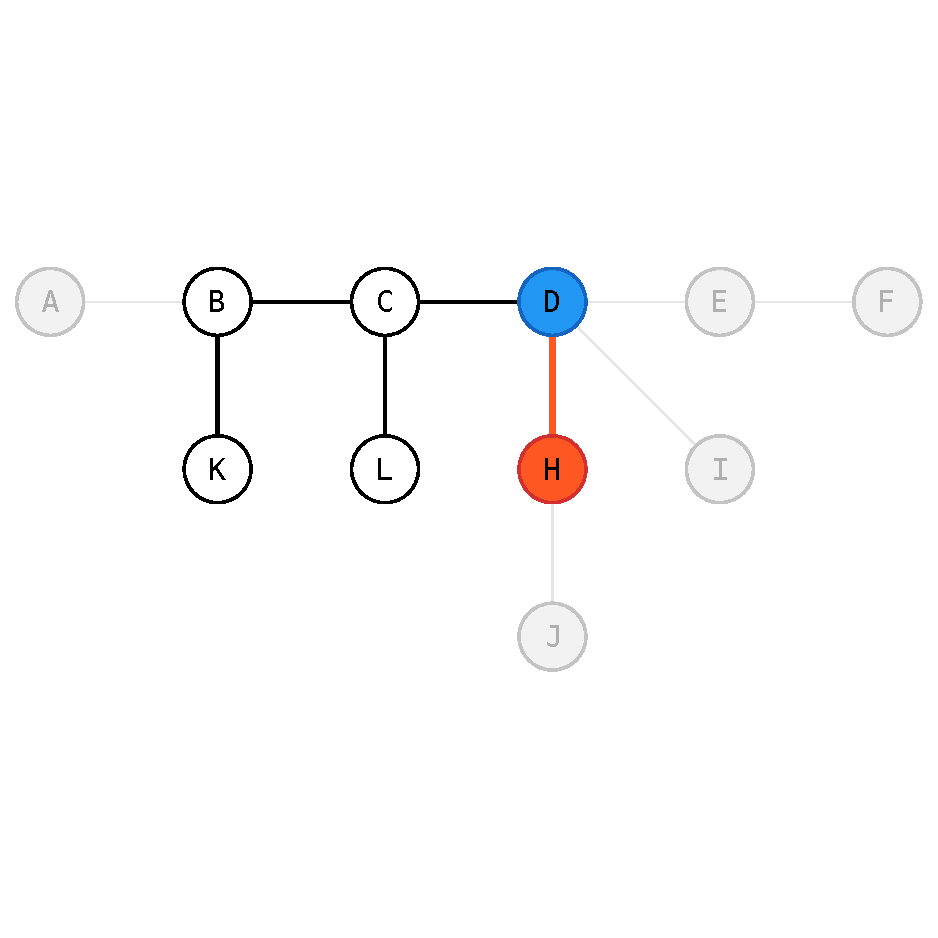
\includegraphics[width=0.28\textwidth]{python/lec06/pruefer/pruefer-6.pdf}\\[2pt]{\scriptsize Шаг 6. $H \to$ код: $D$}} &
\shortstack{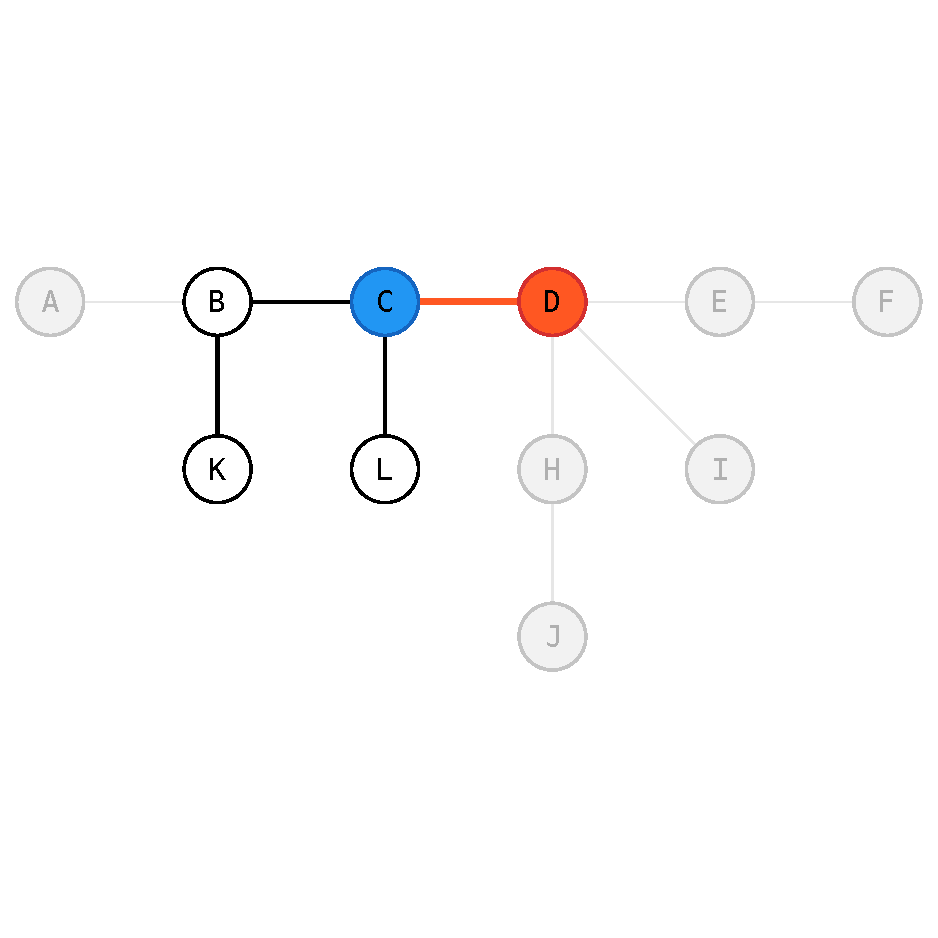
\includegraphics[width=0.28\textwidth]{python/lec06/pruefer/pruefer-7.pdf}\\[2pt]{\scriptsize Шаг 7. $D \to$ код: $C$}} &
\shortstack{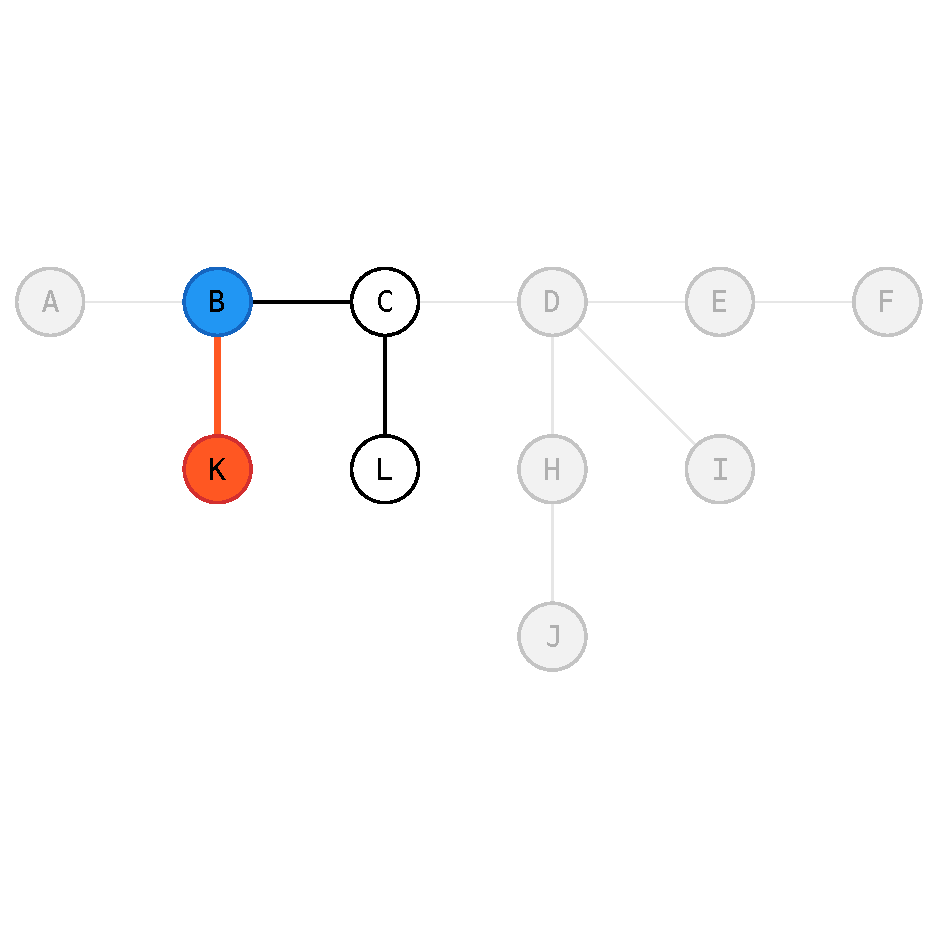
\includegraphics[width=0.28\textwidth]{python/lec06/pruefer/pruefer-8.pdf}\\[2pt]{\scriptsize Шаг 8. $K \to$ код: $B$}} \\
\end{tabular}\end{center}
\begin{center}\begin{tabular}{cc}
\shortstack{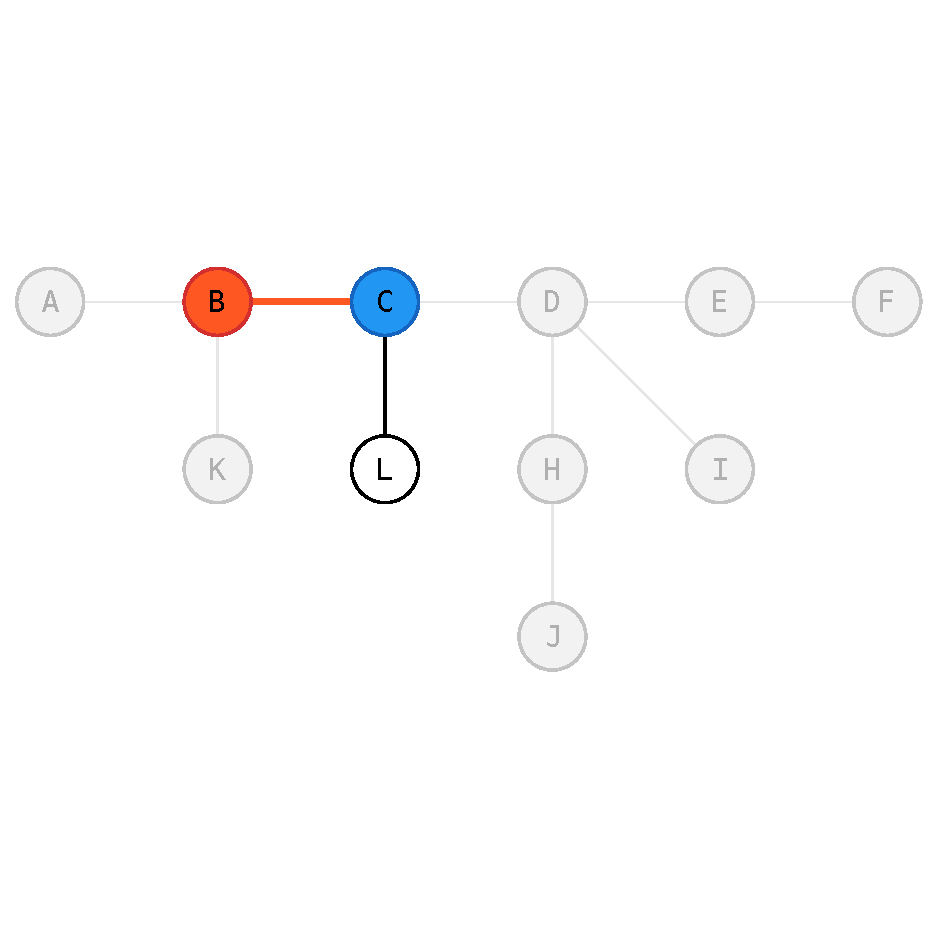
\includegraphics[width=0.28\textwidth]{python/lec06/pruefer/pruefer-9.pdf}\\[2pt]{\scriptsize Шаг 9. $B \to$ код: $C$}} &
\shortstack{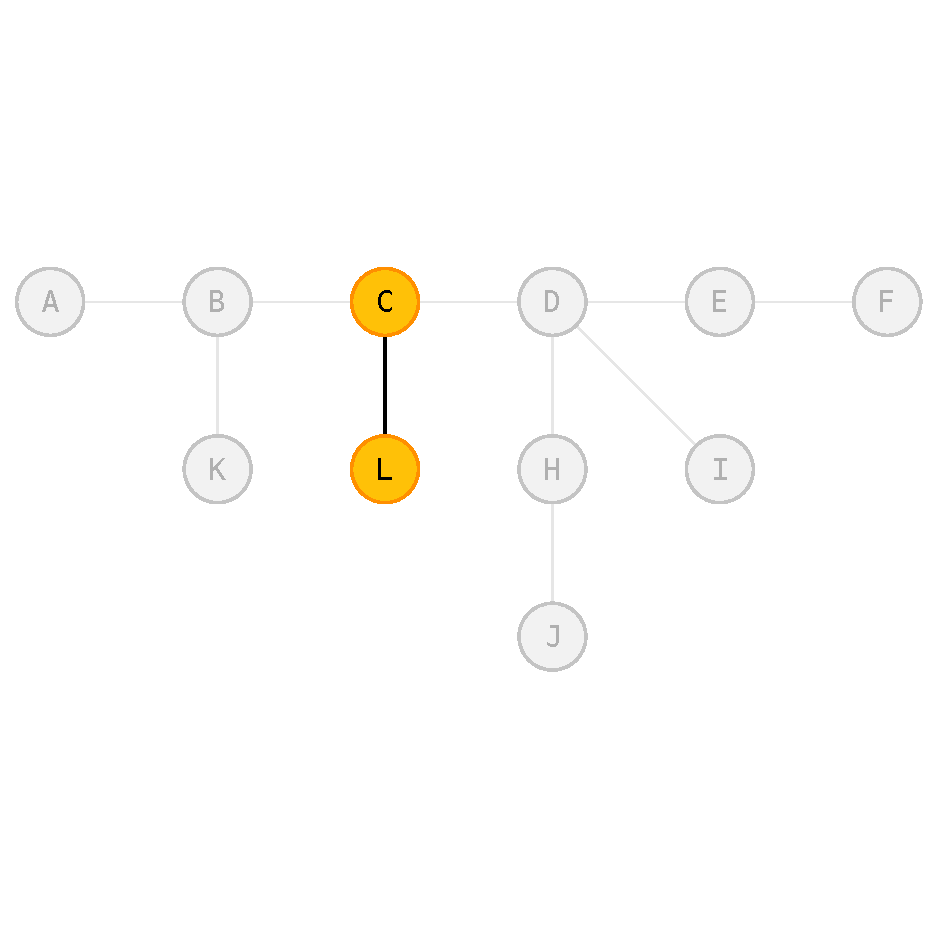
\includegraphics[width=0.28\textwidth]{python/lec06/pruefer/pruefer-10.pdf}\\[2pt]{\scriptsize Шаг 10. Остались $C$ и $L$ --- стоп}} \\
\end{tabular}\end{center}
\end{algo}

% ============================================================
\begin{task}{Код Прюфера: прямая и обратная задача}{pruffer-task}
\textbf{Условие.} \textbf{(а)} Постройте код Прюфера для дерева на вершинах
$1,\dots,6$ с рёбрами $1\!-\!3,\ 2\!-\!3,\ 3\!-\!4,\ 4\!-\!5,\ 4\!-\!6$.
\textbf{(б)} Восстановите дерево по коду Прюфера $(3,3,4,4)$.

\begin{center}
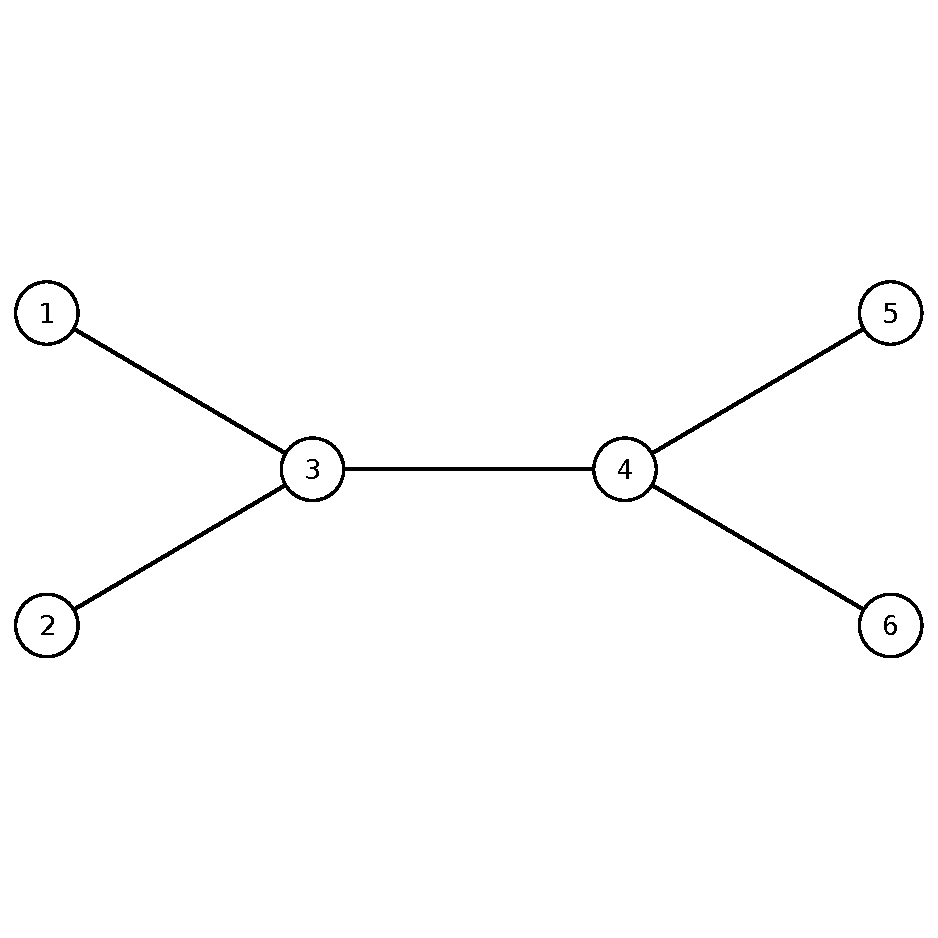
\includegraphics[width=0.45\textwidth]{figures/task-pruefer-1.pdf}
\end{center}

\smallskip
\textbf{Решение (а).} На каждом шаге удаляем лист с наименьшим номером и
записываем номер его единственного соседа; повторяем, пока не останется $2$
вершины (для дерева на $n$ вершинах код имеет длину $n-2=4$).
\begin{enumerate}
  \item Листья $\{1,2,5,6\}$. Наименьший --- $1$, сосед $3$. Записываем $3$.
  \item Листья $\{2,5,6\}$. Наименьший --- $2$, сосед $3$. Записываем $3$.
  \item Теперь $3$ стала листом (соединена только с $4$). Листья $\{3,5,6\}$.
        Наименьший --- $3$, сосед $4$. Записываем $4$.
  \item Листья $\{5,6\}$. Наименьший --- $5$, сосед $4$. Записываем $4$.
        Осталось $2$ вершины ($4$ и $6$) --- стоп.
\end{enumerate}
Код Прюфера: $(3,3,4,4)$.

\smallskip
\textbf{Решение (б).} Обратный алгоритм. Список степеней: каждая вершина
встречается в коде $(\deg-1)$ раз, поэтому степень $=$ (число вхождений в код)
$+1$. Для кода $(3,3,4,4)$ и вершин $1\dots6$:
\[
  \deg 3=3,\ \deg 4=3,\ \deg 1=\deg 2=\deg 5=\deg 6=1.
\]
На каждом шаге берём наименьший лист (вершину степени $1$, не входящую в
оставшийся код) и соединяем с первым элементом кода:
\begin{enumerate}
  \item Код $(3,3,4,4)$; наименьший лист $1$ $\to$ ребро $1\!-\!3$; убираем $3$ из кода.
  \item Код $(3,4,4)$; наименьший лист $2$ $\to$ ребро $2\!-\!3$; убираем $3$.
  \item Код $(4,4)$; теперь $3$ стала листом, наименьший лист $3$ $\to$ ребро $3\!-\!4$; убираем $4$.
  \item Код $(4)$; наименьший лист $5$ $\to$ ребро $5\!-\!4$; убираем $4$.
  \item Код пуст; остались вершины $4$ и $6$ $\to$ ребро $4\!-\!6$.
\end{enumerate}
Восстановленные рёбра: $1\!-\!3,\ 2\!-\!3,\ 3\!-\!4,\ 4\!-\!5,\ 4\!-\!6$ ---
совпадают с исходным деревом из пункта (а) (см. рисунок выше), как и
должно быть.

\textbf{Ответ.} Код Прюфера дерева --- $(3,3,4,4)$; обратное восстановление даёт
то же дерево.
\end{task}

% ============================================================
\begin{task}{Последовательность де Брёйна над алфавитом 0 и 1}{debruijn-task}
\textbf{Условие.} Постройте граф де Брёйна для слов длины $2$ над алфавитом
$\{0,1\}$ и найдите кратчайшую циклическую последовательность, содержащую все
$2$-буквенные слова в качестве подстрок.

\smallskip
\textbf{Решение.} В графе де Брёйна $B(\{0,1\},2)$ вершины --- слова длины $1$
(то есть $0$ и $1$), а дуги --- слова длины $2$: дуга из $u$ в $v$ помечена
словом $uv$. Получаем $4$ дуги:
\[
  0\!\xrightarrow{00}\!0,\quad 0\!\xrightarrow{01}\!1,\quad
  1\!\xrightarrow{11}\!1,\quad 1\!\xrightarrow{10}\!0.
\]

\begin{center}
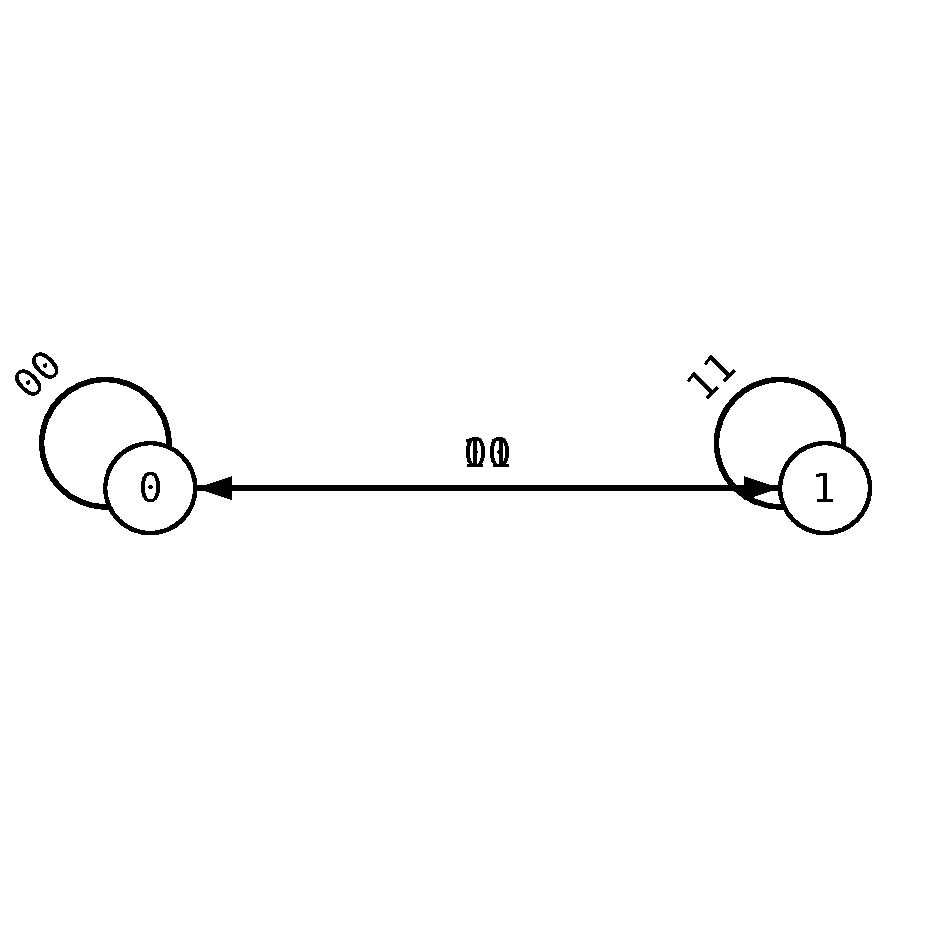
\includegraphics[width=0.35\textwidth]{figures/task-debruijn-1.pdf}
\end{center}
Искомая последовательность --- это \emph{эйлеров цикл} (он проходит по каждой
дуге-слову ровно один раз). У каждой вершины полустепени захода и исхода равны
$2$, граф связен --- эйлеров цикл существует. Один из них:
\[
  0\xrightarrow{00}0\xrightarrow{01}1\xrightarrow{11}1\xrightarrow{10}0,
\]
что даёт циклическую последовательность $\mathbf{0011}$. Читая её по кругу,
получаем все $2$-буквенные слова: $00,\ 01,\ 11,\ 10$.

\textbf{Ответ.} Кратчайшая циклическая последовательность --- $0011$ (длина
$4=2^2$), содержит все четыре слова длины $2$.
\end{task}

% ============================================================
\begin{task}{Гамильтоновость: теорема Дирака}{dirac-task}
\textbf{Условие.} Граф на $5$ вершинах $A,B,C,D,E$ задан как полный граф $K_5$
без двух рёбер $AD$ и $BE$. Является ли он гамильтоновым? Постройте
гамильтонов цикл.

\begin{center}
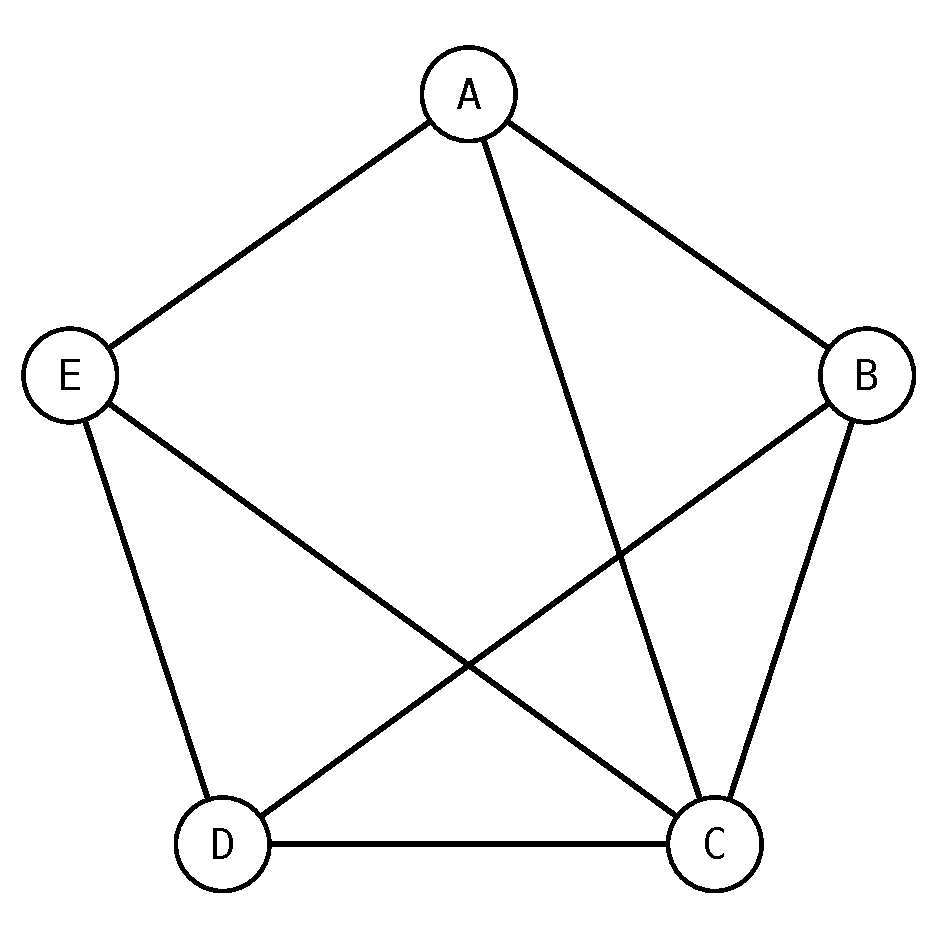
\includegraphics[width=0.35\textwidth]{figures/task-dirac-1.pdf}
\end{center}

\smallskip
\textbf{Решение.} Теорема Дирака: если в графе на $n\geq 3$ вершинах степень
каждой вершины не меньше $n/2$, то граф гамильтонов. Здесь $n=5$, порог
$n/2=2{,}5$. Подсчитаем степени (в $K_5$ каждая вершина имела степень $4$;
удаление $AD$ и $BE$ уменьшает на единицу степени $A,D,B,E$):
\[
  \deg A=\deg B=\deg D=\deg E=3,\qquad \deg C=4.
\]
Все степени $\geq 3>2{,}5$, поэтому по теореме Дирака граф гамильтонов.

Построим гамильтонов цикл, обходя все вершины по одному разу и избегая
отсутствующих рёбер $AD,BE$:
\[
  A\!-\!B\!-\!D\!-\!C\!-\!E\!-\!A.
\]
Проверим рёбра: $AB,\ BD,\ DC,\ CE,\ EA$ --- все присутствуют (среди них нет ни
$AD$, ни $BE$).

\begin{center}
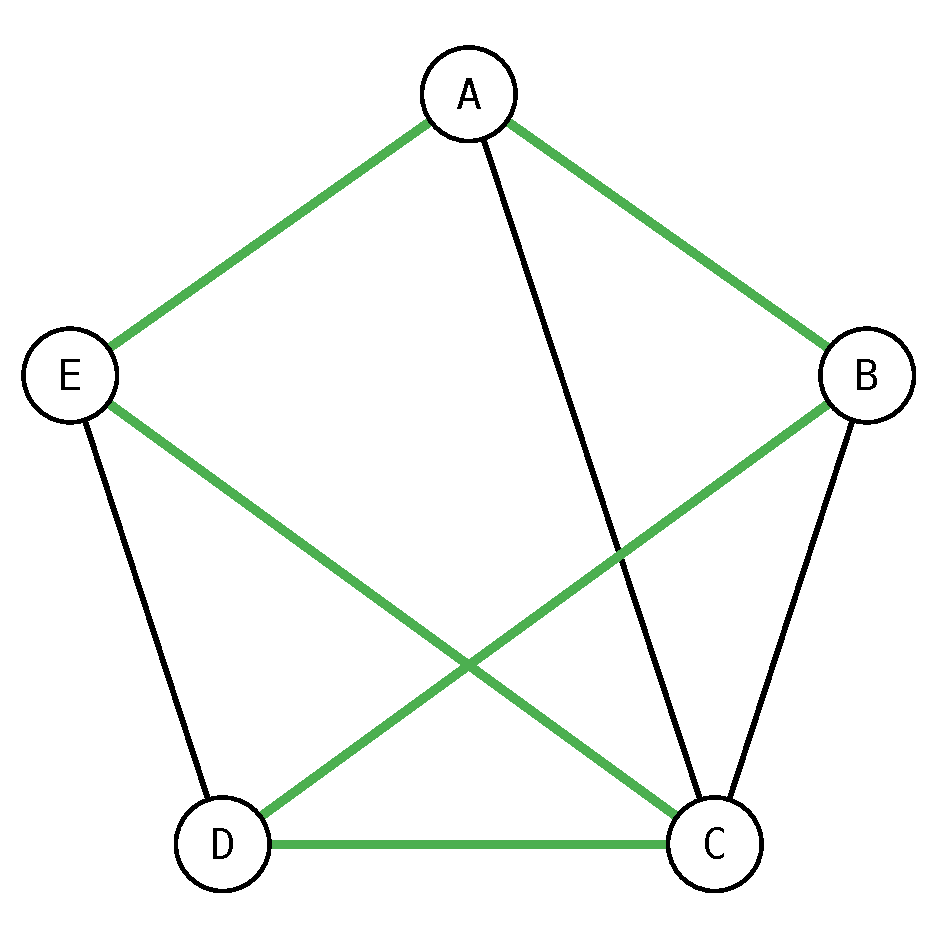
\includegraphics[width=0.35\textwidth]{figures/task-dirac-2.pdf}
\end{center}

\textbf{Ответ.} Граф гамильтонов (условие Дирака выполнено); гамильтонов цикл
$A\!-\!B\!-\!D\!-\!C\!-\!E\!-\!A$.
\end{task}


\chapter{Лекция 7. Код Прюфера (обратная задача). Остовные деревья. Алгоритм Прима}

% ============================================================
% ОБРАТНАЯ ЗАДАЧА КОДА ПРЮФЕРА (стр. 17, dir2 стр. 5)
% ============================================================

\subsection*{Обратная задача кода Прюфера}

\textbf{Дано:}
$V = \{v_1, \ldots, v_n\}$,\quad
$\operatorname{Pruf}(G) = \{v_{i_1}, \ldots, v_{i_{n-2}}\}$.

\textbf{Восстановить} $G$.

\textbf{Step:} выбор $\min$ из $(V \setminus \operatorname{Pruf}(G)) = v_k$; соединяем:
$e = v_k v_{i_s}$, удаляем $v_k$ из $V$, $v_{i_s}$ из $\operatorname{Pruf}(G)$
\quad ($v_{i_s}$ --- $s$-й элемент кода, $s$ --- номер шага).

\textbf{Замечание:} в процессе не обязательно должно быть дерево, а в конце --- обязательно.

% ============================================================
% Пример обратной задачи (стр. 18, dir2 стр. 6)
% ============================================================

\medskip
\noindent\textbf{Пример.}

$V = \{A, B, C, D, E, F, H, I, J\}$,\quad
$\operatorname{Pruf}(G) = \{D, A, A, F, H, A, J\}$.

% Граф: p18-example-1.graph
\grfig{figures/p18-example-1.pdf}{Обратная задача Прюфера}

% ============================================================
% ТЕОРЕМА КЭЛИ (стр. 18, dir2 стр. 6)
% ============================================================

\subsection*{Теорема Кэли}

$V = \{v_1, \ldots, v_n\}$; сколько $\exists$ различных помеченных деревьев?

$|\operatorname{Pruf}(G)| = n - 2 \;\Rightarrow\; n^{n-2}$ помеченных деревьев.

\begin{statement}{Теорема Кэли (о количестве помеченных деревьев)}{cayley}
Количество различных помеченных деревьев на $n$ вершинах равно $n^{n-2}$.
\end{statement}

\begin{proof}
Построим биекцию между помеченными деревьями на $n$ вершинах и
последовательностями длины $n - 2$ из элементов $V$ --- это в точности
код Прюфера.

\textbf{Код корректно определён.} Прямой алгоритм (лекция 6) на каждом
шаге удаляет минимальный лист (у дерева с $\ge 2$ вершинами лист всегда
есть) и делает ровно $n - 2$ записи --- любому дереву отвечает ровно одна
последовательность $\operatorname{Pruf}(G) \in V^{n-2}$.

\textbf{Инъективность и сюръективность.} Обратный алгоритм (выше) по
\emph{любой} последовательности $p \in V^{n-2}$ строит граф: на каждом
шаге к минимальной вершине, не встречающейся в остатке кода и ещё не
использованной, проводится ребро к первому элементу кода. Получается
ровно $n - 1$ ребро, и построенный граф связен и ацикличен (каждый шаг
присоединяет <<новый лист>> к остальной части), т.\,е. дерево. Прямой
проверкой видно, что обратный алгоритм восстанавливает исходное дерево
по его коду, а прямой алгоритм, применённый к дереву, построенному по
последовательности $p$, возвращает $p$. Значит, соответствие ---
биекция.

Последовательностей длины $n - 2$ из $n$ символов ровно $n^{n-2}$,
следовательно, столько же и помеченных деревьев.
\end{proof}

% ============================================================
% РЁБЕРНО-ВЗВЕШЕННЫЕ ГРАФЫ. MIN ОСТОВНОЕ ДЕРЕВО (стр. 18, dir2 стр. 6)
% ============================================================

\subsection*{Рёберно-взвешенные графы. Минимальное остовное дерево}

\begin{defn}{Рёберно-взвешенный граф}{weighted-graph}
$G(V, E)$ --- (рёберно-)взвешенный:

$\exists\, \sigma\colon E \to W$,

где $W$ --- некоторое упорядоченное мн-во
с операциями, зависящими от задачи.

\textbf{NB:} $W$ --- нижняя упорядоченная мн-во.
\end{defn}

$G(V, E)$ --- неориент., н.\,у.\,о. --- связный.

$\sigma\colon E \to \mathbb{R}$.

\begin{defn}{Остов (каркас)}{spanning-tree-def}
\textbf{Остов} (скелет, каркас) --- связный подграф в $G$, являющийся деревом и содержащий все вершины $G$.
\end{defn}

\begin{defn}{Остовное дерево}{spanning-tree}
$G(V, E)$ --- \textbf{остовное дерево} $G$: $T$ --- дерево и остов.

Если граф --- не дерево, то остовов несколько.
\end{defn}

% Пример: треугольник — 3 остова

\begin{defn}{Минимальное остовное дерево}{mst}
$G(V, E)$ --- связный, взвешенный.

$\sigma\colon E \to \mathbb{R}$.

Минимальное остовное дерево $G$:
$T_G\colon \displaystyle\sum_{\substack{(v,\hat{v}) \in T \\ e \in \hat{E}}} \sigma(e) \longrightarrow \min$
по всем $T$ для $G$.
\end{defn}

% ============================================================
% Жадные алгоритмы (стр. 19, dir2 стр. 7)
% ============================================================

\medskip
\textbf{Жадные алгоритмы} --- алгоритмы, оптимальные только в рамках одного шага.

% Пример контрпримера жадности:
% Граф: p19-example-1.graph
\grfig{figures/p19-example-1.pdf}{Жадный алг.: контрпример 1}

% Ещё пример:
% Граф: p19-example-2.graph
\grfig{figures/p19-example-2.pdf}{Жадный алг.: контрпример 2}

% ============================================================
% АЛГОРИТМ ПРИМА (стр. 19, dir2 стр. 7)
% ============================================================

\subsection*{Алгоритм построения min остовного дерева}

$G(V, E)$, $\sigma\colon E \to \mathbb{R}$, н.\,у.\,о. --- связный.

\begin{algo}{Алгоритм Прима}{prim}

\textbf{Инициализация:} $\operatorname{start} \in V$ (любая вершина);
дерево $T = \{\operatorname{start}\}$.

\textbf{Step:} среди всех рёбер, соединяющих уже выбранную вершину с ещё
не выбранной, берём ребро $e$ с минимальным весом $\sigma(e)$; добавляем
его (и новую вершину) в $T$. Новая вершина присоединяется не обязательно
к последней --- к \emph{любой} из уже выбранных. Повторяем, пока $T$ не
охватит все вершины ($n - 1$ ребро).

\medskip
\noindent\textbf{Пример} (старт из $J$):

% Граф: p19-prim-example-1.graph
\grfig[0.55]{figures/p19-prim-example-1.pdf}{Алг. Прима: взвешенный граф 9 вершин}

\medskip
\begin{center}
\begin{tabular}{c|c|c|l}
$V$ & $e$ & $\sum \sigma(e)$ & комментарий \\ \hline
$J$  & ---     & 0  & старт \\
$I$  & $IJ(3)$ & 3  & единственное ребро из $J$ \\
$D$  & $DI(1)$ & 4  & $DI(1) < IF(2)$ \\
$F$  & $IF(2)$ & 6  & $IF(2) < AD(4) < DH(5) = DF(5) < \ldots$ \\
$A$  & $AD(4)$ & 10 & $AD(4) < DH(5) < FH(6) < \ldots$ \\
$H$  & $DH(5)$ & 15 & $DH(5) < AB(6) = FH(6) < DC(7)$ \\
$B$  & $AB(6)$ & 21 & $AB(6) < DC(7) < BD(9)$ \\
$C$  & $BC(1)$ & 22 & после прихода $B$ открылось ребро $BC(1)$ \\
$E$  & $CE(8)$ & 30 & единственное ребро к последней вершине $E$ \\
\end{tabular}
\end{center}

\medskip
Минимальное остовное дерево: $IJ, DI, IF, AD, DH, AB, BC, CE$;
суммарный вес $\sum \sigma = 30$.

\medskip
\noindent\textbf{Работа алгоритма по шагам} (выбранные рёбра --- зелёные,
текущее добавляемое --- оранжевое, недоступные пока рёбра --- серые):

\begin{center}\begin{tabular}{ccc}
\shortstack{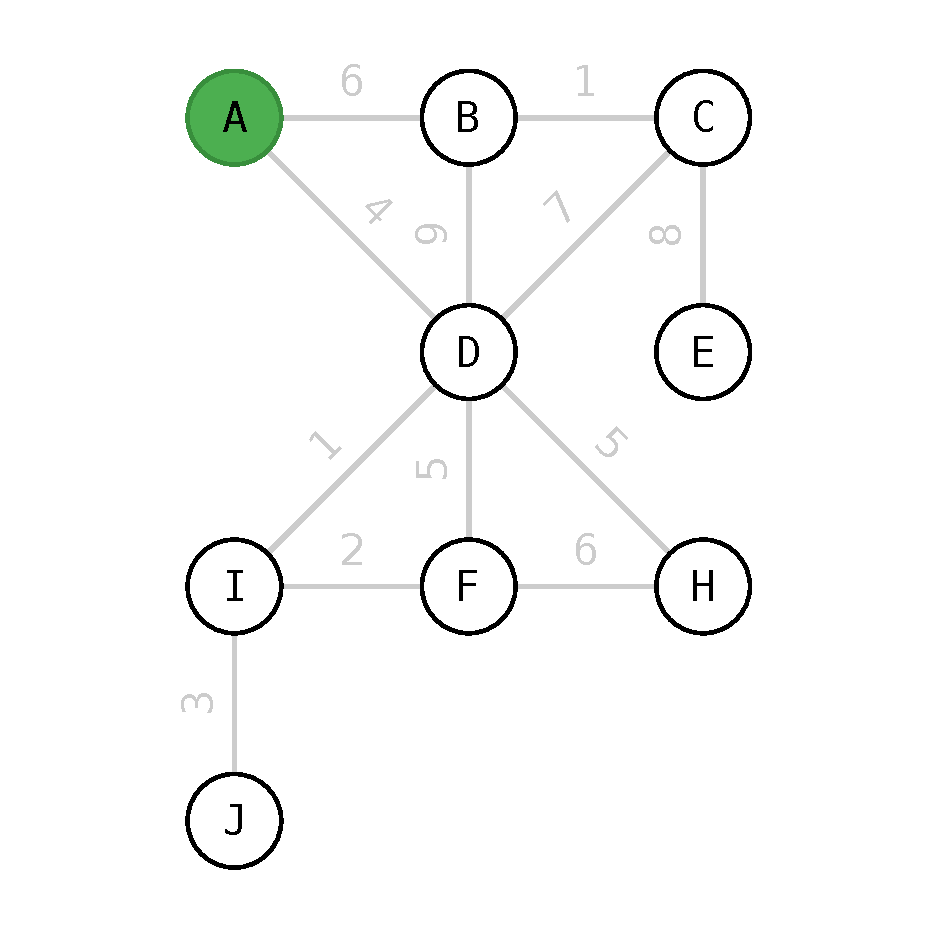
\includegraphics[width=0.30\textwidth]{python/lec07/prim/prim-0.pdf}\\[2pt]{\scriptsize Шаг 0. Старт: $T=\{J\}$}} &
\shortstack{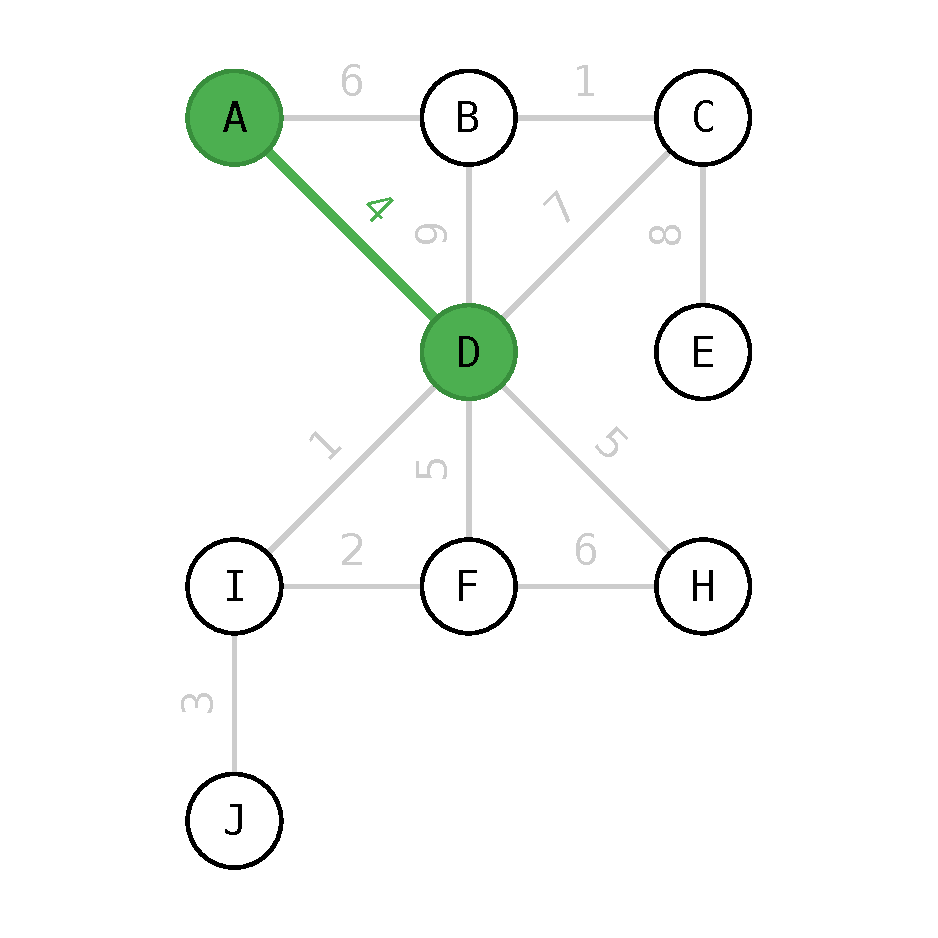
\includegraphics[width=0.30\textwidth]{python/lec07/prim/prim-1.pdf}\\[2pt]{\scriptsize Шаг 1. $+IJ(3)$, $\Sigma=3$}} &
\shortstack{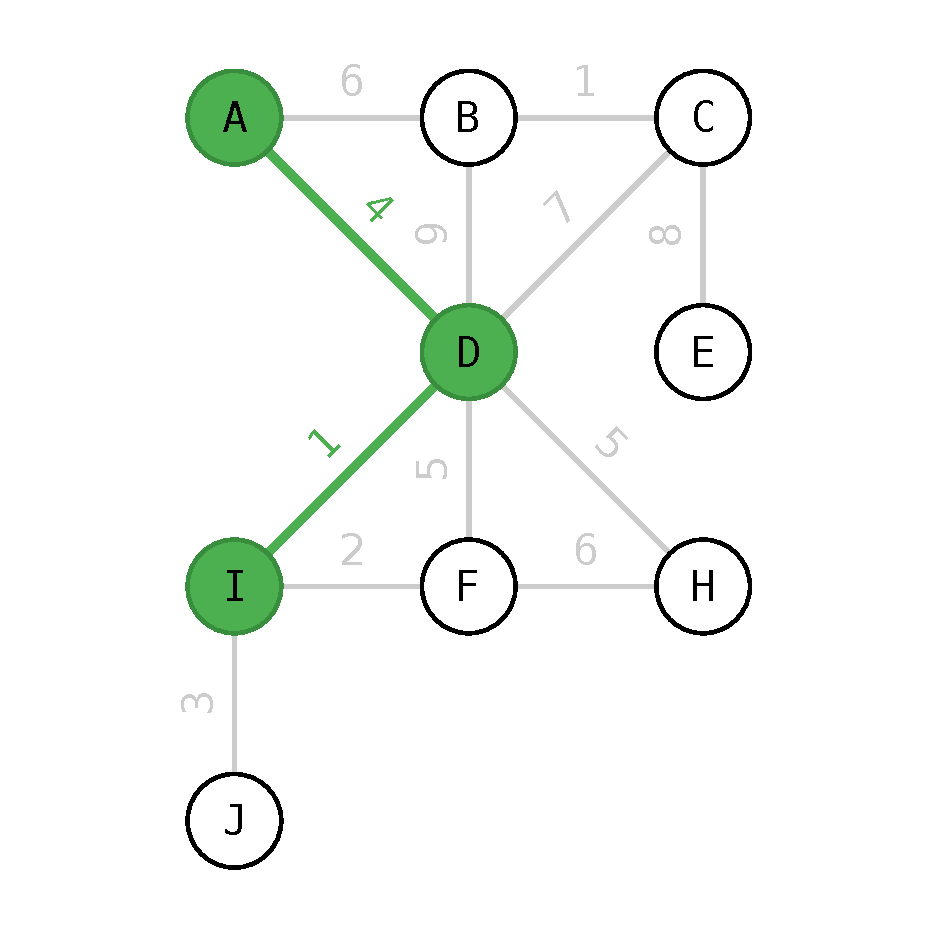
\includegraphics[width=0.30\textwidth]{python/lec07/prim/prim-2.pdf}\\[2pt]{\scriptsize Шаг 2. $+DI(1)$, $\Sigma=4$}} \\
\end{tabular}\end{center}
\begin{center}\begin{tabular}{ccc}
\shortstack{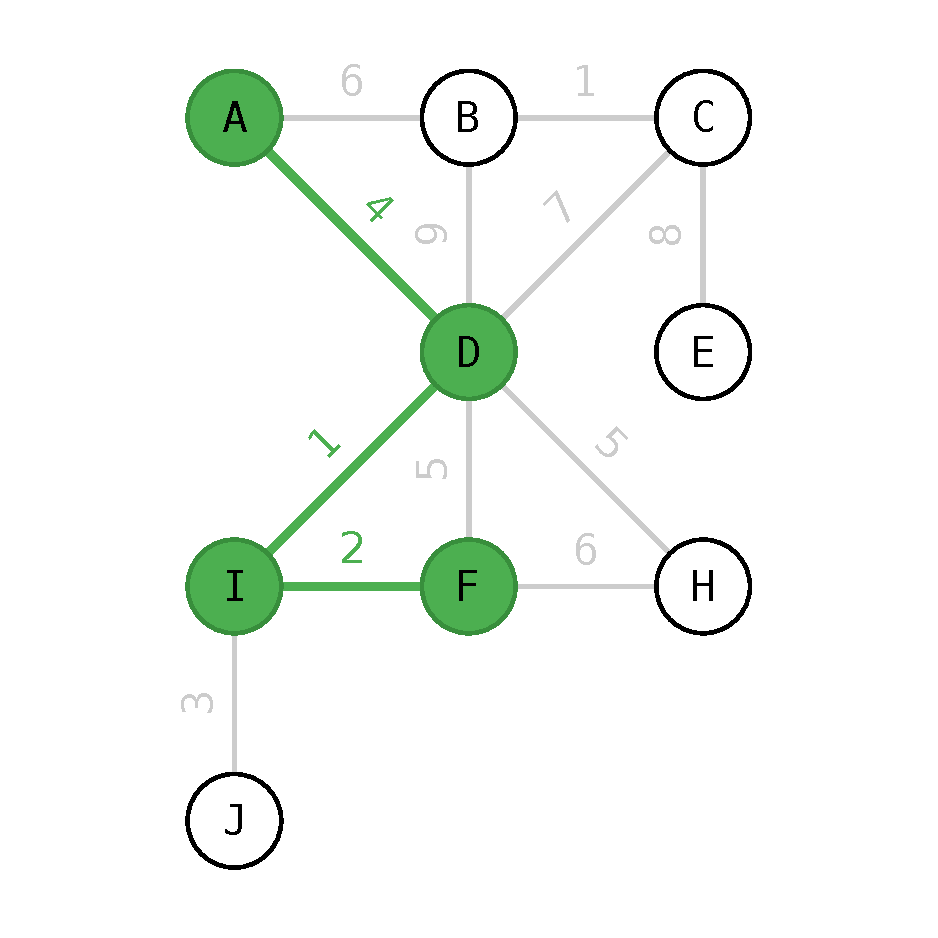
\includegraphics[width=0.30\textwidth]{python/lec07/prim/prim-3.pdf}\\[2pt]{\scriptsize Шаг 3. $+IF(2)$, $\Sigma=6$}} &
\shortstack{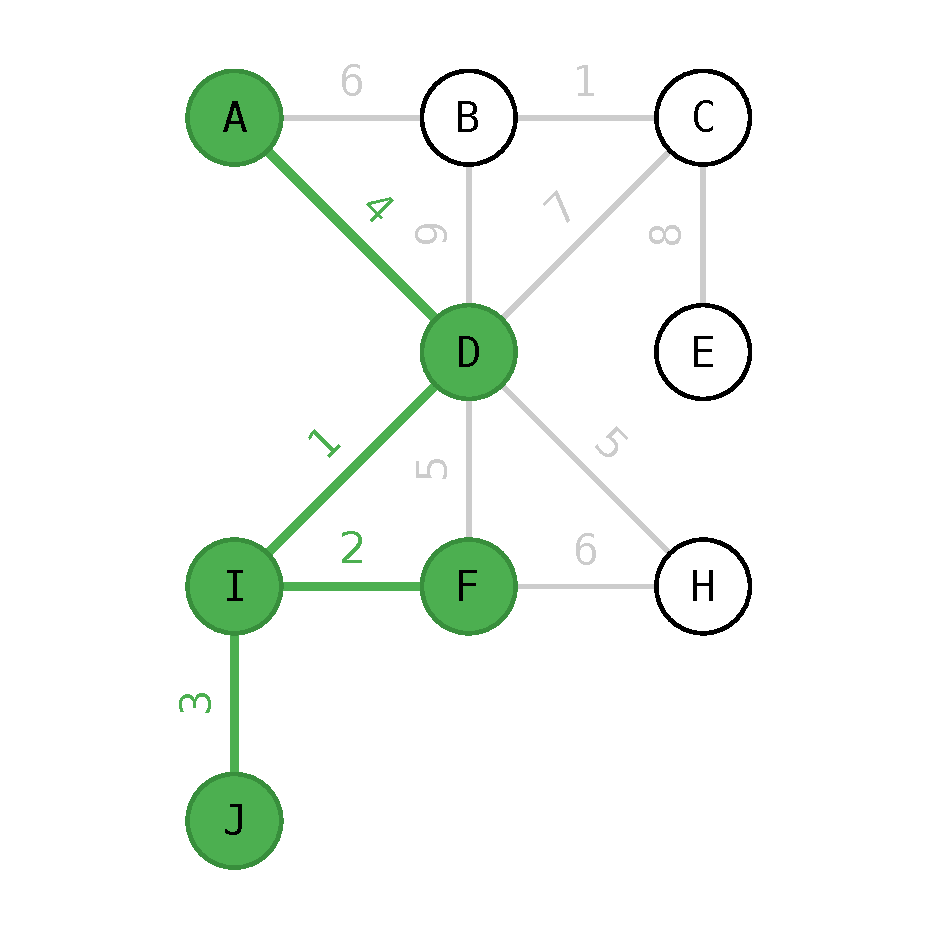
\includegraphics[width=0.30\textwidth]{python/lec07/prim/prim-4.pdf}\\[2pt]{\scriptsize Шаг 4. $+AD(4)$, $\Sigma=10$}} &
\shortstack{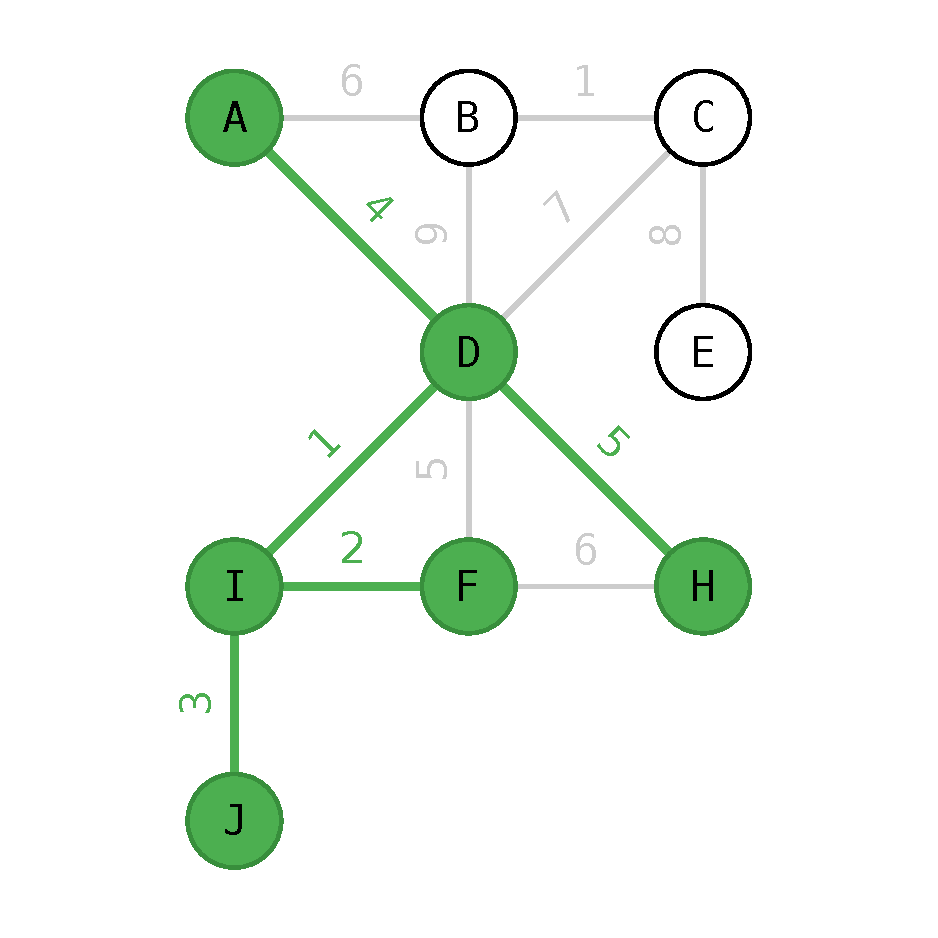
\includegraphics[width=0.30\textwidth]{python/lec07/prim/prim-5.pdf}\\[2pt]{\scriptsize Шаг 5. $+DH(5)$, $\Sigma=15$}} \\
\end{tabular}\end{center}
\begin{center}\begin{tabular}{ccc}
\shortstack{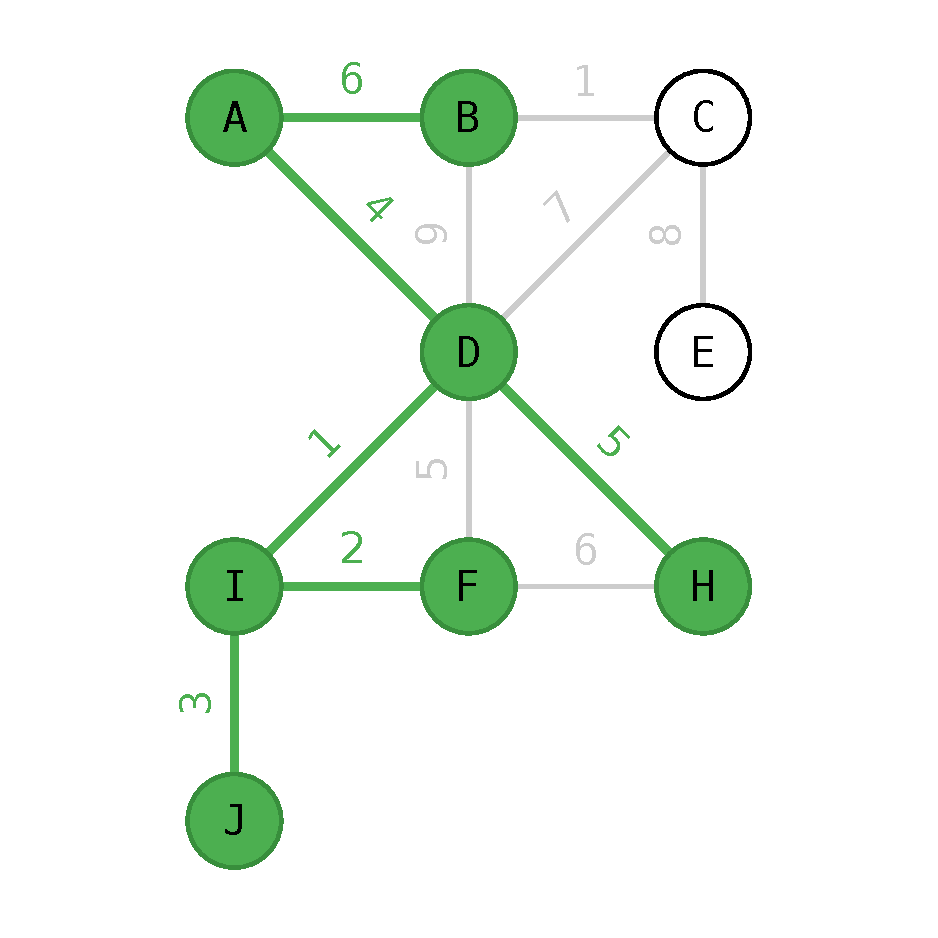
\includegraphics[width=0.30\textwidth]{python/lec07/prim/prim-6.pdf}\\[2pt]{\scriptsize Шаг 6. $+AB(6)$, $\Sigma=21$}} &
\shortstack{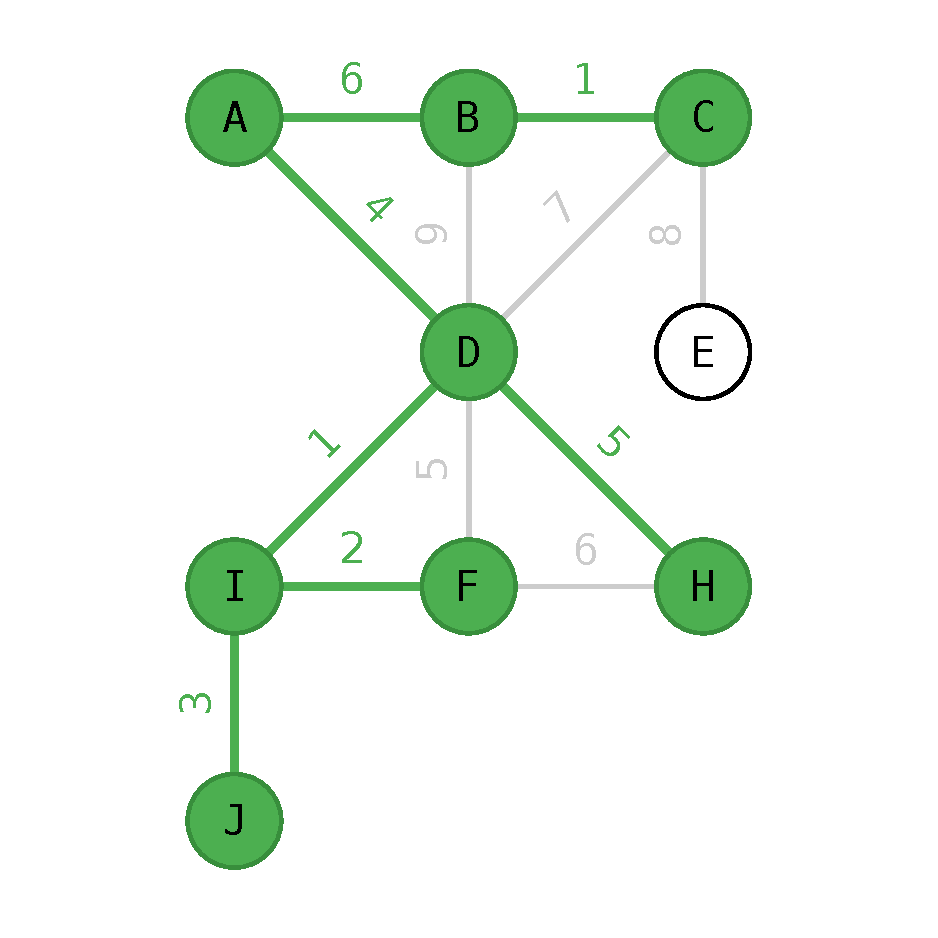
\includegraphics[width=0.30\textwidth]{python/lec07/prim/prim-7.pdf}\\[2pt]{\scriptsize Шаг 7. $+BC(1)$, $\Sigma=22$}} &
\shortstack{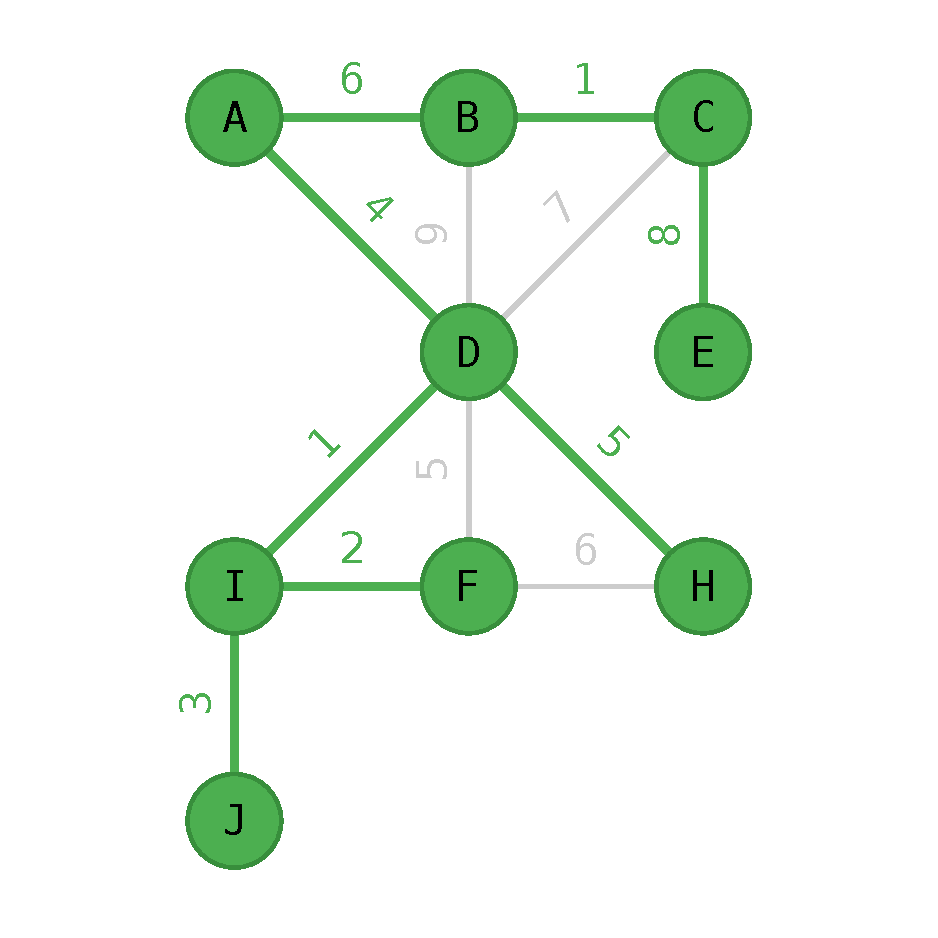
\includegraphics[width=0.30\textwidth]{python/lec07/prim/prim-8.pdf}\\[2pt]{\scriptsize Шаг 8. $+CE(8)$, $\Sigma=30$}} \\
\end{tabular}\end{center}
\begin{center}
\shortstack{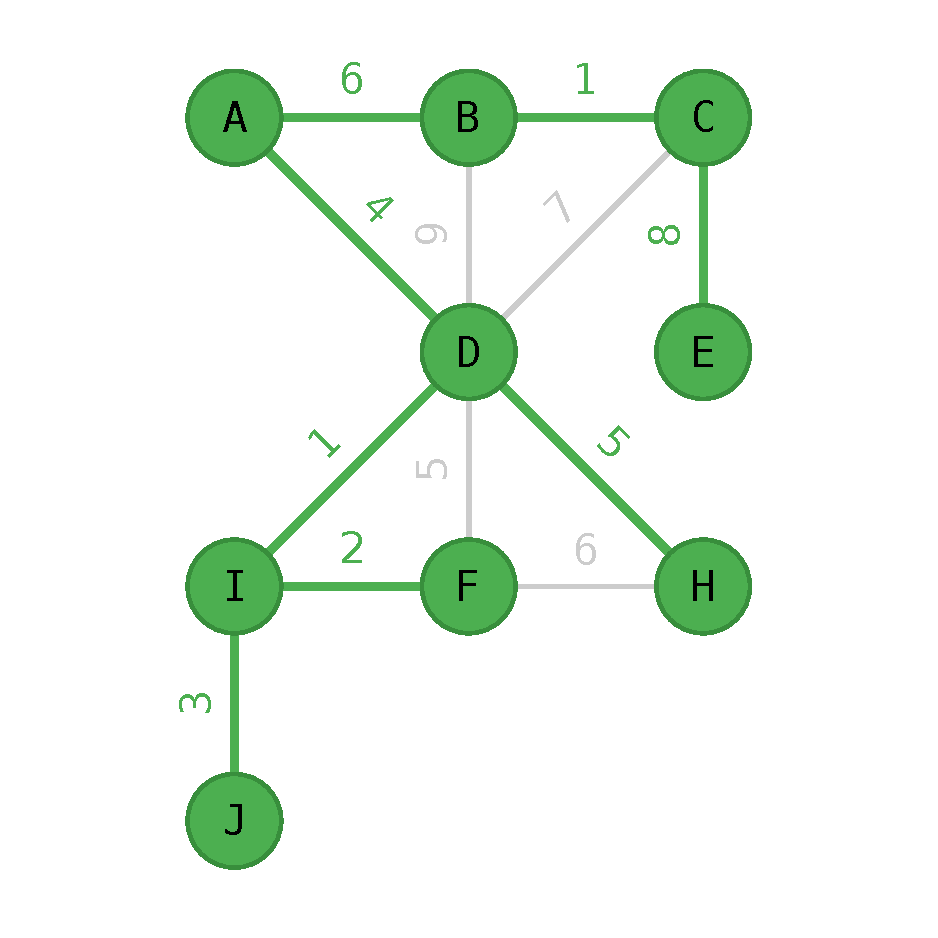
\includegraphics[width=0.32\textwidth]{python/lec07/prim/prim-9.pdf}\\[2pt]{\scriptsize Шаг 9. Остов построен, $\Sigma = 30$}}
\end{center}

\medskip
\textbf{Замечание.} Если все веса рёбер различны, минимальное остовное
дерево единственно --- и алгоритм Прима находит именно его независимо
от выбора стартовой вершины.
\end{algo}

% ============================================================
\begin{task}{Минимальное остовное дерево: алгоритм Прима}{prim-task}
\textbf{Условие.} Дан неориентированный взвешенный граф на вершинах
$A,B,C,D,E,F$ с рёбрами
\[
  AB=4,\quad AC=2,\quad BC=5,\quad BD=10,\quad CE=3,\quad ED=6,\quad EF=7,\quad DF=11.
\]
Постройте минимальное остовное дерево алгоритмом Прима, начиная с вершины $A$.
Укажите порядок включения рёбер и суммарный вес.

\begin{center}
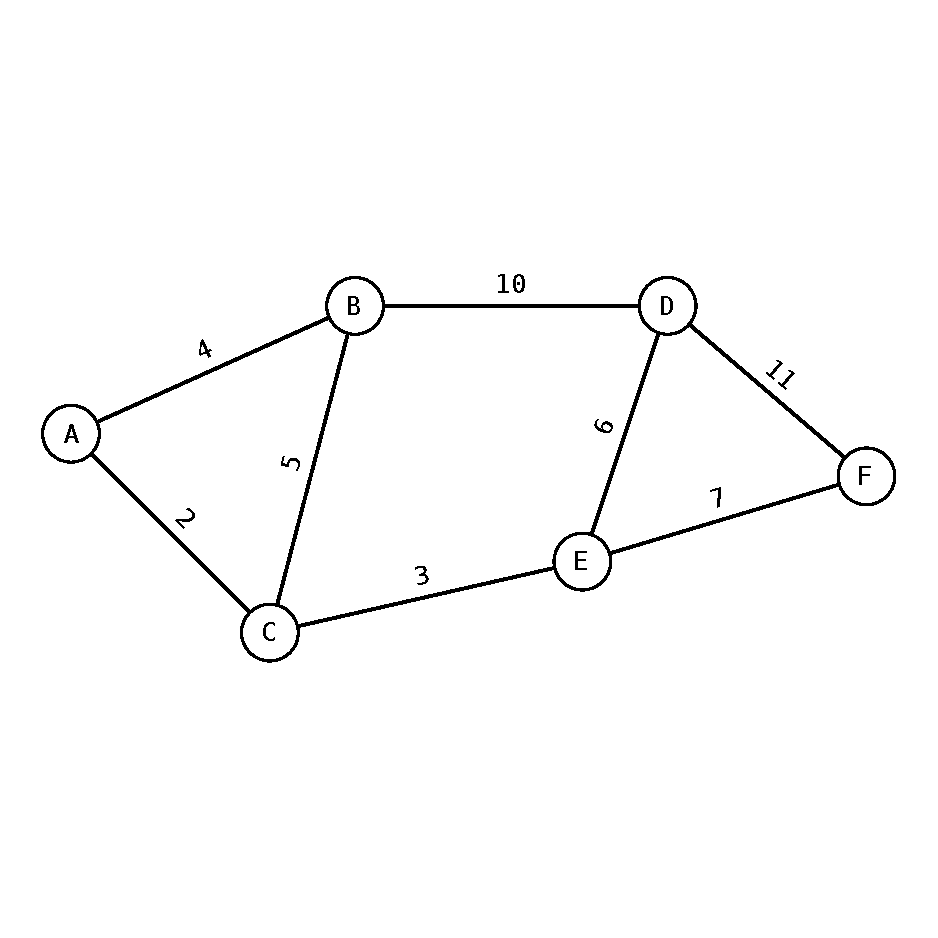
\includegraphics[width=0.5\textwidth]{figures/task-prim-1.pdf}
\end{center}

\textbf{Решение.} Алгоритм Прима выращивает дерево из одной вершины, добавляя на
каждом шаге ребро наименьшего веса, ведущее из уже построенного дерева в ещё не
включённую вершину.
\begin{enumerate}
  \item Дерево $\{A\}$. Из $A$ выходят $AC=2$ и $AB=4$; минимум --- $AC=2$,
        включаем вершину $C$.
  \item Дерево $\{A,C\}$. Доступны $CE=3,\ AB=4,\ BC=5$; минимум --- $CE=3$,
        включаем $E$.
  \item Дерево $\{A,C,E\}$. Доступны $AB=4,\ BC=5,\ ED=6,\ EF=7$;
        минимум --- $AB=4$, включаем $B$.
  \item Дерево $\{A,C,E,B\}$. Доступны $ED=6,\ EF=7,\ BD=10$;
        минимум --- $ED=6$, включаем $D$.
  \item Дерево $\{A,C,E,B,D\}$. Доступны $EF=7,\ DF=11$; минимум --- $EF=7$,
        включаем $F$. Дерево охватило все вершины.
\end{enumerate}
Порядок включения рёбер: $AC(2),\ CE(3),\ AB(4),\ ED(6),\ EF(7)$.

\medskip
\noindent Шаги построения:

\begin{center}\begin{tabular}{ccc}
\shortstack{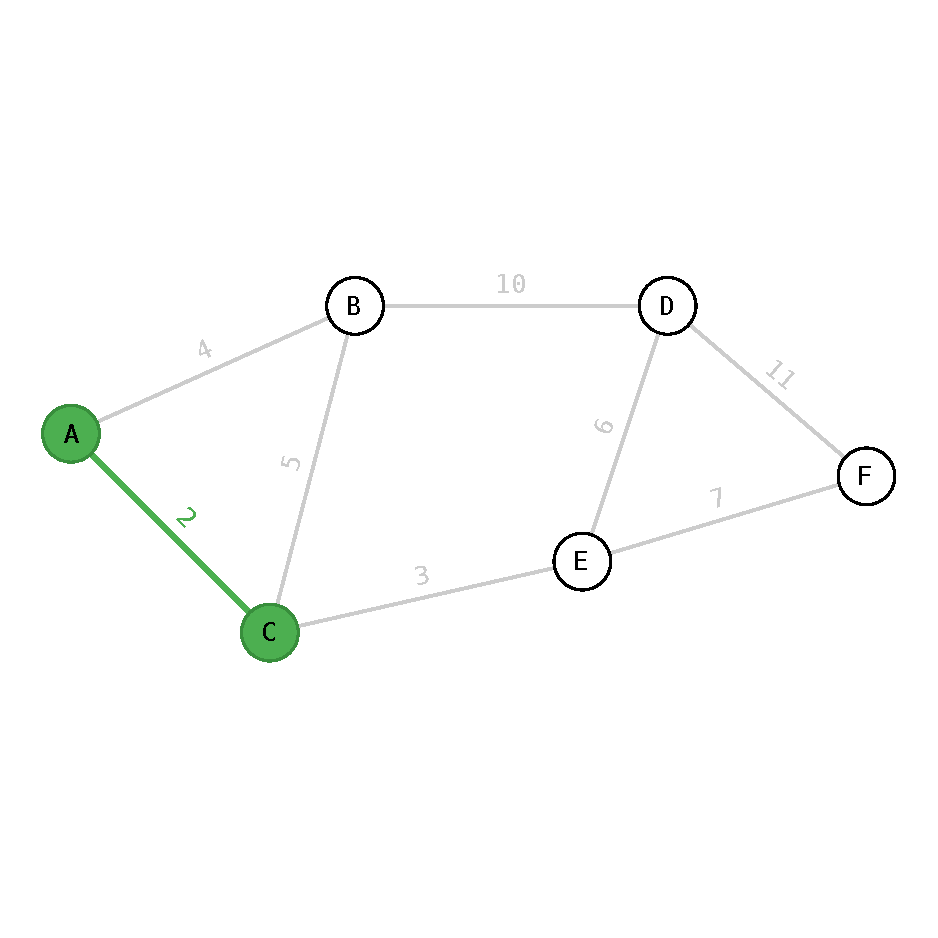
\includegraphics[width=0.30\textwidth]{python/lec07/prim_task/primt-1.pdf}\\[2pt]{\scriptsize $+AC(2)$}} &
\shortstack{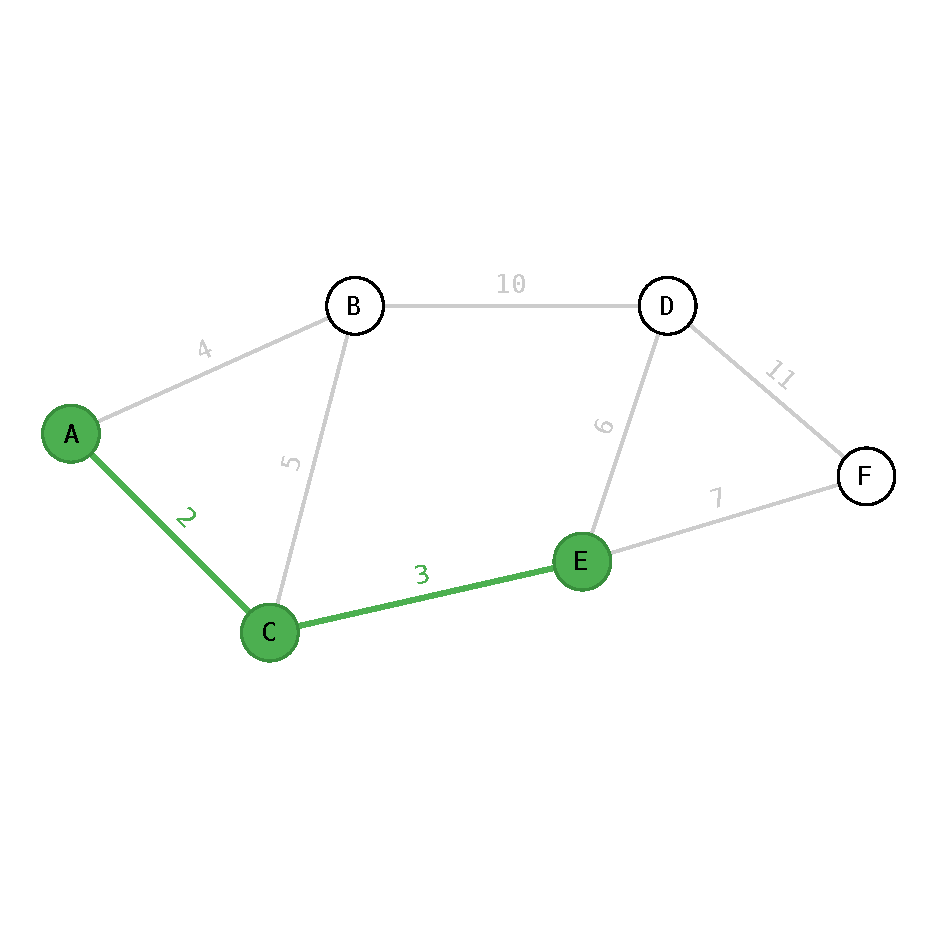
\includegraphics[width=0.30\textwidth]{python/lec07/prim_task/primt-2.pdf}\\[2pt]{\scriptsize $+CE(3)$}} &
\shortstack{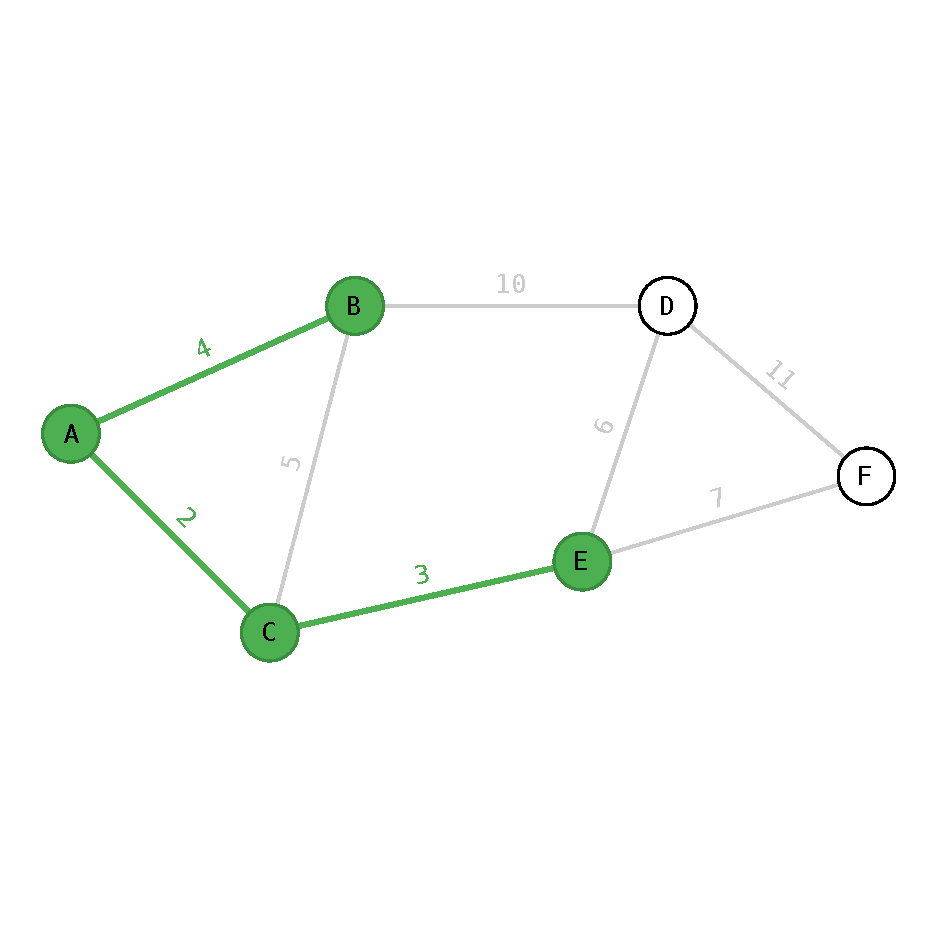
\includegraphics[width=0.30\textwidth]{python/lec07/prim_task/primt-3.pdf}\\[2pt]{\scriptsize $+AB(4)$}} \\
\end{tabular}\end{center}
\begin{center}\begin{tabular}{ccc}
\shortstack{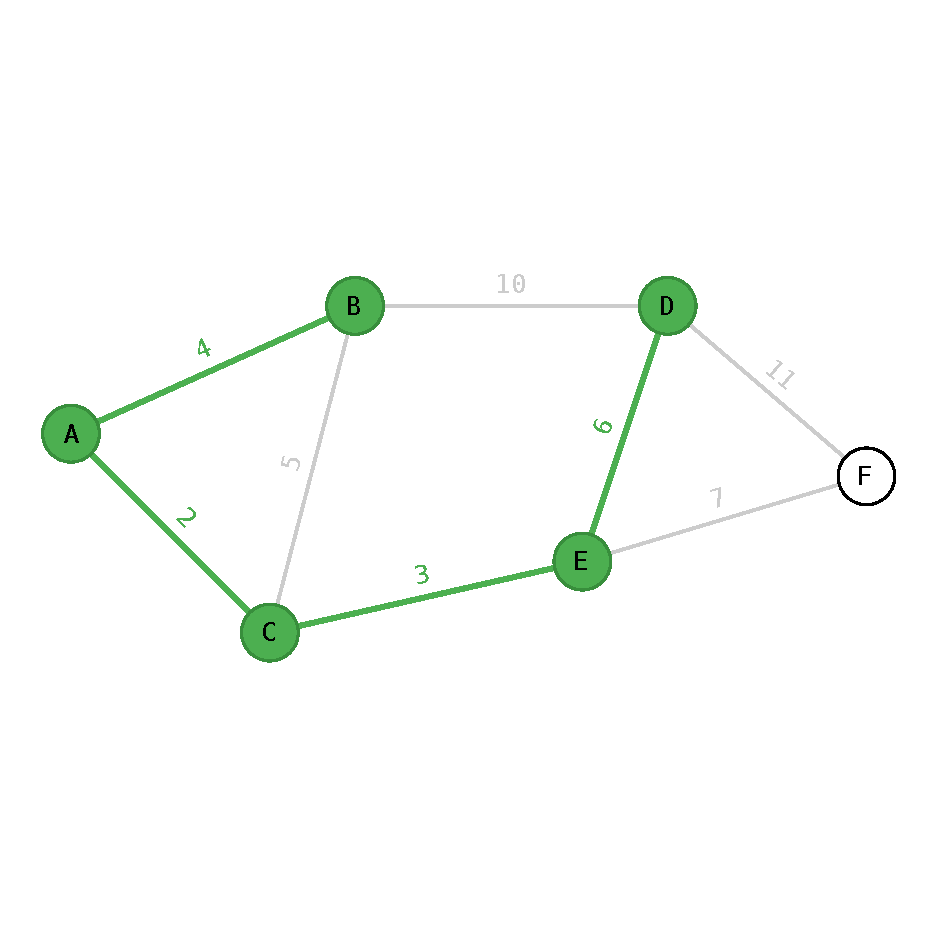
\includegraphics[width=0.30\textwidth]{python/lec07/prim_task/primt-4.pdf}\\[2pt]{\scriptsize $+ED(6)$}} &
\shortstack{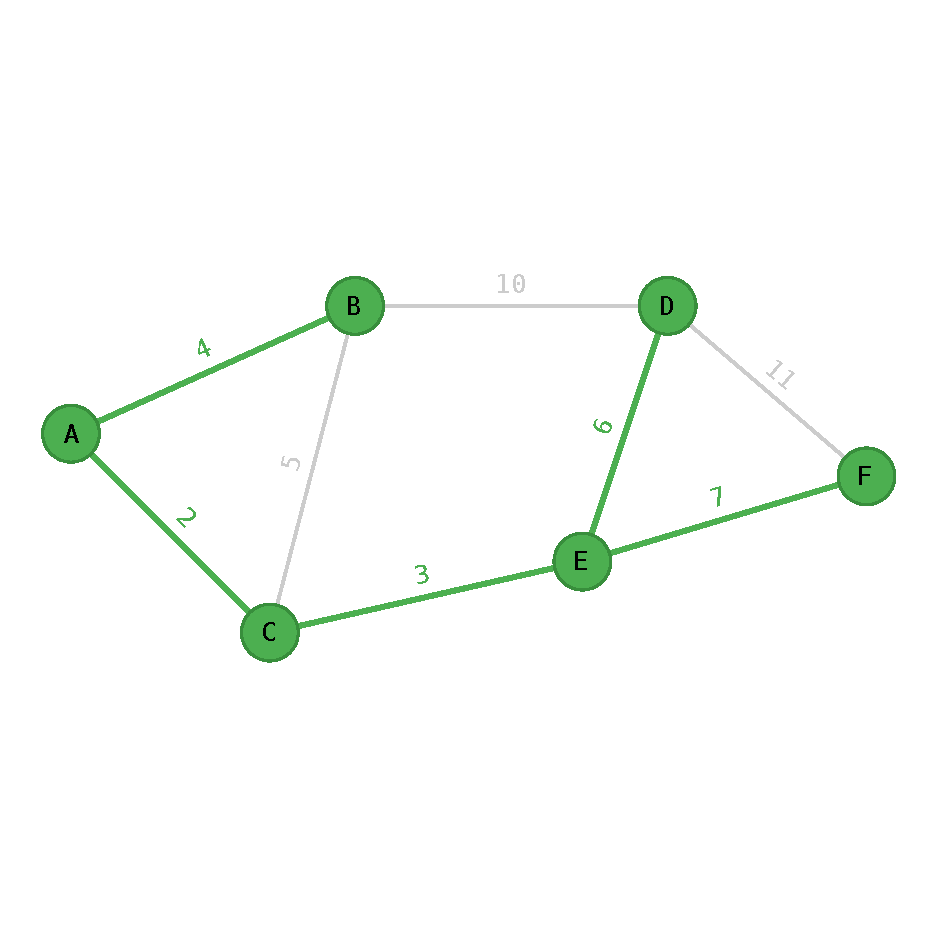
\includegraphics[width=0.30\textwidth]{python/lec07/prim_task/primt-5.pdf}\\[2pt]{\scriptsize $+EF(7)$}} &
\shortstack{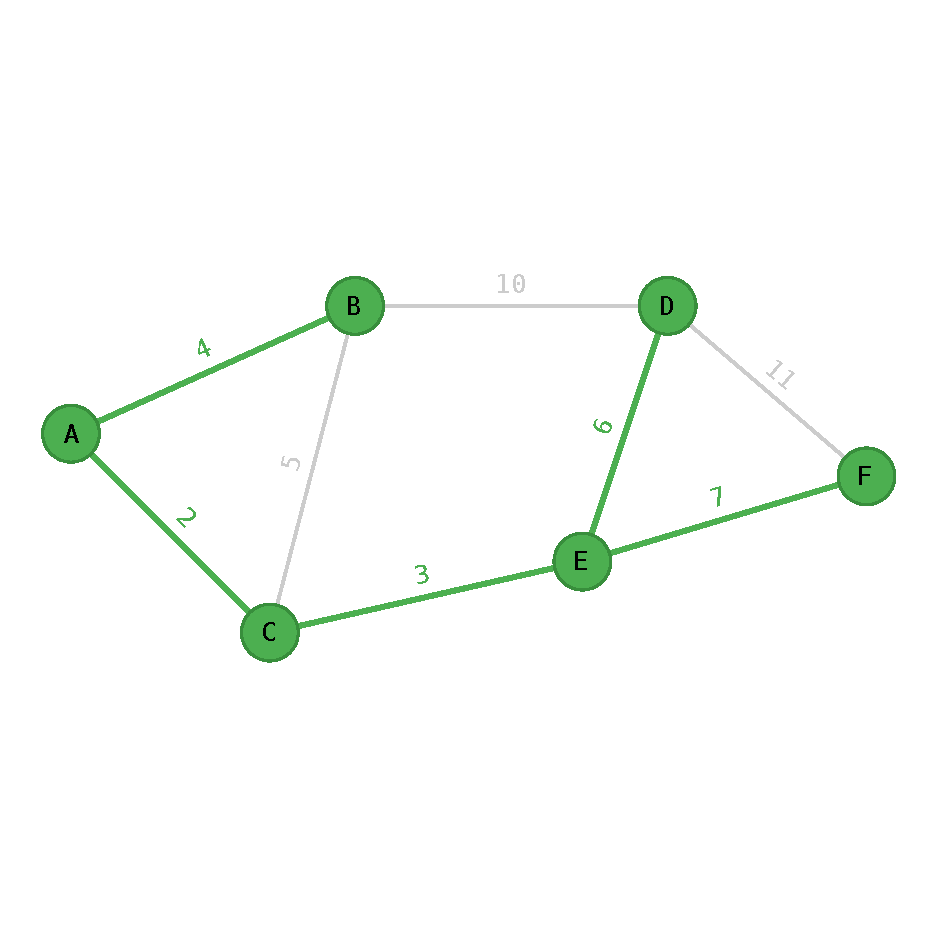
\includegraphics[width=0.30\textwidth]{python/lec07/prim_task/primt-6.pdf}\\[2pt]{\scriptsize Остов построен}} \\
\end{tabular}\end{center}

\textbf{Ответ.} Минимальное остовное дерево состоит из рёбер $AC,CE,AB,ED,EF$;
его суммарный вес равен $2+3+4+6+7=22$.
\end{task}


\chapter{Лекция 8. Алгоритм Краскала. Главные циклы. Цикловое пространство}

% ============================================================
% АЛГОРИТМ КРАСКАЛА
% ============================================================

$G(V, E)$ --- связный, $\sigma\colon E \to \mathbb{R}$.

$\Rightarrow\; T_G(V, \hat{E})$ --- остовное дерево ($\min \sum \sigma(e),\; e \in \hat{E}$).

\begin{algo}{Алгоритм Краскала}{kruskal}

\textbf{Step:} рёбра перебираются в порядке возрастания веса; очередное
ребро $e$ с минимальным $\sigma(e)$ добавляется в остов, если при этом
\emph{не появляется цикл} (т.\,е. концы $e$ лежат в разных компонентах
уже построенного леса); иначе ребро пропускается.

\medskip
\noindent\textbf{Пример} (граф той же структуры, что у алгоритма Прима,
с другими весами):

% Граф: p20-kraskal-example-1.graph
\grfig[0.55]{figures/p20-kraskal-example-1.pdf}{Алг. Краскала: взвешенный граф 9 вершин}

\medskip
\begin{center}
\begin{tabular}{c|c|c|l}
$V$ & $e$ & $\sum \sigma(e)$ & комментарий \\ \hline
---     & ---      & 0  & лес из 9 изолированных вершин \\
$J, I$  & $JI(1)$  & 1  & соединяем $\{J\}$ и $\{I\}$ \\
$B, C$  & $BC(2)$  & 3  & соединяем $\{B\}$ и $\{C\}$ \\
$A, D$  & $AD(3)$  & 6  & соединяем $\{A\}$ и $\{D\}$ \\
$H$     & $HD(4)$  & 10 & $H$ присоединяется к $\{A, D\}$ \\
$F$     & $AF(5)$  & 15 & $F$ присоединяется к $\{A, D, H\}$ \\
$E$     & $DE(6)$  & 21 & $E$ присоединяется к $\{A, D, H, F\}$ \\
---     & $JD(7)$  & 28 & сливаем $\{J, I\}$ и $\{A, D, H, F, E\}$ \\
---     & $BD(8)$  & 36 & сливаем $\{B, C\}$ с остальными; $8$ рёбер --- стоп \\
\end{tabular}
\end{center}

\medskip
Оставшиеся рёбра $EC(9)$, $BE(10)$, $AB(11)$, $FH(12)$, $HI(13)$,
$EJ(14)$ замыкали бы циклы и пропускаются. Минимальное остовное дерево:
$JI, BC, AD, HD, AF, DE, JD, BD$, суммарный вес $\sum\sigma = 36$.

\medskip
\textbf{Упр.} Почему алгоритм сойдётся (построит остов)?

\textit{Ответ.} Каждое добавленное ребро уменьшает число компонент леса
ровно на $1$: начали с $|V|$ компонент, дерево получится после $|V| - 1$
добавлений. Застрять алгоритм не может: пока компонент больше одной,
в связном графе обязательно найдётся ребро между разными компонентами
--- и при просмотре списка оно не будет пропущено.

\medskip
\noindent\textbf{Работа алгоритма по шагам} (добавленные рёбра ---
зелёные, текущее --- оранжевое, пропущенные --- бледно-серые):

\begin{center}\begin{tabular}{ccc}
\shortstack{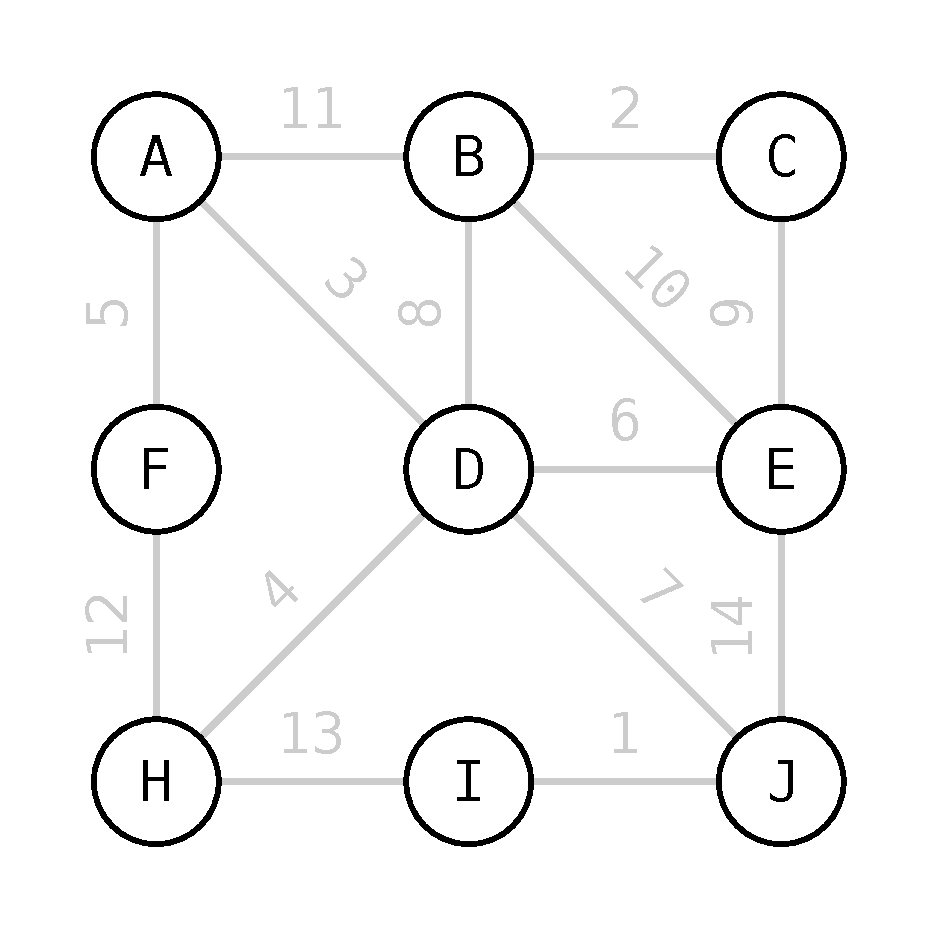
\includegraphics[width=0.30\textwidth]{python/lec08/kruskal/kruskal-0.pdf}\\[2pt]{\scriptsize Шаг 0. Лес из изолированных вершин}} &
\shortstack{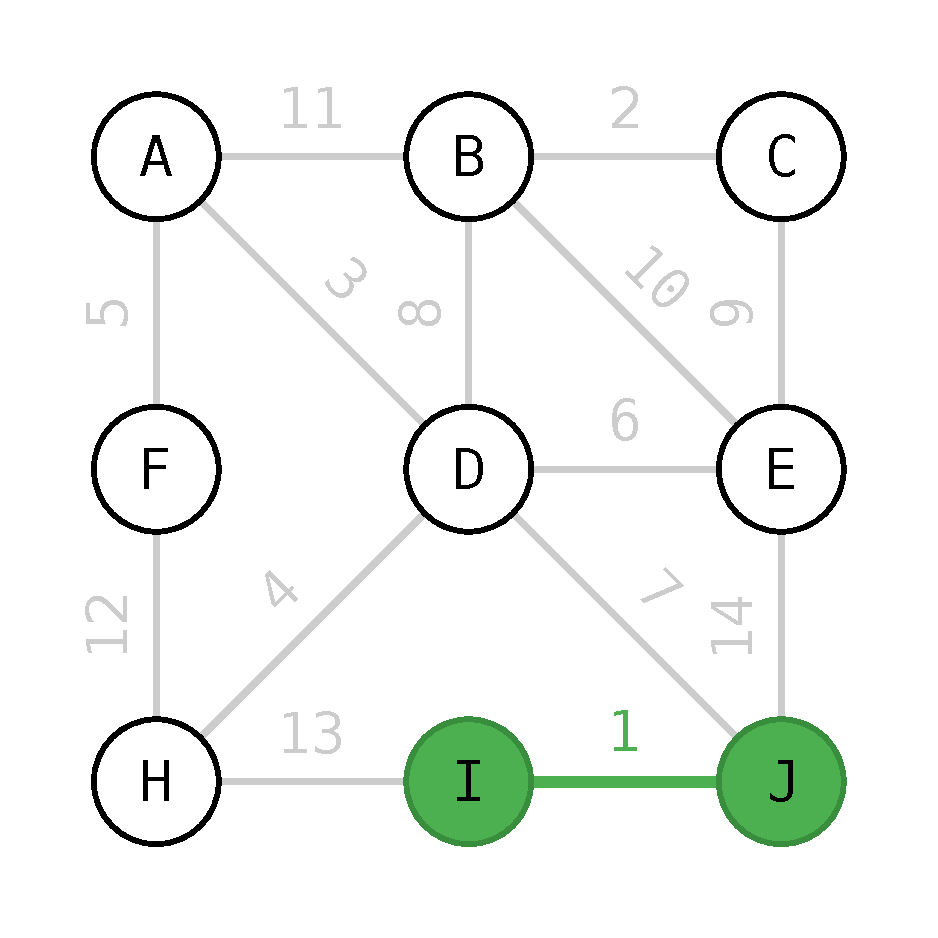
\includegraphics[width=0.30\textwidth]{python/lec08/kruskal/kruskal-1.pdf}\\[2pt]{\scriptsize Шаг 1. $+JI(1)$}} &
\shortstack{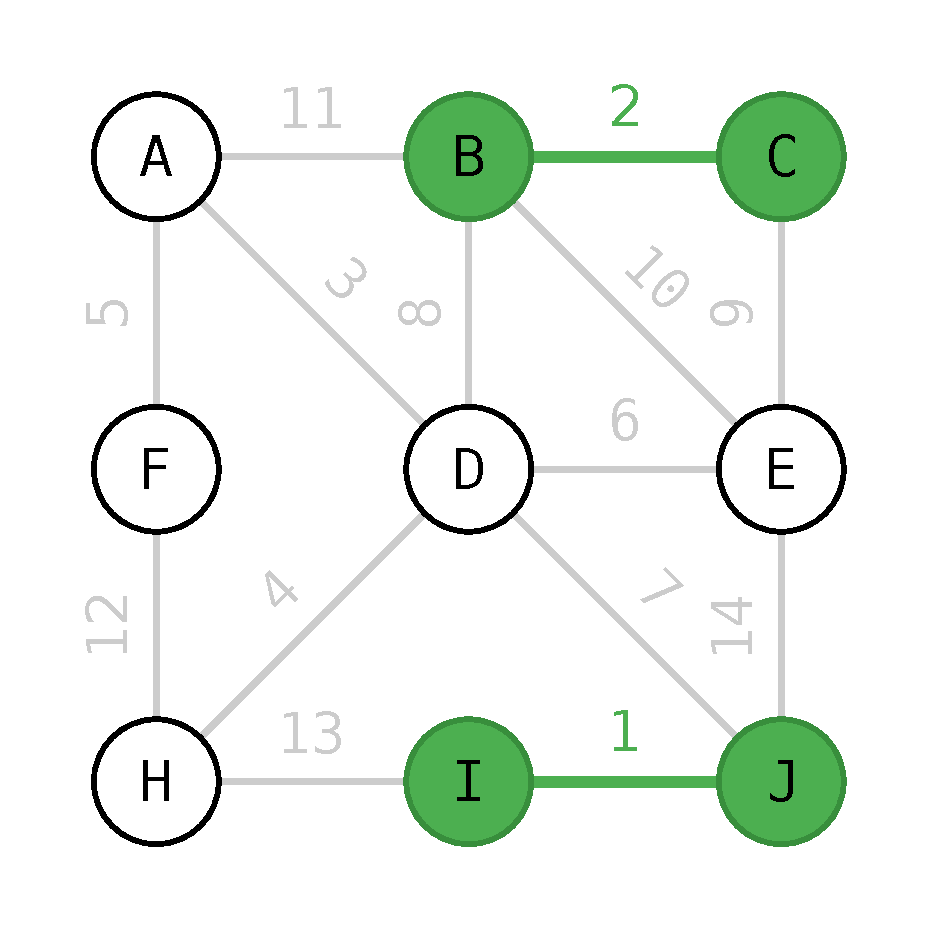
\includegraphics[width=0.30\textwidth]{python/lec08/kruskal/kruskal-2.pdf}\\[2pt]{\scriptsize Шаг 2. $+BC(2)$}} \\
\end{tabular}\end{center}
\begin{center}\begin{tabular}{ccc}
\shortstack{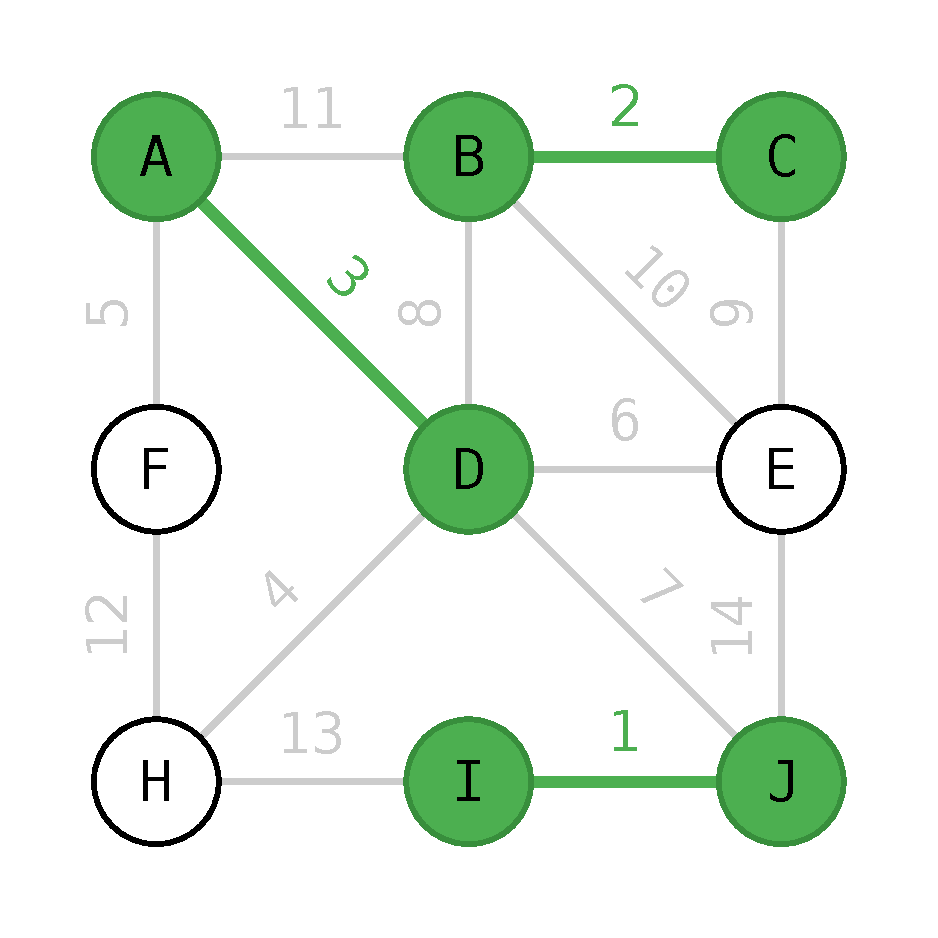
\includegraphics[width=0.30\textwidth]{python/lec08/kruskal/kruskal-3.pdf}\\[2pt]{\scriptsize Шаг 3. $+AD(3)$}} &
\shortstack{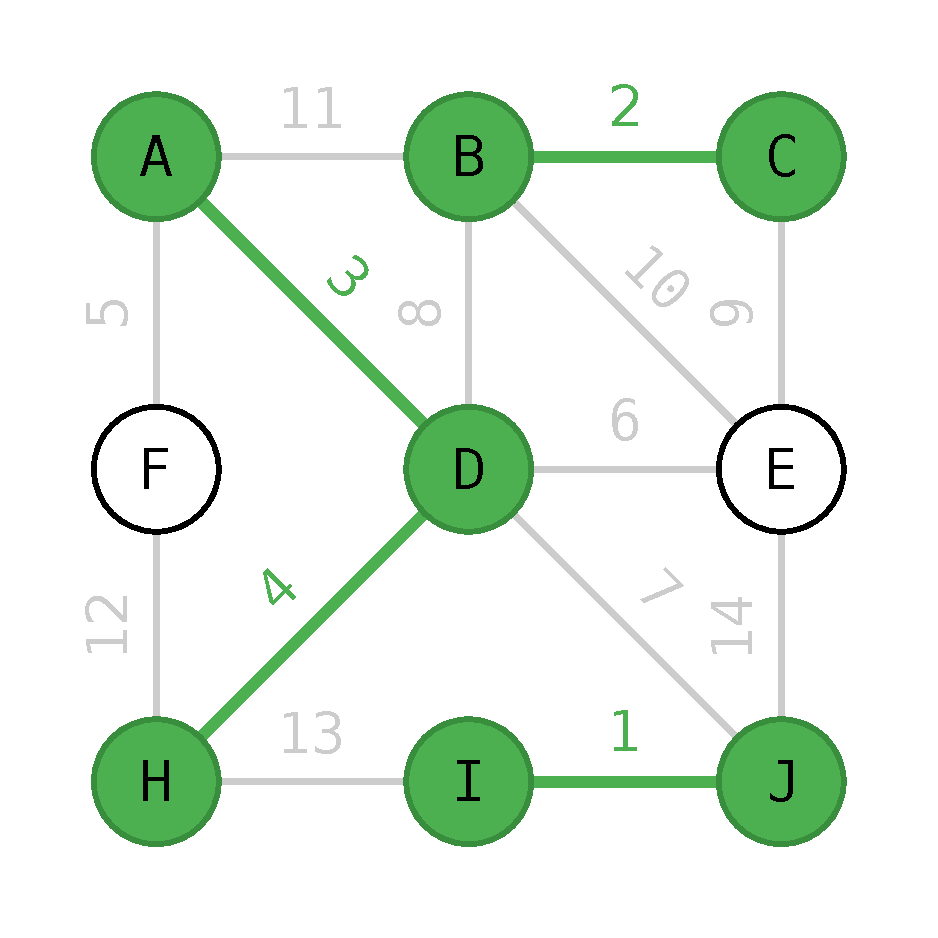
\includegraphics[width=0.30\textwidth]{python/lec08/kruskal/kruskal-4.pdf}\\[2pt]{\scriptsize Шаг 4. $+HD(4)$}} &
\shortstack{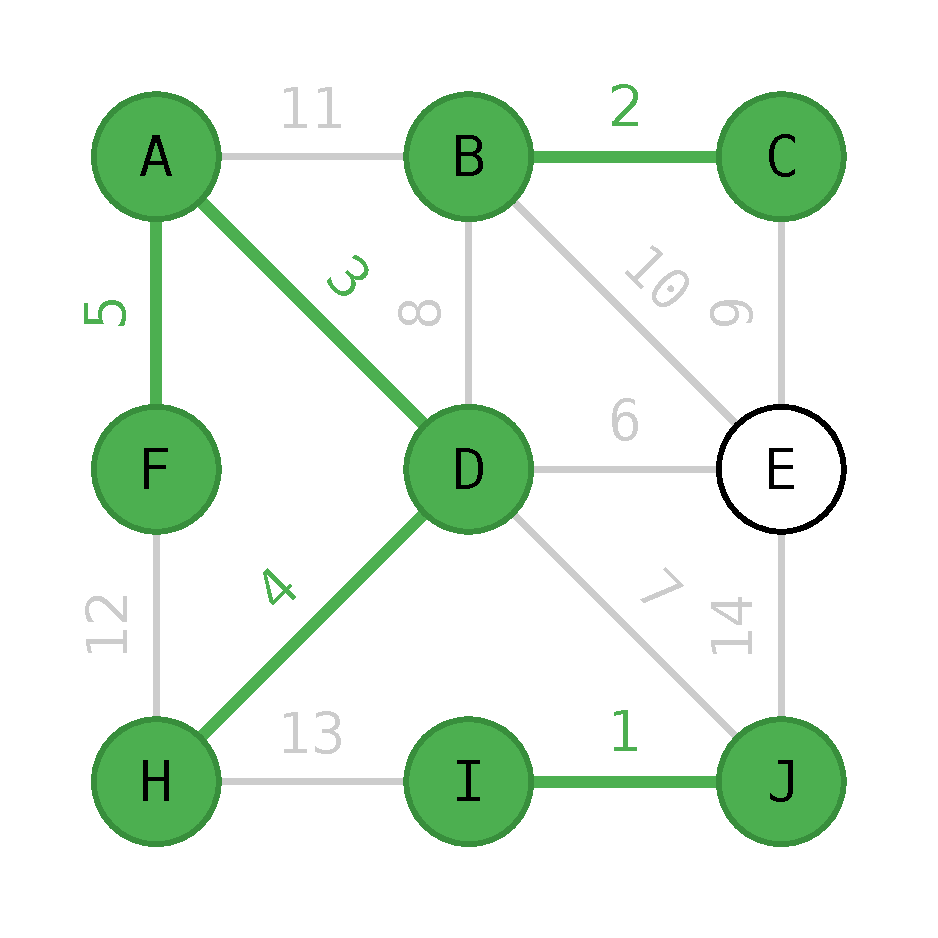
\includegraphics[width=0.30\textwidth]{python/lec08/kruskal/kruskal-5.pdf}\\[2pt]{\scriptsize Шаг 5. $+AF(5)$}} \\
\end{tabular}\end{center}
\begin{center}\begin{tabular}{ccc}
\shortstack{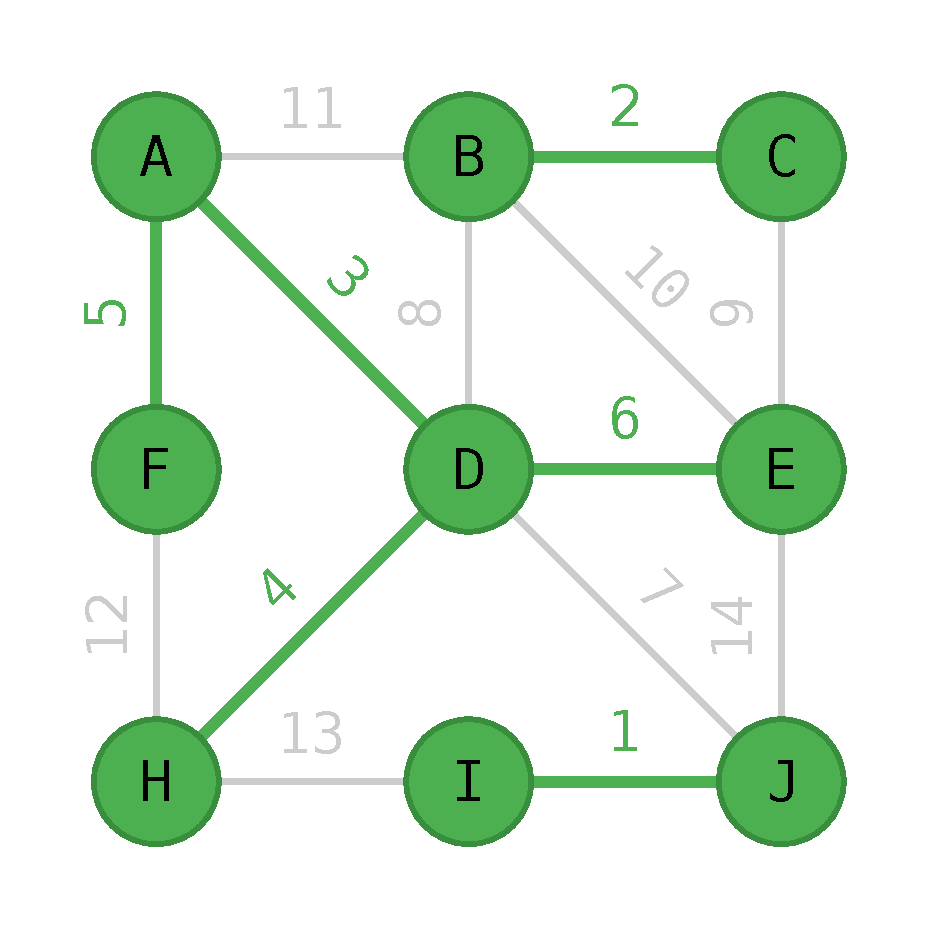
\includegraphics[width=0.30\textwidth]{python/lec08/kruskal/kruskal-6.pdf}\\[2pt]{\scriptsize Шаг 6. $+DE(6)$}} &
\shortstack{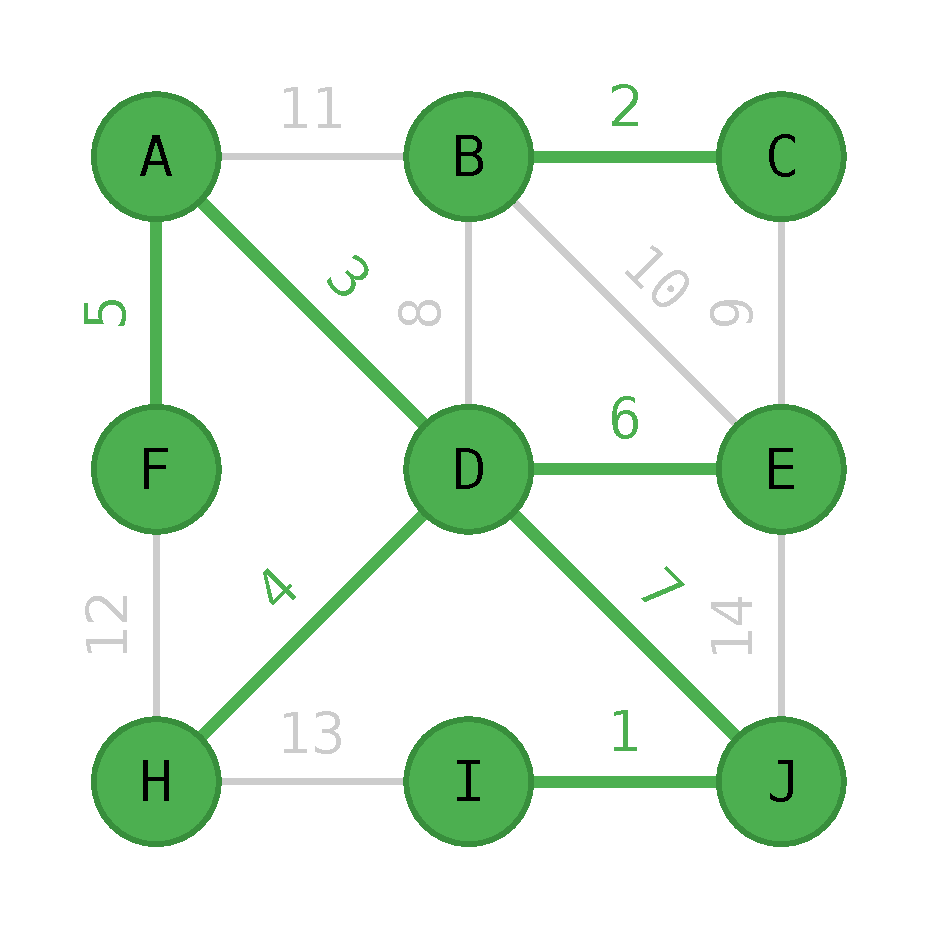
\includegraphics[width=0.30\textwidth]{python/lec08/kruskal/kruskal-7.pdf}\\[2pt]{\scriptsize Шаг 7. $+JD(7)$}} &
\shortstack{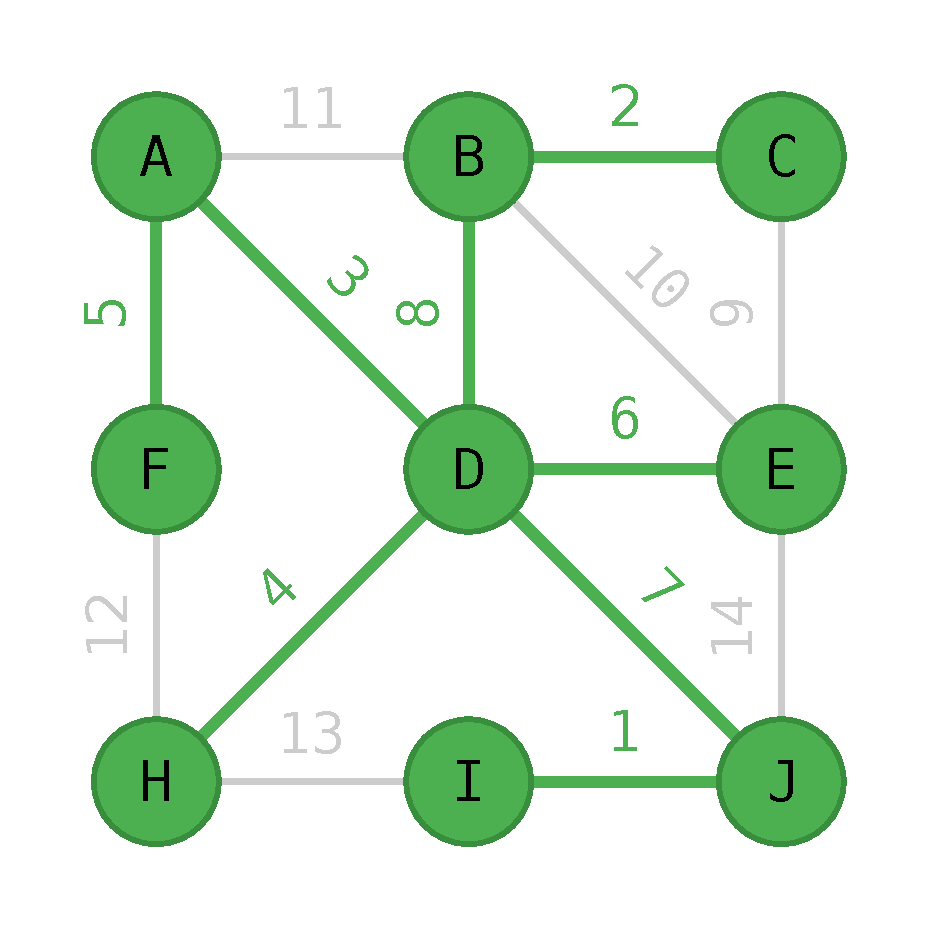
\includegraphics[width=0.30\textwidth]{python/lec08/kruskal/kruskal-8.pdf}\\[2pt]{\scriptsize Шаг 8. $+BD(8)$: остов готов}} \\
\end{tabular}\end{center}
\begin{center}\begin{tabular}{ccc}
\shortstack{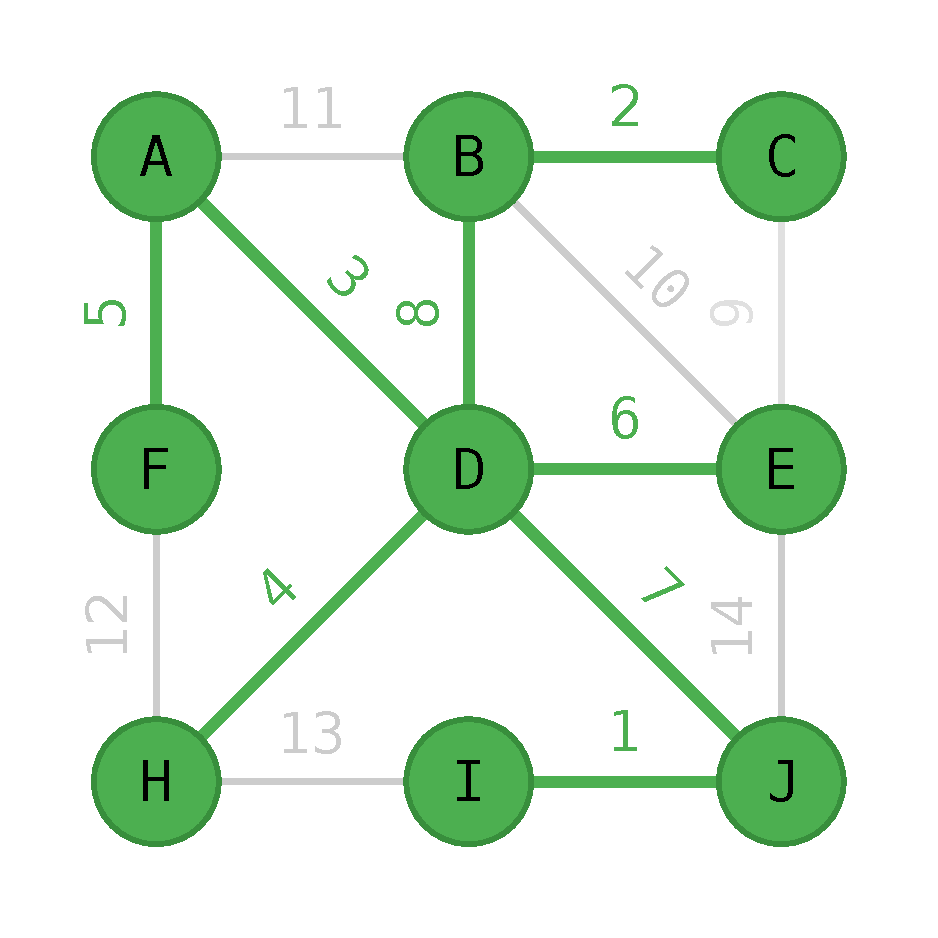
\includegraphics[width=0.30\textwidth]{python/lec08/kruskal/kruskal-9.pdf}\\[2pt]{\scriptsize Шаг 9. $EC(9)$ --- цикл, пропуск}} &
\shortstack{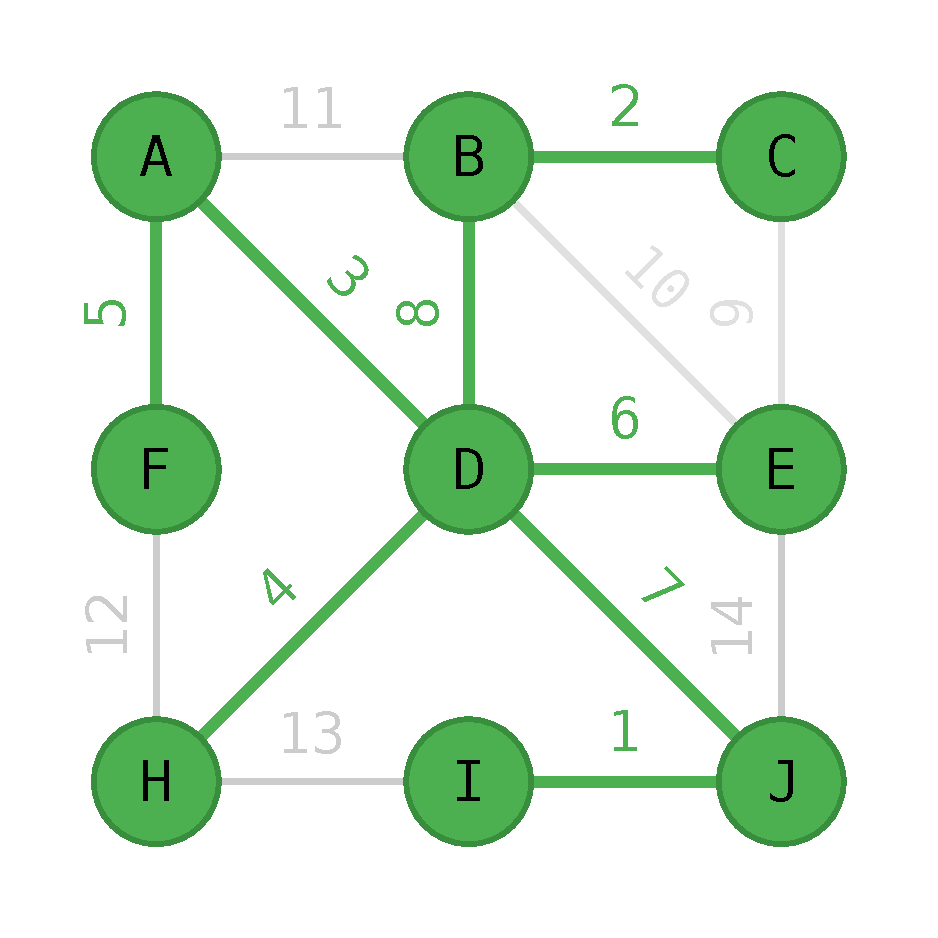
\includegraphics[width=0.30\textwidth]{python/lec08/kruskal/kruskal-10.pdf}\\[2pt]{\scriptsize Шаг 10. $BE(10)$ --- пропуск}} &
\shortstack{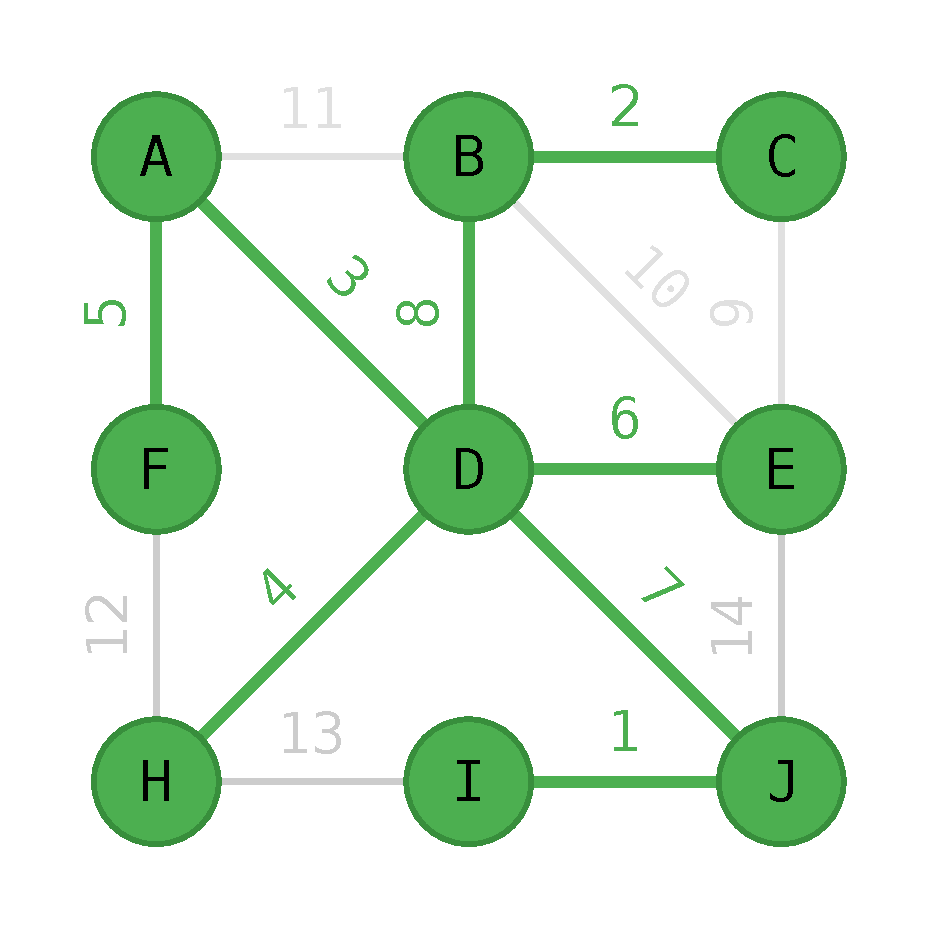
\includegraphics[width=0.30\textwidth]{python/lec08/kruskal/kruskal-11.pdf}\\[2pt]{\scriptsize Шаг 11. $AB(11)$ --- пропуск}} \\
\end{tabular}\end{center}
\begin{center}\begin{tabular}{ccc}
\shortstack{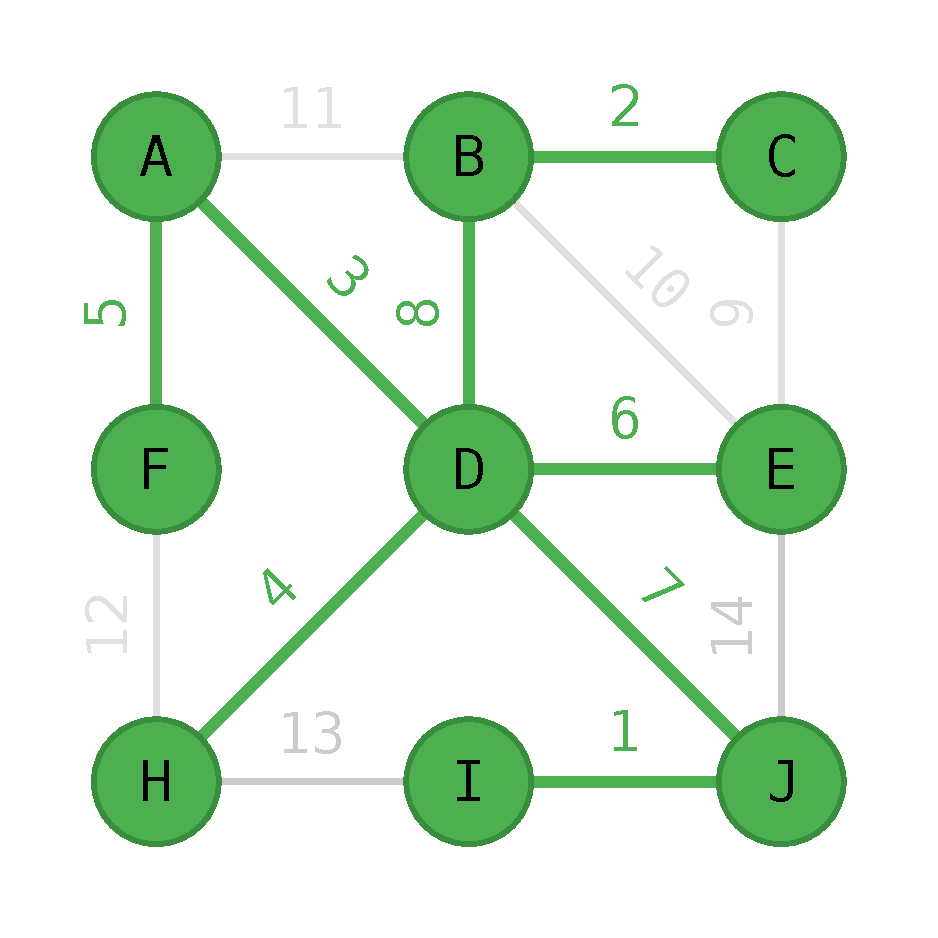
\includegraphics[width=0.30\textwidth]{python/lec08/kruskal/kruskal-12.pdf}\\[2pt]{\scriptsize Шаг 12. $FH(12)$ --- пропуск}} &
\shortstack{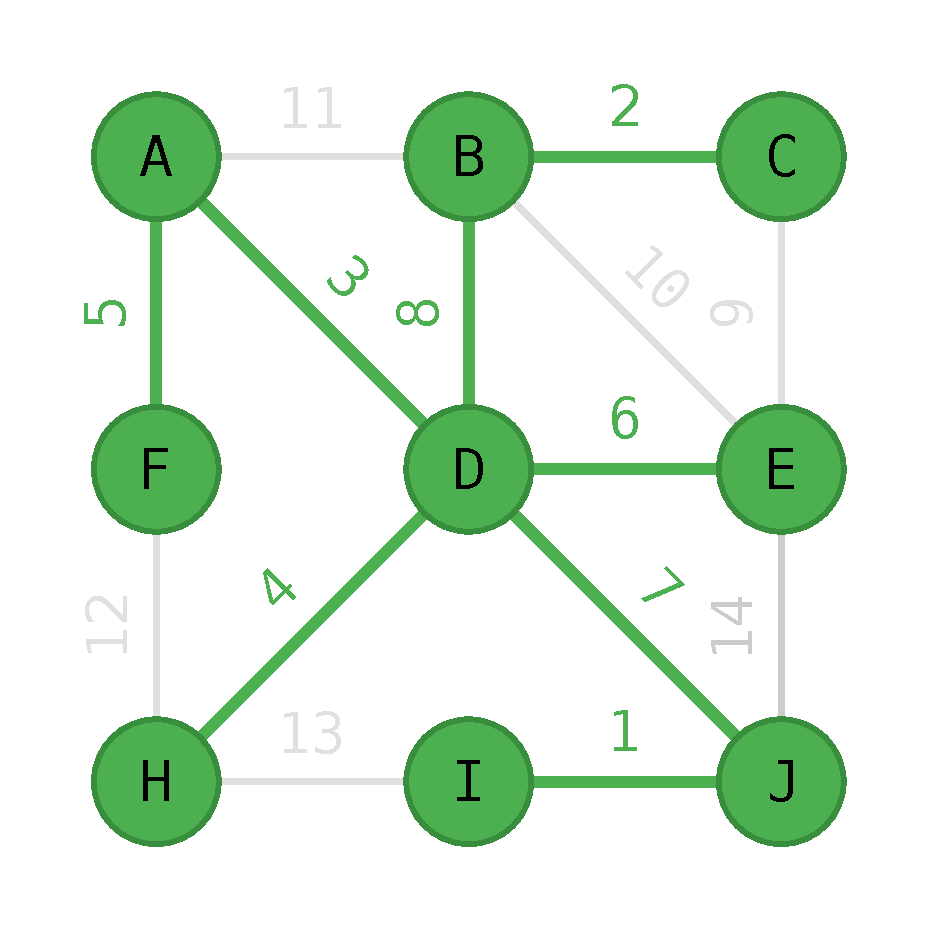
\includegraphics[width=0.30\textwidth]{python/lec08/kruskal/kruskal-13.pdf}\\[2pt]{\scriptsize Шаг 13. $HI(13)$ --- пропуск}} &
\shortstack{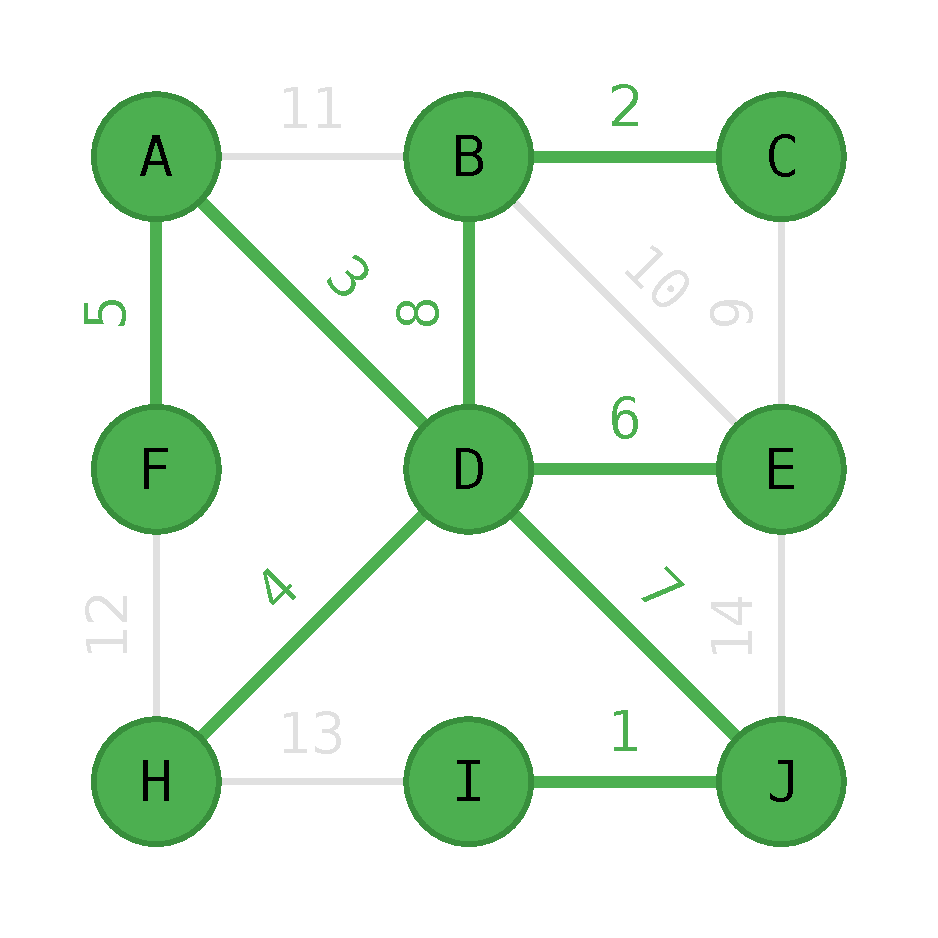
\includegraphics[width=0.30\textwidth]{python/lec08/kruskal/kruskal-14.pdf}\\[2pt]{\scriptsize Шаг 14. $EJ(14)$ --- пропуск}} \\
\end{tabular}\end{center}
\begin{center}
\shortstack{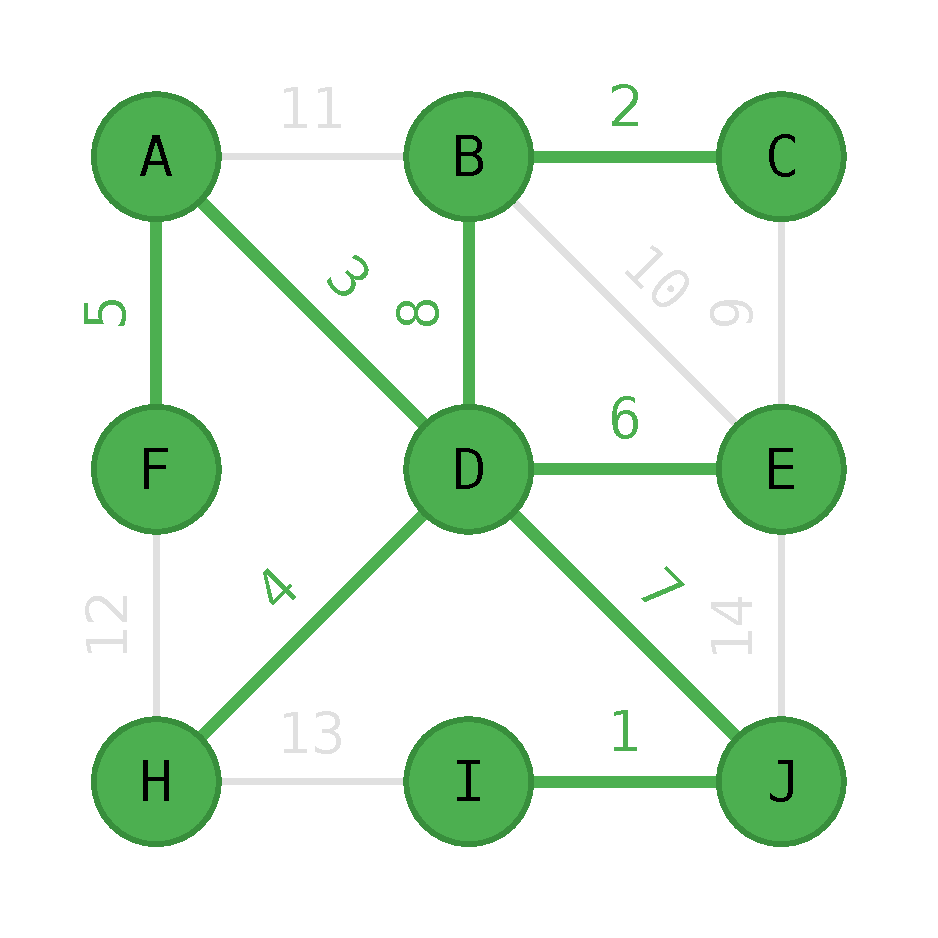
\includegraphics[width=0.32\textwidth]{python/lec08/kruskal/kruskal-15.pdf}\\[2pt]{\scriptsize Шаг 15. Остов построен, $\Sigma = 36$}}
\end{center}
\end{algo}

% ============================================================
% ГЛАВНЫЕ ЦИКЛЫ
% ============================================================

\subsection*{Главные циклы}

\begin{defn}{Хорда}{chord}
$G(V, E)$ --- связный, невзвешенный.

$T_G(V, \hat{E})$ --- остовное дерево $G$.

\textbf{Хорда} $\;\leftrightarrow\;$ $e \in (E \setminus \hat{E})$.
\end{defn}

Зафиксируем в графе остовное дерево; все рёбра вне остова --- хорды:

\begin{center}\begin{tabular}{cc}
\shortstack{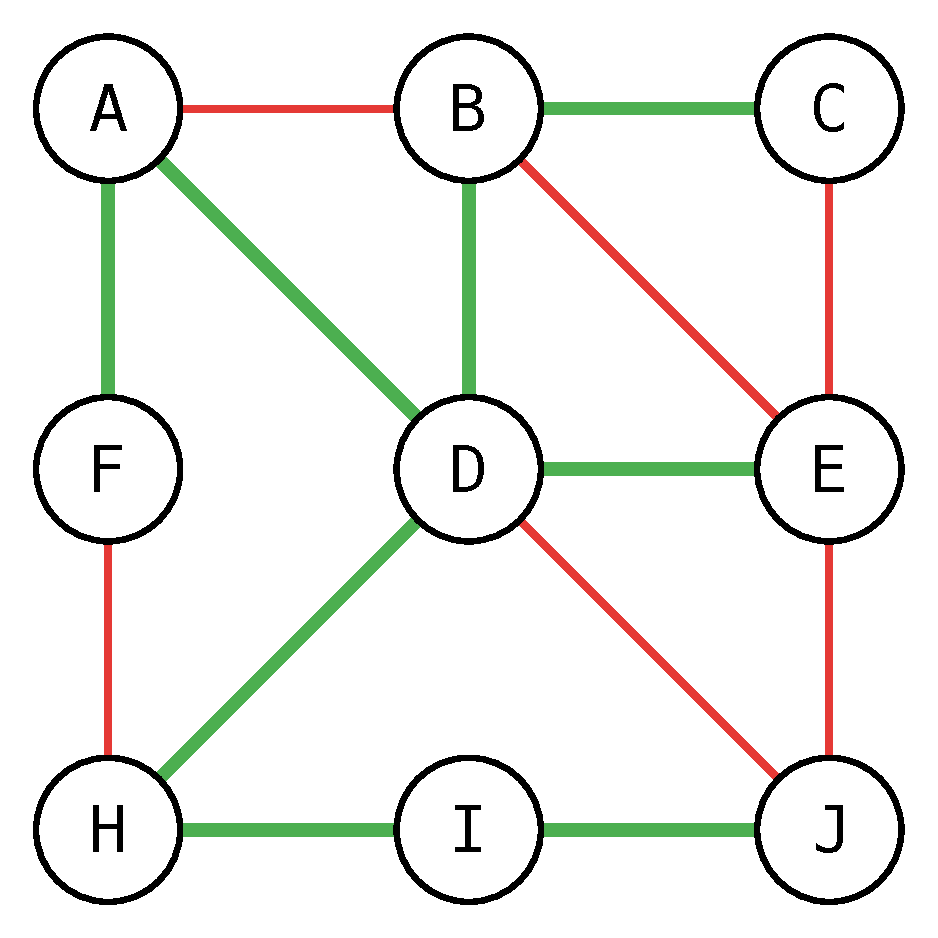
\includegraphics[width=0.42\textwidth]{figures/p20-chords-graph.pdf}\\[2pt]{\scriptsize а) граф $G$: остов --- зелёным, хорды --- красным}} &
\shortstack{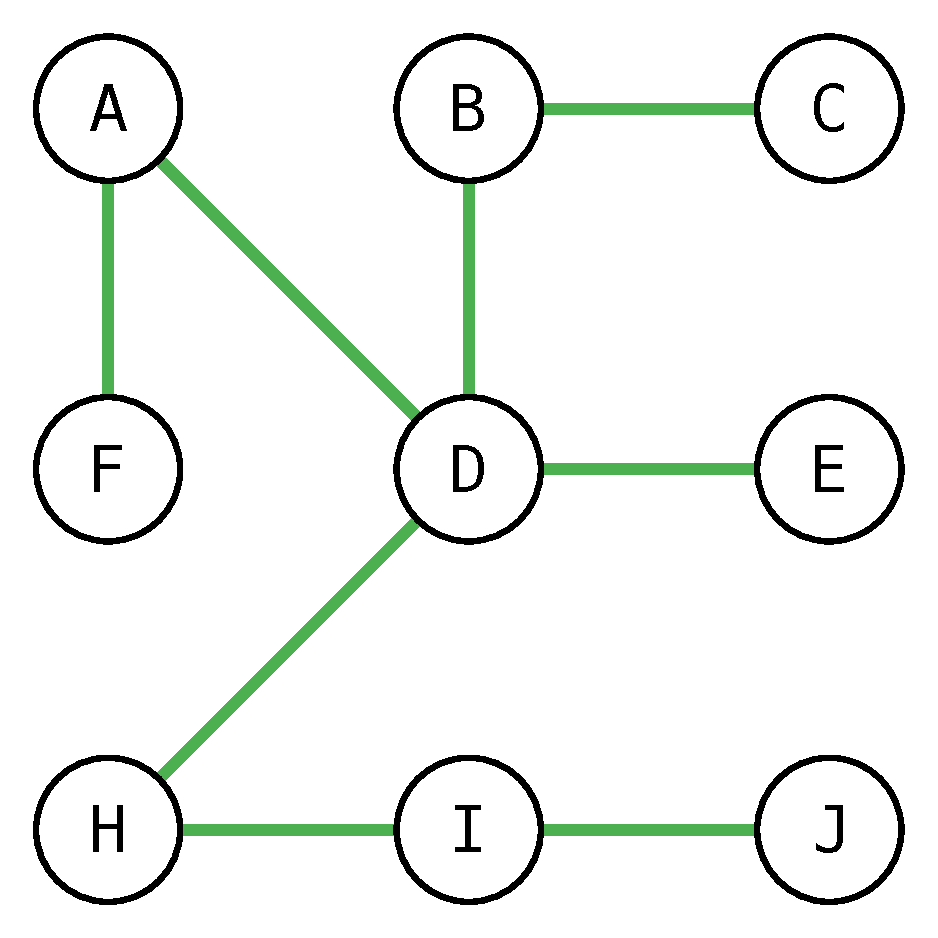
\includegraphics[width=0.42\textwidth]{figures/p20-chords-tree.pdf}\\[2pt]{\scriptsize б) остовное дерево $T_G(V, \hat{E})$ отдельно}} \\
\end{tabular}\end{center}
\grcap{Главные циклы: граф с хордами и его остов}

$G(V, E)$:
$T_G(V, \hat{E})$,\quad $E \setminus \hat{E} = \{e_1, \ldots, e_s\}$ --- набор хорд.

Добавление к дереву любой хорды $e_i$ создаёт ровно один цикл:
$\forall\, 1 \leq i \leq s$:\; $T_G(V, \hat{E}) \cup \{e_i\}$ содержит
цикл $\mathcal{E}_i$ --- \textbf{главный} (хорда $e_i$ плюс единственная
цепь в дереве между её концами).

$\mathcal{E}_1, \ldots, \mathcal{E}_s$ --- набор из $s$ главных циклов.

\medskip
\noindent\textbf{Пример.} Остов
$\hat{E} = \{BC, AD, BD, AF, DH, HI, IJ, DE\}$ (зелёные рёбра на
рисунке), хорды
$E \setminus \hat{E} = \{AB, DJ, BE, FH, EJ, CE\}$ (красные), $s = 6$.
Для каждой хорды выписываем цепь в дереве между её концами и замыкаем:

\begin{enumerate}
  \item $e_1 = AB$: цепь в дереве $A$--$D$--$B$ $\;\Rightarrow\; \mathcal{E}_1 = ABDA$
  \item $e_2 = DJ$: цепь $D$--$H$--$I$--$J$ $\;\Rightarrow\; \mathcal{E}_2 = DHIJD$
  \item $e_3 = BE$: цепь $B$--$D$--$E$ $\;\Rightarrow\; \mathcal{E}_3 = DBED$
  \item $e_4 = FH$: цепь $F$--$A$--$D$--$H$ $\;\Rightarrow\; \mathcal{E}_4 = DAFHD$
  \item $e_5 = EJ$: цепь $E$--$D$--$H$--$I$--$J$ $\;\Rightarrow\; \mathcal{E}_5 = DHIJED$
  \item $e_6 = CE$: цепь $C$--$B$--$D$--$E$ $\;\Rightarrow\; \mathcal{E}_6 = CBDEC$
\end{enumerate}

% ============================================================
% ЦИКЛОВОЕ ПРОСТРАНСТВО
% ============================================================

\subsection*{Цикловое пространство}

\begin{defn}{Сумма циклов}{cycle-sum}
$G(V, E)$,\; $l_1, l_2$ --- 2 цикла (замкнутых пути) в графе.

$l_1 \oplus l_2 := (e \in l_1) \;\Delta\; (e \in l_2)$

\quad (симметрическая разность рёбер).
\end{defn}

$A \,\Delta\, B = (A \cup B) \setminus (B \cap A) = 
\{a \in A \;\&\; a \notin B\} \cup \{a \notin A \;\&\; a \in B\}$:
общие рёбра <<сокращаются>>, остальные остаются.

\medskip
\noindent\textbf{Пример 1.} $\mathcal{E}_1 = ABDA$ (рёбра $AB, BD, DA$),
$\mathcal{E}_6 = CBDEC$ (рёбра $CB, BD, DE, EC$). Общее ребро $BD$
сокращается:
\[
  \mathcal{E}_1 \oplus \mathcal{E}_6
  = \{AB,\; DA,\; CB,\; DE,\; EC\}
  = ABCEDA
\]
--- снова цикл ($A$--$B$--$C$--$E$--$D$--$A$).

\medskip
\noindent\textbf{Пример 2.} $\mathcal{E}_5 = DHIJED$ (рёбра
$DH, HI, IJ, JE, ED$), $\mathcal{E}_4 = DAFHD$ (рёбра $DA, AF, FH, HD$).
Общее ребро $DH$ сокращается:
\[
  \mathcal{E}_5 \oplus \mathcal{E}_4
  = \{HI,\; IJ,\; JE,\; ED,\; DA,\; AF,\; FH\}
  = ADEJIHFA
\]
--- цикл $A$--$D$--$E$--$J$--$I$--$H$--$F$--$A$.

\medskip
\noindent\textbf{Пример 3.} Сложим все четыре:
\[
  l = \mathcal{E}_1 \oplus \mathcal{E}_6 \oplus \mathcal{E}_5 \oplus \mathcal{E}_4
  = (\mathcal{E}_1 \oplus \mathcal{E}_6) \oplus (\mathcal{E}_5 \oplus \mathcal{E}_4).
\]
У циклов $ABCEDA$ и $ADEJIHFA$ общие рёбра $AD$ и $DE$ сокращаются:
\[
  l = \{AB,\; BC,\; CE,\; EJ,\; JI,\; IH,\; HF,\; FA\} = ABCEJIHFA
\]
--- цикл по <<внешнему контуру>> графа, составленный из главных циклов
$\mathcal{E}_1, \mathcal{E}_6, \mathcal{E}_5, \mathcal{E}_4$.

\medskip
\textbf{Замечание.}
\begin{enumerate}[label=\alph*)]
  \item Множество всех <<обобщённых циклов>> (рёберно-непересекающихся
        объединений циклов, включая пустое множество рёбер) с операцией
        $\oplus$ образует векторное пространство над полем $\mathbb{F}_2$
        --- \textbf{цикловое пространство} графа;
  \item главные циклы $\mathcal{E}_1, \ldots, \mathcal{E}_s$ --- базис
        этого пространства: они линейно независимы (каждый содержит
        <<свою>> хорду, которой нет в остальных), и любой цикл $l$
        раскладывается по ним --- $l$ есть сумма главных циклов тех
        хорд, которые входят в $l$;
  \item размерность циклового пространства равна числу хорд:
        $s = |E| - |\hat E| = |E| - (|V| - 1) = |E| - |V| + 1$
        (\emph{цикломатическое число} графа). В примере выше:
        $s = 14 - 9 + 1 = 6$.
\end{enumerate}

\medskip
\textbf{Упр.} $G(V, E)$ --- связный, fix $T_G(V, \hat{E})$,
$\mathcal{E}_1, \ldots, \mathcal{E}_s$ --- главные циклы. Доказать
аккуратно пункты a) и b) замечания: что $(\{\text{обобщённые циклы}\},
\oplus)$ --- векторное пространство над $\mathbb{F}_2$ и что
$\mathcal{E}_1, \ldots, \mathcal{E}_s$ --- его базис.

% ============================================================
\begin{task}{Минимальное остовное дерево: алгоритм Краскала}{kruskal-task}
\textbf{Условие.} Дан неориентированный взвешенный граф на вершинах
$A,B,C,D,E,F,G$ с рёбрами
\begin{gather*}
  AB=7,\quad AD=5,\quad BC=8,\quad BD=9,\quad BE=7,\quad CE=5,\\
  DE=15,\quad DF=6,\quad EF=8,\quad EG=9,\quad FG=11.
\end{gather*}
Постройте минимальное остовное дерево алгоритмом Краскала. Укажите
порядок включения рёбер и суммарный вес.

\begin{center}
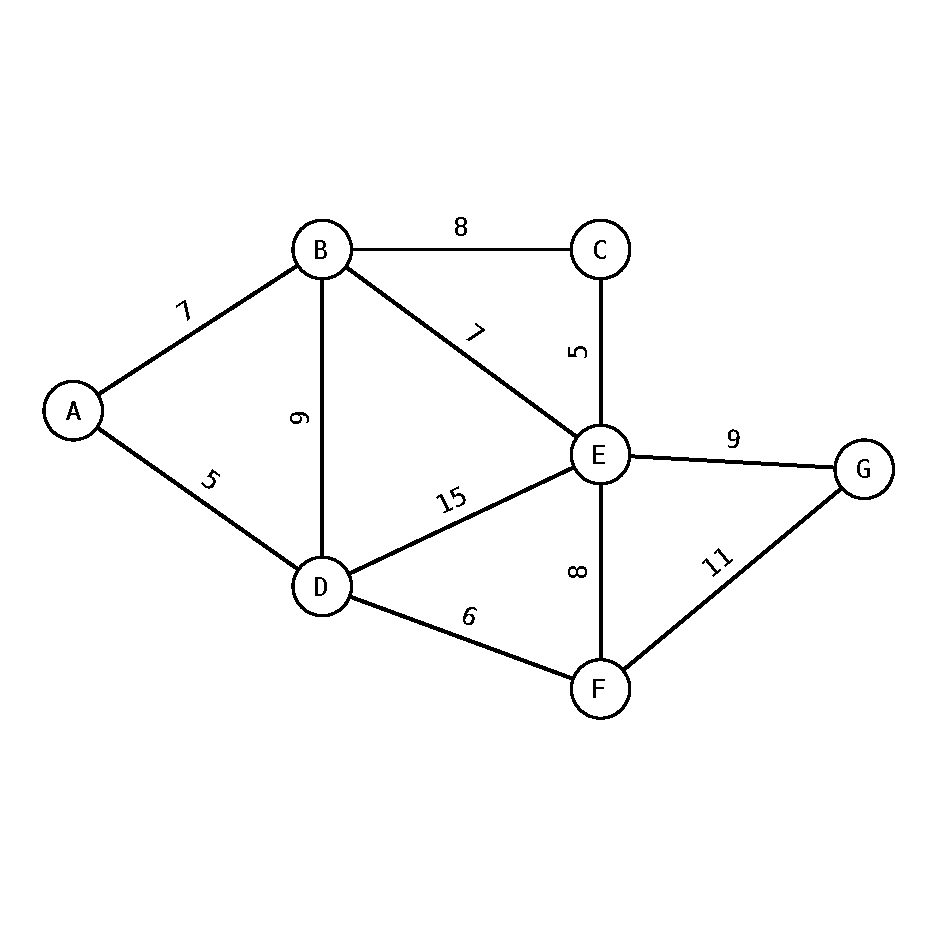
\includegraphics[width=0.5\textwidth]{figures/task-kruskal-1.pdf}
\end{center}

\textbf{Решение.} Краскал сортирует рёбра по возрастанию веса и добавляет ребро,
если его концы лежат в разных компонентах (что отслеживается системой
непересекающихся множеств) --- иначе ребро замкнуло бы цикл.

Отсортированный список рёбер:
\[
  AD(5),\ CE(5),\ DF(6),\ AB(7),\ BE(7),\ BC(8),\ EF(8),\ BD(9),\ EG(9),\ FG(11),\ DE(15).
\]
\begin{enumerate}
  \item $AD(5)$ --- компоненты $\{A\},\{D\}$ различны, добавляем $\Rightarrow\{A,D\}$.
  \item $CE(5)$ --- добавляем $\Rightarrow\{C,E\}$.
  \item $DF(6)$ --- $F$ присоединяется к $\{A,D\}$, добавляем $\Rightarrow\{A,D,F\}$.
  \item $AB(7)$ --- $B$ присоединяется, добавляем $\Rightarrow\{A,B,D,F\}$.
  \item $BE(7)$ --- сливаем $\{A,B,D,F\}$ и $\{C,E\}$, добавляем
        $\Rightarrow\{A,B,C,D,E,F\}$.
  \item $BC(8)$ --- $B$ и $C$ уже в одной компоненте: \emph{цикл, пропускаем}.
  \item $EF(8)$ --- цикл, пропускаем.
  \item $BD(9)$ --- цикл, пропускаем.
  \item $EG(9)$ --- $G$ присоединяется, добавляем. Все $7$ вершин в одной
        компоненте, набрано $6 = 7 - 1$ рёбер --- остов построен.
  \item $FG(11),\ DE(15)$ --- цикл, пропускаем.
\end{enumerate}

\medskip
\noindent Ключевые шаги построения:

\begin{center}\begin{tabular}{ccc}
\shortstack{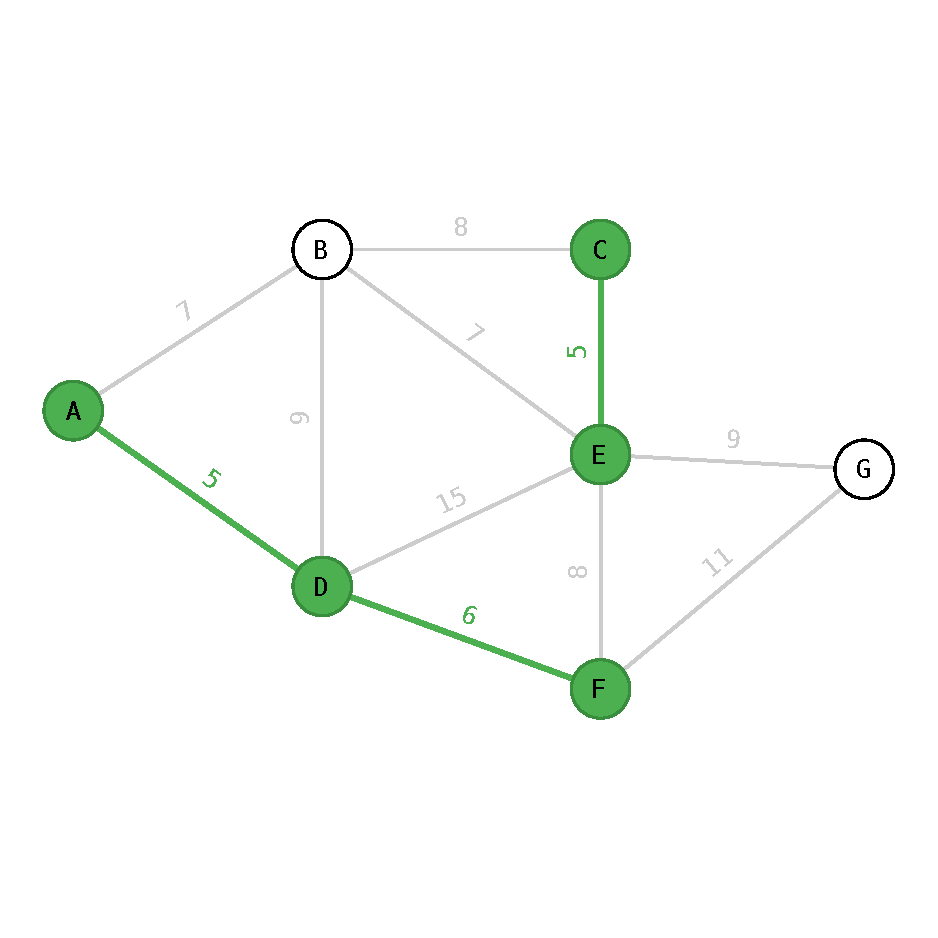
\includegraphics[width=0.30\textwidth]{python/lec08/kruskal_task/kruskalt-3.pdf}\\[2pt]{\scriptsize $+AD, +CE, +DF$}} &
\shortstack{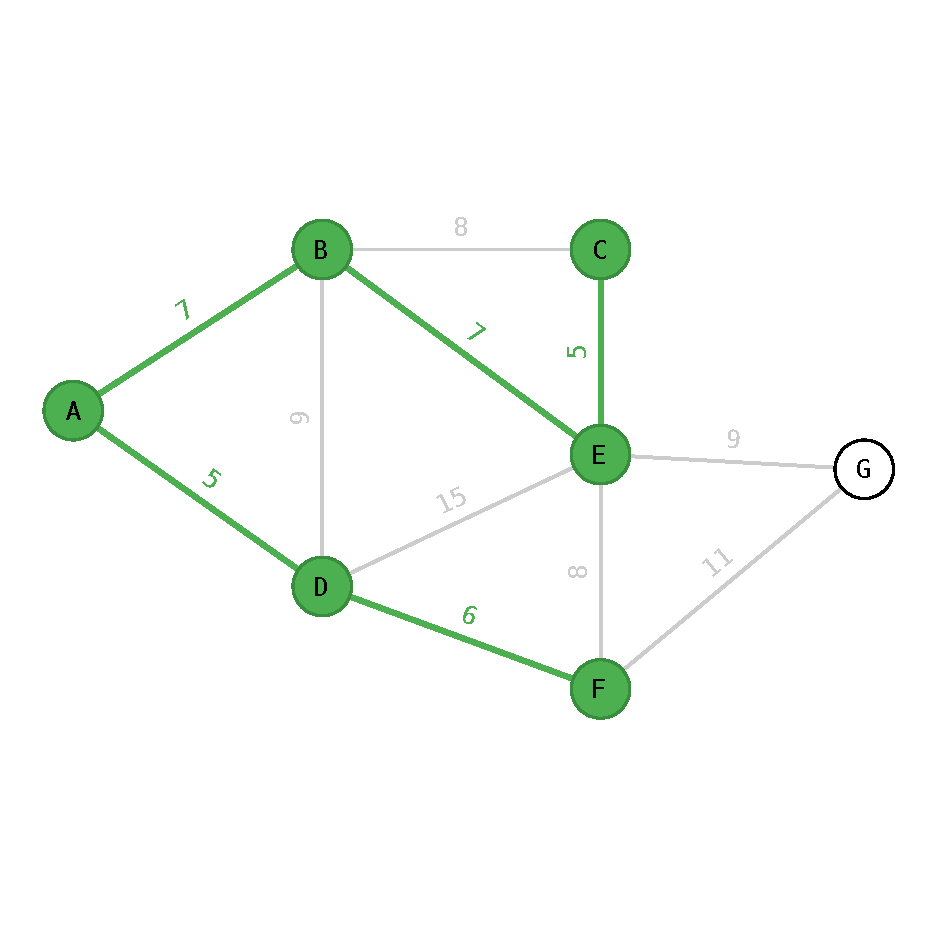
\includegraphics[width=0.30\textwidth]{python/lec08/kruskal_task/kruskalt-5.pdf}\\[2pt]{\scriptsize $+AB, +BE$}} &
\shortstack{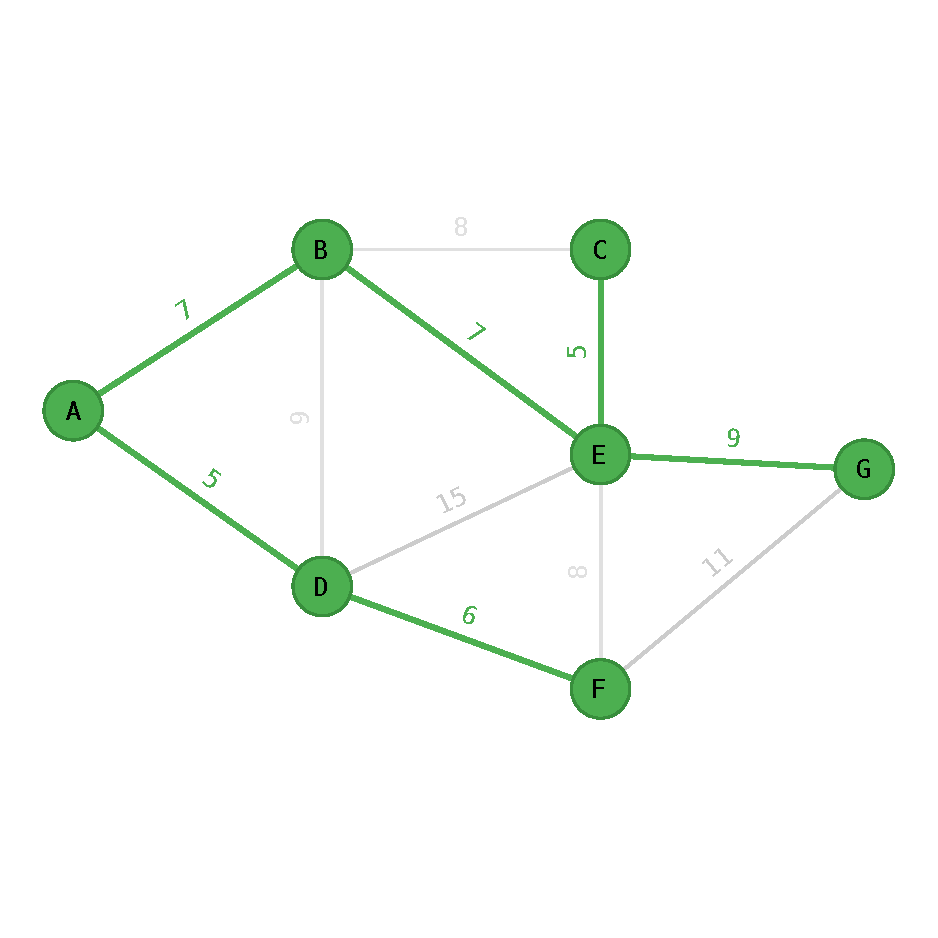
\includegraphics[width=0.30\textwidth]{python/lec08/kruskal_task/kruskalt-9.pdf}\\[2pt]{\scriptsize пропуски $BC, EF, BD$; $+EG$}} \\
\end{tabular}\end{center}
\begin{center}
\shortstack{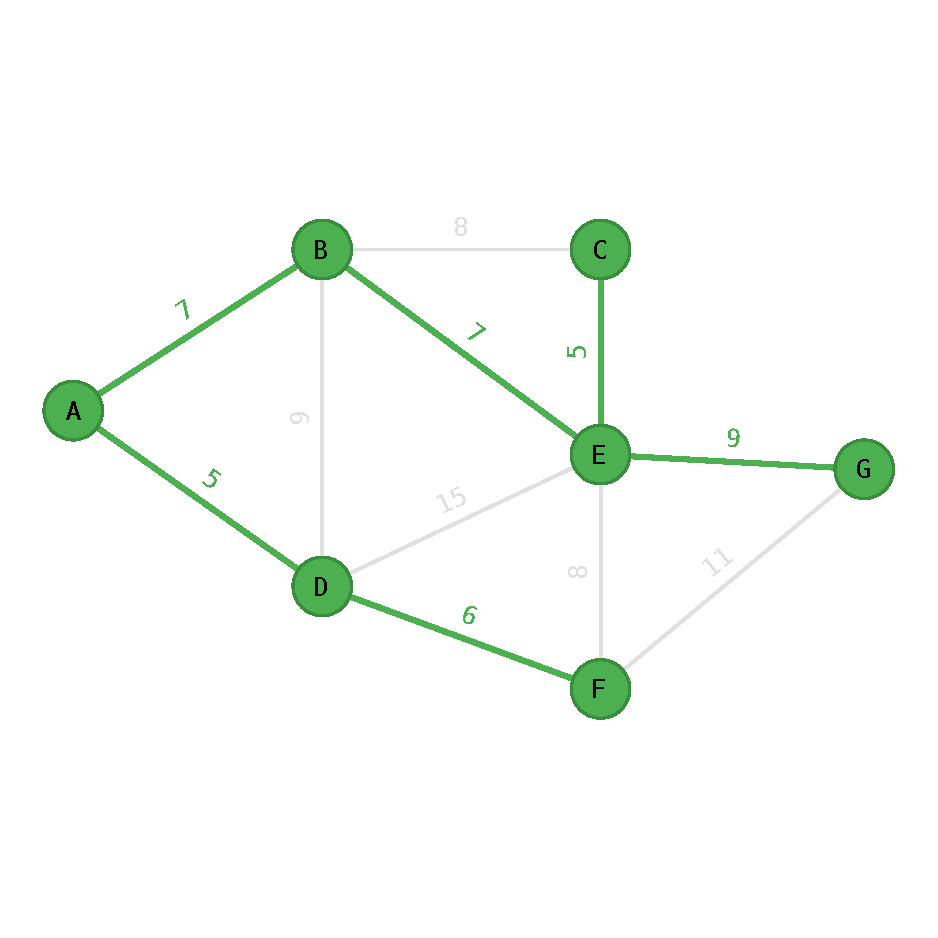
\includegraphics[width=0.34\textwidth]{python/lec08/kruskal_task/kruskalt-12.pdf}\\[2pt]{\scriptsize Остов построен, $\Sigma = 39$}}
\end{center}

\textbf{Ответ.} Остовное дерево: рёбра $AD,CE,DF,AB,BE,EG$; суммарный вес
$5+5+6+7+7+9=39$.
\end{task}


\chapter{Лекция 9. Двудольные графы. Паросочетания. Задача о максимальном потоке}

% ============================================================
% ДВУДОЛЬНЫЕ ГРАФЫ
% ============================================================

\subsection*{Двудольные графы}

\begin{defn}{Двудольный граф}{bipartite}
$G(V, E)$ --- \textbf{двудольный}:

$V = V_1 \sqcup V_2$ т.\,ч. $\forall\, e \in E$: $u \in V_1$, $v \in V_2$
\quad (начальная вершина --- любая).
\end{defn}

\medskip
\noindent\textbf{Примеры} (доля $V_1$ --- синяя, доля $V_2$ --- оранжевая):

% Пример 1: дерево (11 вершин) — двудольный
% Граф: p21-example-1.graph
\grfig{figures/p21-example-1.pdf}{Двудольный: дерево 11 вершин}
\noindent\textit{Пример 1.} Любое дерево двудольно: раскрашиваем вершины
по чётности уровня. Здесь $V_1 = \{1, 3, 4, 6, 9, 11\}$ (чётные уровни),
$V_2 = \{2, 5, 7, 8, 10\}$ (нечётные) --- каждое ребро соединяет
соседние уровни, т.\,е. разные доли.

% Пример 2: решётка/сетка (10 вершин) — двудольный
% Граф: p21-example-2.graph
\grfig{figures/p21-example-2.pdf}{Двудольный: решётка 10 вершин}
\noindent\textit{Пример 2.} Решётка двудольна (<<шахматная>> раскраска):
$V_1 = \{1, 3, 6, 8, 9\}$, $V_2 = \{2, 4, 5, 7, 10\}$ --- у каждого
ребра концы разного цвета.

% Пример 3: треугольник (3 вершины) — НЕ двудольный
% Граф: p21-example-3.graph
\grfig{figures/p21-example-3.pdf}{НЕ двудольный: треугольник}
\noindent\textit{Пример 3.} Треугольник \emph{не} двудолен: положив
$1 \in V_1$, получаем $2 \in V_2$, $3 \in V_1$ --- но тогда ребро
$3$--$1$ (красное) соединяет две вершины одной доли. Куда ни относи
вершины, одно ребро всегда останется внутри доли.

\begin{statement}{Критерий двудольности графа}{bipartite-criterion}
$G$ --- двудольный $\;\Leftrightarrow\;$ $G$ не содержит циклов нечётной длины.
\end{statement}

\begin{proof}
\textbf{($\Rightarrow$) Если граф двудолен, нечётных циклов нет.} Пусть
$V=V_1\sqcup V_2$ --- доли, и все рёбра идут между ними. Любой цикл
$v_0\,v_1\,\dots\,v_k\,v_0$ при движении по рёбрам поочерёдно меняет долю:
$v_0\in V_1\Rightarrow v_1\in V_2\Rightarrow v_2\in V_1$ и так далее. Чтобы
вернуться в исходную долю (в вершину $v_0$), число шагов должно быть чётным,
поэтому длина любого цикла чётна --- нечётных циклов нет.

\smallskip
\textbf{($\Leftarrow$) Если нечётных циклов нет, граф двудолен.} Достаточно
доказать утверждение для каждой связной компоненты по отдельности. Зафиксируем
в компоненте вершину $s$ и для каждой вершины $v$ рассмотрим расстояние
$d(s,v)$ (длину кратчайшего пути, BFS-нумерация). Положим
\[
  V_1=\{v\colon d(s,v)\text{ чётно}\},\qquad
  V_2=\{v\colon d(s,v)\text{ нечётно}\}.
\]
Покажем, что любое ребро $uv$ соединяет вершины из разных долей. Предположим
противное: пусть $u,v$ лежат в одной доле, то есть $d(s,u)$ и $d(s,v)$ одной
чётности. Рассмотрим замкнутый маршрут: кратчайший путь $s\to u$, ребро $uv$ и
кратчайший путь $v\to s$. Его длина равна $d(s,u)+1+d(s,v)$ --- сумма двух
чисел одной чётности плюс единица, то есть \emph{нечётна}. Замкнутый маршрут
нечётной длины обязательно содержит простой цикл нечётной длины, что
противоречит условию. Значит концы каждого ребра попадают в разные доли, и
разбиение $V=V_1\sqcup V_2$ задаёт двудольность.

\smallskip
\textit{Иллюстрация.} Цикл \emph{чётной} длины ($C_8$ слева)
раскрашивается чередованием $V_1,V_2,V_1,V_2,\dots$ --- двудолен. В цикле
\emph{нечётной} длины ($C_7$ справа) при таком чередовании последняя
вершина оказывается смежной с первой вершиной той же доли (красное
ребро) --- разбить на две доли невозможно.

\grfig[0.45]{figures/p21-example-4.pdf}{Критерий: чётный цикл $C_8$ (двудольный)}
\grfig[0.45]{figures/p21-example-5.pdf}{Критерий: нечётный цикл $C_7$ (не двудольный)}

\end{proof}

% ============================================================
% ПАРОСОЧЕТАНИЯ
% ============================================================

\subsection*{Паросочетания}

\begin{defn}{Паросочетание}{matching}
$G(V, E)$ --- двудольный, $V = V_1 \sqcup V_2$.

\textbf{Паросочетание} для $G$: $\hat{E} \subseteq E$ т.\,ч. $\forall\, e_i, e_j \in \hat{E}$
--- инцидентны не более чем одной общей вершине
(т.\,е. рёбра паросочетания попарно не имеют общих вершин).
\end{defn}

\begin{defn}{Максимальное паросочетание}{max-matching}
\textbf{Максимальное паросочетание} --- максимальное по включению:
к нему нельзя добавить ни одно ребро графа, не нарушив определение.
\end{defn}

\begin{defn}{Наибольшее паросочетание}{maximum-matching}
\textbf{Наибольшее паросочетание} --- наибольшее количество рёбер для данного графа.
\end{defn}

\medskip
\noindent\textbf{Примеры.} Один и тот же граф --- цепь $1$--$2$--$3$--$4$;
рёбра паросочетания --- зелёные жирные, насыщенные ими вершины ---
закрашены:

% Пример 1: {1-2} — не макс, не наиб.
% Граф: p22-example-1.graph
\grfig[0.4]{figures/p22-example-1.pdf}{Паросочетание $\{1\text{--}2\}$: не макс., не наиб.}
\noindent\textit{Пример 1.} $\hat E = \{1\text{--}2\}$ --- \textbf{не
максимальное}: можно добавить ребро $3$--$4$ (его концы свободны);
значит, и \textbf{не наибольшее}.

% Пример 2: {2-3} — макс., не наиб.
% Граф: p22-example-2.graph
\grfig[0.4]{figures/p22-example-2.pdf}{Паросочетание $\{2\text{--}3\}$: макс., но не наиб.}
\noindent\textit{Пример 2.} $\hat E = \{2\text{--}3\}$ ---
\textbf{максимальное}: оба оставшихся ребра ($1$--$2$ и $3$--$4$)
задевают занятые вершины $2$ и $3$, добавить нечего. Но \textbf{не
наибольшее}: в примере~3 есть паросочетание из двух рёбер.

% Пример 3: {1-2, 3-4} — макс. и наиб.
% Граф: p22-example-3.graph
\grfig[0.4]{figures/p22-example-3.pdf}{Паросочетание $\{1\text{--}2,\ 3\text{--}4\}$: макс. и наиб.}
\noindent\textit{Пример 3.} $\hat E = \{1\text{--}2,\ 3\text{--}4\}$ ---
\textbf{максимальное и наибольшее}: все 4 вершины насыщены, больше двух
непересекающихся рёбер в графе из 4 вершин быть не может.

% Пример 4: {3-4} — не макс., не наиб.
% Граф: p22-example-4.graph
\grfig[0.4]{figures/p22-example-4.pdf}{Паросочетание $\{3\text{--}4\}$: не макс., не наиб.}
\noindent\textit{Пример 4.} $\hat E = \{3\text{--}4\}$ --- симметричный
к примеру~1 случай: можно добавить ребро $1$--$2$, поэтому паросочетание
\textbf{не максимальное} (и не наибольшее).

\medskip
\textbf{NB:} $\max |\hat E| \leq \min(|V_1|, |V_2|)$ --- каждое ребро
паросочетания занимает по одной вершине в каждой доле, поэтому рёбер не
больше, чем вершин в меньшей доле.

\medskip
\textbf{Упр.} Доказать, что:
\begin{itemize}
  \item наибольшее $\Rightarrow$ максимальное;
  \item максимальное $\not\Rightarrow$ наибольшее.
\end{itemize}

\textit{Решение.} Если бы наибольшее паросочетание не было максимальным,
к нему можно было бы добавить ребро и получить паросочетание большего
размера --- противоречие с <<наибольшестью>>. Обратная импликация
неверна: контрпример --- примеры 2 и 3 выше ($\{2\text{--}3\}$
максимально, но меньше наибольшего).

\medskip
\textbf{Упр.} Пример $G$ с наибольшим паросочетанием $\hat{E}$, т.\,ч. $|\hat{E}| < \min(|V_1|, |V_2|)$.

\textit{Решение.} <<Звезда>>: $V_1 = \{a, b\}$, $V_2 = \{x, y\}$, рёбра
$a$--$x$, $a$--$y$. Все рёбра проходят через $a$, поэтому любое
паросочетание содержит не более одного ребра: $|\hat E| = 1 <
2 = \min(|V_1|, |V_2|)$.

% ============================================================
% АЛГОРИТМ НАХОЖДЕНИЯ НАИБОЛЬШЕГО ПАРОСОЧЕТАНИЯ
% ============================================================

\begin{algo}{Алгоритм поиска наибольшего паросочетания}{matching-algo}
\textbf{Дано:} $G(V, E)$ --- двудольный, $V = V_1 \sqcup V_2$.

\textbf{Найти:} наибольшее паросочетание $\hat{E}$.

\medskip
\textbf{Инициализация.} Добавляем фиктивные вершины $S$ и $F$:
\[
  \forall\, v_i \in V_1\colon\ \text{дуга } S \to v_i;
  \qquad
  \forall\, w_j \in V_2\colon\ \text{дуга } w_j \to F,
\]
а все рёбра графа ориентируем слева направо: $v_i \to w_j$.

\medskip
\textbf{Step.} Пока существует путь $l\colon S \to \ldots \to F$:
\begin{enumerate}
  \item находим такой путь (любым обходом);
  \item \emph{инвертируем} на нём все рёбра между долями:
        пройденное ребро $v_i \to w_j$ разворачивается в $w_j \to v_i$
        --- развёрнутые рёбра и есть текущее паросочетание;
  \item крайние дуги пути ($S \to v_i$ и $w_j \to F$) удаляем ---
        вершины $v_i$ и $w_j$ насыщены.
\end{enumerate}
Когда путей из $S$ в $F$ больше нет, развёрнутые рёбра $w_j \to v_i$
образуют наибольшее паросочетание.

\medskip
\textit{Почему это работает:} путь $S \to v_i \to w_j \to v_k \to \ldots
\to F$, проходящий по развёрнутому ребру $w_j \to v_k$, --- это
\emph{увеличивающий путь}: он отбирает $w_j$ у вершины $v_k$ и тут же
находит ей новую пару, а в конце насыщает одну новую вершину каждой
доли. Число рёбер паросочетания каждый раз растёт на $1$.

\medskip
\noindent\textbf{Пример.} $V_1 = \{A, B, C, D\}$,
$V_2 = \{\alpha, \beta, \gamma\}$, рёбра:
$A\alpha$, $A\beta$, $B\alpha$, $B\beta$, $C\beta$, $C\gamma$,
$D\alpha$, $D\gamma$.

% Граф: p22-example-5.graph
\grfig[0.5]{figures/p22-example-5.pdf}{Алг. наиб. паросочетания: $S$, доли $\{A,B,C,D\}$ и $\{\alpha,\beta,\gamma\}$, $F$}

Находим пути и инвертируем (стрелки <<туда-обратно>>):
\begin{enumerate}
  \item $S, B, \beta, F$ --- ребро $B\beta$ разворачивается:
        $\beta \to B$; паросочетание $\{B\beta\}$;
  \item $S, C, \beta, B, \alpha, F$ --- путь идёт по развёрнутому ребру
        $\beta \to B$ (отбираем $\beta$ у $B$): теперь $\beta \to C$,
        $\alpha \to B$; паросочетание $\{C\beta, B\alpha\}$;
  \item $S, A, \beta, C, \gamma, F$ --- аналогично $\beta$ переходит к
        $A$, а $C$ получает $\gamma$;
        паросочетание $\{A\beta, B\alpha, C\gamma\}$.
\end{enumerate}

\textbf{Итог:} наибольшее паросочетание
$\hat E = \{A\beta,\; B\alpha,\; C\gamma\}$, $|\hat E| = 3 =
\min(|V_1|, |V_2|)$ --- вершина $D$ осталась свободной.

\medskip
\noindent\textbf{Работа алгоритма по шагам} (текущий путь --- оранжевый,
развёрнутые рёбра паросочетания --- зелёные, удалённые дуги --- бледные):

\begin{center}\begin{tabular}{cc}
\shortstack{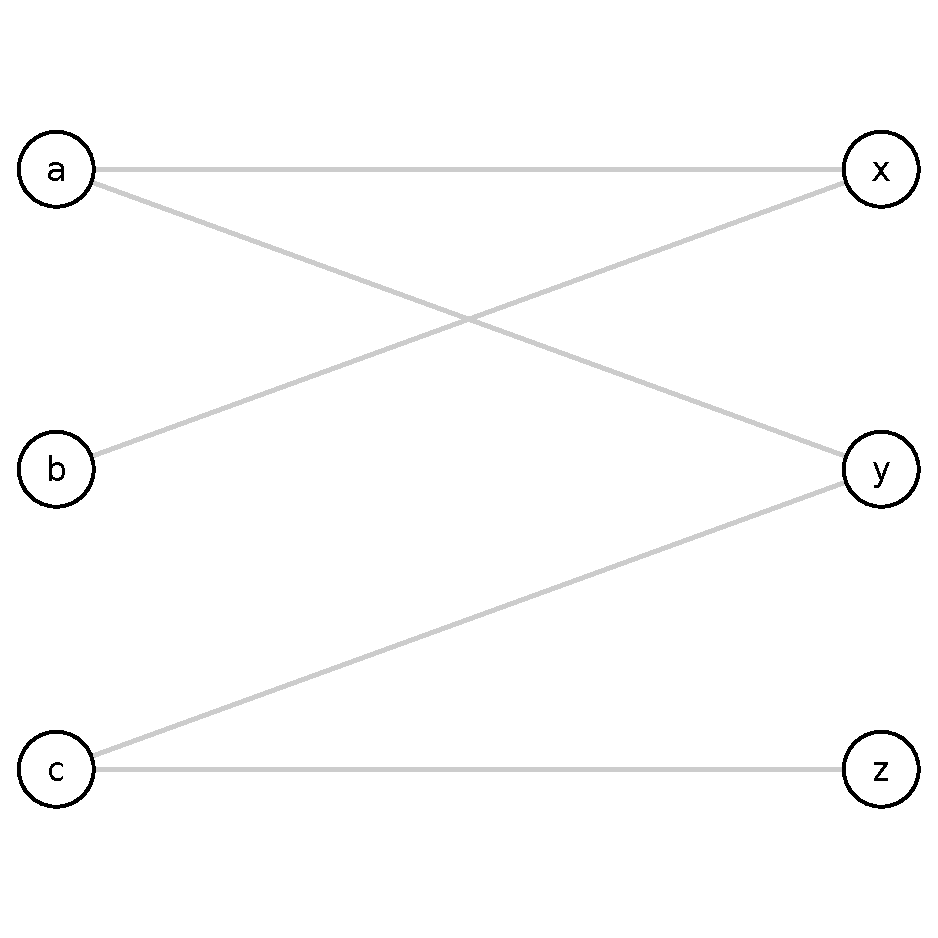
\includegraphics[width=0.46\textwidth]{python/lec09/matching/matching-0.pdf}\\[2pt]{\scriptsize Шаг 0. Сеть с фиктивными $S$ и $F$}} &
\shortstack{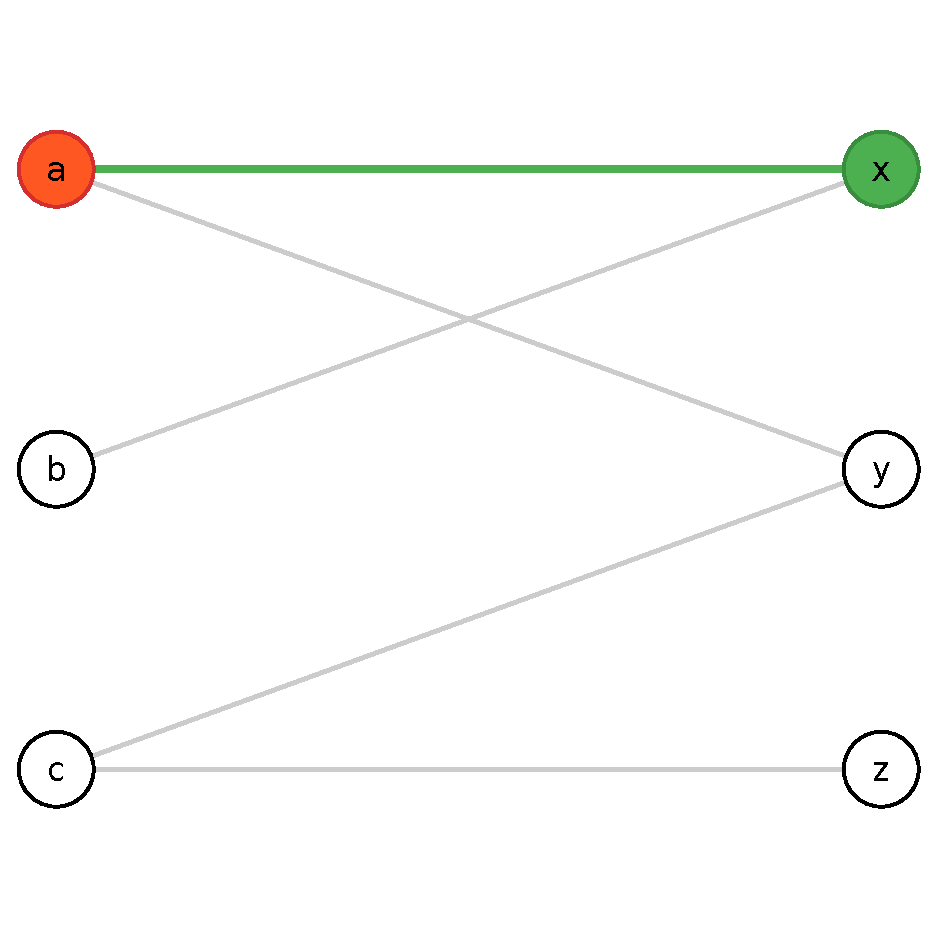
\includegraphics[width=0.46\textwidth]{python/lec09/matching/matching-1.pdf}\\[2pt]{\scriptsize Шаг 1. Путь 1: $S, B, \beta, F$}} \\
\end{tabular}\end{center}
\begin{center}\begin{tabular}{cc}
\shortstack{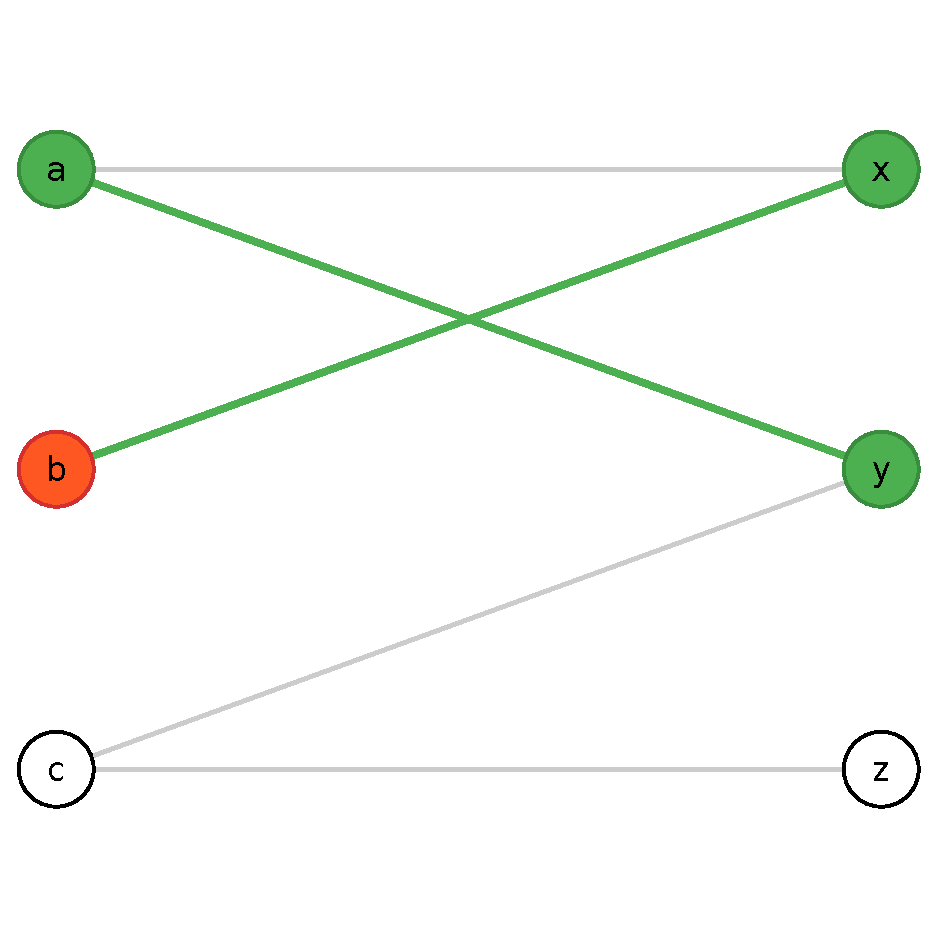
\includegraphics[width=0.46\textwidth]{python/lec09/matching/matching-2.pdf}\\[2pt]{\scriptsize Шаг 2. $B\beta$ развёрнуто: $\{B\beta\}$}} &
\shortstack{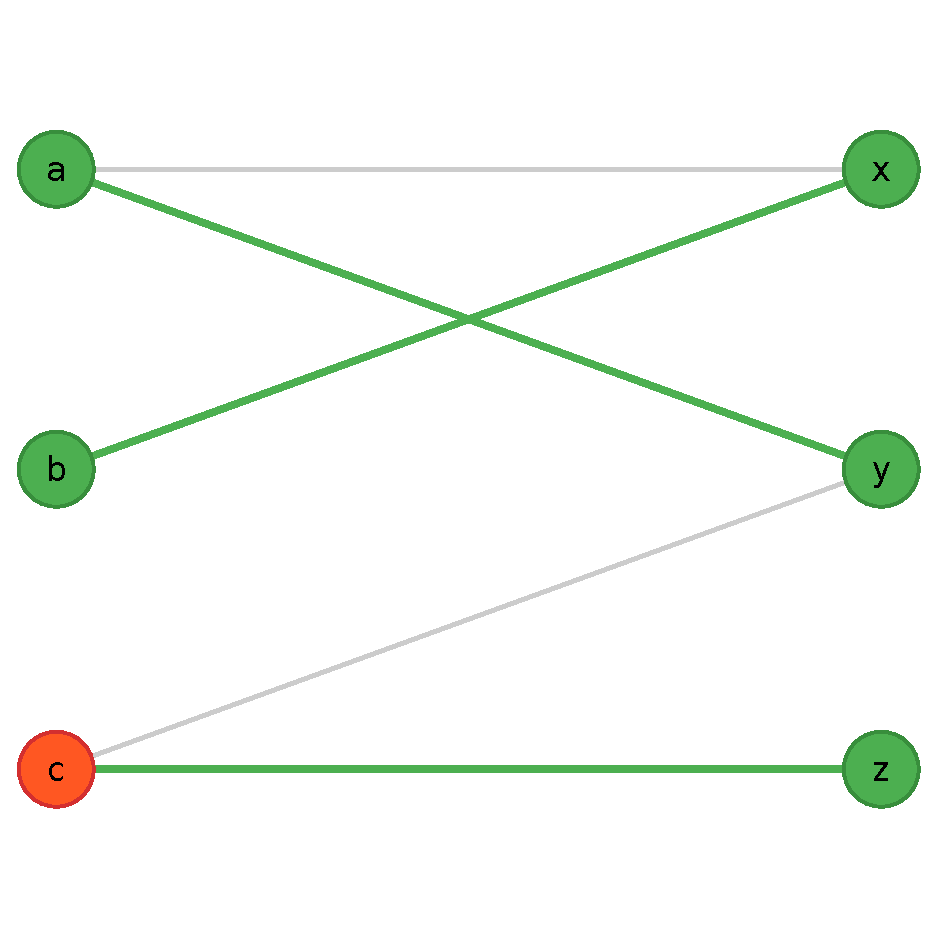
\includegraphics[width=0.46\textwidth]{python/lec09/matching/matching-3.pdf}\\[2pt]{\scriptsize Шаг 3. Путь 2: $S, C, \beta, B, \alpha, F$}} \\
\end{tabular}\end{center}
\begin{center}\begin{tabular}{cc}
\shortstack{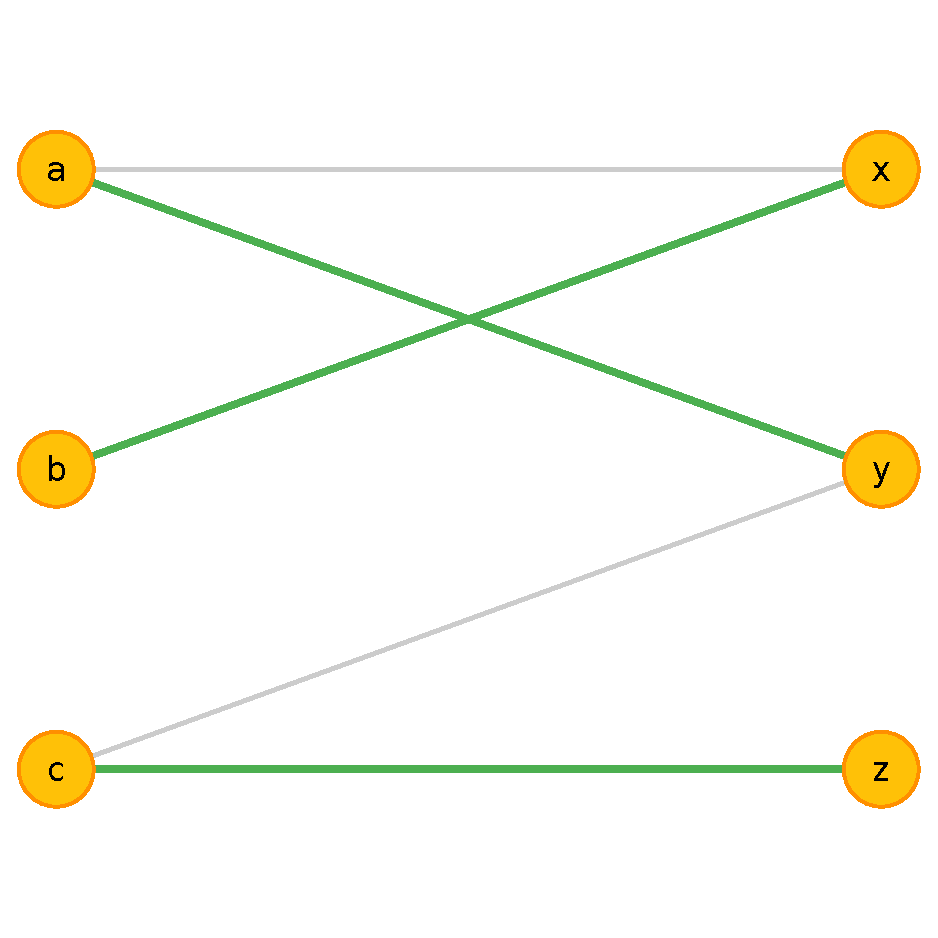
\includegraphics[width=0.46\textwidth]{python/lec09/matching/matching-4.pdf}\\[2pt]{\scriptsize Шаг 4. $\beta$ перешла к $C$, $B$ получил $\alpha$}} &
\shortstack{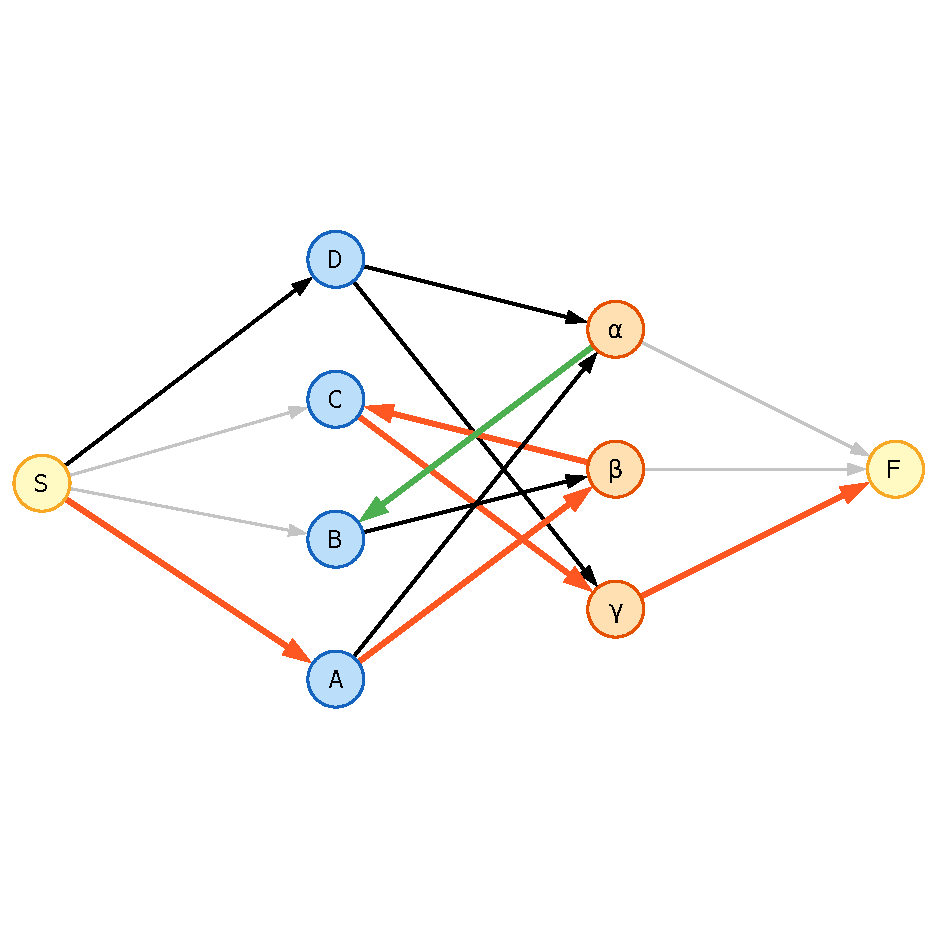
\includegraphics[width=0.46\textwidth]{python/lec09/matching/matching-5.pdf}\\[2pt]{\scriptsize Шаг 5. Путь 3: $S, A, \beta, C, \gamma, F$}} \\
\end{tabular}\end{center}
\begin{center}
\shortstack{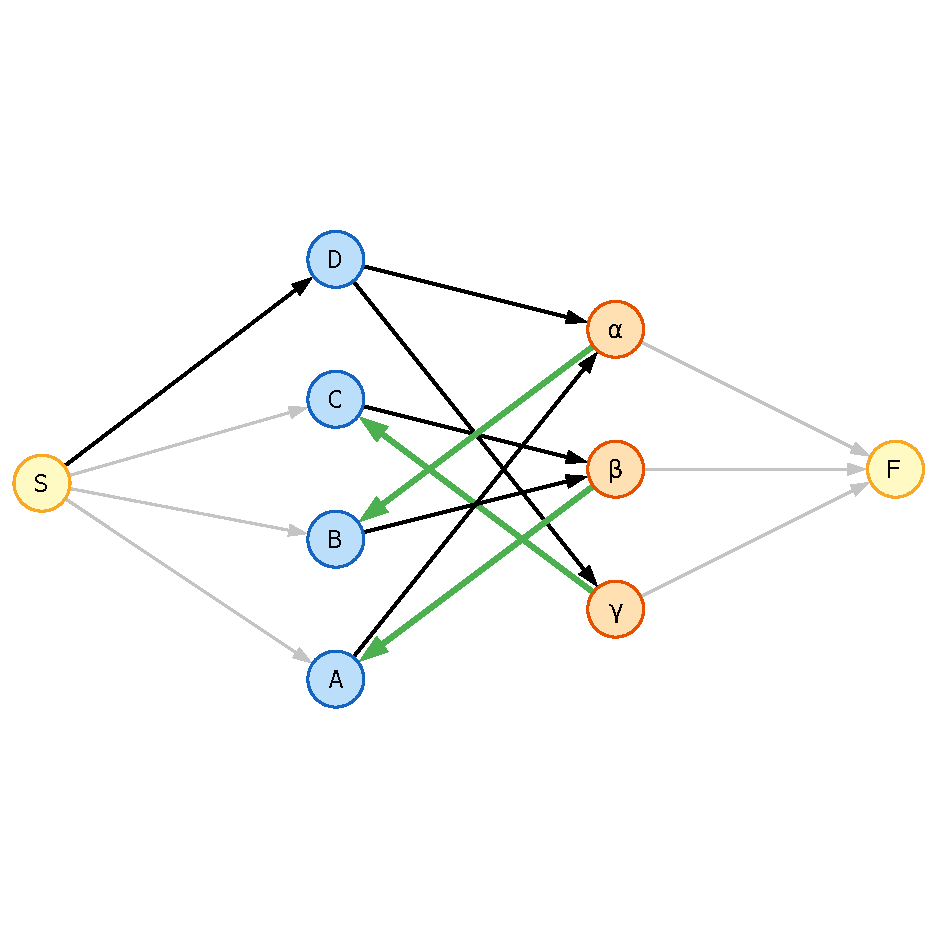
\includegraphics[width=0.5\textwidth]{python/lec09/matching/matching-6.pdf}\\[2pt]{\scriptsize Шаг 6. Итог: $\{A\beta, B\alpha, C\gamma\}$, путей $S \to F$ больше нет}}
\end{center}

\medskip
\textbf{Упр.} Почему паросочетание наибольшее?

\textit{Ответ (идея, лемма Бержа).} Паросочетание наибольшее
$\Leftrightarrow$ для него нет увеличивающего пути (чередующегося пути
между двумя свободными вершинами). Алгоритм останавливается ровно тогда,
когда пути $S \to F$ нет, т.\,е. нет и увеличивающего пути. Если бы
существовало паросочетание $\hat E'$ с $|\hat E'| > |\hat E|$, то в
симметрической разности $\hat E \,\Delta\, \hat E'$ (каждая вершина
задета не более чем двумя рёбрами --- это набор путей и чётных циклов)
нашлась бы компонента-путь, где рёбер $\hat E'$ больше, чем рёбер
$\hat E$, --- это и есть увеличивающий путь для $\hat E$. Противоречие.
\end{algo}

% ============================================================
% ЗАДАЧА О МАКСИМАЛЬНОМ ПОТОКЕ В СЕТИ
% ============================================================

\subsection*{Задача о максимальном потоке в сети}

\begin{defn}{Сеть}{network}
$G(V, E)$ --- \textbf{сеть}: \quad (орграф)
\begin{itemize}
  \item \textbf{исток:} $S$ --- нет входящих рёбер!
  \item \textbf{сток/устье:} $F$ --- нет исходящих рёбер!
\end{itemize}

$\sigma\colon E \to \mathbb{R}_{\geq 0}$ \quad (пропускная способность, пока на рёбрах).
\end{defn}

\begin{defn}{Поток}{flow}
\textbf{Поток:} $f\colon E \to \mathbb{R}$, свойства:
\begin{enumerate}
  \item $0 \leq f(e) \leq \sigma(e)$
  \item \textbf{Условие балансировки:}
        $\forall\, v \in V \setminus \{S, F\}$:\;
        $\displaystyle\sum_{\substack{e\colon u \to v \\ u \in V}} f(e) = 
         \displaystyle\sum_{\substack{e\colon v \to w \\ w \in V}} f(e)$

        \quad (поток входящий = поток исходящий)
\end{enumerate}
\end{defn}

\begin{defn}{Мощность потока}{flow-value}
\textbf{Мощность потока} $|f|$ = суммарное количество перемещаемого в единицу времени
(всё, что вытекает из $S$).

$|f| \to \max$

\textbf{Поток --- функция, НЕ число!}
\end{defn}

\medskip
\exhead{Пример.} Сеть с пропускными способностями (подпись ребра ---
$f/\sigma$, т.\,е. <<поток / пропускная способность>>):

\begin{center}
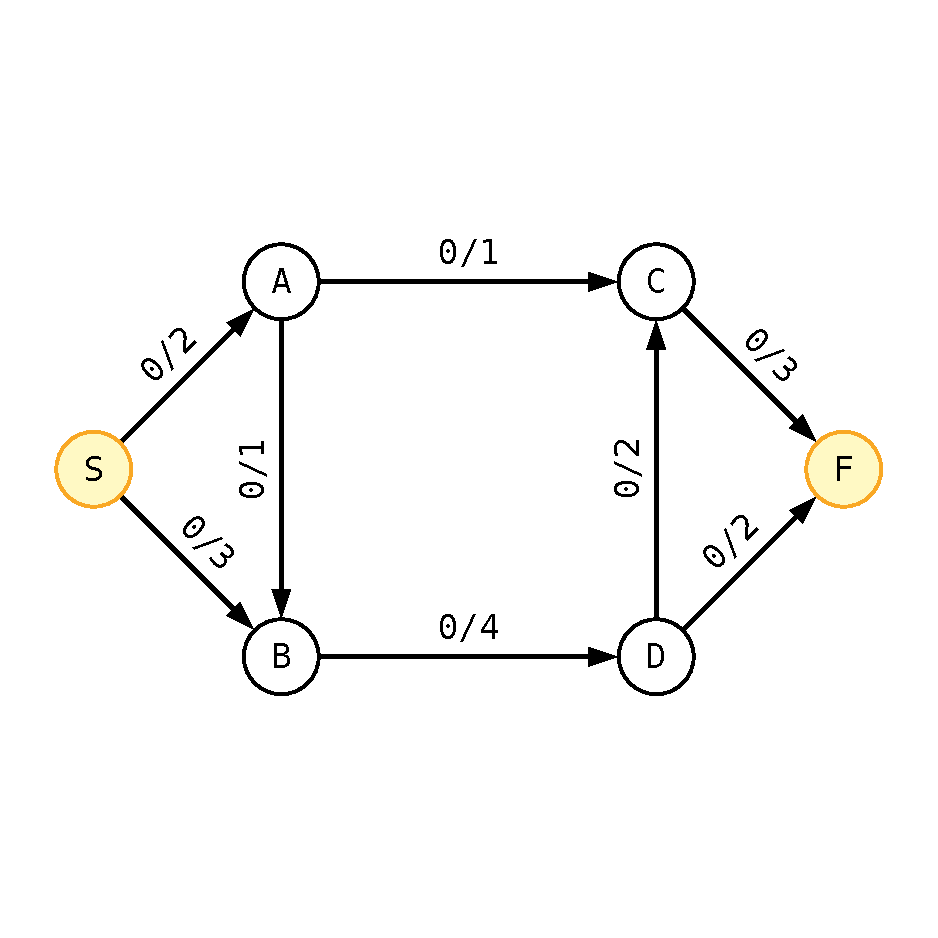
\includegraphics[width=0.5\textwidth]{python/lec09/flowexample/flowex-0.pdf}
\end{center}

Ищем пути из $S$ в $F$ и пускаем по каждому максимум возможного ---
\emph{минимум остаточных пропускных способностей рёбер пути} (самое
<<узкое горлышко>> пути ограничивает весь путь):

\begin{enumerate}
  \item путь $S, B, D, F$: остатки рёбер $3, 4, 2$, узкое место ---
        $DF$, $\min = 2$ --- пускаем $2$;
  \item путь $S, A, C, F$: остатки $2, 1, 3$, узкое место $AC$,
        $\min = 1$ --- пускаем $1$;
  \item путь $S, A, B, D, C, F$: остатки $1, 1, 2, 2, 2$, $\min = 1$
        --- пускаем $1$;
  \item путь $S, B, D, C, F$: остатки $1, 2, 1, 1$, $\min = 1$ ---
        пускаем $1$.
\end{enumerate}

\begin{center}\begin{tabular}{cc}
\shortstack{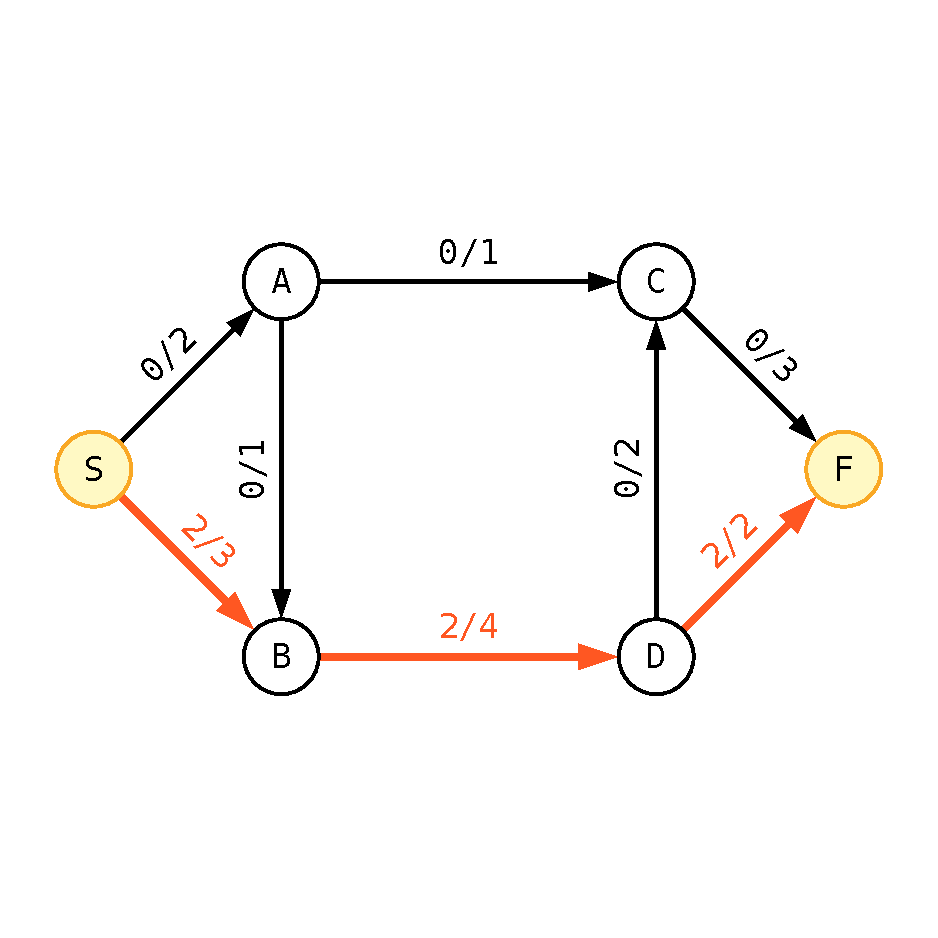
\includegraphics[width=0.46\textwidth]{python/lec09/flowexample/flowex-1.pdf}\\[2pt]{\scriptsize Путь 1: $S{,}B{,}D{,}F$, $\min = 2$, $|f| = 2$}} &
\shortstack{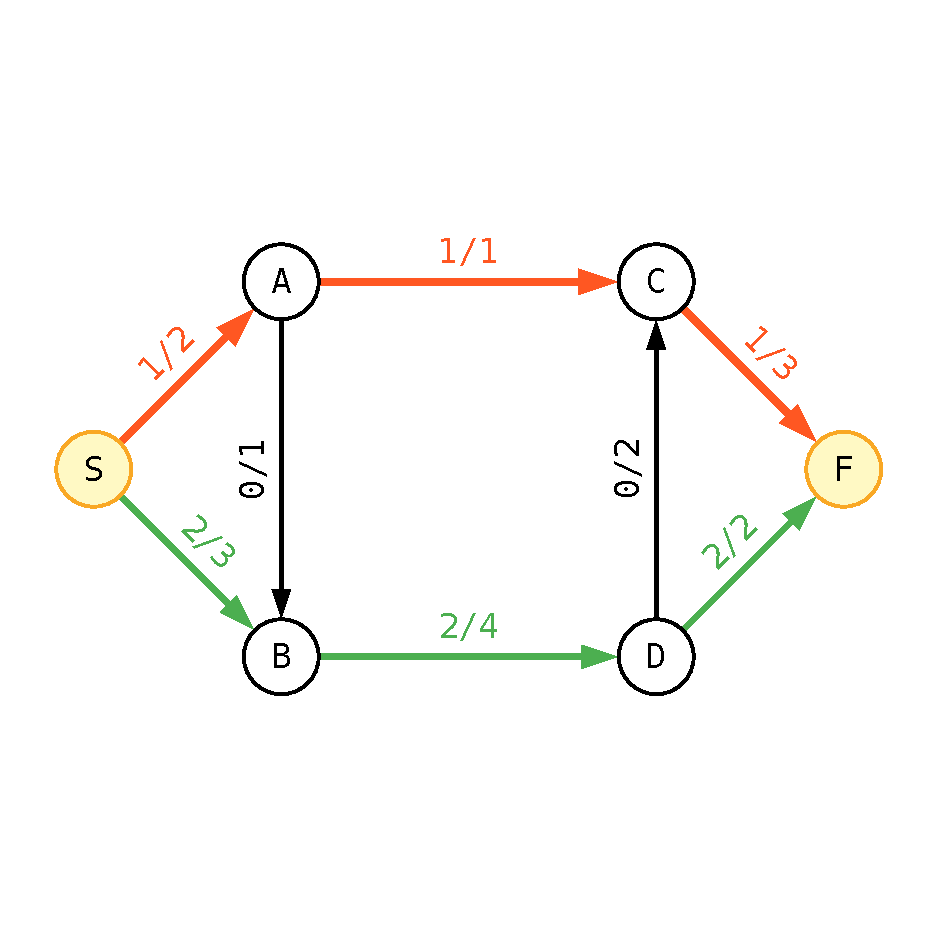
\includegraphics[width=0.46\textwidth]{python/lec09/flowexample/flowex-2.pdf}\\[2pt]{\scriptsize Путь 2: $S{,}A{,}C{,}F$, $\min = 1$, $|f| = 3$}} \\
\end{tabular}\end{center}
\begin{center}\begin{tabular}{cc}
\shortstack{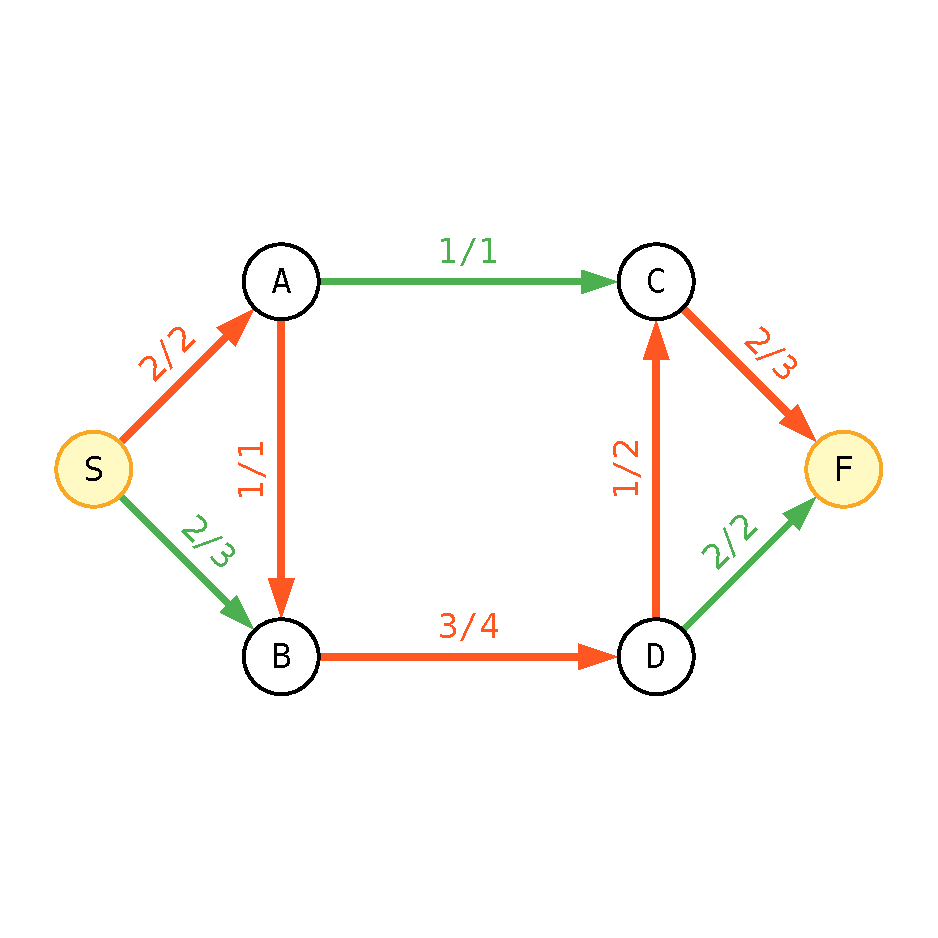
\includegraphics[width=0.46\textwidth]{python/lec09/flowexample/flowex-3.pdf}\\[2pt]{\scriptsize Путь 3: $S{,}A{,}B{,}D{,}C{,}F$, $\min = 1$, $|f| = 4$}} &
\shortstack{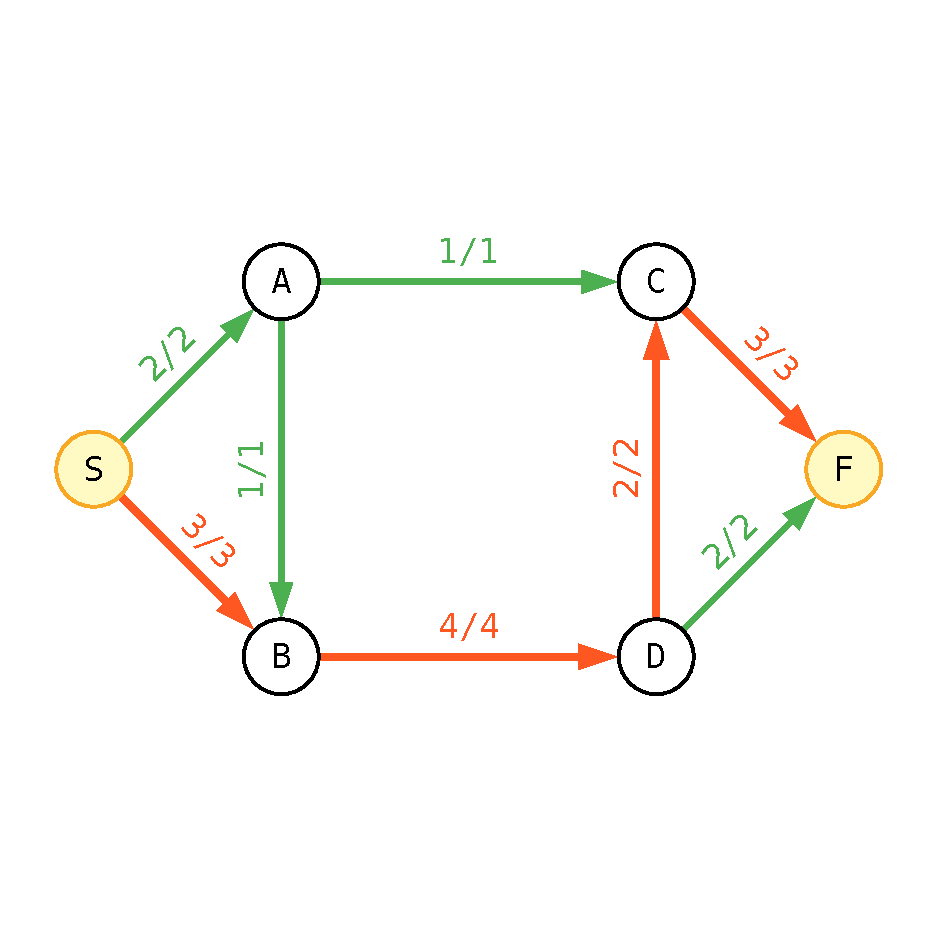
\includegraphics[width=0.46\textwidth]{python/lec09/flowexample/flowex-4.pdf}\\[2pt]{\scriptsize Путь 4: $S{,}B{,}D{,}C{,}F$, $\min = 1$, $|f| = 5$}} \\
\end{tabular}\end{center}
\begin{center}
\shortstack{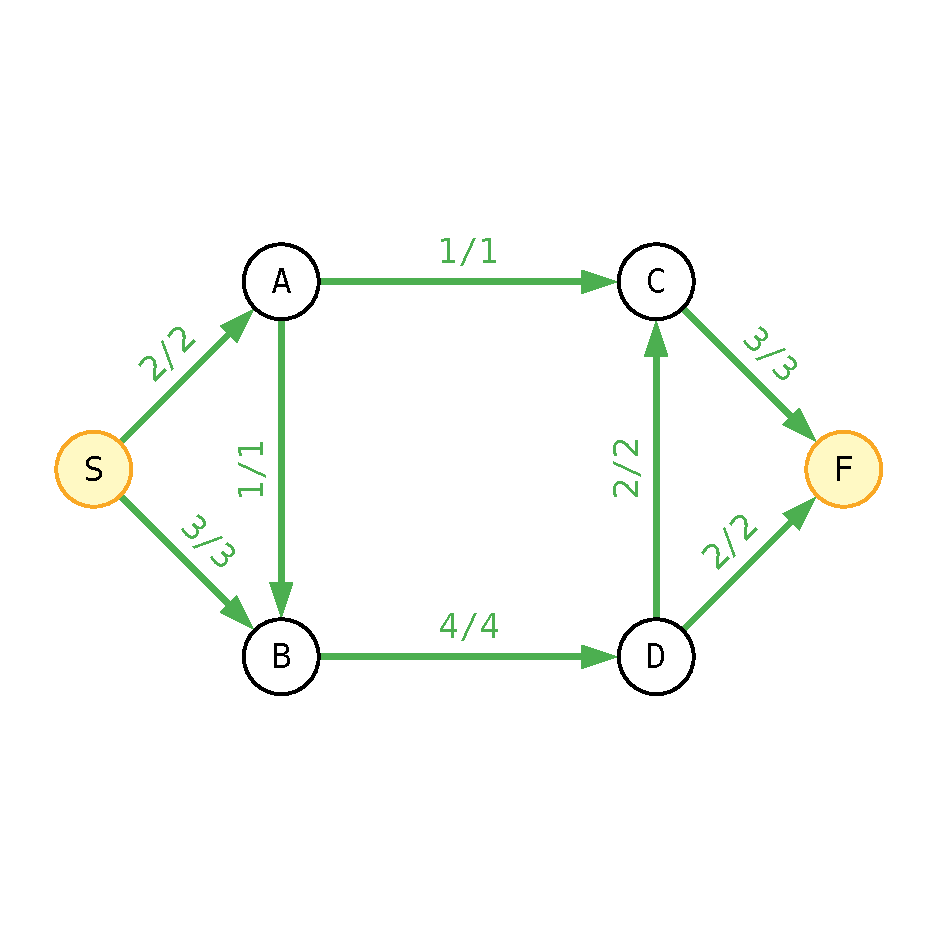
\includegraphics[width=0.5\textwidth]{python/lec09/flowexample/flowex-5.pdf}\\[2pt]{\scriptsize Итог: $|f| = 5$, оба ребра из $S$ насыщены}}
\end{center}

После каждого пути остаточные веса пересчитываются; при насыщении ребра
в общем случае добавляется фиктивное обратное ребро с остаточной
ёмкостью (подробно --- в лекции про алгоритм Форда--Фалкерсона).

\medskip
\textbf{Итог:}
условие балансировки выполняется в каждой внутренней вершине, и
$|f| = 2 + 1 + 1 + 1 = 5$ --- максимум: оба ребра из истока
($S{\to}A$ и $S{\to}B$) насыщены, больше из $S$ вытечь не может.

% ============================================================
\begin{task}{Наибольшее паросочетание в двудольном графе}{matching-task}
\textbf{Условие.} Дан двудольный граф с долями $\{a,b,c\}$ и $\{x,y,z\}$ и
рёбрами
\[
  a\!-\!x,\quad a\!-\!y,\quad b\!-\!x,\quad c\!-\!y,\quad c\!-\!z.
\]
Найдите наибольшее паросочетание (алгоритм Куна, поиск увеличивающих путей).

\begin{center}
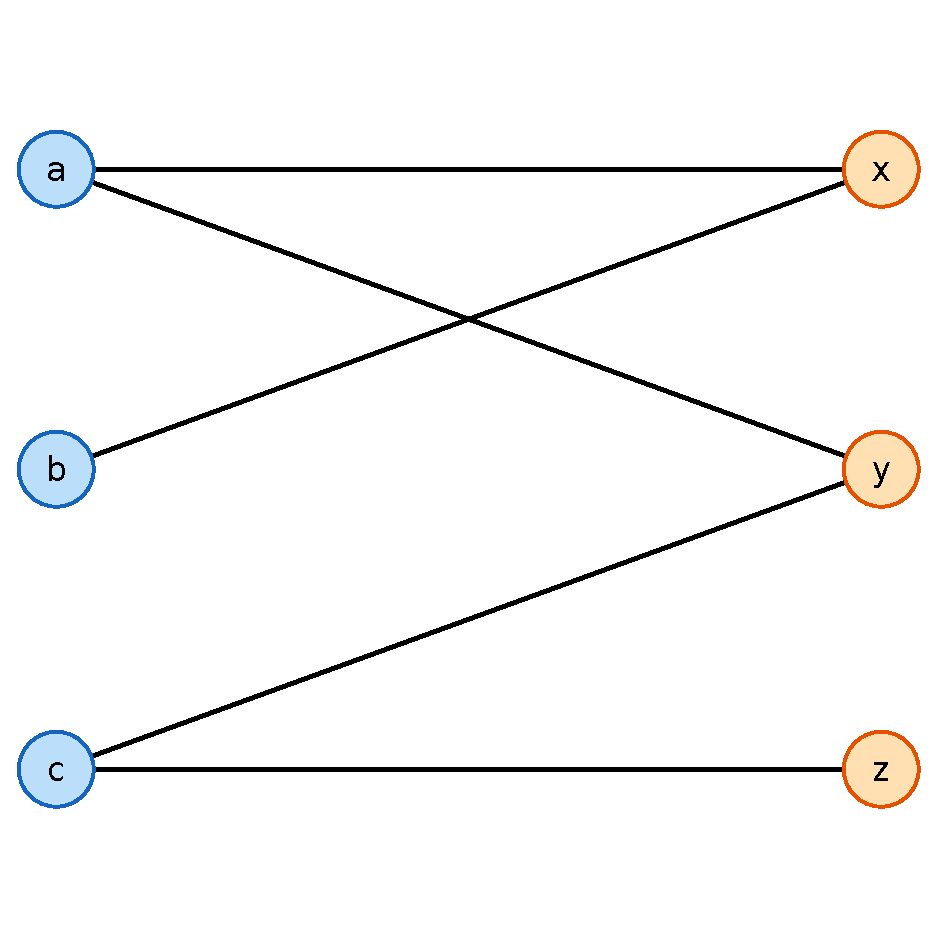
\includegraphics[width=0.4\textwidth]{figures/match-example.pdf}
\end{center}

\smallskip
\textbf{Решение.} Паросочетание --- набор попарно несмежных рёбер. Алгоритм Куна
по очереди пытается насытить каждую вершину левой доли, ища увеличивающий путь
(чередующий путь из свободной вершины в свободную).
\begin{enumerate}
  \item $a$: свободно ребро $a\!-\!x$ $\Rightarrow$ паросочетание $\{a\!-\!x\}$.
  \item $b$: единственное ребро $b\!-\!x$, но $x$ занят $a$. Ищем увеличивающий
        путь: $b\!-\!x$, $x$ занят $a$, у $a$ есть альтернатива $a\!-\!y$ ($y$
        свободна). Перекладываем: $a\!-\!y,\ b\!-\!x$. Паросочетание
        $\{a\!-\!y,\ b\!-\!x\}$.
  \item $c$: ребро $c\!-\!y$ ведёт к занятому $y$; пробуем $c\!-\!z$ ($z$
        свободна) $\Rightarrow$ добавляем $c\!-\!z$. Паросочетание
        $\{a\!-\!y,\ b\!-\!x,\ c\!-\!z\}$.
\end{enumerate}
Все три вершины левой доли насыщены --- паросочетание совершенное, его размер
$3$ (больше быть не может, так как доли по $3$ вершины).

\begin{center}
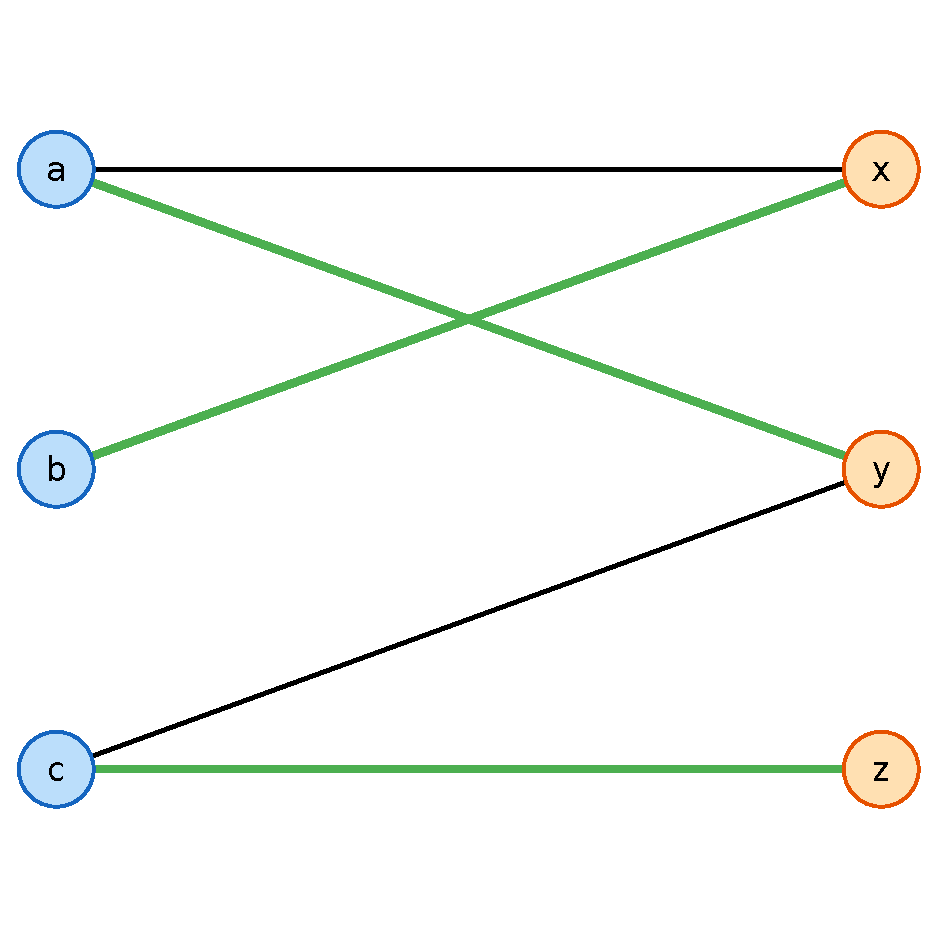
\includegraphics[width=0.4\textwidth]{figures/task-matching-sol.pdf}
\end{center}

\textbf{Ответ.} Наибольшее паросочетание: $\{a\!-\!y,\ b\!-\!x,\ c\!-\!z\}$,
размер $3$ (совершенное).
\end{task}


% ===========================================================
%  Лекция 10. Задача о максимальном потоке.
%             Алгоритм Форда—Фалкерсона
% ===========================================================

\chapter{Лекция 10. Алгоритм Форда—Фалкерсона}

% -----------------------------------------------------------
% Постановка задачи
% -----------------------------------------------------------
\subsection*{Постановка задачи}

\textbf{Дано:} сеть $G(V, E)$,\quad $\sigma\colon E \to \mathbb{R}$ --- пропускная
способность рёбер.

\textbf{Найти:} один из максимальных потоков $f\colon E \to \mathbb{R}_{\geq 0}$,
т.\,е. поток наибольшей мощности $|f|$.

\medskip
\noindent
Напомним (лекция~9): поток $f$ удовлетворяет ограничению $0 \le f(e) \le \sigma(e)$
и условию балансировки во всех вершинах, кроме истока $S$ и стока $F$.

% -----------------------------------------------------------
% Остаточная сеть
% -----------------------------------------------------------
\subsection*{Остаточная сеть}

\begin{defn}{Остаточная пропускная способность}{residual-capacity}
Для ребра $e = \overline{uv}$ и текущего потока $f$ \textbf{остаточная пропускная
способность} $\tilde{\sigma}(e)$ показывает, сколько ещё можно пропустить по~$e$.
Вводится обратное (фиктивное) ребро $\operatorname{inv}(e) = \overline{vu}$, и
\[
  \tilde{\sigma}(e) + \tilde{\sigma}(\operatorname{inv}(e)) = \sigma(e).
\]
Изначально $\tilde{\sigma}(e) := \sigma(e)$, $\tilde{\sigma}(\operatorname{inv}(e)) := 0$.
\end{defn}

\begin{defn}{Остаточная сеть}{residual-network}
\textbf{Остаточная сеть} --- сеть на тех же вершинах, рёбрами которой служат все рёбра
с положительной остаточной пропускной способностью $\tilde{\sigma}(e) > 0$
(включая обратные рёбра $\operatorname{inv}(e)$).
\end{defn}

\begin{defn}{Исчерпанное (насыщенное) ребро}{saturated-edge}
\textbf{Исчерпанное ребро} --- ребро с нулевой остаточной пропускной способностью
$\tilde{\sigma}(e) = 0$ (поток по нему равен пропускной способности: $f(e) = \sigma(e)$).
\end{defn}

% -----------------------------------------------------------
% Разрезы
% -----------------------------------------------------------
\subsection*{Разрезы}

\begin{defn}{Разрез в сети}{cut}
\textbf{Разрез} в сети --- такой набор рёбер $\tilde{E} \subseteq E$, что удаление его
разрывает все пути $S \to F$, т.\,е. граф $G(V,\, E \setminus \tilde{E})$ теряет
связность между $S$ и $F$.

\medskip
\textbf{NB.} Любой мост --- разрез. Обычно рассматривают $\tilde{E}$, минимальный
по включению.
\end{defn}

\begin{defn}{Главный разрез}{main-cut}
\textbf{Главный разрез} --- разрез, при котором граф делится ровно на две части.
\end{defn}

\begin{defn}{Пропускная способность разреза}{cut-capacity}
Пропускная способность разреза $\tilde{E}$ --- сумма пропускных способностей его рёбер,
направленных из части истока в часть стока:
$\displaystyle \sigma(\tilde{E}) = \sum_{e \in \tilde{E}} \sigma(e)$.
\end{defn}

% -----------------------------------------------------------
% Алгоритм
% -----------------------------------------------------------
\subsection*{Алгоритм Форда—Фалкерсона}

\begin{algo}{Форда—Фалкерсона (поиск максимального потока)}{ford-fulkerson}
\textbf{Инициализация:}
\[
  \forall\, e \in E\colon\; f(e) := 0, \qquad
  \forall\, e \in E\colon\; \tilde{\sigma}(e) := \sigma(e).
\]

\textbf{Шаг.} Пока в остаточной сети существует путь $S \xrightarrow{\;e_1\;} \cdots
\xrightarrow{\;e_t\;} F$ (дополняющий путь):

\begin{enumerate}
  \item Находим узкое место пути ---
        $\displaystyle \delta := \min_{1 \le i \le t} \tilde{\sigma}(e_i)$,
        и увеличиваем поток вдоль всего пути:
        $\forall\, e_i\colon f(e_i) \mathrel{+}= \delta$.

  \item Перестраиваем остаточную сеть: для каждого ребра пути
        \[
          \tilde{\sigma}_{\text{new}}(e_i) = \tilde{\sigma}_{\text{old}}(e_i) - \delta,
          \qquad
          \tilde{\sigma}_{\text{new}}(\operatorname{inv}(e_i))
            = \tilde{\sigma}_{\text{old}}(\operatorname{inv}(e_i)) + \delta.
        \]
\end{enumerate}

\textbf{Выход:} когда дополняющих путей больше нет, текущий поток $f$ --- максимальный.

\medskip
\noindent\textbf{Пример.} Сеть с вершинами $S, A, B, C, D, F$ (та же, что
в лекции~9). Подпись каждого ребра --- $f/\sigma$
(поток\,/\,пропускная способность). Дополняющий путь выделен оранжевым,
рёбра с положительным потоком --- зелёным. Пути ищем поиском в ширину
(кратчайший по числу рёбер --- вариант Эдмондса--Карпа).

\begin{center}\begin{tabular}{cc}
\shortstack{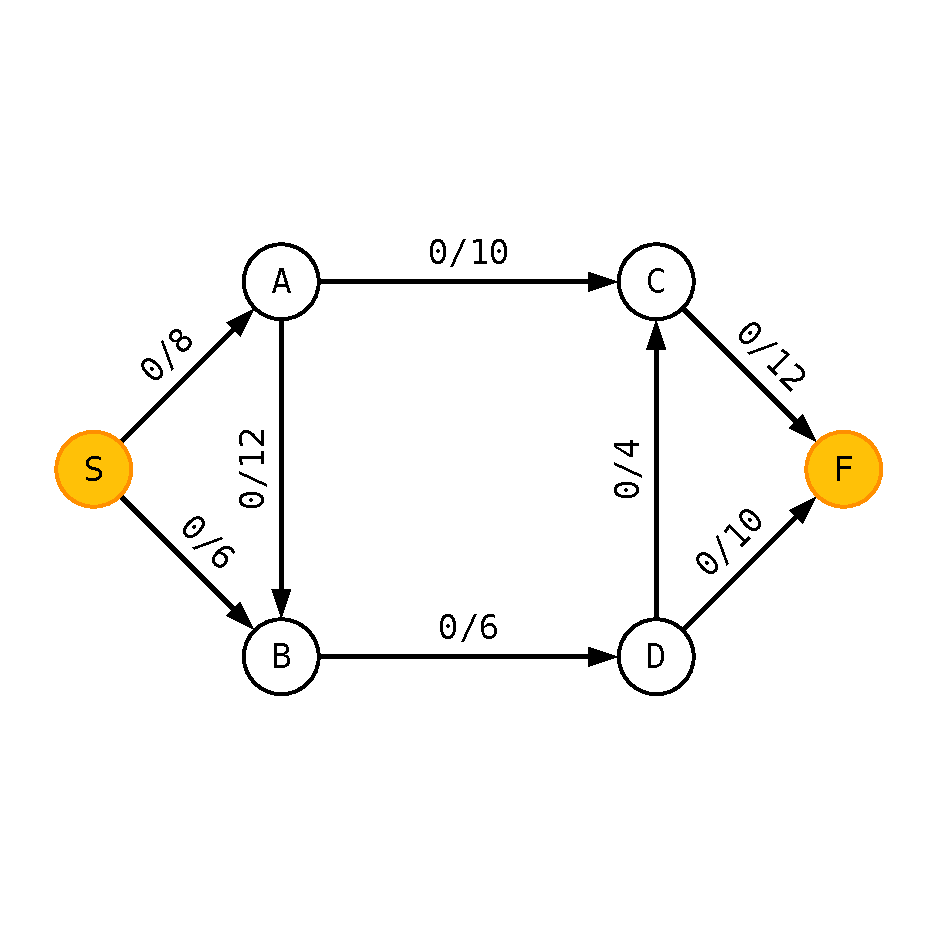
\includegraphics[width=0.46\textwidth]{python/lec10/ford_fulkerson/ford_fulkerson-0.pdf}\\[2pt]{\scriptsize Шаг 0. Инициализация: $f \equiv 0$, $\tilde\sigma = \sigma$}} &
\shortstack{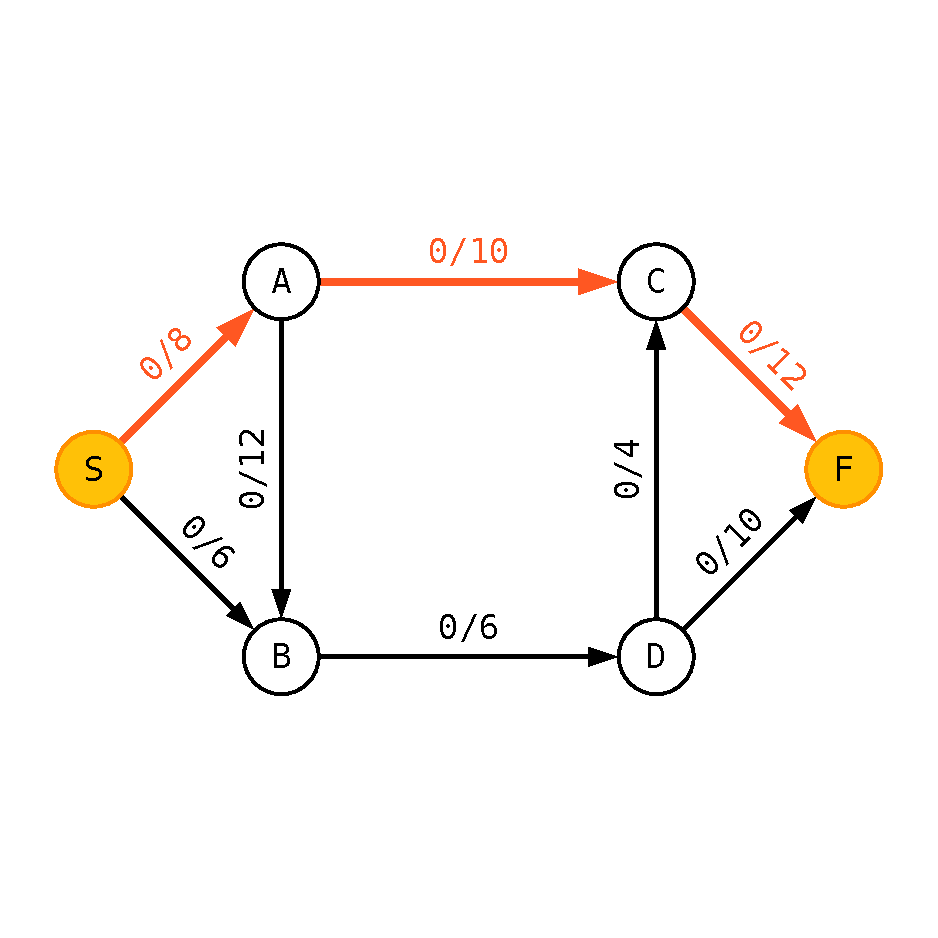
\includegraphics[width=0.46\textwidth]{python/lec10/ford_fulkerson/ford_fulkerson-1.pdf}\\[2pt]{\scriptsize Шаг 1. Путь $S{\to}A{\to}C{\to}F$, $\delta = \min(2,1,3) = 1$}} \\
\end{tabular}\end{center}
\begin{center}\begin{tabular}{cc}
\shortstack{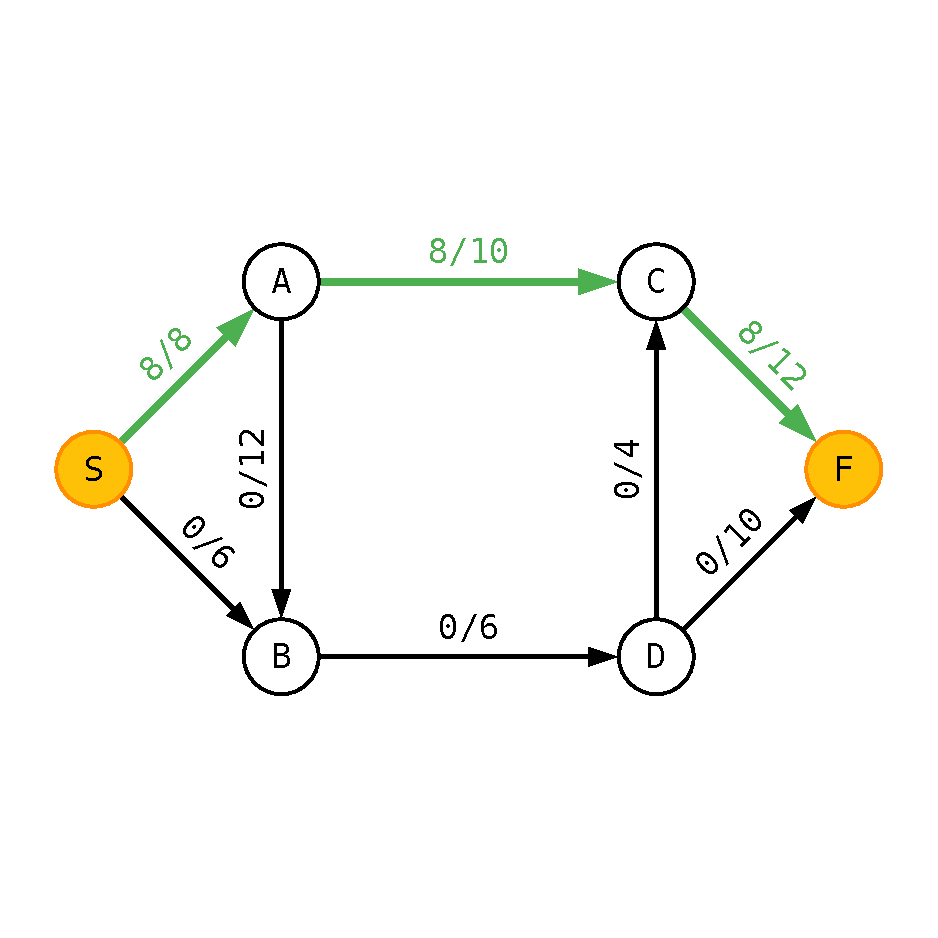
\includegraphics[width=0.46\textwidth]{python/lec10/ford_fulkerson/ford_fulkerson-2.pdf}\\[2pt]{\scriptsize Шаг 2. Поток проведён: $|f| = 1$; $A{\to}C$ исчерпано}} &
\shortstack{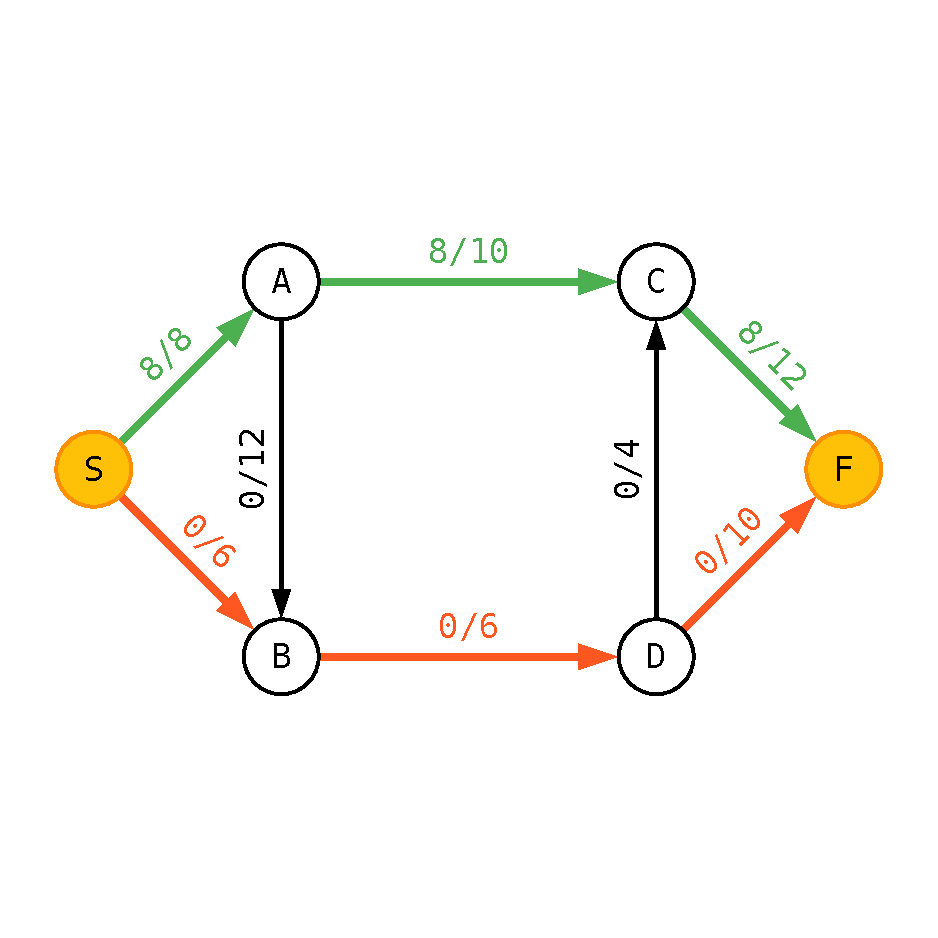
\includegraphics[width=0.46\textwidth]{python/lec10/ford_fulkerson/ford_fulkerson-3.pdf}\\[2pt]{\scriptsize Шаг 3. Путь $S{\to}B{\to}D{\to}F$, $\delta = \min(3,4,2) = 2$}} \\
\end{tabular}\end{center}
\begin{center}\begin{tabular}{cc}
\shortstack{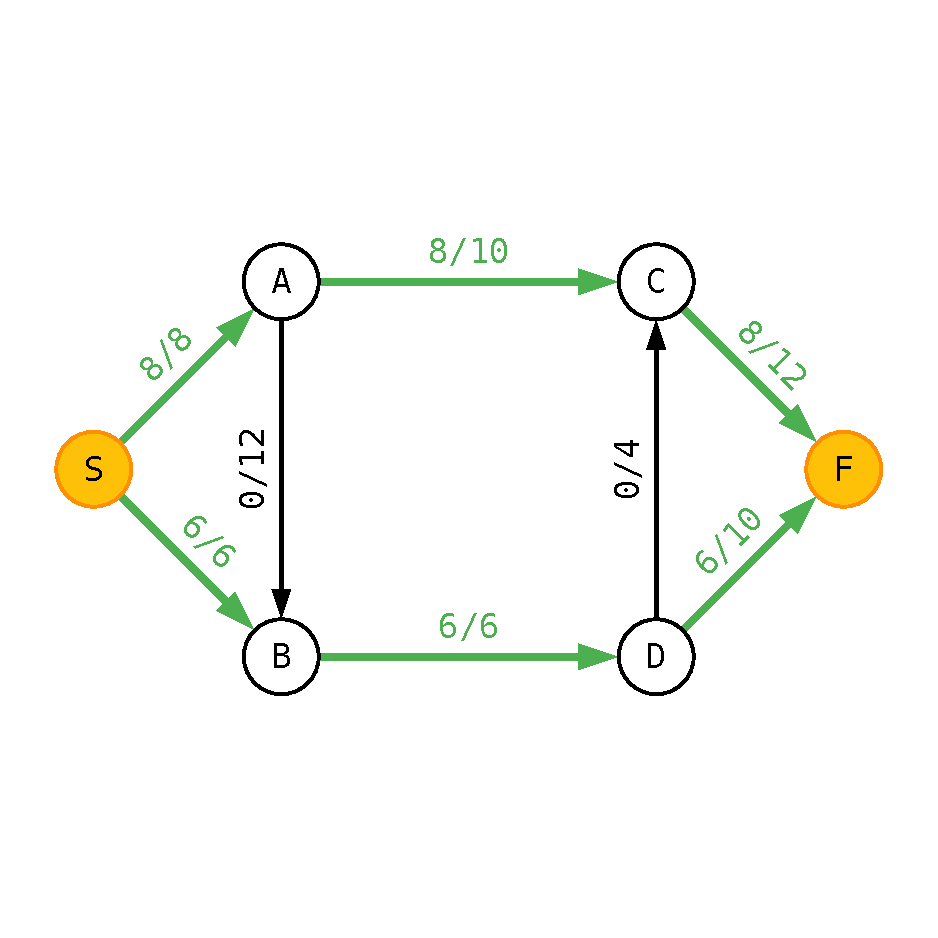
\includegraphics[width=0.46\textwidth]{python/lec10/ford_fulkerson/ford_fulkerson-4.pdf}\\[2pt]{\scriptsize Шаг 4. $|f| = 3$; ребро $D{\to}F$ исчерпано}} &
\shortstack{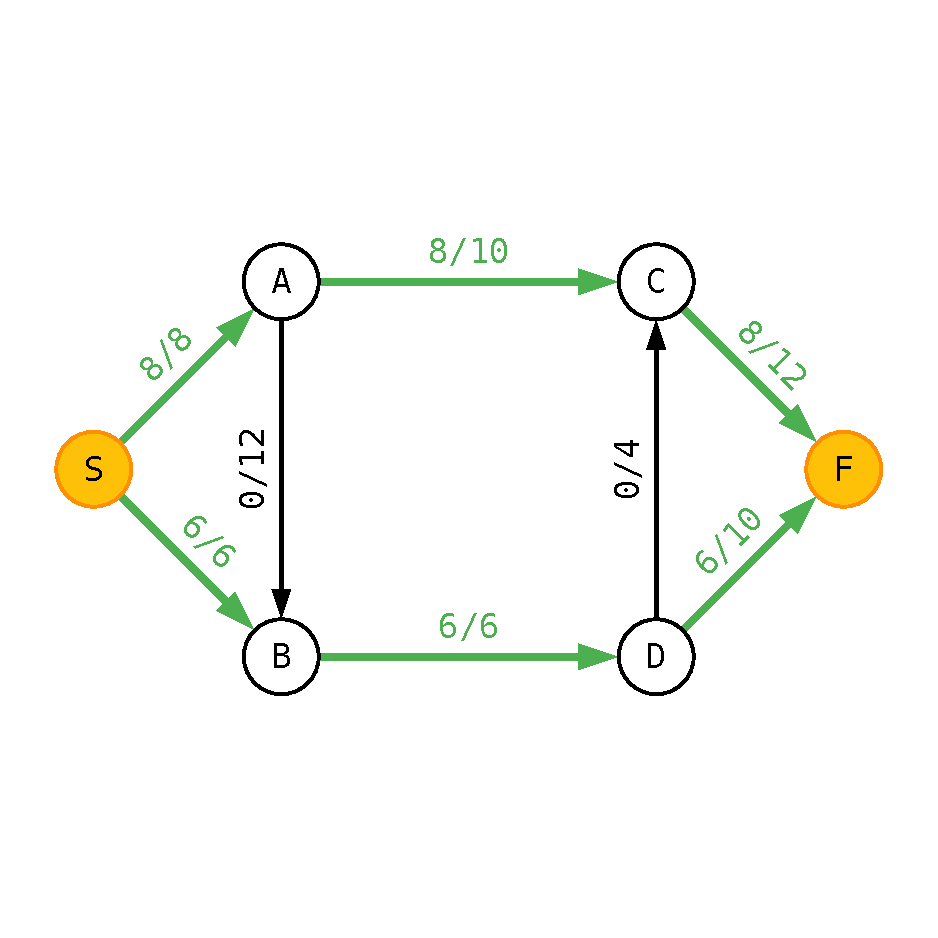
\includegraphics[width=0.46\textwidth]{python/lec10/ford_fulkerson/ford_fulkerson-5.pdf}\\[2pt]{\scriptsize Шаг 5. Путь $S{\to}B{\to}D{\to}C{\to}F$, $\delta = 1$}} \\
\end{tabular}\end{center}
\begin{center}\begin{tabular}{cc}
\shortstack{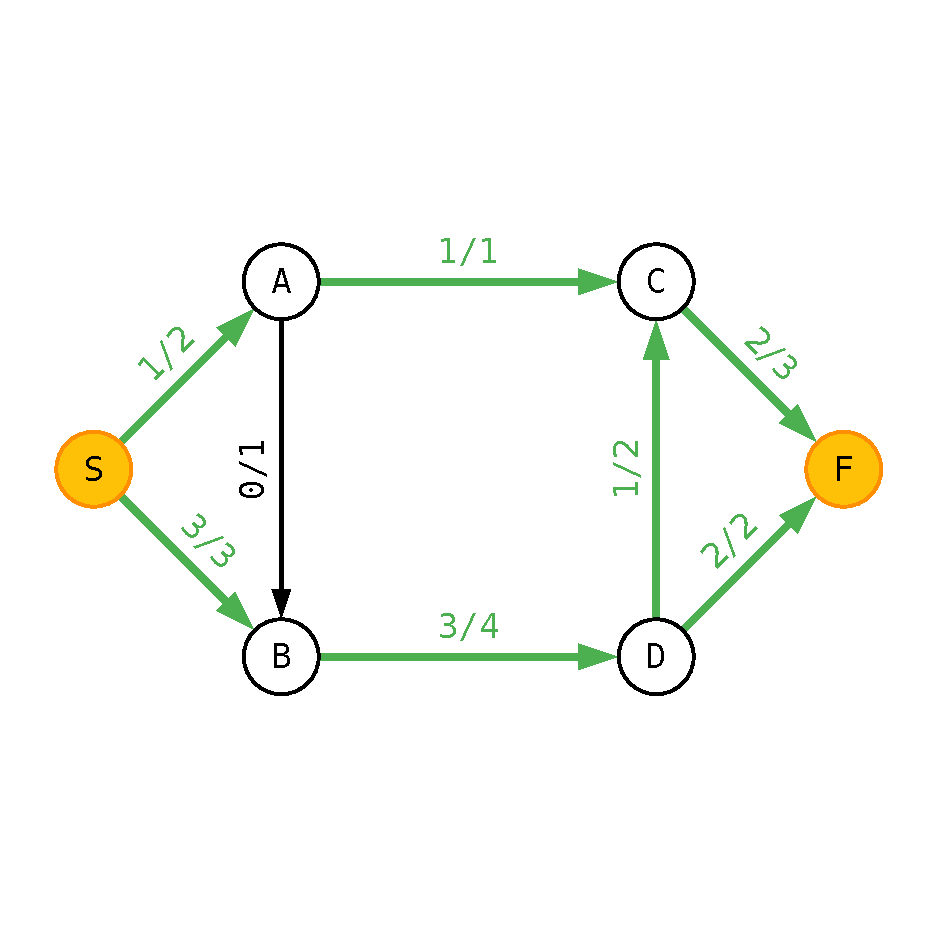
\includegraphics[width=0.46\textwidth]{python/lec10/ford_fulkerson/ford_fulkerson-6.pdf}\\[2pt]{\scriptsize Шаг 6. $|f| = 4$; ребро $S{\to}B$ исчерпано}} &
\shortstack{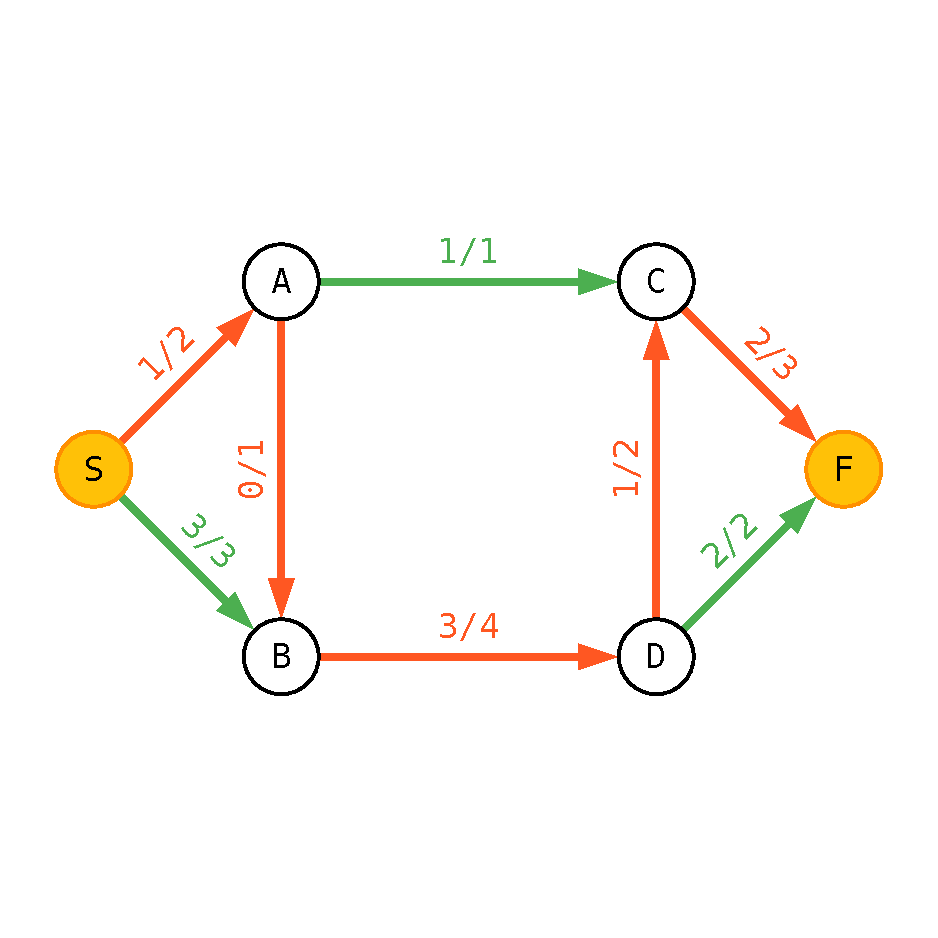
\includegraphics[width=0.46\textwidth]{python/lec10/ford_fulkerson/ford_fulkerson-7.pdf}\\[2pt]{\scriptsize Шаг 7. Путь $S{\to}A{\to}B{\to}D{\to}C{\to}F$, $\delta = 1$}} \\
\end{tabular}\end{center}
\begin{center}\begin{tabular}{cc}
\shortstack{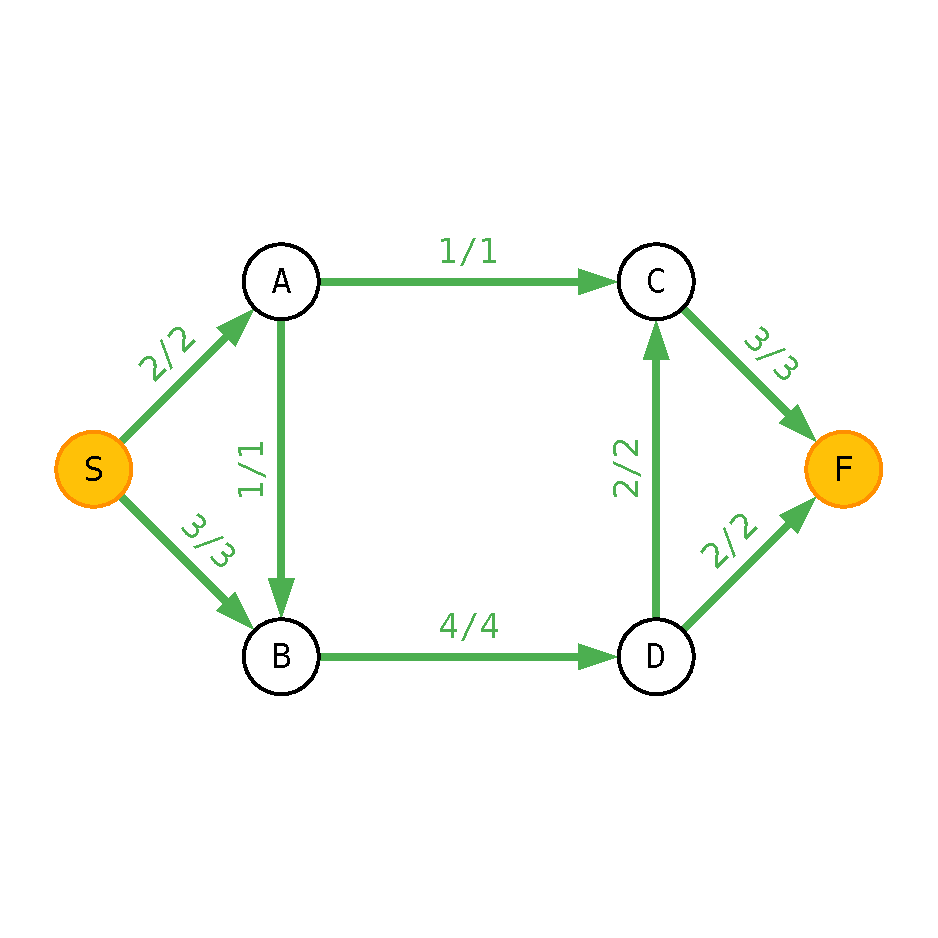
\includegraphics[width=0.46\textwidth]{python/lec10/ford_fulkerson/ford_fulkerson-8.pdf}\\[2pt]{\scriptsize Шаг 8. $|f| = 5$; ребро $S{\to}A$ исчерпано}} &
\shortstack{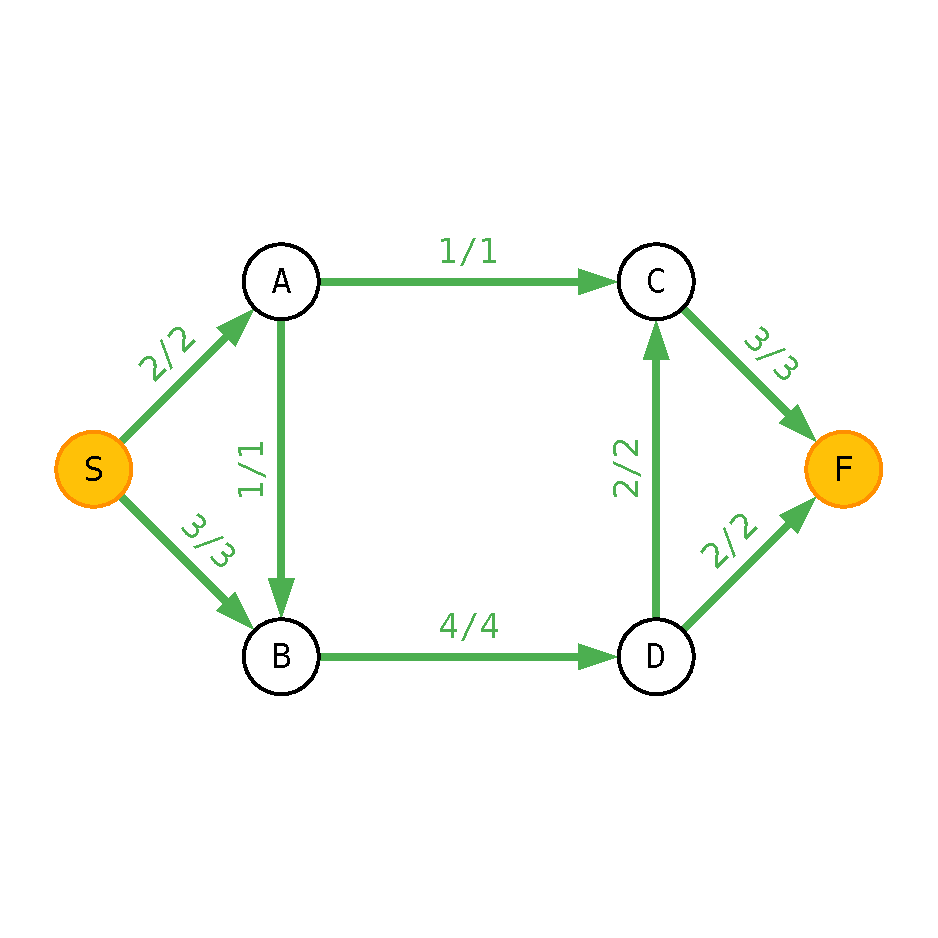
\includegraphics[width=0.46\textwidth]{python/lec10/ford_fulkerson/ford_fulkerson-9.pdf}\\[2pt]{\scriptsize Шаг 9. Путей $S \to F$ в остаточной сети нет: $|f|_{\max} = 5$}} \\
\end{tabular}\end{center}

\noindent\textit{Комментарии к шагам.} На каждом шаге величина потока
увеличивается на узкое место $\delta$ найденного пути: $1 + 2 + 1 + 1 = 5$.
После шага~8 оба ребра из истока ($S{\to}A$ и $S{\to}B$) исчерпаны:
в остаточной сети из $S$ не выходит ни одного ребра, дополняющих путей
нет --- алгоритм останавливается.

\medskip
\noindent\textbf{Проверка через разрез.} Набор рёбер
$\tilde E = \{S{\to}A,\; S{\to}B\}$ --- главный разрез
($\{S\}$ против остальных вершин) с пропускной способностью
$\sigma(\tilde E) = 2 + 3 = 5$. Мощность любого потока не превосходит
пропускной способности любого разреза, поэтому $|f| = 5 =
\sigma(\tilde E)$ --- поток максимален, а разрез минимален
(теорема Форда--Фалкерсона: $\max |f| = \min \sigma(\tilde E)$).
\end{algo}


% ===========================================================
%  Лекция 11. Задача о максимальном потоке в сети.
%             Метод проталкивания предпотока
% ===========================================================

\chapter{Лекция 11. Задача о максимальном потоке в сети}

\subsection*{Метод (алгоритм) проталкивания предпотока}

Идея метода: в отличие от Форда--Фалкерсона, который наращивает поток
целыми путями $S \to F$, здесь мы разрешаем вершинам временно
\emph{накапливать} лишний втекающий поток (избыток) и затем
<<проталкивать>> его дальше --- как вода, стекающая по каскаду
резервуаров разной высоты.

\begin{defn}{Предпоток}{predpotok}
Пусть $G$~--- сеть, $\sigma$~--- пропускная способность рёбер.

\textbf{Предпоток}~--- это функция $\tilde{f}\colon V \times V \to \mathbb{R}$, удовлетворяющая условиям:
\begin{enumerate}
  \item \textbf{Ограниченность:} $\forall\, e = uv\colon -\sigma(e) \le \tilde{f}(u,v) \le \sigma(e)$;
  \item \textbf{Кососимметричность:} $\forall\, u,v \in V\colon \tilde{f}(u,v) = -\tilde{f}(v,u)$;
  \item $\forall\, \nexists\, e = uv,\; e = vu \;\Rightarrow\; \tilde{f}(u,v) = 0$.
\end{enumerate}
В отличие от потока, условие балансировки \emph{не требуется}: в вершину
может втекать больше, чем вытекает.
\end{defn}

\begin{defn}{Эксцесс вершины}{excess}
\textbf{Эксцесс вершины} $\forall\, v \in V$:
\[
  \varepsilon(v) := \sum_{w \in P(v)} \tilde{f}(\overline{wv}) - \sum_{u \in \mathrm{Ch}(v)} \tilde{f}(\overline{vu}),
\]
где $P(v)$~--- родители, $\mathrm{Ch}(v)$~--- дети
(т.\,е.\ эксцесс --- это <<втекло минус вытекло>>).
\end{defn}

\textbf{NB.} Если $\forall\, v \in V \setminus \{S, F\}\colon \varepsilon(v) = 0$, то $\tilde{f}$~--- поток.

\begin{defn}{Высота вершины}{height}
\textbf{Высота вершины}~--- это функция $h\colon V \to \mathbb{N}_0$.
Инициализируется как $h(S) = |V|$, $h(v) = 0$ для остальных, и в
процессе работы только растёт. Проталкивать избыток разрешается
только <<вниз>>: из вершины $v$ в вершину $u$ с $h(u) = h(v) - 1$.
\end{defn}

\begin{algo}{Метод проталкивания предпотока (Push-Relabel)}{push-relabel}

\textbf{Инициализация:}
\begin{enumerate}
  \item $h(S) := |V|$; \quad $\forall\, u \in V \setminus \{S\}\colon h(u) := 0$.
  \item $\tilde{f}_{\text{start}}$: $\forall\, v \in \mathrm{Ch}(S)\colon \tilde{f}(S, v) := \sigma(\overline{Sv})$, \quad $\tilde{f}(v, S) := -\sigma(\overline{Sv})$; \\
        $\forall\, u, \hat{v} \in V \setminus \{S\}\colon \tilde{f}(u,v) := 0$
        \quad (рёбра из истока насыщаются полностью).
\end{enumerate}

\textbf{Основной цикл:} Пока $\exists\, v \in V \setminus \{S, F\}$ т.\,ч.\ $\varepsilon(v) > 0$ (\emph{активная} вершина):

\medskip
\textbf{Push (проталкивание):}
если $\exists\, u \in \mathrm{Ch}(v)$ (в остаточной сети) т.\,ч.\ $h(u) < h(v)$:
\[
  \delta_{\text{new}} := \min\bigl\{\varepsilon(v),\; \tilde{\sigma}(\overline{vu})\bigr\},
\]
\[
  \tilde{f}_{\text{new}}(v,u) := \tilde{f}_{\text{old}}(v,u) + \delta_{\text{new}}, \qquad
  \tilde{f}_{\text{new}}(u,v) := -\tilde{f}_{\text{new}}(v,u),
\]
\[
  \tilde{\sigma}_{\text{new}}(v,u) := \tilde{\sigma}_{\text{old}}(v,u) - \delta_{\text{new}}, \qquad
  \tilde{\sigma}_{\text{new}}(u,v) := \tilde{\sigma}_{\text{old}}(u,v) + \delta_{\text{new}}.
\]

Здесь $\tilde{\sigma}(u,v) + \tilde{\sigma}(v,u) = \sigma(v,u)$ для $vu = e$
(остаточные пропускные способности, как в алгоритме Форда--Фалкерсона;
проталкивание по обратному ребру означает \emph{возврат} ранее
протолкнутого потока).

\medskip
\textbf{Lift (подъём):}
если $\nexists\, u \in \mathrm{Ch}(v)$ т.\,ч.\ $h(u) < h(v)$, то
\[
  h(v) := \min_{u \in \mathrm{Ch}(v)} h(u) + 1
\]
(минимум --- по соседям в остаточной сети; после подъёма проталкивание
из $v$ снова возможно).

\medskip
\textbf{Выход:} когда активных вершин не осталось, предпоток стал
потоком (все внутренние эксцессы равны нулю), и этот поток ---
максимальный; $|f| = \varepsilon(F)$.

\medskip
\noindent\textbf{Пример.} Сеть $S, A, B, C, D, F$ с пропускными
способностями (та же топология, что в лекциях 9--10):

\grfig[0.55]{figures/p25-example-1.pdf}{Сеть Push-Relabel: $S,A,B,C,D,F$, $\sigma$ на рёбрах}

\medskip
Протокол работы (каждая строка --- одна операция; $\delta$ --- объём
проталкивания):

\begin{center}
\small
\begin{tabular}{c|l|c|l}
№ & операция & $\delta$ & комментарий \\ \hline
0 & инициализация & --- & $S{\to}A$, $S{\to}B$ насыщены: $\varepsilon(A){=}3$, $\varepsilon(B){=}2$ \\
1 & lift $A$: $h(A){:=}1$ & --- & соседи $A$ имеют $h = 0$, проталкивать некуда \\
2 & push $A \to C$ & 3 & $h(C) = 0 < 1$; $\varepsilon(A){=}0$, $\varepsilon(C){=}3$ \\
3 & lift $B$: $h(B){:=}1$ & --- & \\
4 & push $B \to D$ & 2 & $\varepsilon(B){=}0$, $\varepsilon(D){=}2$ \\
5 & lift $C$: $h(C){:=}1$ & --- & \\
6 & push $C \to F$ & 2 & ребро $C{\to}F$ насыщено; $\varepsilon(C){=}1$ \\
7 & lift $C$: $h(C){:=}2$ & --- & вниз идти некуда: остаточный сосед --- только $A$ ($h{=}1$) \\
8 & push $C \to A$ & 1 & \emph{возврат} по обратному ребру: $A{\to}C$ теперь $2/3$; $\varepsilon(A){=}1$ \\
9 & lift $A$: $h(A){:=}2$ & --- & остаточные соседи: $C\,(h{=}2)$, $B\,(h{=}1)$, $S\,(h{=}6)$ \\
10 & push $A \to B$ & 1 & $h(B) = 1 < 2$; $\varepsilon(B){=}1$ \\
11 & push $B \to D$ & 1 & $\varepsilon(D){=}3$ \\
12 & lift $D$: $h(D){:=}1$ & --- & сосед $F$ имеет $h = 0$ \\
13 & push $D \to F$ & 3 & $\varepsilon(D){=}0$; активных вершин нет --- стоп \\
\end{tabular}
\end{center}

\medskip
\textbf{Итог:} $|f| = \varepsilon(F) = 2 + 3 = 5$; поток по рёбрам:
$S{\to}A = 3$, $S{\to}B = 2$, $A{\to}C = 2$, $A{\to}B = 1$,
$B{\to}D = 3$, $C{\to}F = 2$, $D{\to}F = 3$, $D{\to}C = 0$ ---
условие балансировки выполнено во всех внутренних вершинах.

\medskip
\noindent\textbf{Работа алгоритма по шагам.} Подпись ребра ---
$\tilde f/\sigma$; под каждой вершиной --- её $h$ и $\varepsilon$.
Активная вершина операции --- оранжевая, поднимаемая --- синяя,
ребро проталкивания --- оранжевое, рёбра с положительным потоком ---
зелёные.

\begin{center}\begin{tabular}{cc}
\shortstack{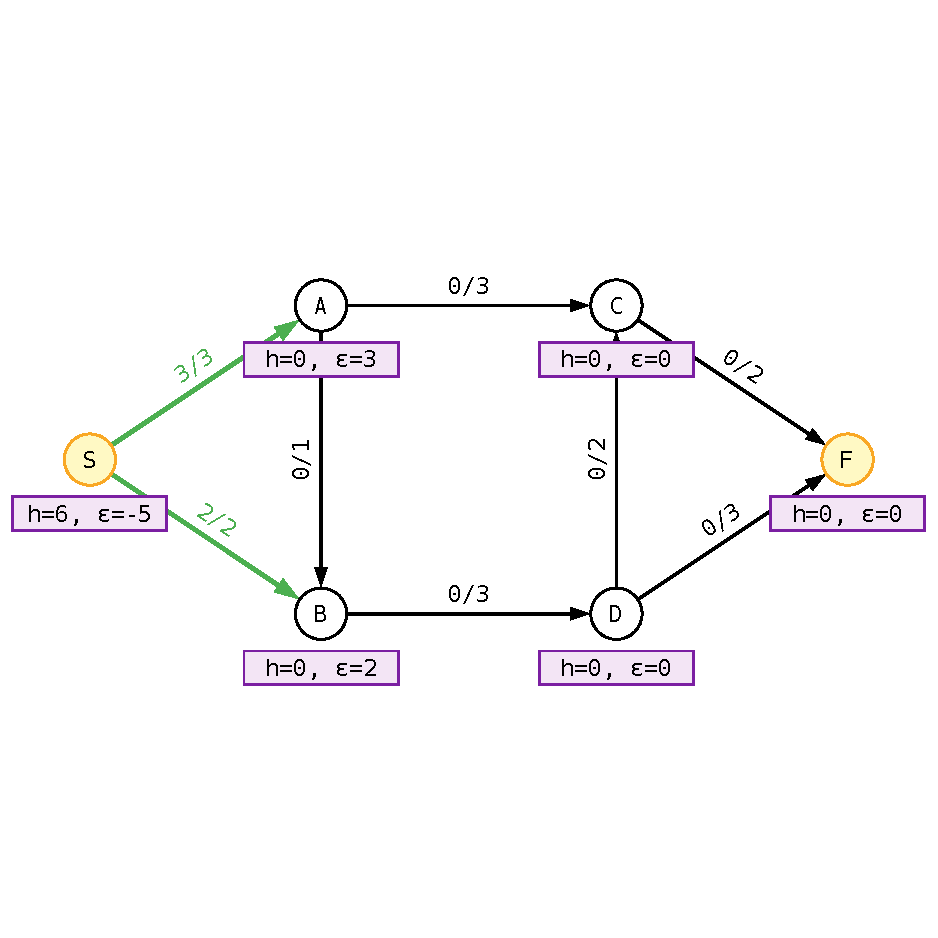
\includegraphics[width=0.46\textwidth]{python/lec11/push_relabel/pr-0.pdf}\\[2pt]{\scriptsize Шаг 0. Инициализация: рёбра из $S$ насыщены}} &
\shortstack{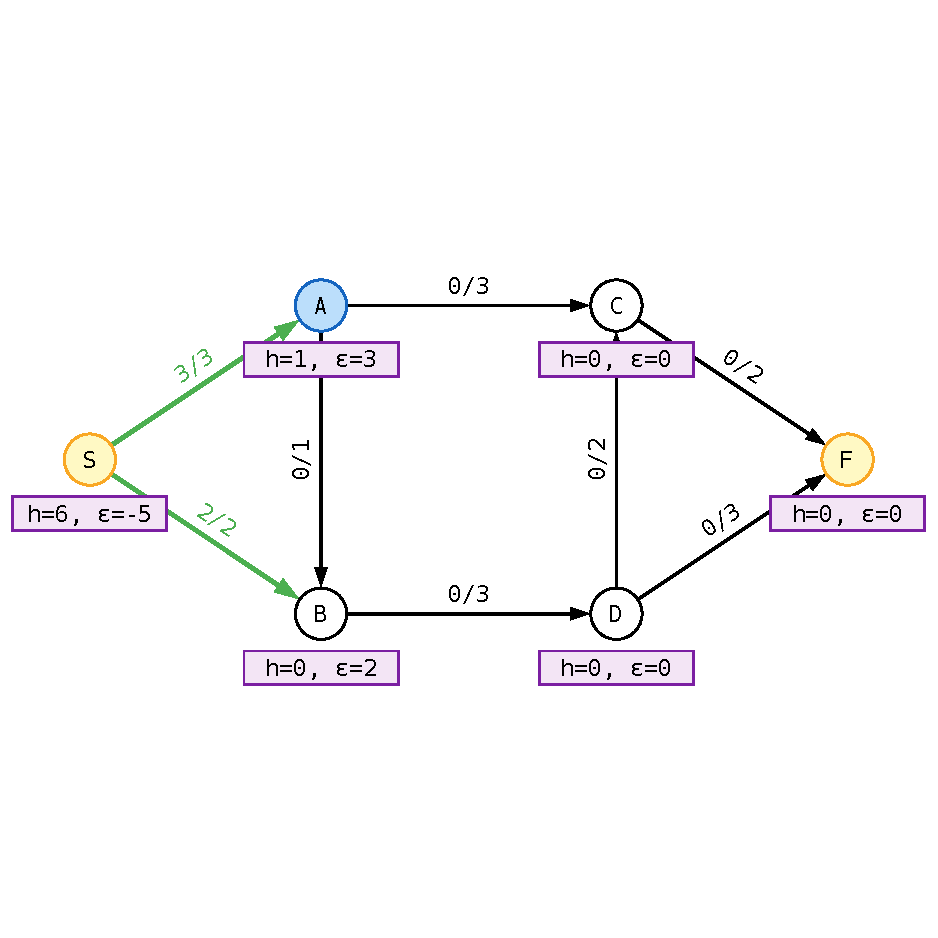
\includegraphics[width=0.46\textwidth]{python/lec11/push_relabel/pr-1.pdf}\\[2pt]{\scriptsize Шаг 1. Lift $A$: $h(A) := 1$}} \\
\end{tabular}\end{center}
\begin{center}\begin{tabular}{cc}
\shortstack{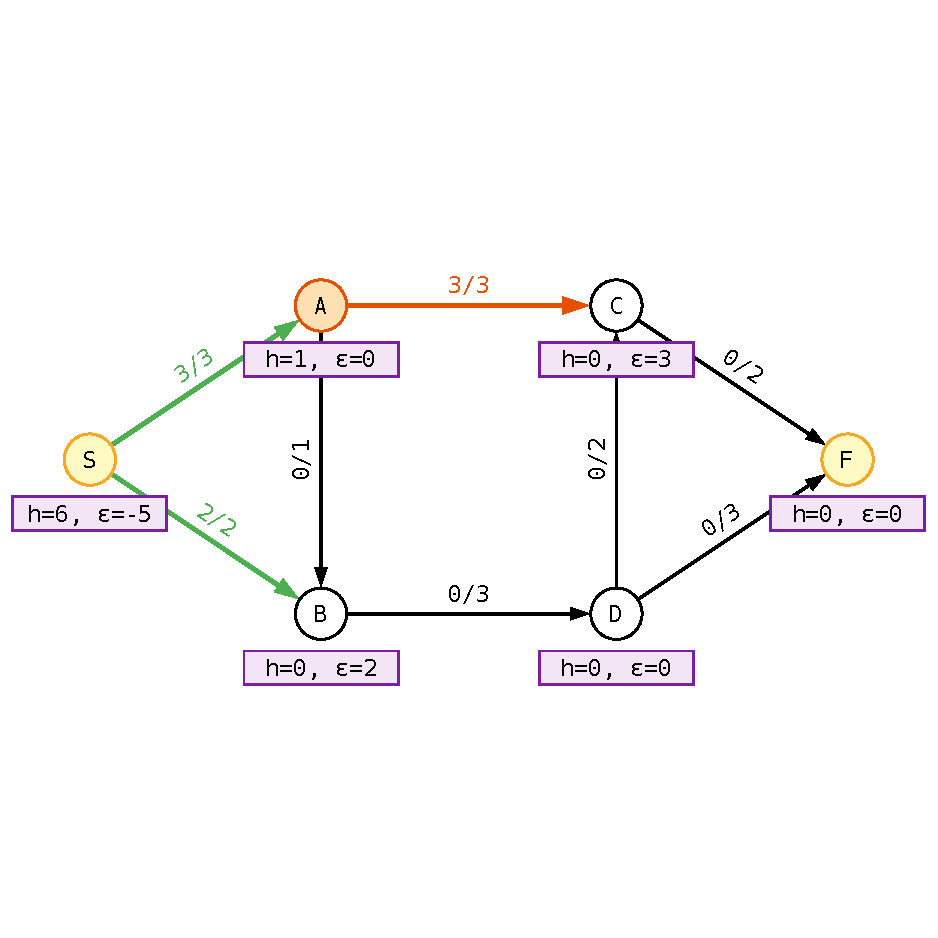
\includegraphics[width=0.46\textwidth]{python/lec11/push_relabel/pr-2.pdf}\\[2pt]{\scriptsize Шаг 2. Push $A \to C$, $\delta = 3$}} &
\shortstack{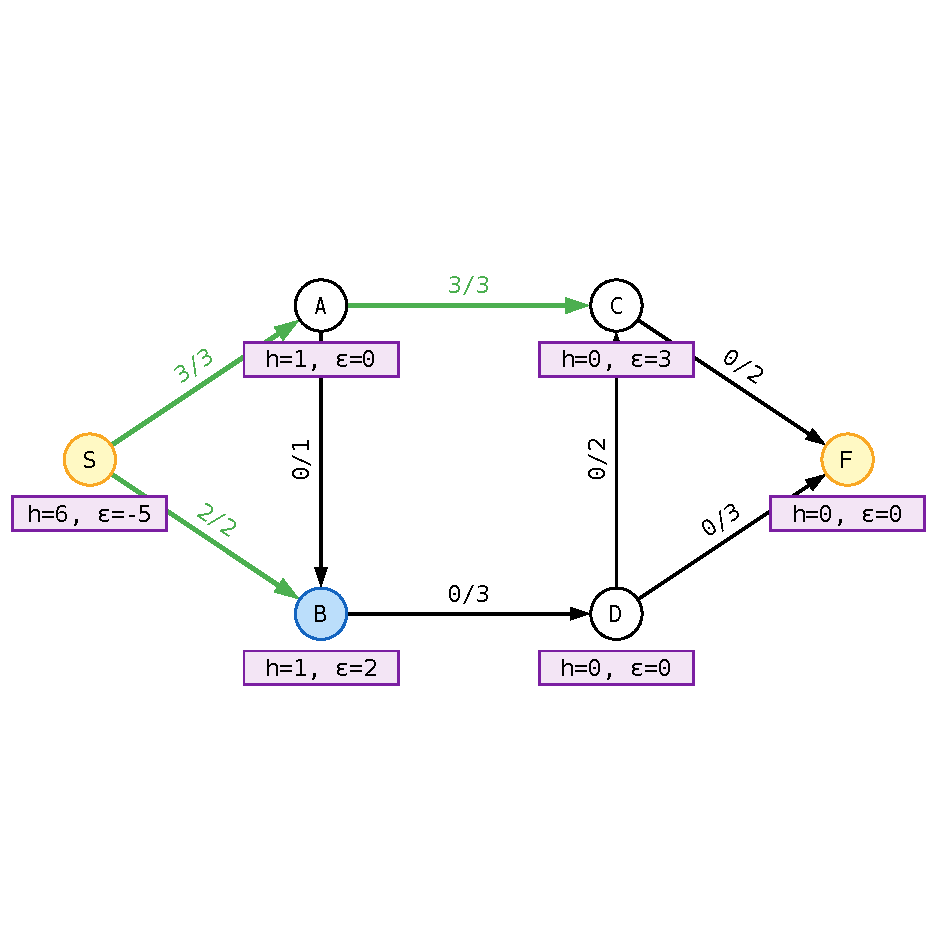
\includegraphics[width=0.46\textwidth]{python/lec11/push_relabel/pr-3.pdf}\\[2pt]{\scriptsize Шаг 3. Lift $B$: $h(B) := 1$}} \\
\end{tabular}\end{center}
\begin{center}\begin{tabular}{cc}
\shortstack{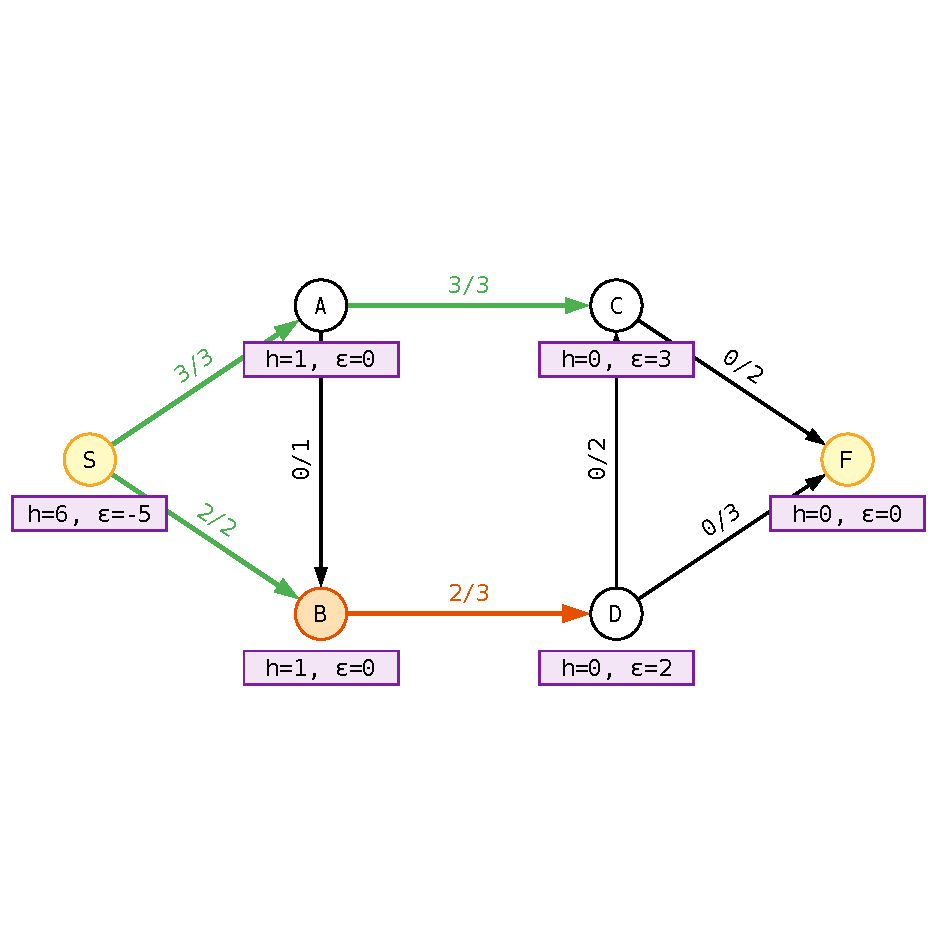
\includegraphics[width=0.46\textwidth]{python/lec11/push_relabel/pr-4.pdf}\\[2pt]{\scriptsize Шаг 4. Push $B \to D$, $\delta = 2$}} &
\shortstack{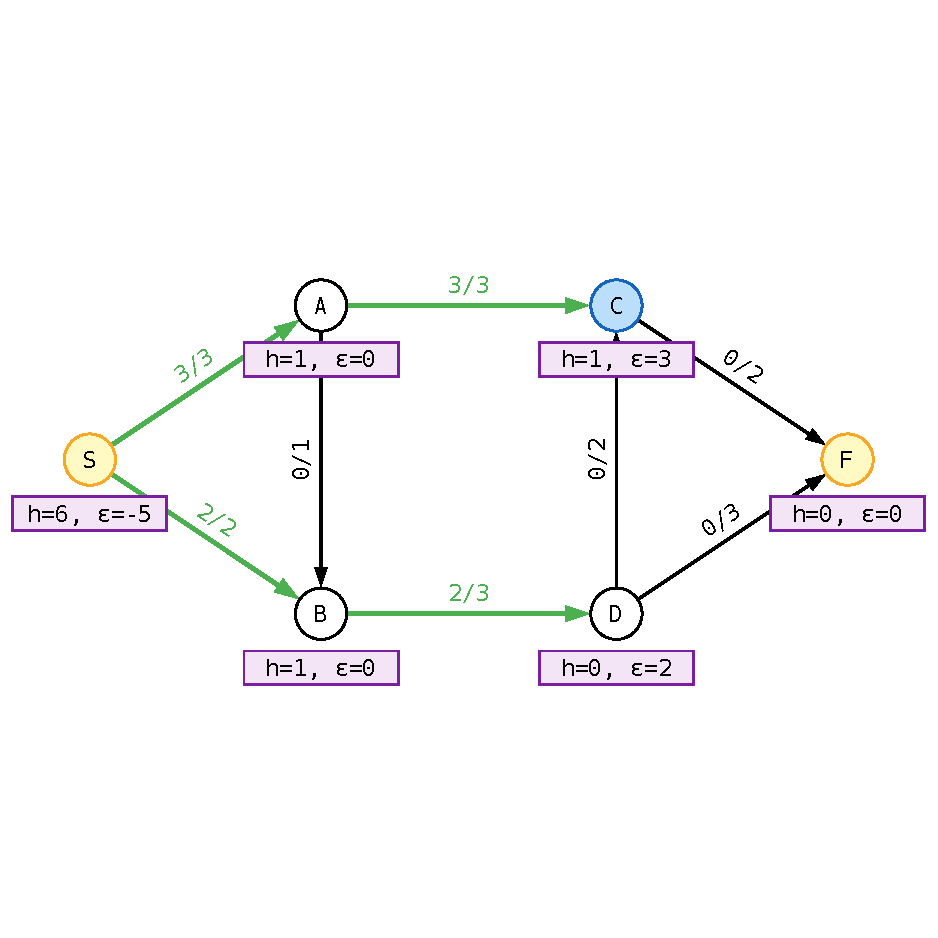
\includegraphics[width=0.46\textwidth]{python/lec11/push_relabel/pr-5.pdf}\\[2pt]{\scriptsize Шаг 5. Lift $C$: $h(C) := 1$}} \\
\end{tabular}\end{center}
\begin{center}\begin{tabular}{cc}
\shortstack{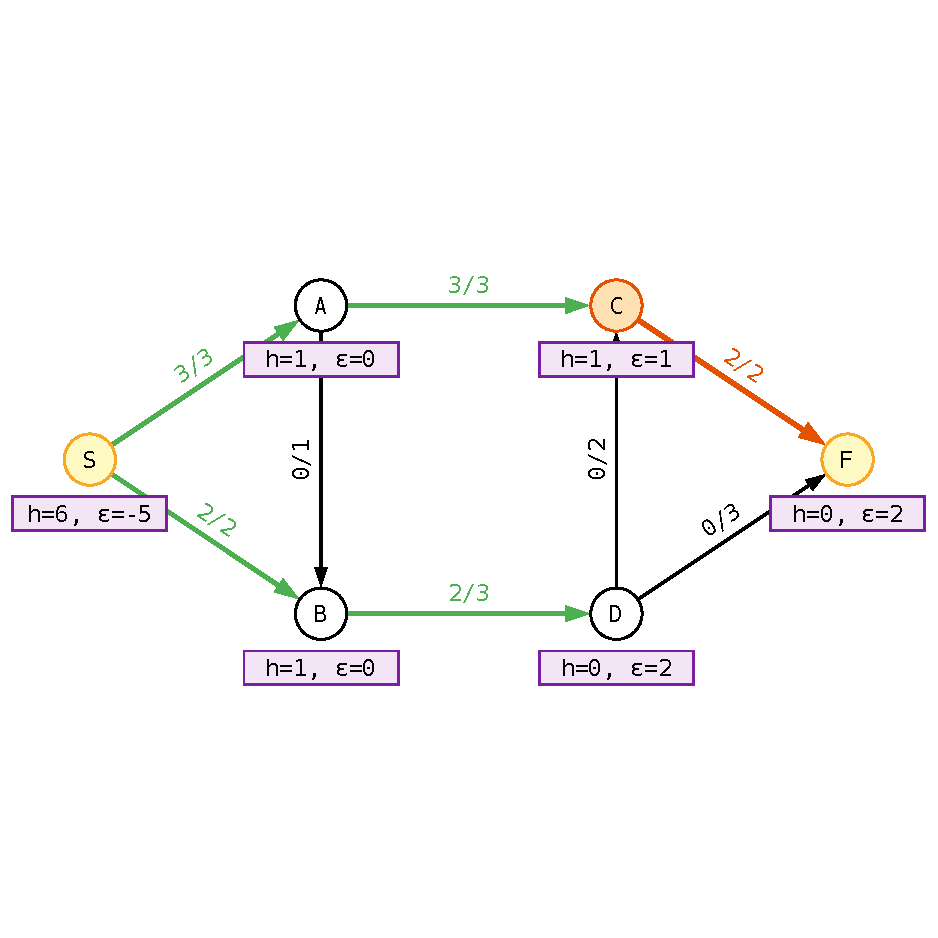
\includegraphics[width=0.46\textwidth]{python/lec11/push_relabel/pr-6.pdf}\\[2pt]{\scriptsize Шаг 6. Push $C \to F$, $\delta = 2$: ребро насыщено}} &
\shortstack{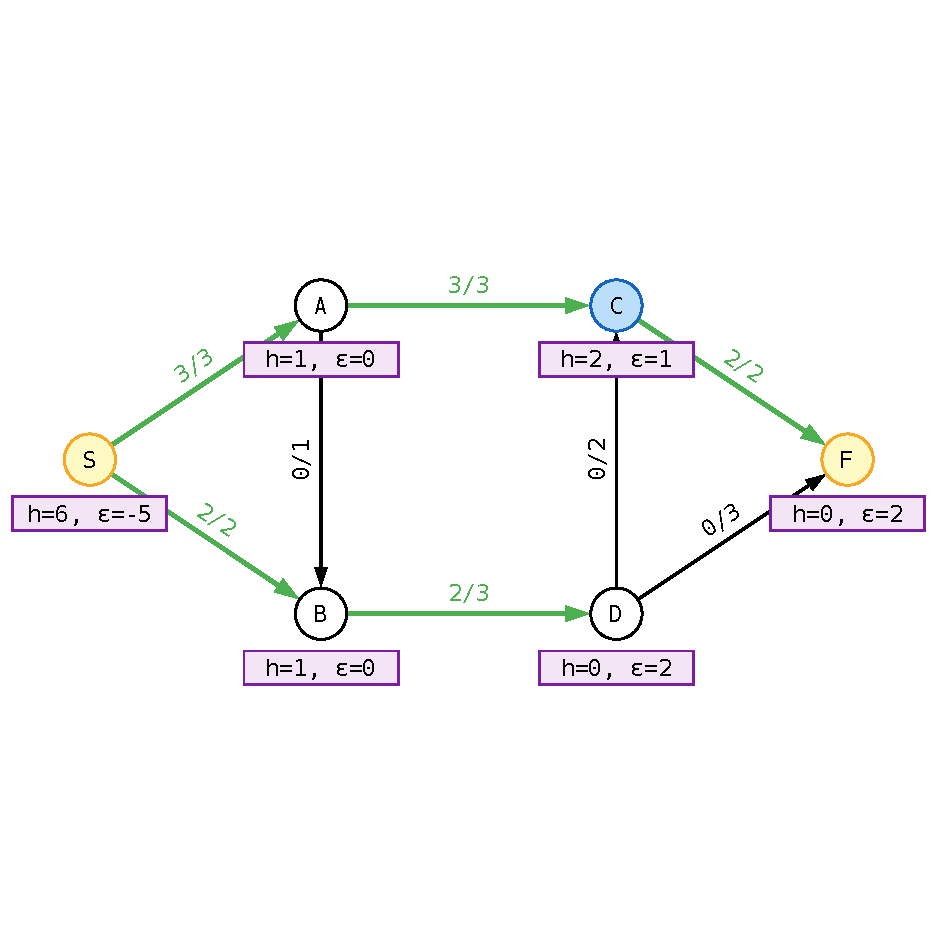
\includegraphics[width=0.46\textwidth]{python/lec11/push_relabel/pr-7.pdf}\\[2pt]{\scriptsize Шаг 7. Lift $C$: $h(C) := 2$ (выше $A$)}} \\
\end{tabular}\end{center}
\begin{center}\begin{tabular}{cc}
\shortstack{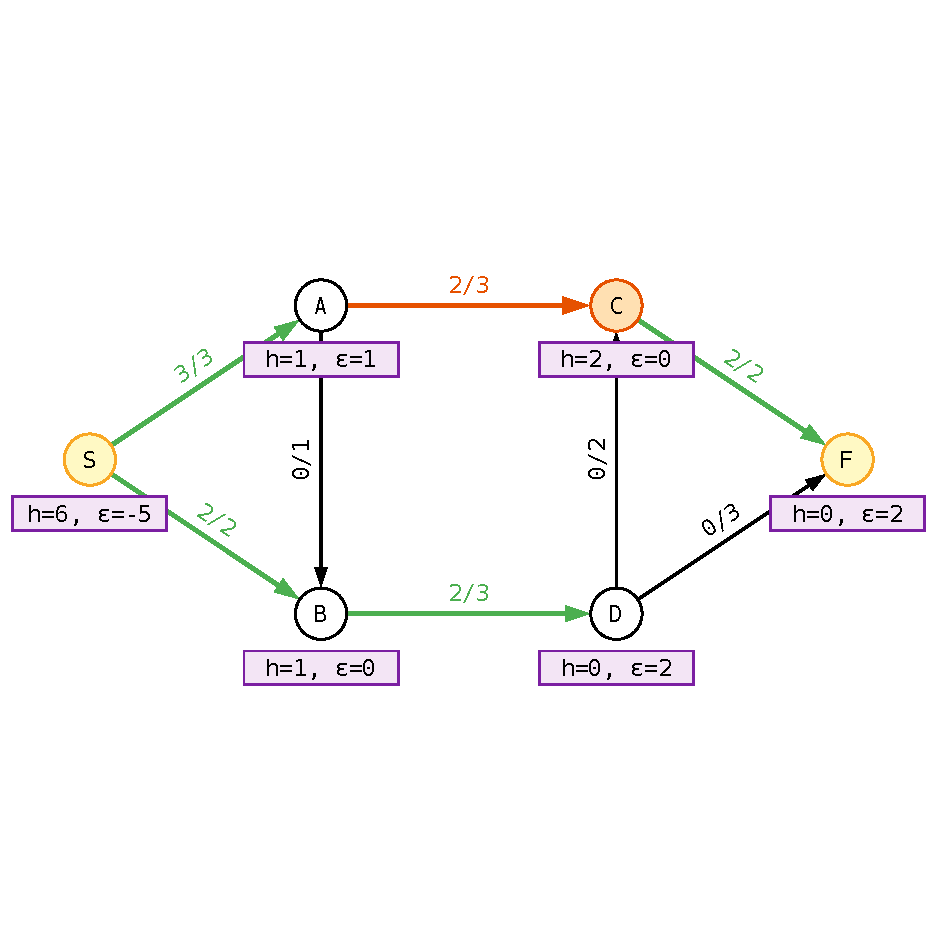
\includegraphics[width=0.46\textwidth]{python/lec11/push_relabel/pr-8.pdf}\\[2pt]{\scriptsize Шаг 8. Push $C \to A$, $\delta = 1$: возврат, $A{\to}C$ стало $2/3$}} &
\shortstack{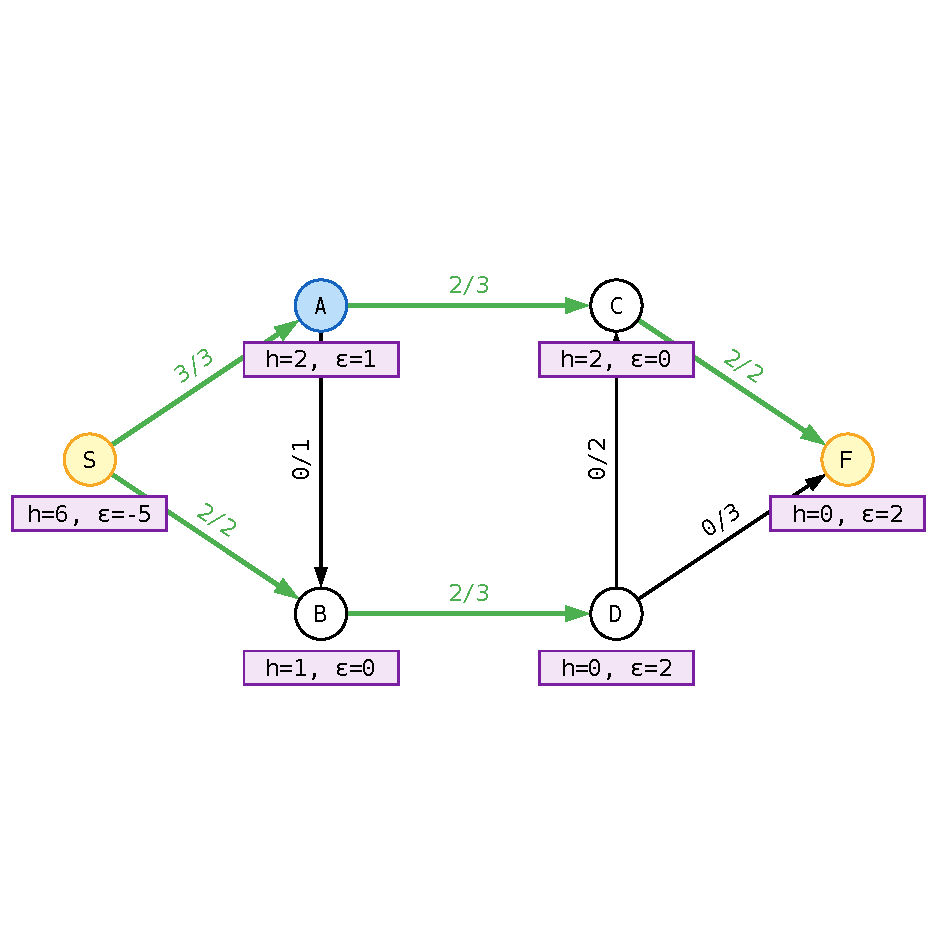
\includegraphics[width=0.46\textwidth]{python/lec11/push_relabel/pr-9.pdf}\\[2pt]{\scriptsize Шаг 9. Lift $A$: $h(A) := 2$}} \\
\end{tabular}\end{center}
\begin{center}\begin{tabular}{cc}
\shortstack{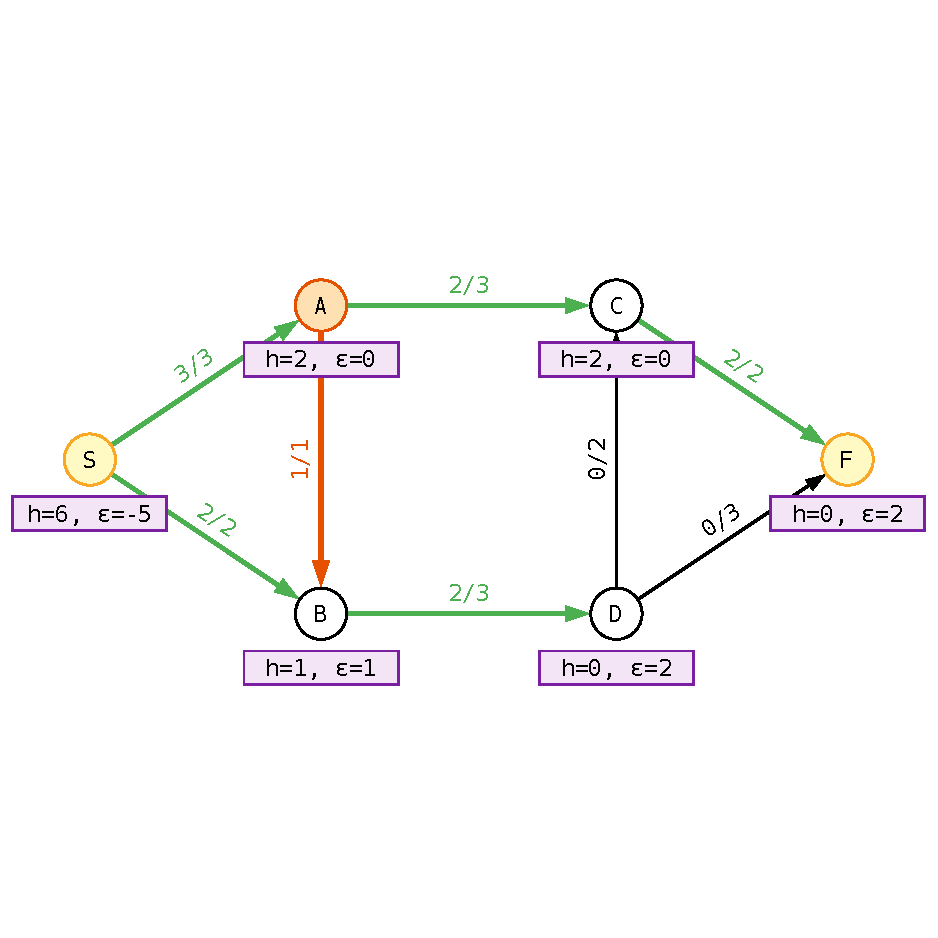
\includegraphics[width=0.46\textwidth]{python/lec11/push_relabel/pr-10.pdf}\\[2pt]{\scriptsize Шаг 10. Push $A \to B$, $\delta = 1$}} &
\shortstack{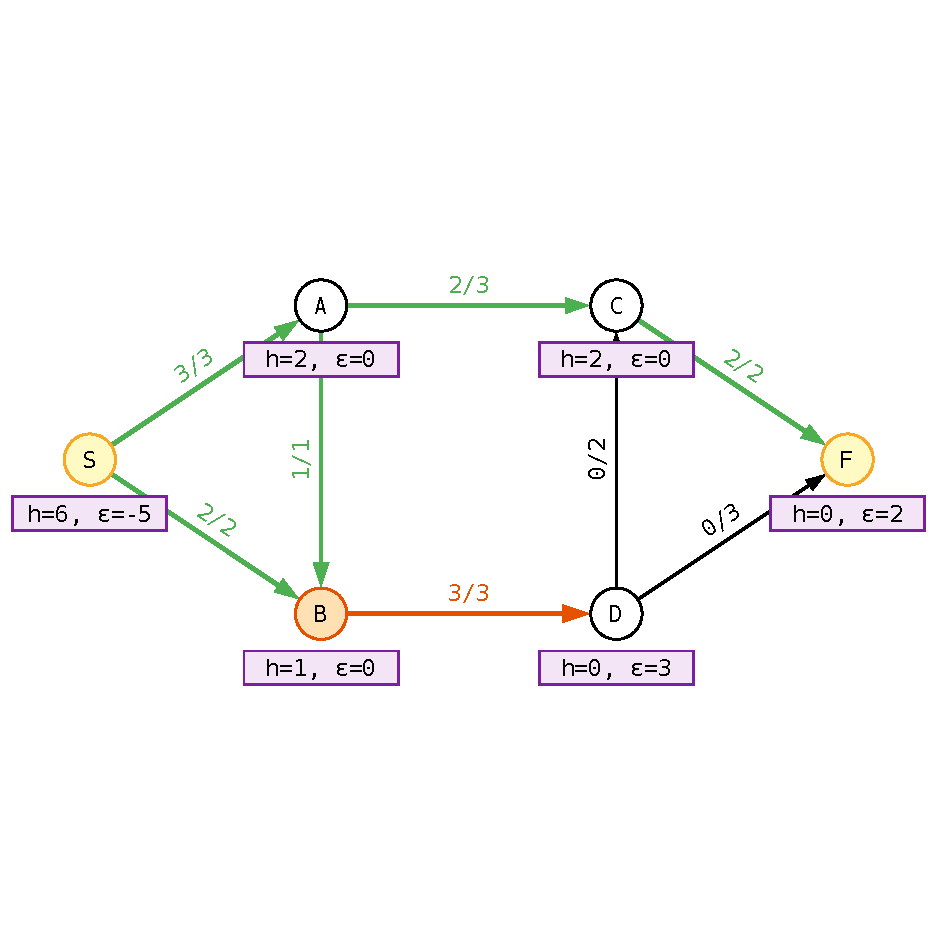
\includegraphics[width=0.46\textwidth]{python/lec11/push_relabel/pr-11.pdf}\\[2pt]{\scriptsize Шаг 11. Push $B \to D$, $\delta = 1$}} \\
\end{tabular}\end{center}
\begin{center}\begin{tabular}{cc}
\shortstack{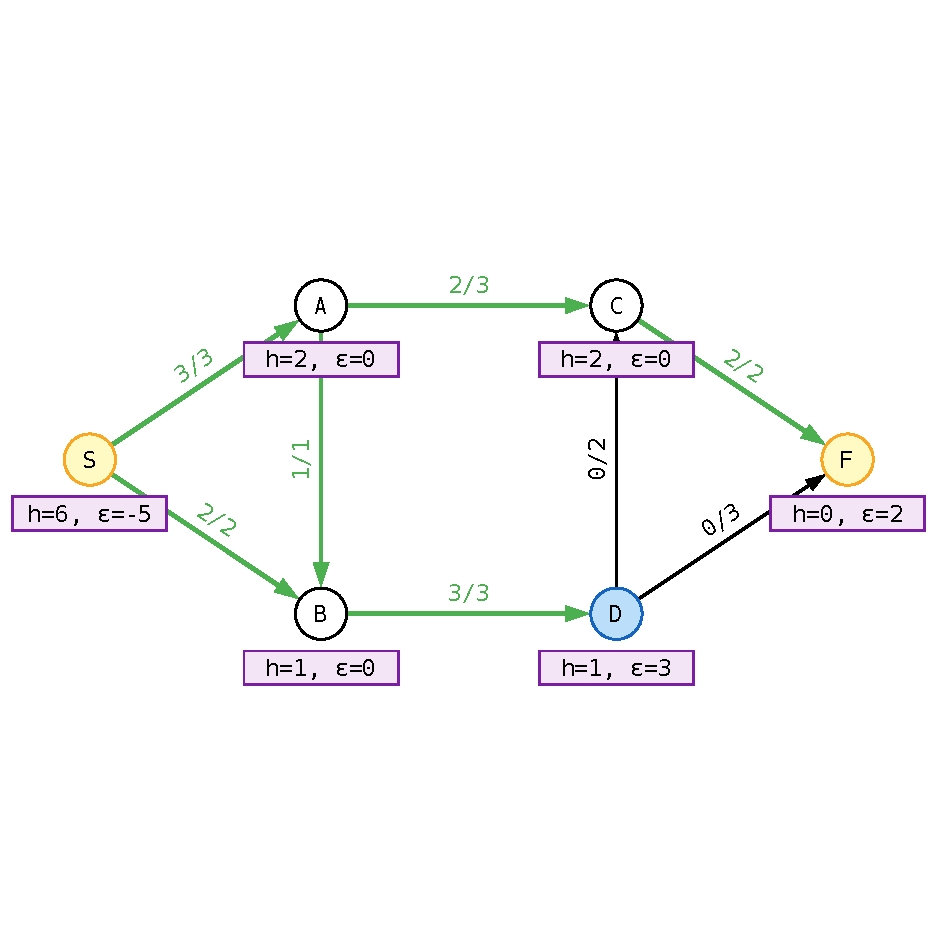
\includegraphics[width=0.46\textwidth]{python/lec11/push_relabel/pr-12.pdf}\\[2pt]{\scriptsize Шаг 12. Lift $D$: $h(D) := 1$}} &
\shortstack{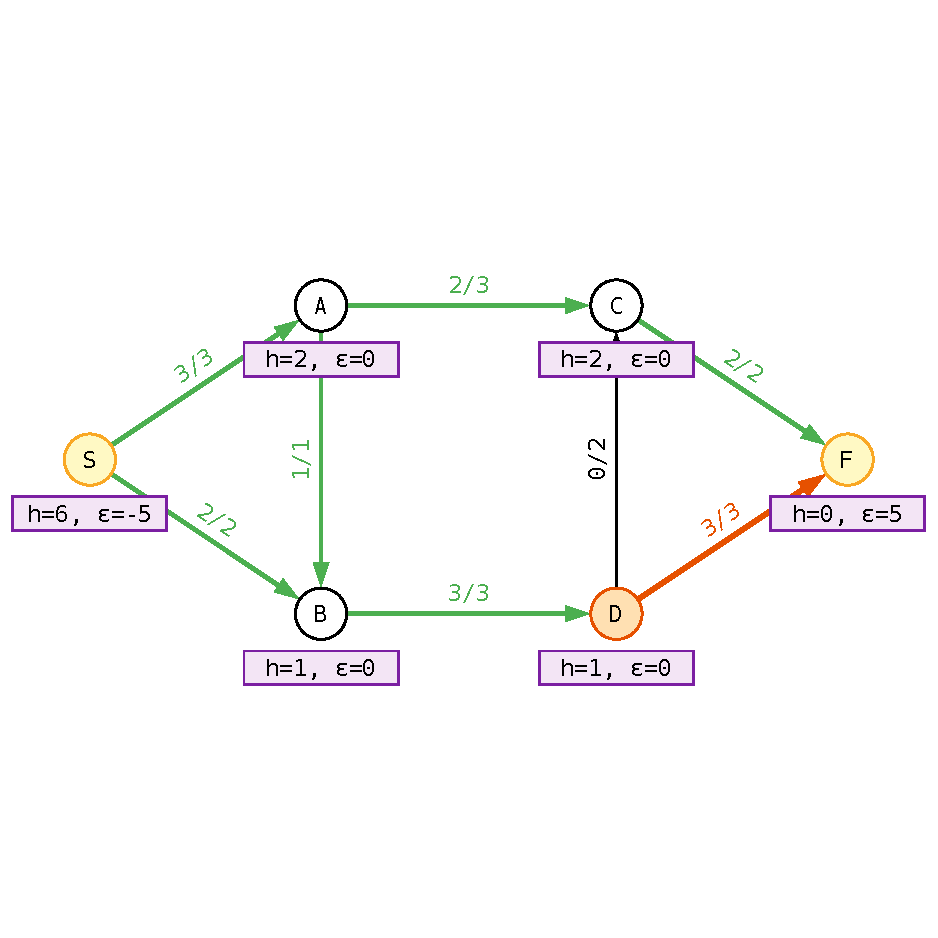
\includegraphics[width=0.46\textwidth]{python/lec11/push_relabel/pr-13.pdf}\\[2pt]{\scriptsize Шаг 13. Push $D \to F$, $\delta = 3$: $|f| = 5$, конец}} \\
\end{tabular}\end{center}
\end{algo}

\medskip
\textbf{Замечание (сумма эксцессов).} В любой момент работы
$\sum_{v \in V} \varepsilon(v) = 0$: каждая единица предпотока на ребре
$uv$ входит в $\varepsilon(v)$ со знаком <<плюс>> и в $\varepsilon(u)$
со знаком <<минус>>, поэтому при суммировании всё сокращается.
В частности, в конце работы $\varepsilon(F) = -\varepsilon(S) = |f|$.

% ===========================================================
%  Хроматика (раскраска графов)
% ===========================================================

\subsection*{Хроматика (раскраска графов)}

\textbf{NB.} Пока рассматриваем \emph{вершинные} раскраски.

\begin{defn}{Правильная раскраска графа}{proper-coloring}
Раскраска графа называется \textbf{правильной}, если любые две смежные вершины окрашены в разные цвета.
\end{defn}

\begin{defn}{Хроматическое число}{chromatic-number}
\textbf{Хроматическое число графа} $\chi(G)$~--- минимальное число цветов, в которые можно правильно раскрасить граф $G$.
\end{defn}

\textbf{Примеры:}
\begin{enumerate}
  \item $|E| = 0 \Rightarrow \chi(G) = 1$: изолированные вершины можно
        красить одним цветом --- конфликтовать нечему.
  \item $|E| > 0 \Rightarrow \chi(G) \geq 2$: у любого ребра концы
        обязаны различаться.
  \item У любого двудольного графа (с рёбрами) $\chi(G) = 2$: красим
        долю $V_1$ первым цветом, долю $V_2$ --- вторым; все рёбра идут
        между долями, конфликтов нет.
  \item $\chi(K_n) = n$: все вершины попарно смежны, поэтому все цвета
        обязаны быть различны (рис.~ниже: $K_4$, $\chi = 4$).
  \item $\chi(C_{2n+1}) = 3$: двух цветов не хватает (нечётный цикл не
        двудолен --- лекция 9), а три цвета есть: чередуем $1, 2$ по
        циклу, последней вершине даём цвет $3$ (рис.~ниже: $C_5$).
        Для чётных циклов $\chi(C_{2n}) = 2$.
\end{enumerate}

\grfig[0.4]{figures/p25-example-2.pdf}{Хром. число: $K_4$, $\chi = 4$ --- все цвета различны}
\grfig[0.4]{figures/p25-example-3.pdf}{Хром. число: $C_5$, $\chi = 3$ --- чередование $1,2$ и третий цвет}

\begin{defn}{Клика}{clique}
\textbf{Клика}~--- максимальный полный подграф графа $G$.
\end{defn}

\begin{lemma}{О клике}{clique-chromatic}
Если $K_n$~--- наибольшая клика в $G$, то $\chi(G) \geq n$.
\end{lemma}

\begin{proof}
Любая правильная раскраска $G$ является правильной и на подграфе $K_n$.
Но в $K_n$ все $n$ вершин попарно смежны, поэтому уже им требуется $n$
различных цветов: $\chi(G) \ge \chi(K_n) = n$.
\end{proof}


% ===========================================================
%  Лекция 12. Хроматический многочлен
% ===========================================================

\chapter{Лекция 12. Хроматический многочлен}

\begin{defn}{Хроматический многочлен}{chromatic-polynomial}
Пусть $G(V, E)$~--- граф. \textbf{Хроматический многочлен} графа $G$:
\[
  P_G\colon \mathbb{N}_0 \to \mathbb{N}_0, \qquad
  P_G(t) = a_1 t + a_2 t^2 + \ldots + a_n t^n,
\]
т.\,е.\ это многочлен, значение которого $P_G(k)$ равно числу правильных раскрасок $G$ в $k$ цветов ($\forall\, k \in \mathbb{N}_0$).
\end{defn}

\textbf{Примеры:}
\begin{enumerate}
  \item Пустой граф ($n$ изолированных вершин): $P_G(t) = t^n$ ---
        каждая вершина красится независимо любым из $t$ цветов.
  \item $K_n$: $P_{K_n}(t) = t(t-1)(t-2)\cdots(t-(n-1))$ --- красим
        вершины по очереди, каждая обязана отличаться от всех
        предыдущих.
  \item Дерево $T_n$ ($n$ вершин): $P_{T_n}(t) = t(t-1)^{n-1}$ ---
        красим от корня: корень $t$ способами, каждую следующую вершину
        (по мере удаления от корня) --- $t - 1$ способами, лишь бы она
        отличалась от единственного уже покрашенного соседа (родителя).
\end{enumerate}

Иллюстрация на двух деревьях с $n = 4$ (показана одна из правильных
раскрасок в 2 цвета):

\grfig[0.4]{figures/p26-example-1.pdf}{Путь $P_4$: $P(t) = t(t-1)^3$; в 2 цвета --- ровно 2 раскраски}
\grfig[0.4]{figures/p26-example-2.pdf}{Звезда: тоже $P(t) = t(t-1)^3$ --- дерево с тем же $n$}

Заметим: путь и звезда --- \emph{разные} графы с \emph{одинаковым}
хроматическим многочленом (см.~свойство 4 ниже).

\medskip
\textbf{Тривиальные свойства} (с обоснованиями):
\begin{enumerate}[label=\arabic*)]
  \setcounter{enumi}{-1}
  \item $P_G$~--- многочлен. \textit{Почему:} сгруппируем раскраски по
        числу $i$ реально использованных цветов: если $\alpha_i$ ---
        число разбиений $V$ на $i$ непустых независимых (попарно
        несмежных внутри) множеств, то
        $P_G(t) = \sum_{i} \alpha_i \cdot t(t-1)\cdots(t-i+1)$ ---
        выбираем, какие именно $i$ из $t$ цветов достанутся классам
        разбиения. Это конечная сумма многочленов.
  \item $\deg(P_G) = |V|$. \textit{Почему:} старшее слагаемое в сумме
        выше отвечает $i = n$ (все вершины разных цветов, $\alpha_n = 1$)
        и равно $t(t-1)\cdots(t-n+1)$ --- многочлен степени $n$.
  \item $P_G(0) = 0$ для $\forall\, G$ т.\,ч.\ $|V| > 0$:
        в $0$ цветов нельзя раскрасить даже одну вершину.
  \item $P_G(t) = t^k \cdot g(t)$, где $g(0) \neq 0$, $k$~--- число
        компонент связности графа $G$. \textit{Почему:} компоненты
        красятся независимо, поэтому $P_G$ --- произведение многочленов
        компонент, и каждый сомножитель делится на $t$ ровно один раз.
  \item $G$ по $P_G$ не восстанавливается однозначно.
        \textit{Контрпример:} все деревья на $n$ вершинах имеют один и
        тот же многочлен $t(t-1)^{n-1}$, но при $n \ge 4$ дерево не
        единственно (путь $P_4$ и звезда на рисунках выше).
  \item $a_n = 1$ (старший коэффициент) --- см.~обоснование свойства 1.
  \item $\forall\, 1 \leq i \leq n-1\colon a_i \cdot a_{i+1} \leq 0$
        (знакочередование). \textit{Идея:} индукция по числу рёбер с
        теоремой о редукции в форме
        $P_G = P_{G \setminus e} - P_{G/e}$: у $P_{G\setminus e}$
        и $P_{G/e}$ знаки чередуются по предположению, степени
        отличаются на $1$, и при вычитании чередование сохраняется.
  \item $|E_G| > 0 \;\Rightarrow\; P_G(1) = 0$: при одном цвете концы
        любого ребра совпадут по цвету. Более точно,
        $P_G(t) = (t-1)^d \cdot g(t)$, где $g(1) \neq 0$, $d$~--- число
        блоков (компонент вершинной двусвязности) в $G$.
\end{enumerate}

\subsection*{Как найти $P_G$?}

\begin{statement}{Теорема о редукции}{reduction-theorem}
Пусть $G(V, E)$, и $u, v \in V$~--- не смежные вершины. Тогда:
\[
  P_G(t) = P_{G \vee uv}(t) + P_{G * uv}(t),
\]
где $G \vee uv$~--- граф с добавленным ребром $uv$ (приближаем к полному), а $G * uv$~--- граф со стянутыми вершинами $u$ и $v$.
\end{statement}

\begin{proof}
Разобьём все правильные раскраски $G$ в $t$ цветов на два класса по
тому, как покрашены $u$ и $v$ (они не смежны, поэтому возможно и то,
и другое):
\begin{itemize}
  \item \textbf{цвета $u$ и $v$ различны} --- такие раскраски взаимно
        однозначно соответствуют правильным раскраскам графа
        $G \vee uv$: добавленное ребро $uv$ как раз и требует
        различия цветов, остальные ограничения совпадают;
  \item \textbf{цвета $u$ и $v$ совпадают} --- такие раскраски взаимно
        однозначно соответствуют правильным раскраскам графа $G * uv$:
        склеенная вершина получает этот общий цвет, и её смежности ---
        объединение смежностей $u$ и $v$.
\end{itemize}
Классы не пересекаются и исчерпывают все раскраски, поэтому
$P_G = P_{G \vee uv} + P_{G * uv}$.
\end{proof}

Иллюстрация: $u$ и $v$ не смежны в $G$; слева направо --- $G$,
$G \vee uv$ (зелёное ребро добавлено), $G * uv$ (вершины склеены):

\begin{center}\begin{tabular}{ccc}
\shortstack{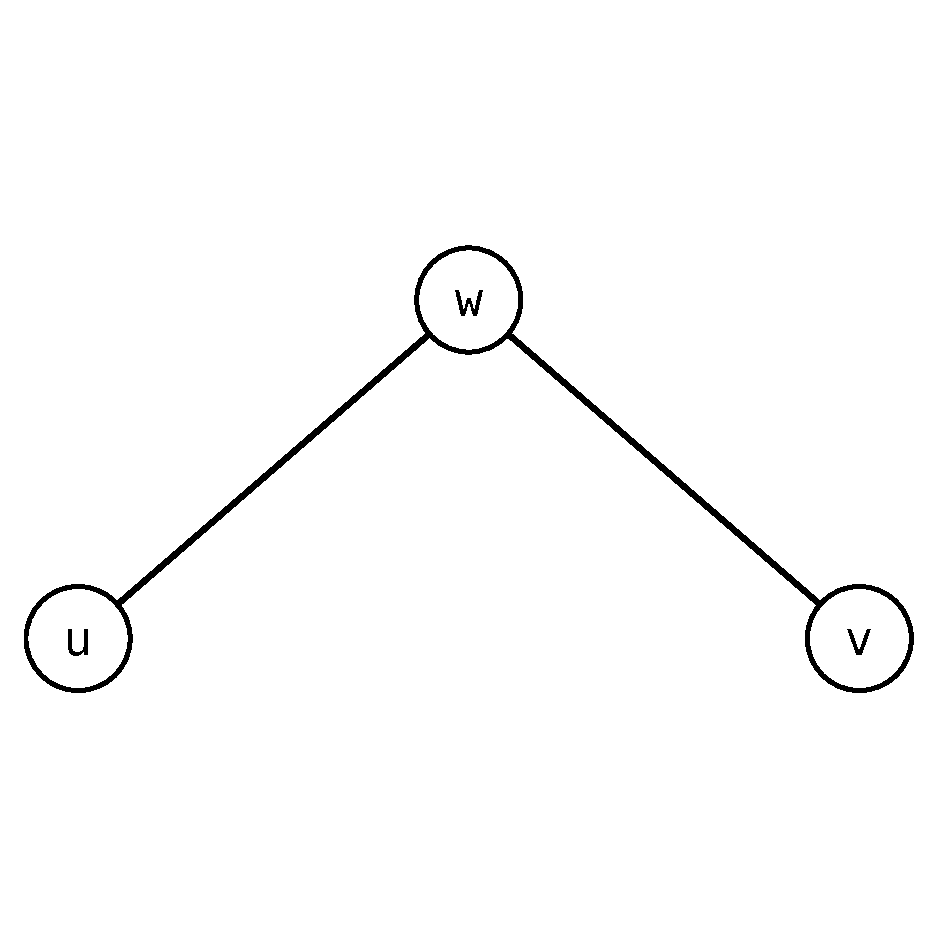
\includegraphics[width=0.26\textwidth]{figures/p26-red-0.pdf}\\[2pt]{\scriptsize $G$: путь $u$--$w$--$v$}} &
\shortstack{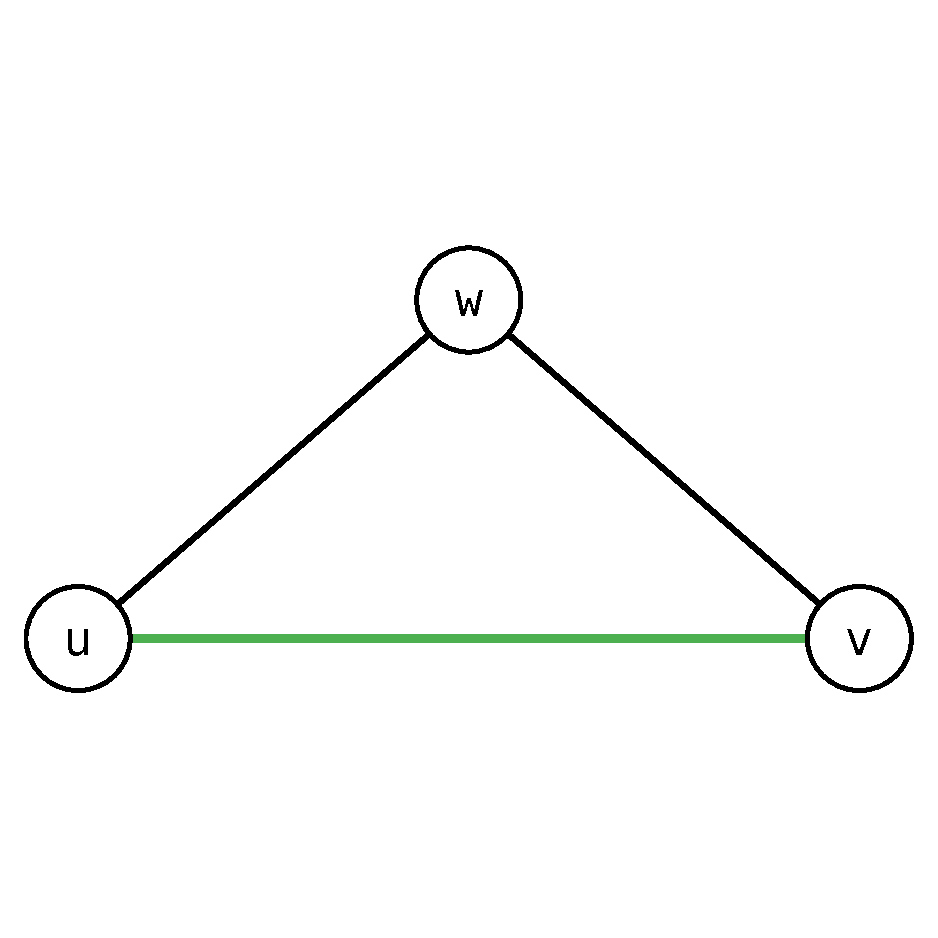
\includegraphics[width=0.26\textwidth]{figures/p26-red-1.pdf}\\[2pt]{\scriptsize $G \vee uv$: треугольник}} &
\shortstack{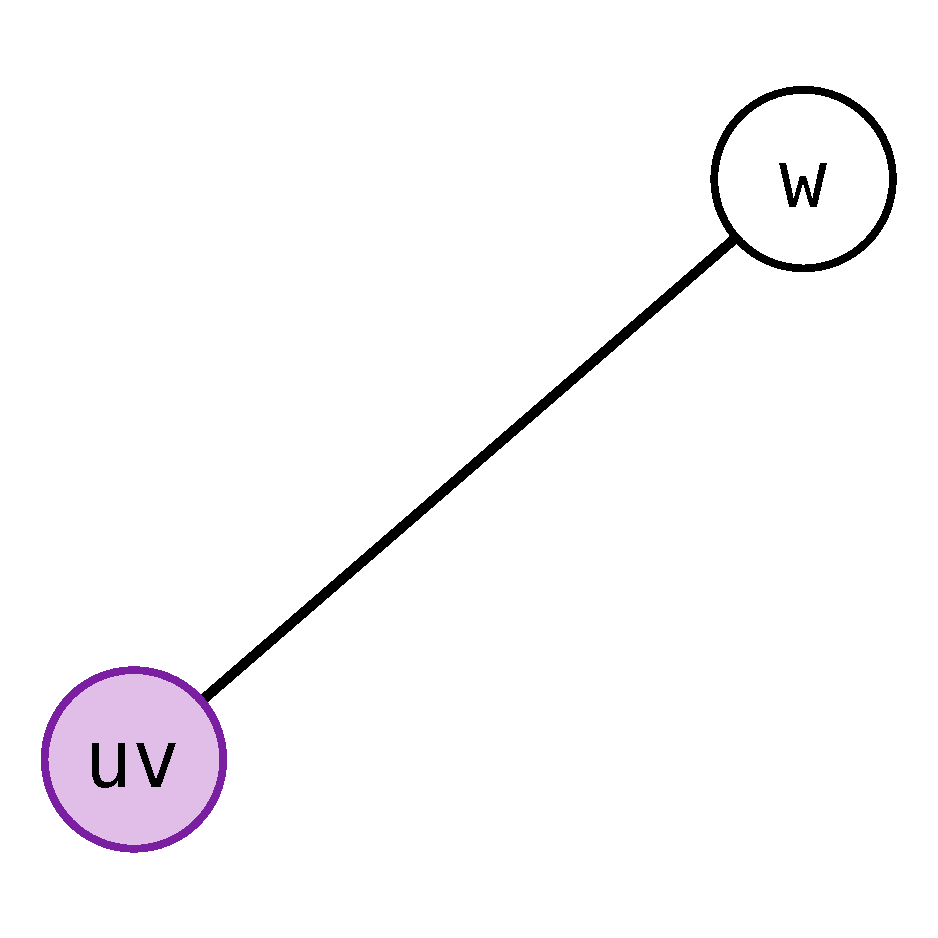
\includegraphics[width=0.26\textwidth]{figures/p26-red-2.pdf}\\[2pt]{\scriptsize $G * uv$: ребро}} \\
\end{tabular}\end{center}

\noindent\textbf{Мини-пример} (проверка теоремы). Для пути
$G = u$--$w$--$v$ на рисунке: $G \vee uv = K_3$, $G * uv = K_2$,
\[
  P_{G \vee uv} + P_{G * uv} = t(t-1)(t-2) + t(t-1) = t(t-1)^2
\]
--- в точности $P_{T_3}(t) = t(t-1)^2$ по формуле для дерева. $\checkmark$

\medskip
\textbf{Следствие.} Если $\exists\, e = uv$ (смежные), то:
\[
  P_G(t) = P_{G \setminus e}(t) - P_{G * uv}(t).
\]
\textit{Почему:} применим теорему к графу $G \setminus e$ (в нём $u, v$
уже не смежны): $P_{G \setminus e} = P_{(G\setminus e) \vee uv} +
P_{(G \setminus e) * uv} = P_G + P_{G * uv}$, и перенесём слагаемое.

\medskip
\textbf{Пример:} Цикл $C_n$:
\[
  P_{C_n}(t) = (t-1)^n + (-1)^n (t-1).
\]

\begin{proof}
Воспользуемся теоремой об удалении и стягивании: для любого ребра $e=uv$
\[
  P_G(t) = P_{G\setminus e}(t) - P_{G/e}(t),
\]
где $G\setminus e$ --- граф с удалённым ребром, а $G/e$ --- граф со
стянутым ребром (вершины $u$ и $v$ отождествлены). Понадобится также
хроматический многочлен простого пути (дерева) на $n$ вершинах:
$P_{T_n}(t)=t(t-1)^{n-1}$ (первую вершину красим $t$ способами, каждую
следующую --- $t-1$ способами, лишь бы она отличалась от предыдущей).

\textbf{База ($n=3$).} $C_3=K_3$, поэтому $P_{C_3}(t)=t(t-1)(t-2)$.
Проверим формулу:
\[
  (t-1)^3+(-1)^3(t-1)=(t-1)\bigl[(t-1)^2-1\bigr]=(t-1)(t^2-2t)=t(t-1)(t-2).
\]

\textbf{Переход.} Возьмём в цикле $C_n$ произвольное ребро $e=uv$. Его удаление
размыкает цикл в путь: $C_n\setminus e=T_n$, поэтому
$P_{C_n\setminus e}(t)=t(t-1)^{n-1}$. Стягивание ребра $e$ склеивает $u$ и $v$
и превращает цикл из $n$ вершин в цикл из $n-1$ вершины: $C_n/e=C_{n-1}$.
По теореме об удалении и стягивании
\[
  P_{C_n}(t)=t(t-1)^{n-1}-P_{C_{n-1}}(t).
\]
Подставляя предположение индукции
$P_{C_{n-1}}(t)=(t-1)^{n-1}+(-1)^{n-1}(t-1)$, получаем
\[
  P_{C_n}(t)=t(t-1)^{n-1}-(t-1)^{n-1}-(-1)^{n-1}(t-1)
           =(t-1)^{n-1}(t-1)+(-1)^{n}(t-1),
\]
то есть $P_{C_n}(t)=(t-1)^n+(-1)^n(t-1)$, что и требовалось.
\end{proof}

\subsection*{Теорема о разделяющей клике}

\begin{lemma}{Лемма 1 (висячая вершина)}{separating-clique-1}
Если в графе $G$ есть висячая вершина $u$, соединённая с подграфом $G_1$, то:
\[
  P_G(t) = P_{G_1}(t) \cdot (t-1).
\]
\grfig{figures/p27-lemma1.pdf}{Лемма 1: висячая вершина -> P\_G = P\_\{G1\}.(t-1)}
\end{lemma}

\begin{proof}
Сначала правильно красим $G_1$ --- $P_{G_1}(t)$ способами. У вершины $u$
ровно один сосед, и какой бы цвет он ни получил, для $u$ остаётся
$t - 1$ допустимых цветов; выбор независим от остального. По правилу
произведения $P_G(t) = P_{G_1}(t)(t-1)$.
\end{proof}

\begin{lemma}{Лемма 2 (дерево $T_{n+1}$)}{separating-clique-2}
Если к подграфу $G_1$ присоединено дерево $T_{n+1}$ (через одну вершину), то:
\[
  P_G(t) = P_{G_1}(t) \cdot (t-1)^n.
\]
\grfig{figures/p27-lemma2.pdf}{Лемма 2: дерево T\_\{n+1\} -> P\_G = P\_\{G1\}.(t-1)\^{}n}
\end{lemma}

\begin{proof}
Дерево $T_{n+1}$ имеет $n + 1$ вершину (одна из них --- общая с $G_1$)
и $n$ рёбер. Присоединяем его вершины по одной, начиная от общей вершины
и удаляясь по дереву: каждая новая вершина --- висячая относительно уже
покрашенной части, и по лемме~1 даёт множитель $(t-1)$. Всего $n$ новых
вершин: $P_G = P_{G_1} \cdot (t-1)^n$.
\end{proof}

\begin{lemma}{Лемма 3 (вершина при ребре)}{separating-clique-3}
Если вершина $u$ присоединена к $G_1$ рёбрами к \emph{обоим концам}
некоторого ребра $vw \in G_1$ (т.\,е.\ через клику $K_2$), то:
\[
  P_G(t) = P_{G_1}(t) \cdot (t-2).
\]
\grfig{figures/p27-lemma3.pdf}{Лемма 3: вершина при ребре -> P\_G = P\_\{G1\}.(t-2)}
\end{lemma}

\begin{proof}
В любой правильной раскраске $G_1$ концы ребра $vw$ покрашены в
\emph{два различных} цвета. Вершине $u$ запрещены ровно эти два цвета,
остаётся $t - 2$ вариантов --- независимо от того, какая именно
раскраска $G_1$ выбрана.
\end{proof}

\begin{lemma}{Лемма 4 (вершина при $K_n$)}{separating-clique-4}
Если вершина $u$ с $\deg u = n$ присоединена к подграфу $G_1$ через $K_n$
(все $n$ соседей $u$ попарно смежны в $G_1$), то:
\[
  P_G(t) = P_{G_1}(t) \cdot (t - n).
\]
\grfig{figures/p27-lemma4.pdf}{Лемма 4: вершина при K\_n -> P\_G = P\_\{G1\}.(t-n)}
\end{lemma}

\begin{proof}
Соседи $u$ образуют клику, поэтому в любой правильной раскраске $G_1$
они покрашены в $n$ \emph{попарно различных} цветов. Для $u$ запрещены
ровно $n$ цветов --- остаётся $t - n$ вариантов. Леммы 1 и 3 ---
частные случаи при $n = 1$ и $n = 2$.
\end{proof}

\begin{lemma}{Лемма 5 (комбинация подвесок)}{separating-clique-5}
Если к $G_1$ присоединены висячая вершина и вершина при ребре
(как на рисунке), множители перемножаются:
\[
  P_G(t) = P_{G_1}(t) \cdot (t-1)(t-2).
\]
\grfig{figures/p27-lemma5.pdf}{Лемма 5: висячая вершина + вершина при ребре}
\end{lemma}

\begin{proof}
Применяем леммы по очереди: сначала к $G' = G$ без висячей вершины
$5$ --- по лемме~3 (вершина $6$ при ребре $3$--$4$) имеем
$P_{G'} = P_{G_1}(t-2)$; затем возвращаем висячую вершину $5$ --- по
лемме~1 получаем $P_G = P_{G'}(t-1) = P_{G_1}(t-1)(t-2)$. Порядок
применения не важен: каждая подвеска даёт свой множитель независимо.
\end{proof}

\begin{lemma}{Лемма 6 (общая, разделяющая $K_n$)}{separating-clique-6}
Если граф $G$ разделяется кликой $K_n$ на подграфы $G_1$ и $G_2$
(т.\,е.\ $G = G_1 \cup G_2$, $G_1 \cap G_2 = K_n$), то:
\[
  P_G(t) = \frac{P_{G_1}(t) \cdot P_{G_2}(t)}{P_{K_n}(t)}.
\]
\grfig{figures/p27-lemma6.pdf}{Лемма 6: общая, K\_n -> P\_G = P\_\{G1\}.P\_\{G2\}/P\_\{K\_n\}}
\end{lemma}

\begin{proof}
Ключевое наблюдение: \emph{число продолжений} фиксированной правильной
раскраски клики $K_n$ до правильной раскраски всего $G_1$ не зависит
от того, какая именно раскраска клики выбрана. Действительно, любые две
правильные раскраски $K_n$ ($n$ попарно различных цветов) переводятся
друг в друга перестановкой цветов, а перестановка цветов --- биекция
на множестве продолжений. Поэтому продолжений ровно
$P_{G_1}(t) / P_{K_n}(t)$ (всего раскрасок $G_1$, делённое на число
раскрасок клики); аналогично для $G_2$.

Раскраска $G$ --- это раскраска клики ($P_{K_n}(t)$ способов) плюс
независимые продолжения на $G_1$ и на $G_2$ (общих вершин вне клики
нет, рёбер между $G_1 \setminus K_n$ и $G_2 \setminus K_n$ нет):
\[
  P_G = P_{K_n} \cdot \frac{P_{G_1}}{P_{K_n}} \cdot \frac{P_{G_2}}{P_{K_n}}
      = \frac{P_{G_1} \cdot P_{G_2}}{P_{K_n}}.
\]
Леммы 1--5 --- частные случаи (например, лемма 4: $G_2 = K_{n+1}$,
$P_{G_2}/P_{K_n} = t - n$).
\end{proof}

\subsection*{Рёберная раскраска}

\begin{defn}{Правильная рёберная раскраска}{proper-edge-coloring}
Рёберная раскраска графа называется \textbf{правильной}, если $\forall\, e_1, e_2 \in E$, имеющие общую вершину, окрашены в разные цвета.
\end{defn}

\begin{defn}{Хроматически двойственный граф}{chromatic-dual}
Пусть $G(V, E)$. \textbf{Хроматически двойственный} граф $G_\chi(V_\chi, E_\chi)$ строится так:
\begin{enumerate}
  \item $V_\chi = E$ \quad (вершины $G_\chi$~--- это рёбра $G$);
  \item $\hat{u}, \hat{v} \in V_\chi$: $\exists\, \hat{e} = \hat{u}\hat{v} \;\Leftrightarrow\;$ рёбра $u, v \in E$ имеют общую вершину в $G$.
\end{enumerate}
Правильные \emph{рёберные} раскраски $G$ --- это в точности правильные
\emph{вершинные} раскраски $G_\chi$, поэтому рёберное хроматическое
число $\chi'(G) = \chi(G_\chi)$.
\end{defn}

\textbf{Пример} (рис.~p28-example-1 $\to$ p28-chromatic-dual):

Граф $G$: вершины $A, B, C, D, E$; рёбра $AB, BC, CA, CD, BE, DB$.

Хроматически двойственный $G_\chi$: вершины $AB, BC, CA, CD, BE, DB$; рёбра~--- пары, имеющие общую вершину в $G$.

\grfig{figures/p28-example-1.pdf}{Рёберная раскраска: исходный граф G (A,B,C,D,E)}
\grfig{figures/p28-chromatic-dual.pdf}{Хром. двойственный G\_χ (AB,BC,CA,CD,BE,DB)}

Заметим: четыре ребра $AB, BC, BE, DB$ инцидентны вершине $B$
($\deg B = 4$), поэтому в $G_\chi$ они образуют клику $K_4$ --- по
лемме о клике $\chi'(G) = \chi(G_\chi) \ge 4$.

\subsection*{Оценки на хроматическое число}

Обозначим $\Delta(G) = \max_{v \in V} \deg(v)$.

\begin{statement}{Жадная оценка}{greedy-bound}
\[
  \chi(G) \leq \Delta(G) + 1.
\]
\end{statement}

\begin{proof}
Красим вершины в произвольном порядке, выделив $\Delta + 1$ цветов.
Когда очередь доходит до вершины $v$, покрашено не более $\deg(v) \le
\Delta$ её соседей --- они запрещают не более $\Delta$ цветов, и хотя
бы один из $\Delta + 1$ цветов свободен. Оценка точна: для $K_n$ и для
нечётных циклов достигается равенство (теорема Брукса утверждает, что
во всех остальных связных графах $\chi \le \Delta$).
\end{proof}

\begin{statement}{Теорема Визинга (о рёберной раскраске)}{vizing}
\[
  \Delta(G) \;\leq\; \chi'(G) \;\leq\; \Delta(G) + 1.
\]
\end{statement}

Нижняя оценка очевидна: все $\deg(v)$ рёбер при вершине $v$ попарно
смежны и требуют разных цветов. Верхняя --- содержательная часть
теоремы Визинга (доказательство выходит за рамки курса).

\medskip
\textbf{Замечание (плоские графы).} Для любого плоского графа
$\chi(G) \leq 5$ (теорема о пяти красках; более того, верна знаменитая
теорема о четырёх красках: $\chi(G) \le 4$).

% ============================================================
\begin{task}{Хроматический многочлен цикла и графа с подвеской}{chrom-task}
\textbf{Условие.} Найдите хроматические многочлены: \textbf{(а)} цикла $C_4$ на
вершинах $A\!-\!B\!-\!C\!-\!D\!-\!A$; \textbf{(б)} графа $G$ на вершинах
$A,B,C,D$ с рёбрами $AB,BC,CA$ (треугольник) и подвешенным ребром $CD$.

\smallskip
\textbf{Решение (а).} По доказанной формуле для цикла
$P_{C_n}(t)=(t-1)^n+(-1)^n(t-1)$. При $n=4$:
\[
  P_{C_4}(t)=(t-1)^4+(t-1)=t^4-4t^3+6t^2-4t+1+t-1=t^4-4t^3+6t^2-3t.
\]
Проверка: $P_{C_4}(2)=16-32+24-6=2$ (чётный цикл имеет ровно $2$ правильные
раскраски в $2$ цвета); $P_{C_4}(3)=81-108+54-9=18$.

\smallskip
\textbf{Решение (б).} Треугольник --- это $K_3$, поэтому $P_{K_3}(t)=t(t-1)(t-2)$.
Подвешенная вершина $D$ соединена единственным ребром $CD$: по лемме~1
(висячая вершина) добавление висячего ребра умножает многочлен на $(t-1)$:
\[
  P_G(t)=P_{K_3}(t)\cdot(t-1)=t(t-1)(t-2)(t-1)=t(t-1)^2(t-2).
\]
Проверка: $P_G(3)=3\cdot4\cdot1=12$ --- треугольник красится $3!=6$ способами,
а $D$ --- $2$ способами, итого $6\cdot2=12$.

\textbf{Ответ.} (а) $P_{C_4}(t)=t^4-4t^3+6t^2-3t$;\quad
(б) $P_G(t)=t(t-1)^2(t-2)$.
\end{task}


% ===========================================================
%  Лекция 13. Поиск кратчайших путей во взвешенном графе
% ===========================================================

\chapter{Лекция 13. Поиск кратчайших путей во взвешенном графе}

Пусть $G(V, E)$~--- ориентированный связный (слабо) граф, $\sigma\colon E \to \mathbb{R}$~--- весовая функция.

\textbf{Пример} (рис.~p29-example-1): граф $A, B, C, D, K$ с рёбрами $AB\,(1)$, $BC\,(-2)$, $CD\,(-2)$, $DB\,(3)$, $BK\,(8)$. Цикл $B \to C \to D \to B$ имеет суммарный вес $(-2) + (-2) + 3 = -1 < 0$~--- отрицательный цикл.

\grfig{figures/p29-example-1.pdf}{Граф с отриц. циклом: A,B,C,D,K}

\textbf{Критерий} (необходимость и достаточность): кратчайшие пути существуют тогда и только тогда, когда в $G$ отсутствуют циклы отрицательного суммарного веса.

\textit{Почему.} ($\Leftarrow$) Если отрицательных циклов нет, то из
любого маршрута можно выбрасывать циклы, не увеличивая длину, --- значит,
среди кратчайших маршрутов есть \emph{простой} путь; простых путей
конечное число, и минимум достигается. ($\Rightarrow$) Если же
отрицательный цикл достижим, то, прокручивая его сколько угодно раз,
длину маршрута можно сделать сколь угодно малой --- минимума нет
(в примере выше путь $A \to B \to K$ можно «удешевлять» обходами цикла
$B \to C \to D \to B$ по $-1$ за круг).

Отдельные рёбра отрицательного веса в общем случае возможны.

\textbf{Задачи:}
\begin{enumerate}
  \item[$\oplus$] Кратчайшие пути от фиксированной вершины $v \in V$ до всех $w \in V$.
  \item[$\odot$] Кратчайшие пути для каждой пары $u, v \in V$.
\end{enumerate}

Кратчайший путь $\neq$ его длина:
\[
  S = A_0 \to A_1 \to A_2 \to \ldots \to A_k \to \ldots \to A_{n-1} \to A_n = F.
\]
$P(A_i) = A_{i-1}$ (предок), $G(A_i) = A_{i+1}$ (потомок).

% ===========================================================
%  Алгоритм Дейкстры
% ===========================================================

\begin{algo}{Алгоритм Дейкстры}{dijkstra}

\textbf{Требование:} $\sigma\colon E \to \mathbb{R}_{\geq 0}$ (только неотрицательные веса!).

\textbf{Инициализация:}
$\mu(\text{start}) := 0$, \quad $\mu(v) := \infty$ для всех остальных вершин.

\textbf{Шаг:} Выбираем $v$ с минимальной меткой $\mu(v)$ среди непосещённых.

Для каждого $w \in \mathrm{Ch}(v)$:
\[
  \text{если } \mu(w) > \mu(v) + \sigma(\overline{vw}), \text{ то }
  \begin{cases}
    \mu(w) := \mu(v) + \sigma(\overline{vw}), \\
    P(w) := v.
  \end{cases}
\]

Это \textbf{динамическое программирование} (жадный выбор + оптимальная подструктура).

\textit{Почему жадный выбор корректен:} пусть $v$ --- непосещённая
вершина с минимальной меткой $\mu(v)$. Любой путь из старта в $v$
обязан в какой-то момент впервые покинуть множество посещённых вершин по
ребру $x \to y$ ($y$ не посещена); его длина не меньше
$\mu(y) \ge \mu(v)$, а дальнейшие рёбра \emph{неотрицательны} ---
короче $\mu(v)$ не получится. Значит, метку $\mu(v)$ можно зафиксировать
как окончательную. (Именно здесь существенно $\sigma \ge 0$: с
отрицательными рёбрами «дешёвый обход позже» возможен, и жадность
ломается --- нужен Форд--Беллман.)

\textbf{Пример} (рис.~p29-djakstra-example-1): граф $A, B, C, D$. Start $= A$. Рёбра: $BA\,(2)$, $CB\,(5)$, $AC\,(10)$, $DC\,(3)$, $AD\,(2)$, $BD\,(7)$.

\grfig{figures/p29-djakstra-example-1.pdf}{Алг. Дейкстры: A,B,C,D (AD=2,AC=10,DC=3,BD=7,CB=5,BA=2)}

\begin{center}
\begin{tabular}{c|c|c|c|c}
       & $A$  & $B$      & $C$      & $D$      \\
\hline
Иниц.  & 0    & $\infty$ & $\infty$ & $\infty$ \\
$A$    & $-$  & $\infty$ & $10, A$  & $2, A$   \\
$D$    & $-$  & $\infty$ & $5, D$   & $-$      \\
$C$    & $-$  & $10, C$  & $-$      & $-$      \\
\end{tabular}
\end{center}

$D \to C$: $\mu(D) = 2$, $\sigma(DC) = 3$, итого $2 + 3 = 5 < 10$, обновляем.

Дерево кратчайших путей: $A \xrightarrow{2} D \xrightarrow{3} C \xrightarrow{5} B$.

\medskip
\noindent\textbf{Работа алгоритма по шагам.} Для разнообразия
демонстрация выполнена на другом графе (7 вершин, рис.~p9-example-0,
веса проставлены детерминированно), старт~--- $A$.
\begin{center}\begin{tabular}{ccc}
\shortstack{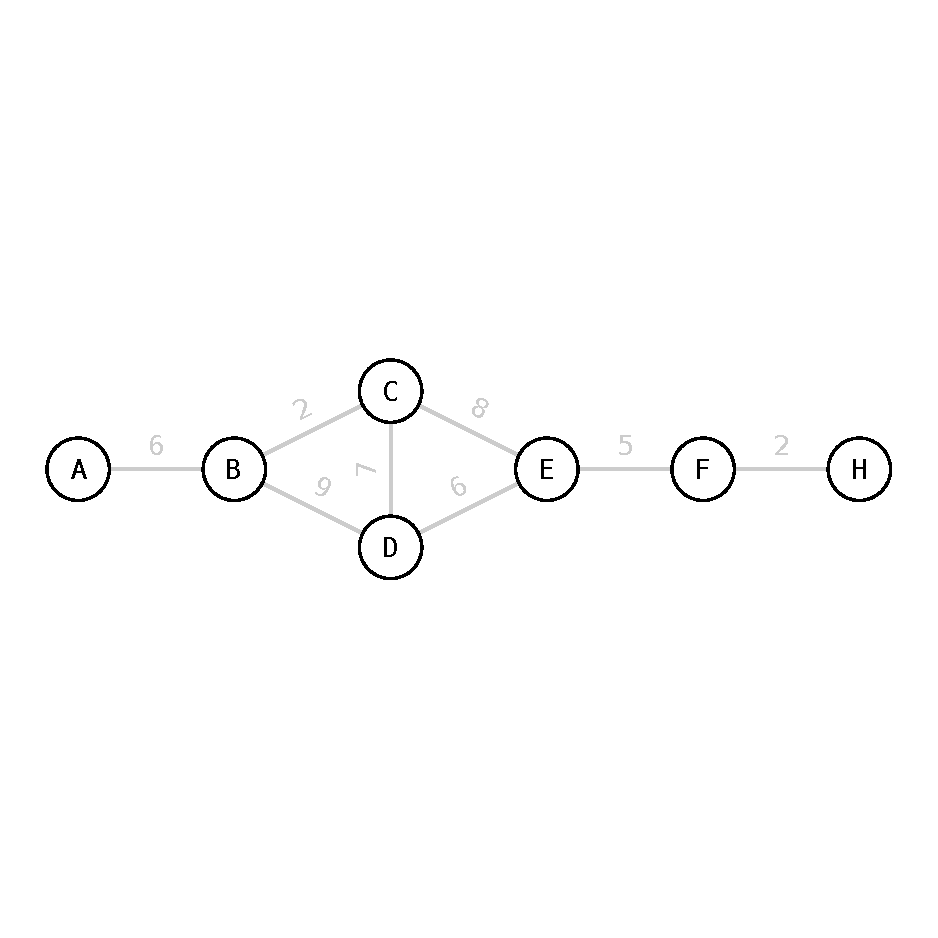
\includegraphics[width=0.28\textwidth]{python/lec13/dijkstra/dijkstra-0.pdf}\\[2pt]{\scriptsize Шаг 0}} &
\shortstack{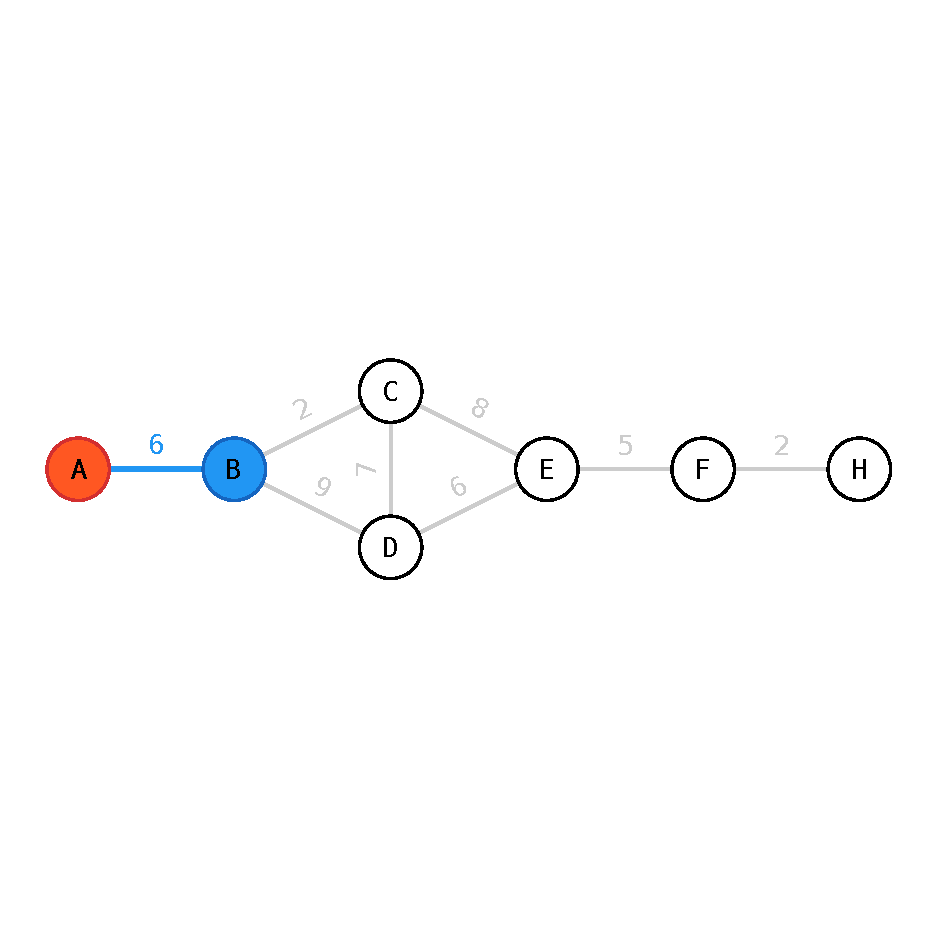
\includegraphics[width=0.28\textwidth]{python/lec13/dijkstra/dijkstra-1.pdf}\\[2pt]{\scriptsize Шаг 1}} &
\shortstack{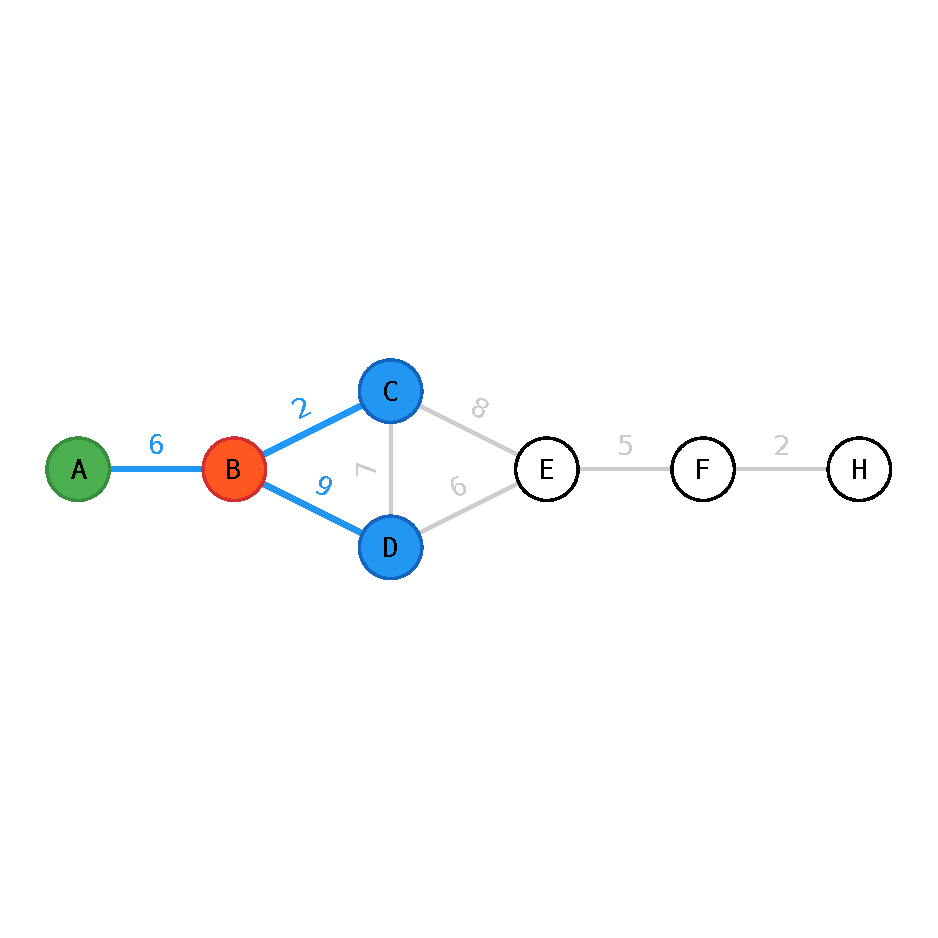
\includegraphics[width=0.28\textwidth]{python/lec13/dijkstra/dijkstra-2.pdf}\\[2pt]{\scriptsize Шаг 2}} \\
\end{tabular}\end{center}
\begin{center}\begin{tabular}{ccc}
\shortstack{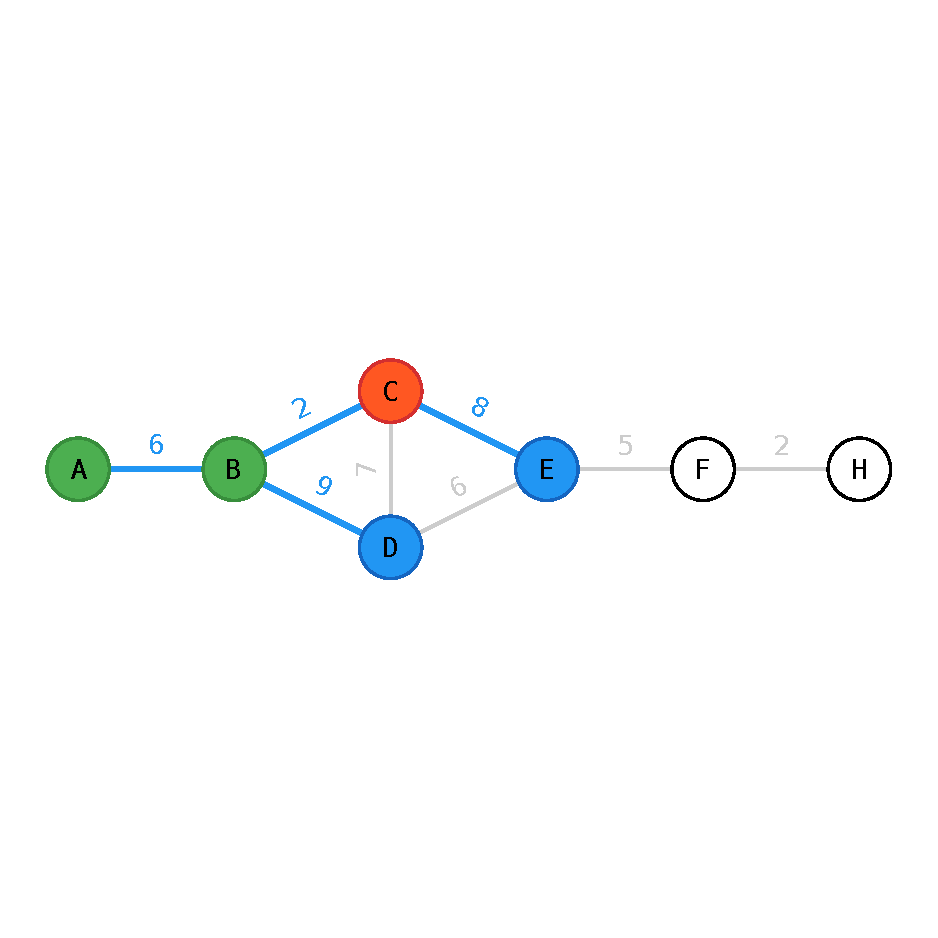
\includegraphics[width=0.28\textwidth]{python/lec13/dijkstra/dijkstra-3.pdf}\\[2pt]{\scriptsize Шаг 3}} &
\shortstack{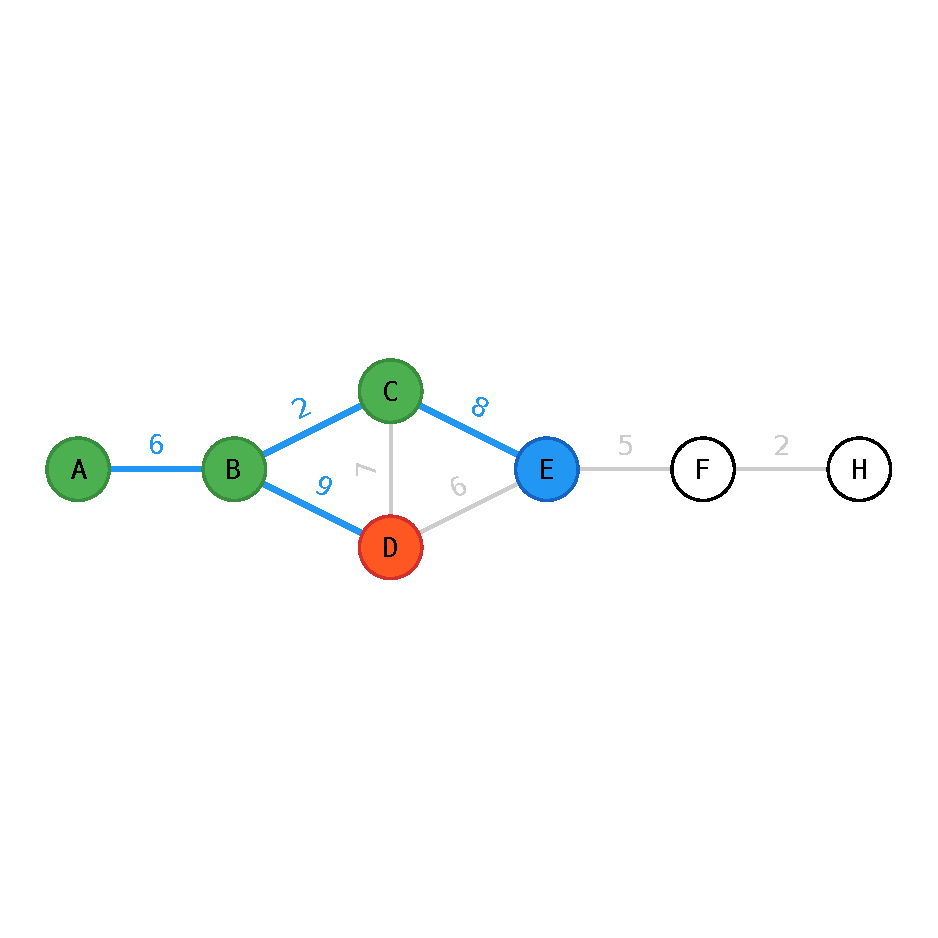
\includegraphics[width=0.28\textwidth]{python/lec13/dijkstra/dijkstra-4.pdf}\\[2pt]{\scriptsize Шаг 4}} &
\shortstack{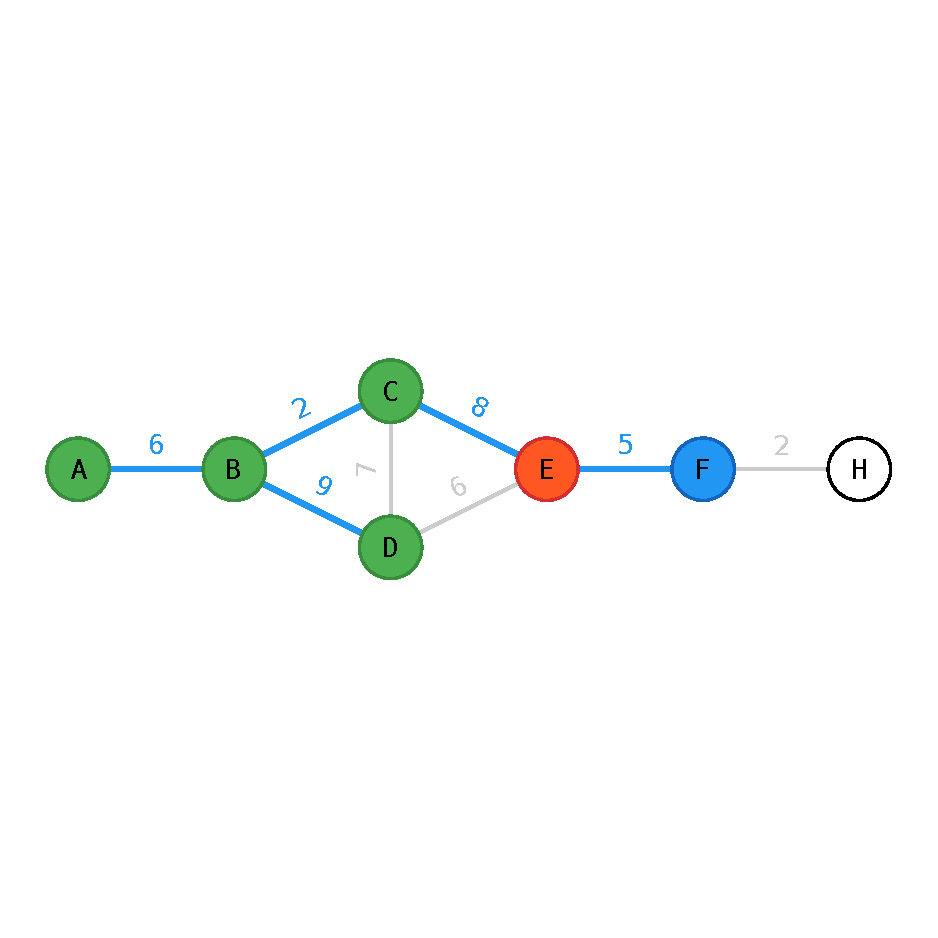
\includegraphics[width=0.28\textwidth]{python/lec13/dijkstra/dijkstra-5.pdf}\\[2pt]{\scriptsize Шаг 5}} \\
\end{tabular}\end{center}
\begin{center}\begin{tabular}{ccc}
\shortstack{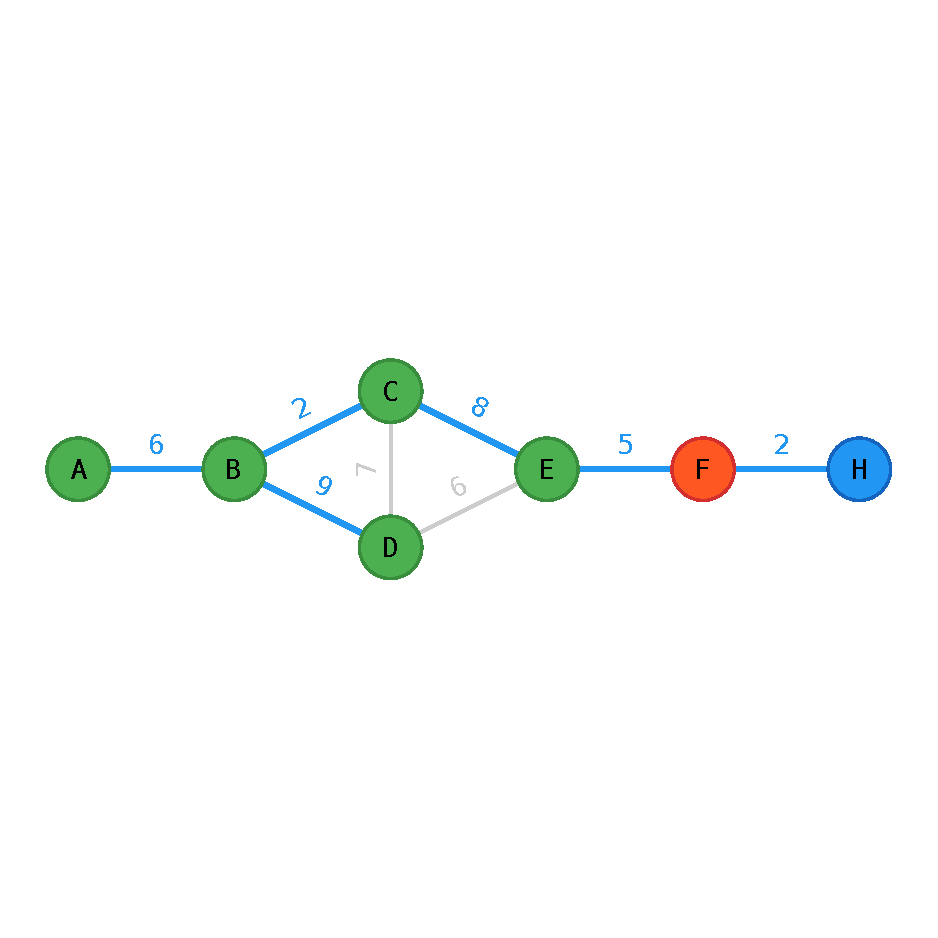
\includegraphics[width=0.28\textwidth]{python/lec13/dijkstra/dijkstra-6.pdf}\\[2pt]{\scriptsize Шаг 6}} &
\shortstack{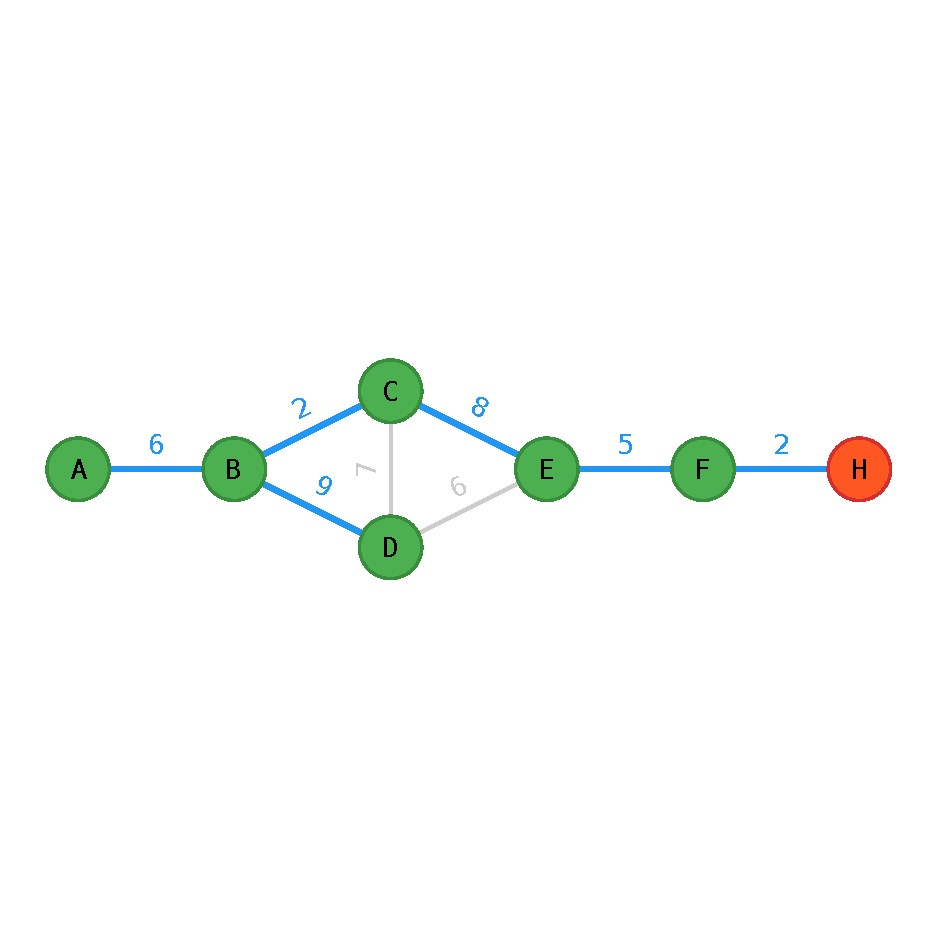
\includegraphics[width=0.28\textwidth]{python/lec13/dijkstra/dijkstra-7.pdf}\\[2pt]{\scriptsize Шаг 7}} &
\shortstack{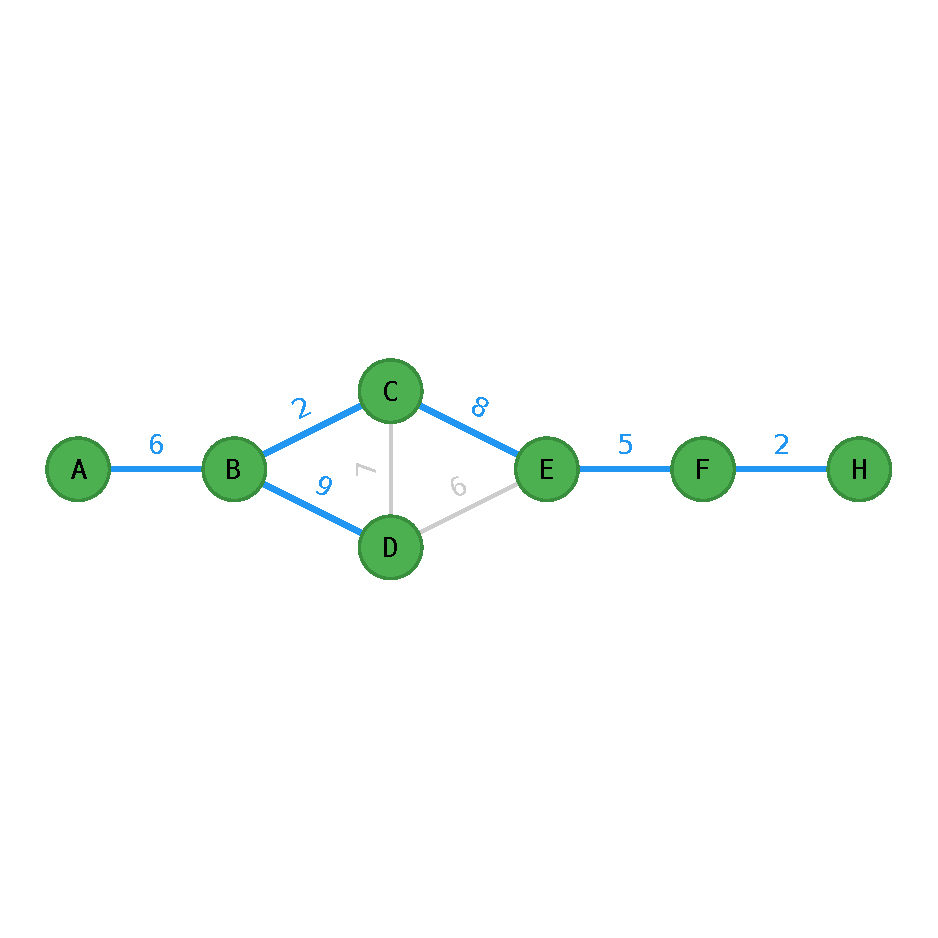
\includegraphics[width=0.28\textwidth]{python/lec13/dijkstra/dijkstra-8.pdf}\\[2pt]{\scriptsize Шаг 8}} \\
\end{tabular}\end{center}

\end{algo}

% ===========================================================
%  Алгоритм Форда-Беллмана
% ===========================================================

\begin{algo}{Алгоритм Форда-Беллмана}{ford-bellman}

\textbf{Допускается:} $\sigma\colon E \to \mathbb{R}$ (в том числе отрицательные веса).

\textbf{Инициализация:}
Произвольное упорядочивание рёбер. Стартовая вершина $v$: $\mu(v) := 0$, $\mu(w) := \infty$ для остальных.

\textbf{Шаг} (1 шаг = полный просмотр списка рёбер):

$\forall\, e_i \in \mathrm{list}(E)$, $e_i = uv$:
\[
  \text{если } \mu(v) > \mu(u) + \sigma(e_i), \text{ то }
  \begin{cases}
    \mu(v) := \mu(u) + \sigma(e_i), \\
    P(v) := u.
  \end{cases}
\]

\textbf{Конец алгоритма:} шаги $k$ и $k+1$ дают одинаковый результат. Если $n$ вершин, то алгоритм сойдётся не позже чем за $n - 1$ шагов.

\textit{Почему работает:} индукцией по $k$ проверяется инвариант ---
после $k$-го прохода по списку рёбер метка $\mu(w)$ не превосходит длины
кратчайшего пути из старта в $w$, содержащего $\le k$ рёбер (релаксация
последнего ребра такого пути произойдёт не позже $k$-го прохода).
Кратчайшие пути просты, т.\,е.\ содержат не более $n - 1$ ребра, поэтому
$n - 1$ проходов достаточно. Если же обновления случаются и на $n$-м
проходе --- в графе есть достижимый отрицательный цикл (так его и
детектируют).

\textbf{Пример} (рис.~p30-fb-example-1): граф $A, B, C, D$. Start $= B$. Отличие от Дейкстры: ребро $BA$ имеет вес $-2$.

\grfig{figures/p30-fb-example-1.pdf}{Алг. Форда-Беллмана: тот же граф, BA=-2}

Список рёбер с весами:
\begin{center}
\begin{tabular}{cc}
Ребро & Вес \\
\hline
$AC$ & 10 \\
$AD$ & 2 \\
$BA$ & $-2$ \\
$BD$ & 7 \\
$CB$ & 5 \\
$DC$ & 3 \\
\end{tabular}
\end{center}

Протокол:
\begin{center}
\begin{tabular}{c|c|c|c|c}
       & $A$    & $B$ & $C$                & $D$    \\
\hline
Иниц.  & $\infty$ & 0 & $\infty$          & $\infty$ \\
Шаг 1  & $-2, B$  & 0 & $7+3=10, D$       & $7, B$   \\
Шаг 2  & $-2, B$  & 0 & $8, A$ $\to$ $3, D$ & $0, A$   \\
\end{tabular}
\end{center}

Корневое дерево кратчайших путей: $B \xrightarrow{-2} A \xrightarrow{2} D \xrightarrow{3} C$.

\medskip
\noindent\textbf{Работа алгоритма по шагам:}
\begin{center}\begin{tabular}{ccc}
\shortstack{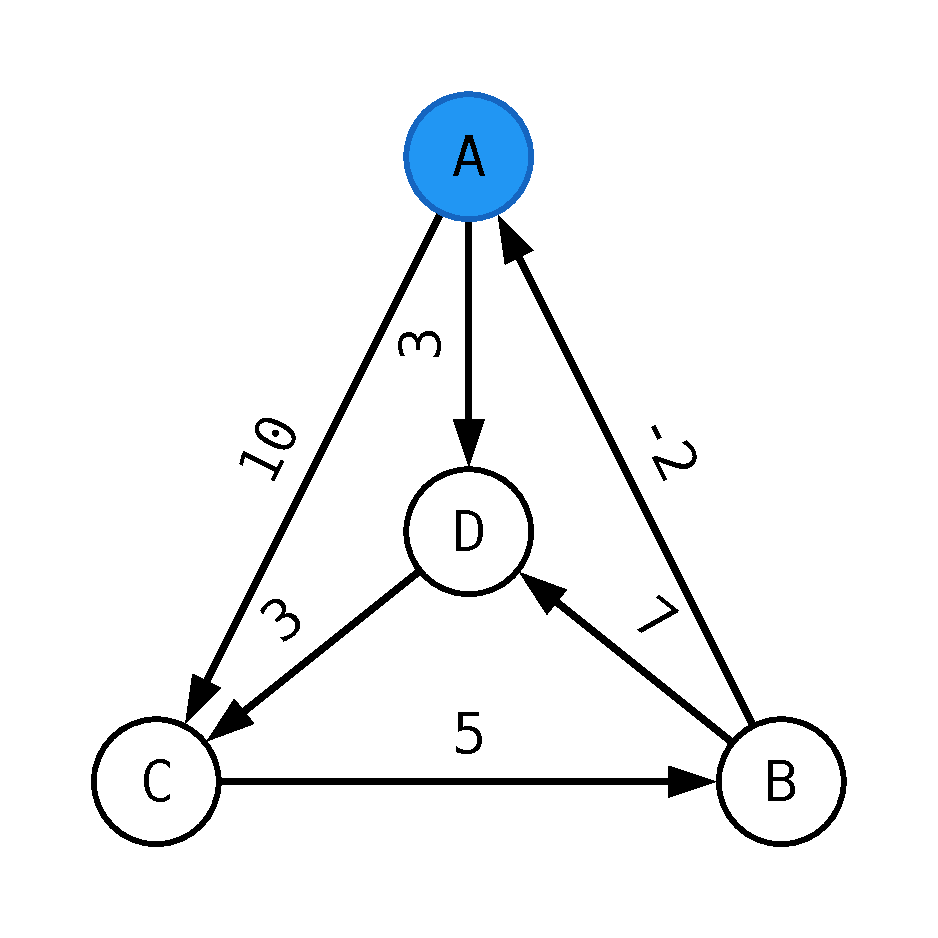
\includegraphics[width=0.28\textwidth]{python/lec13/bellman_ford/bellman_ford-0.pdf}\\[2pt]{\scriptsize Шаг 0}} &
\shortstack{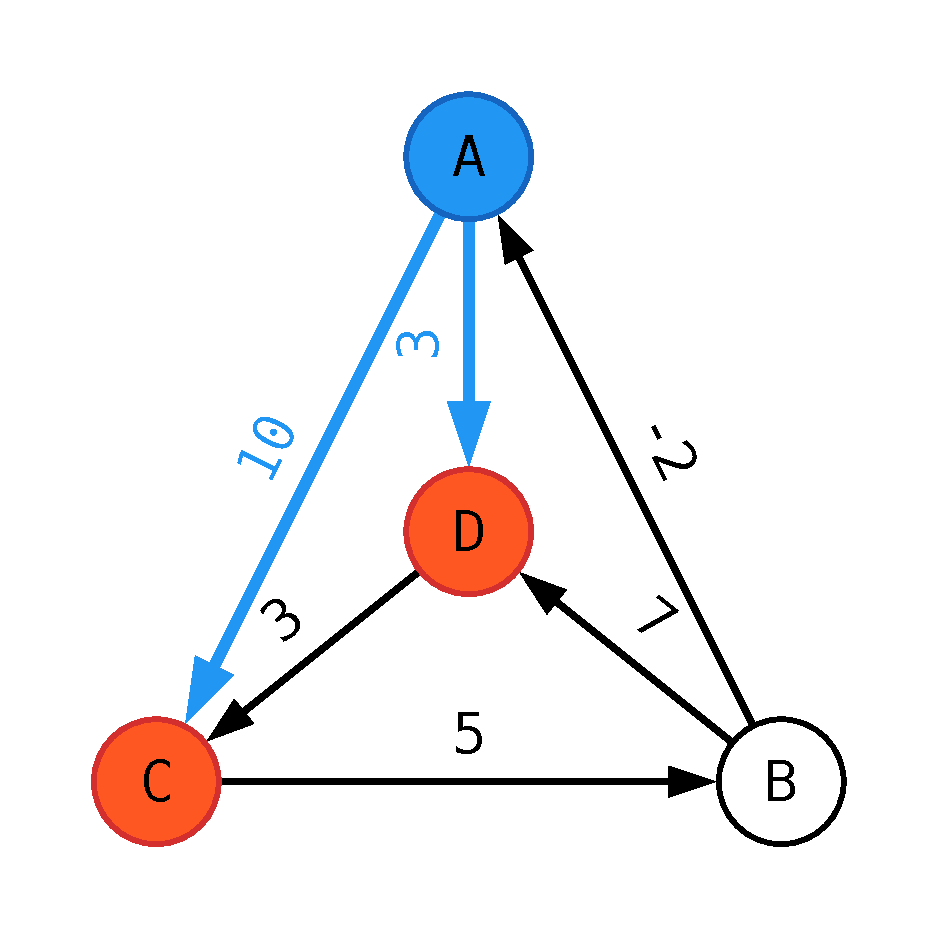
\includegraphics[width=0.28\textwidth]{python/lec13/bellman_ford/bellman_ford-1.pdf}\\[2pt]{\scriptsize Шаг 1}} &
\shortstack{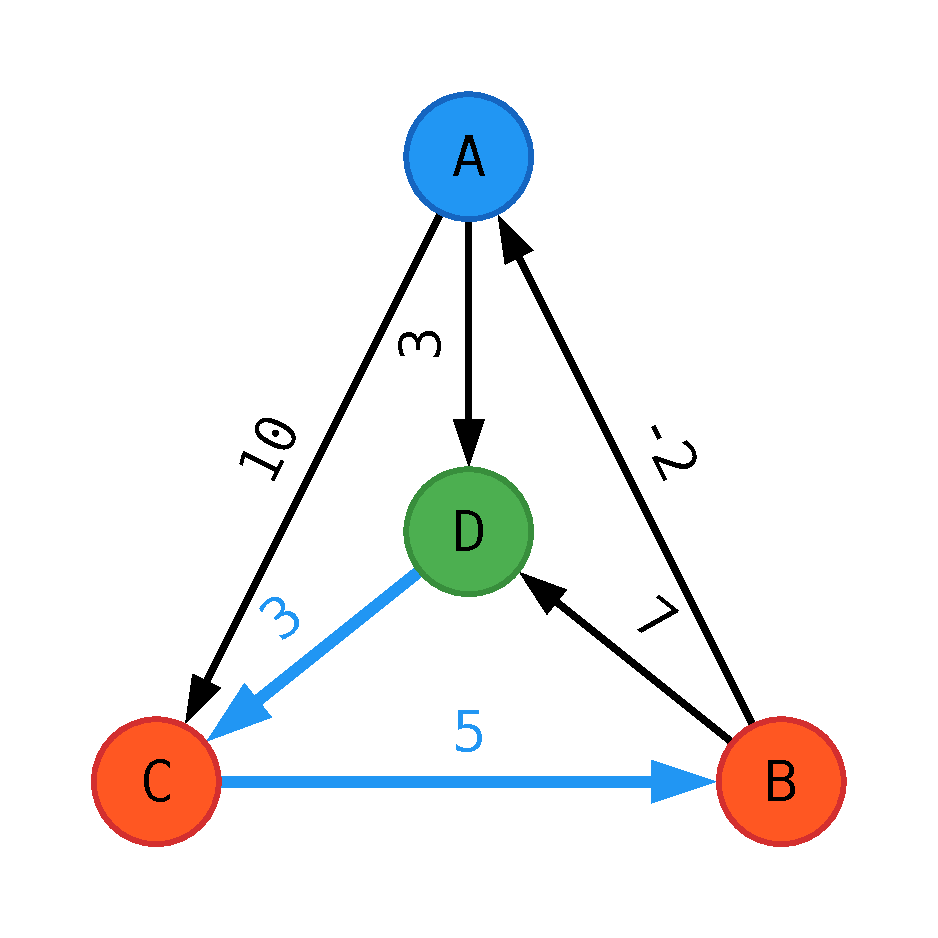
\includegraphics[width=0.28\textwidth]{python/lec13/bellman_ford/bellman_ford-2.pdf}\\[2pt]{\scriptsize Шаг 2}} \\
\end{tabular}\end{center}
\begin{center}\begin{tabular}{cc}
\shortstack{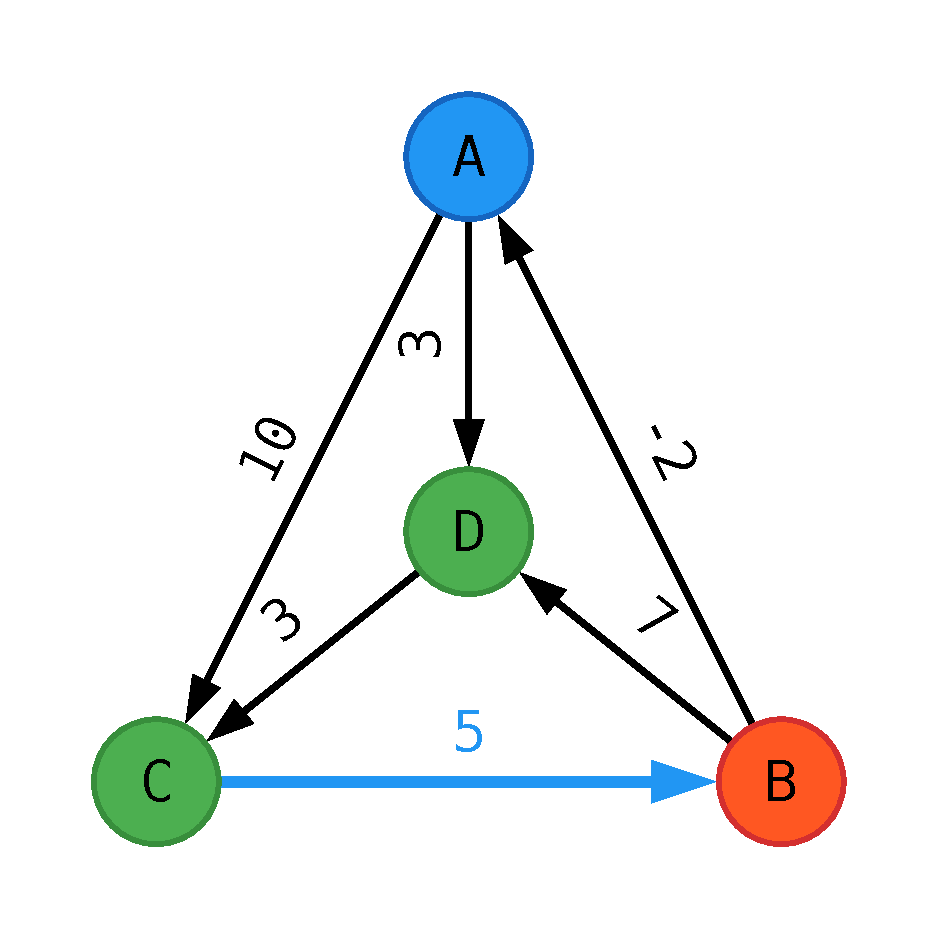
\includegraphics[width=0.28\textwidth]{python/lec13/bellman_ford/bellman_ford-3.pdf}\\[2pt]{\scriptsize Шаг 3}} &
\shortstack{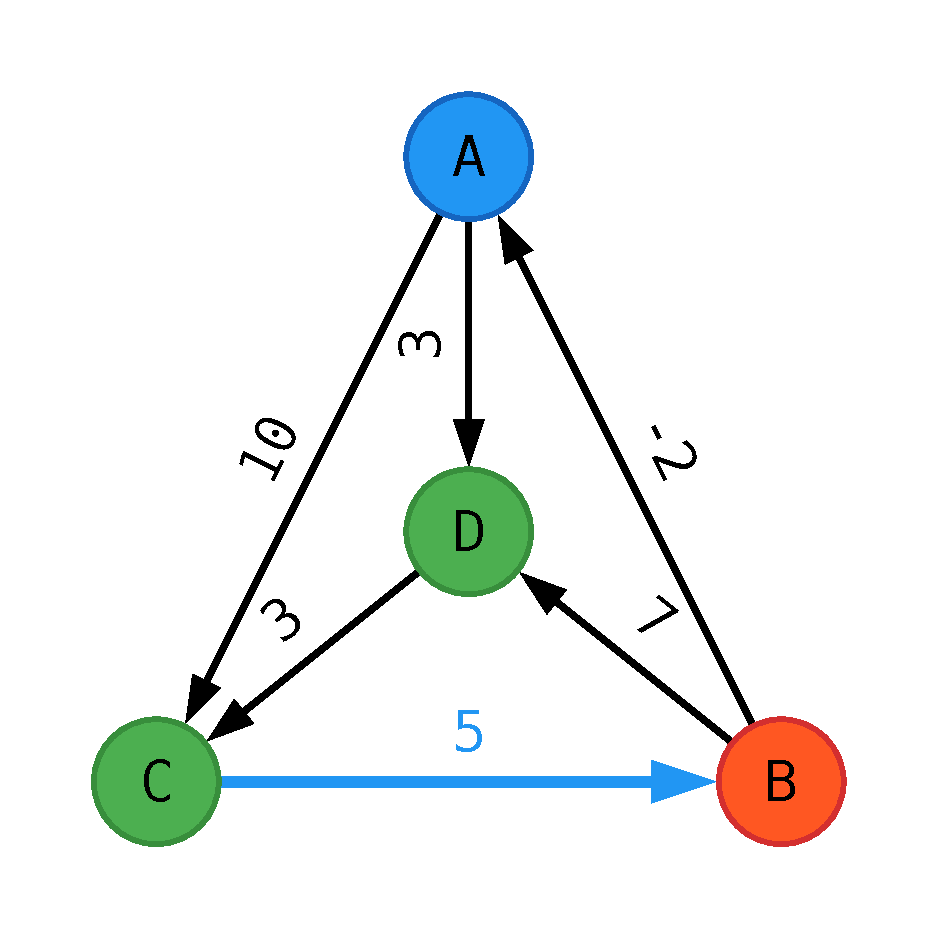
\includegraphics[width=0.28\textwidth]{python/lec13/bellman_ford/bellman_ford-4.pdf}\\[2pt]{\scriptsize Шаг 4}} \\
\end{tabular}\end{center}

\end{algo}

% ===========================================================
%  Алгоритм Флойда-Уоршелла
% ===========================================================

\begin{algo}{Алгоритм Флойда-Уоршелла}{floyd-warshall}

\textbf{Задача} $\odot$: кратчайшие пути для каждой пары $u, v \in V$.

\textbf{Идея:} аналог алгоритма Уоршелла (транзитивное замыкание), но для взвешенного графа.

\textbf{Инициализация:} Матрица $\mu(u, w)$~--- по весам рёбер. Диагональ: $\mu(v,v) = 0$. Нет ребра: $\mu(u,w) = \infty$.

\textbf{Шаг:} $v$~--- ведущая вершина. На $i$-м шаге выделяем $i$-ю строку и $i$-й столбец и смотрим пересечения:

$\forall\, (u, w)$, где $u \neq v$, $w \neq v$:
\[
  \text{если } \mu(u, w) > \mu(u, v) + \mu(v, w), \text{ то }
  \begin{cases}
    \mu(u, w) := \mu(u, v) + \mu(v, w), \\
    P(w) :=
    \begin{cases}
      v, & \text{если } P(v) = \varnothing, \\
      P(v), & \text{если } P(v) \neq \varnothing.
    \end{cases}
  \end{cases}
\]

\textbf{Пример} (рис.~p31-fu-example-1): тот же граф $A, B, C, D$.

\grfig{figures/p31-fu-example-1.pdf}{Алг. Флойда-Уоршелла: тот же граф (BA=-2)}

Шаг~0 (инициализация):
\begin{center}
\begin{tabular}{c|cccc}
     & $A$      & $B$      & $C$      & $D$      \\
\hline
$A$  & 0        & $\infty$ & 10       & 2        \\
$B$  & $-2$     & 0        & $\infty$ & 7        \\
$C$  & $\infty$ & 5        & 0        & $\infty$ \\
$D$  & $\infty$ & $\infty$ & 3        & 0        \\
\end{tabular}
\end{center}

Шаг~1 (ведущая $A$): $\mu(B,C)\colon \infty > (-2)+10 = 8\,(A)$; $\mu(B,D)\colon 7 > (-2)+2 = 0\,(A)$.
\begin{center}
\begin{tabular}{c|cccc}
     & $A$      & $B$      & $C$      & $D$      \\
\hline
$A$  & 0        & $\infty$ & 10       & 2        \\
$B$  & $-2$     & 0        & $8, A$   & $0, A$   \\
$C$  & $\infty$ & 5        & 0        & $\infty$ \\
$D$  & $\infty$ & $\infty$ & 3        & 0        \\
\end{tabular}
\end{center}

Шаг~2 (ведущая $B$): $\mu(C,A)\colon \infty > 5+(-2) = 3\,(B)$; $\mu(C,D)\colon \infty > 5+0 = 5\,(B)$.
\begin{center}
\begin{tabular}{c|cccc}
     & $A$      & $B$      & $C$      & $D$      \\
\hline
$A$  & 0        & $\infty$ & 10       & 2        \\
$B$  & $-2$     & 0        & $8, A$   & $0, A$   \\
$C$  & $3, B$   & 5        & 0        & $5, B$   \\
$D$  & $\infty$ & $\infty$ & 3        & 0        \\
\end{tabular}
\end{center}

Шаг~3 (ведущая $C$): $\mu(A,B)\colon \infty > 10+5 = 15\,(C)$; $\mu(D,A)\colon \infty > 3+3 = 6\,(C)$; $\mu(D,B)\colon \infty > 3+5 = 8\,(C)$.
\begin{center}
\begin{tabular}{c|cccc}
     & $A$      & $B$      & $C$      & $D$      \\
\hline
$A$  & 0        & $15, C$  & 10       & 2        \\
$B$  & $-2$     & 0        & $8, A$   & $0, A$   \\
$C$  & $3, B$   & 5        & 0        & $5, B$   \\
$D$  & $6, C$   & $8, C$   & 3        & 0        \\
\end{tabular}
\end{center}

Шаг~4 (ведущая $D$): $\mu(A,B)\colon 15 > 2 + 8 = 10\,(D)$ --- путь $A \to D \to C \to B$; $\mu(A,C)\colon 10 > 2+3 = 5\,(D)$; $\mu(B,C)\colon 8 > 0+3 = 3\,(A)$ --- путь $B \to A \to D \to C$, первая путевая точка $A$.
\begin{center}
\begin{tabular}{c|cccc}
     & $A$      & $B$      & $C$      & $D$      \\
\hline
$A$  & 0        & $10, D$  & $5, D$   & 2        \\
$B$  & $-2$     & 0        & $3, A$   & $0, A$   \\
$C$  & $3, B$   & 5        & 0        & $5, B$   \\
$D$  & $6, C$   & $8, C$   & 3        & 0        \\
\end{tabular}
\end{center}

\textbf{Восстановление:}
$A \to D$: путевая точка не записана (прямое ребро), путь $A \to D$,
длина $= 2$.
$C \to B$: путевая точка тоже не записана --- кратчайший путь так и
остался прямым ребром $C \to B$ длины $5$ (обходы $C \to A \to \ldots$
дороже: $\mu(C,A) = 3$, а ребра $A \to B$ нет, $\mu(A,B) = 10$).
$A \to B$: $P_{AB} = D$, далее $\mu(D, B)$: $P_{DB} = C$, далее прямое
ребро $C \to B$; итог $A \xrightarrow{2} D \xrightarrow{3} C
\xrightarrow{5} B$, длина $= 10$.

\textbf{Циклы отрицательного суммарного веса} $\Leftrightarrow$ отрицательные значения на главной диагонали.

\end{algo}

% ============================================================
\begin{task}{Кратчайшие пути: алгоритм Дейкстры}{dijkstra-task}
\textbf{Условие.} Дан неориентированный взвешенный граф на вершинах
$S,A,B,C,D,F$ с рёбрами
\[
  SA=2,\ SB=5,\ AB=1,\ AC=4,\ BD=3,\ CD=1,\ CF=6,\ DF=2.
\]
Найдите кратчайшие расстояния от вершины $S$ до всех остальных алгоритмом Дейкстры.

\smallskip
\grfig[0.42]{python/03-dijkstra/3-dijkstra-0.pdf}{Граф задачи (условие)}

\textbf{Решение.} Дейкстра поддерживает множество вершин с окончательно
найденным расстоянием. На каждом шаге фиксируется вершина с наименьшей текущей
оценкой $d$, после чего релаксируются её рёбра.
\begin{enumerate}
  \item Старт: $d[S]=0$, остальные $=\infty$. Фиксируем $S$:
        $d[A]=2,\ d[B]=5$.
  \item Минимум среди нефиксированных --- $A\,(2)$. Фиксируем $A$:
        $d[B]=\min(5,\,2+1)=3$, $d[C]=2+4=6$.
  \item Минимум --- $B\,(3)$. Фиксируем $B$: $d[D]=3+3=6$.
  \item Минимум --- $C\,(6)$. Фиксируем $C$: $D$ ($6+1=7>6$ --- без изменений),
        $d[F]=6+6=12$.
  \item Минимум --- $D\,(6)$. Фиксируем $D$: $d[F]=\min(12,\,6+2)=8$.
  \item Фиксируем $F\,(8)$. Все вершины обработаны.
\end{enumerate}

%% [серия шагов перенесена в раздел алгоритма]

\textbf{Ответ.} $d[S]=0,\ d[A]=2,\ d[B]=3,\ d[C]=6,\ d[D]=6,\ d[F]=8$.
\end{task}

% ============================================================
\begin{task}{Кратчайшие пути с отрицательными рёбрами: Форд—Беллман}{bellman-task}
\textbf{Условие.} Дан \emph{ориентированный} взвешенный граф на вершинах
$S,A,B,C,D,F$ с дугами
\[
  S\!\to\!A=3,\ S\!\to\!B=2,\ A\!\to\!C=2,\ B\!\to\!A=-2,\
  C\!\to\!D=1,\ B\!\to\!D=5,\ D\!\to\!F=3,\ C\!\to\!F=6.
\]
Найдите кратчайшие расстояния от $S$ алгоритмом Форда—Беллмана.

\smallskip
\grfig[0.42]{python/04-bellman-ford/4-bellman-ford-0.pdf}{Граф задачи (условие)}

\textbf{Решение.} Форд—Беллман выполняет до $|V|-1$ итераций, на каждой
релаксируя все дуги; отрицательные веса допустимы (при отсутствии отрицательных
циклов).
\begin{itemize}
  \item \textbf{Итерация 1.} $d[A]=3,\ d[B]=2,\ d[C]=5$; затем дуга
        $B\!\to\!A$ улучшает $d[A]=2-2=0$; далее $d[D]=6,\ d[F]=9$.
  \item \textbf{Итерация 2.} Так как $d[A]$ упало до $0$, пересчёт даёт
        $d[C]=0+2=2$, $d[D]=2+1=3$, $d[F]=3+3=6$.
  \item \textbf{Итерация 3.} Изменений нет --- расстояния стабилизировались.
\end{itemize}
Заметим: кратчайший путь до $A$ идёт \emph{не} напрямую $S\!\to\!A$ (вес $3$),
а через $S\!\to\!B\!\to\!A$ (вес $2+(-2)=0$). Именно из-за отрицательной дуги
здесь нужен Форд—Беллман, а не Дейкстра.

%% [серия шагов перенесена в раздел алгоритма]

\textbf{Ответ.} $d[S]=0,\ d[A]=0,\ d[B]=2,\ d[C]=2,\ d[D]=3,\ d[F]=6$.
\end{task}


% ===========================================================
%  Лекция 14. Алгоритм Флойда. Алгоритм Джонсона
% ===========================================================

\chapter{Лекция 14. Алгоритм Флойда. Алгоритм Джонсона}

% ===========================================================
%  Алгоритм Флойда (подробный пример)
% ===========================================================

\begin{algo}{Алгоритм Флойда}{floyd}

$G(V, E)$~--- слабо связный ориентированный граф, $\sigma\colon E \to \mathbb{R}$.

Алгоритм аналогичен Флойду--Уоршеллу. На каждом шаге выделяем ведущую вершину (строку и столбец), проверяем все пересечения.

\textbf{Хранение пути:} для пары $(u, w)$ храним $P_{uw}$~--- первую путевую точку. Для прямого ребра $A \to B$~--- ничего хранить не надо. Остаток пути: $B \to \ldots \to L$.

Если $\mu(u,w) > \mu(u,v) + \mu(v,w)$, то $\mu(u,w) := \mu(u,v) + \mu(v,w)$, $P_{uw} := P_{uv}$ (или $v$, если $P_{uv}$ пуст).

\textbf{Пример} (рис.~p32-f-example-1): граф $A, B, C, D$.

Список рёбер с весами:
\begin{center}
\begin{tabular}{cc}
Ребро & Вес \\
\hline
$AB$ & 1 \\
$BC$ & 1 \\
$BD$ & 3 \\
$CA$ & $-2$ \\
$CD$ & 1 \\
$DA$ & 4 \\
\end{tabular}
\end{center}

\grfig[0.45]{figures/p32-f-example-1.pdf}{Алг. Флойда: $A,B,C,D$ ($AB{=}1$, $BC{=}1$, $BD{=}3$, $CA{=}-2$, $CD{=}1$, $DA{=}4$)}

Шаг~0 (инициализация):
\begin{center}
\begin{tabular}{c|cccc}
     & $A$      & $B$      & $C$      & $D$      \\
\hline
$A$  & 0        & 1        & $\infty$ & $\infty$ \\
$B$  & $\infty$ & 0        & 1        & 3        \\
$C$  & $-2$     & $\infty$ & 0        & 1        \\
$D$  & 4        & $\infty$ & $\infty$ & 0        \\
\end{tabular}
\end{center}

Шаг~1 (ведущая $A$): выделяем строку $A$ и столбец $A$. Обновления: $\mu(C,B)\colon \infty > (-2) + 1 = -1$; $\mu(D,B)\colon \infty > 4 + 1 = 5$.
\begin{center}
\begin{tabular}{c|cccc}
     & $A$      & $B$      & $C$      & $D$      \\
\hline
$A$  & 0        & 1        & $\infty$ & $\infty$ \\
$B$  & $\infty$ & 0        & 1        & 3        \\
$C$  & $-2$     & $-1, A$  & 0        & 1        \\
$D$  & 4        & $5, A$   & $\infty$ & 0        \\
\end{tabular}
\end{center}

Шаг~2 (ведущая $B$): обновления: $\mu(A,C)\colon \infty > 1 + 1 = 2$; $\mu(A,D)\colon \infty > 1 + 3 = 4$; $\mu(D,C)\colon \infty > 5 + 1 = 6$.
\begin{center}
\begin{tabular}{c|cccc}
     & $A$      & $B$      & $C$      & $D$      \\
\hline
$A$  & 0        & 1        & $2, B$   & $4, B$   \\
$B$  & $\infty$ & 0        & 1        & 3        \\
$C$  & $-2$     & $-1, A$  & 0        & 1        \\
$D$  & 4        & $5, A$   & $6, A$   & 0        \\
\end{tabular}
\end{center}

Шаг~3 (ведущая $C$): обновления: $\mu(A,D)\colon 4 > 2 + 1 = 3$; $\mu(B,A)\colon \infty > 1 + (-2) = -1$; $\mu(B,D)\colon 3 > 1 + 1 = 2$.
\begin{center}
\begin{tabular}{c|cccc}
     & $A$      & $B$      & $C$      & $D$      \\
\hline
$A$  & 0        & 1        & $2, B$   & $3, B$   \\
$B$  & $-1, C$  & 0        & 1        & $2, C$   \\
$C$  & $-2$     & $-1, A$  & 0        & 1        \\
$D$  & 4        & $5, A$   & $6, A$   & 0        \\
\end{tabular}
\end{center}

Шаг~4 (ведущая $D$): нет изменений (все пути через $D$ дороже найденных).
\begin{center}
\begin{tabular}{c|cccc}
     & $A$      & $B$      & $C$      & $D$      \\
\hline
$A$  & 0        & 1        & $2, B$   & $3, B$   \\
$B$  & $-1, C$  & 0        & 1        & $2, C$   \\
$C$  & $-2$     & $-1, A$  & 0        & 1        \\
$D$  & 4        & $5, A$   & $6, A$   & 0        \\
\end{tabular}
\end{center}

\medskip
\noindent\textbf{Работа алгоритма по шагам.} Ведущая вершина ---
оранжевая; найденные на текущем шаге кратчайшие обходы --- зелёные дуги
с новой длиной, найденные ранее --- светло-фиолетовые:

\begin{center}\begin{tabular}{ccc}
\shortstack{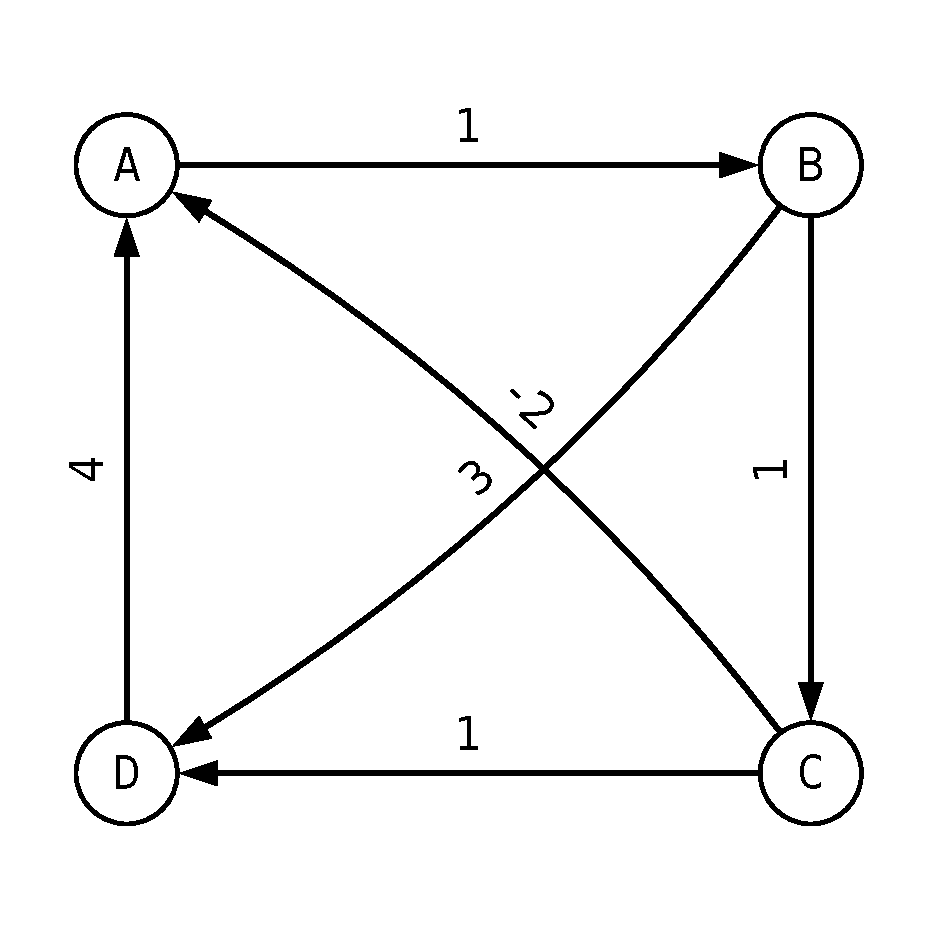
\includegraphics[width=0.30\textwidth]{python/lec14/floyd/floyd-0.pdf}\\[2pt]{\scriptsize Шаг 0. Исходный граф}} &
\shortstack{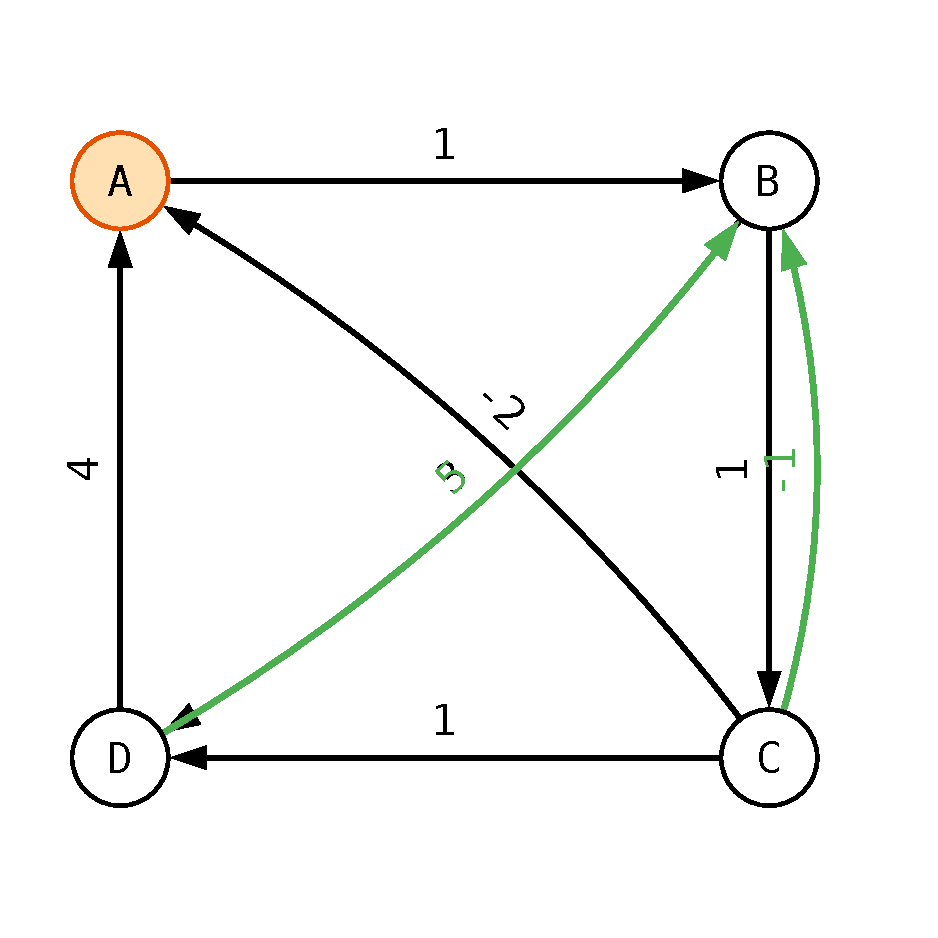
\includegraphics[width=0.30\textwidth]{python/lec14/floyd/floyd-1.pdf}\\[2pt]{\scriptsize Шаг 1. Через $A$: $CB{=}{-}1$, $DB{=}5$}} &
\shortstack{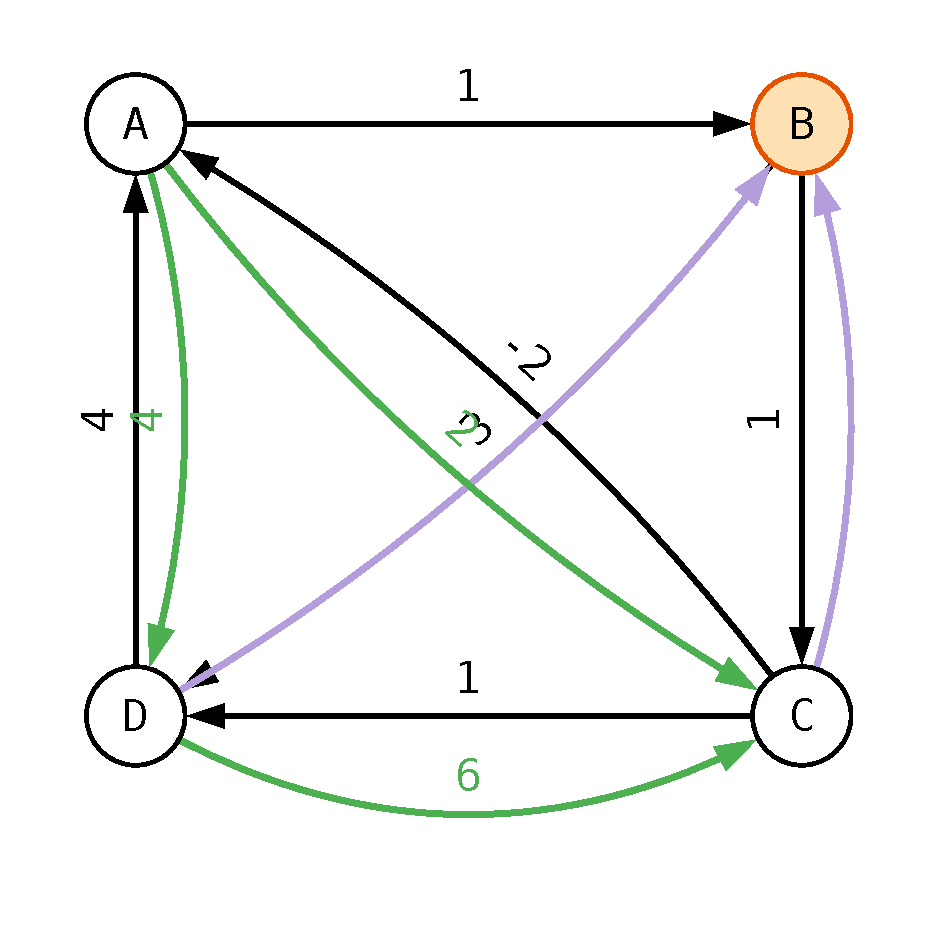
\includegraphics[width=0.30\textwidth]{python/lec14/floyd/floyd-2.pdf}\\[2pt]{\scriptsize Шаг 2. Через $B$: $AC{=}2$, $AD{=}4$, $DC{=}6$}} \\
\end{tabular}\end{center}
\begin{center}\begin{tabular}{cc}
\shortstack{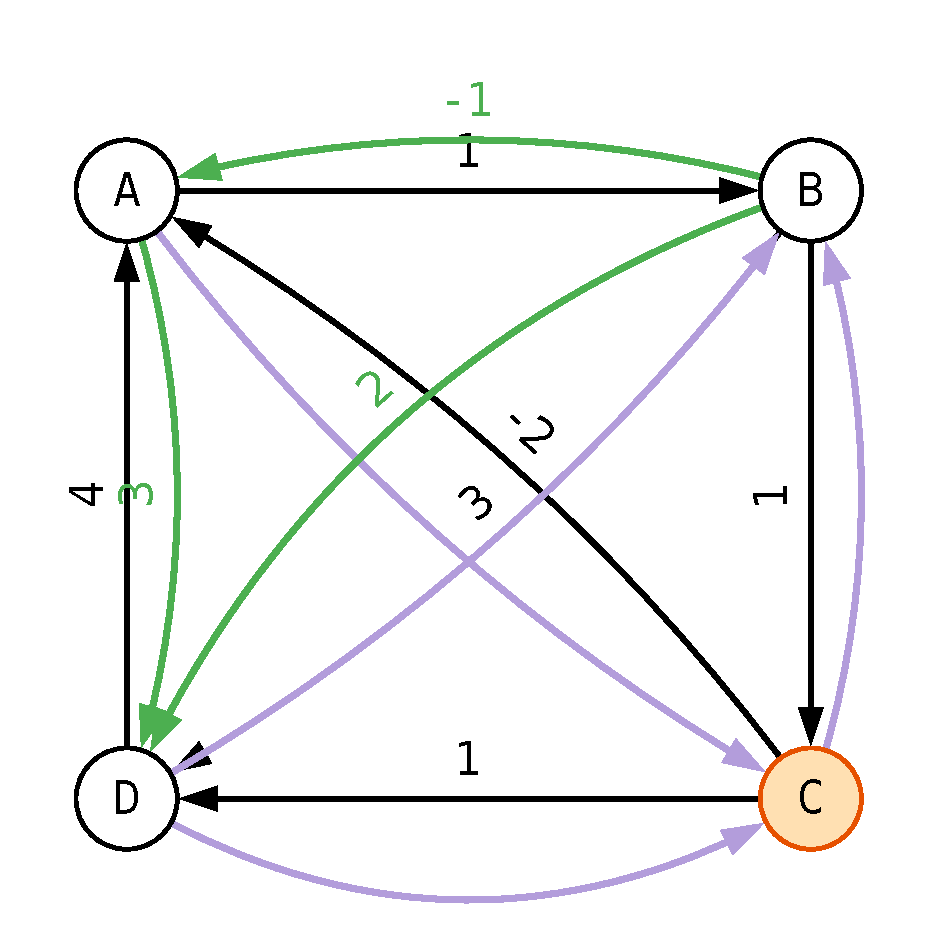
\includegraphics[width=0.30\textwidth]{python/lec14/floyd/floyd-3.pdf}\\[2pt]{\scriptsize Шаг 3. Через $C$: $AD{=}3$, $BA{=}{-}1$, $BD{=}2$}} &
\shortstack{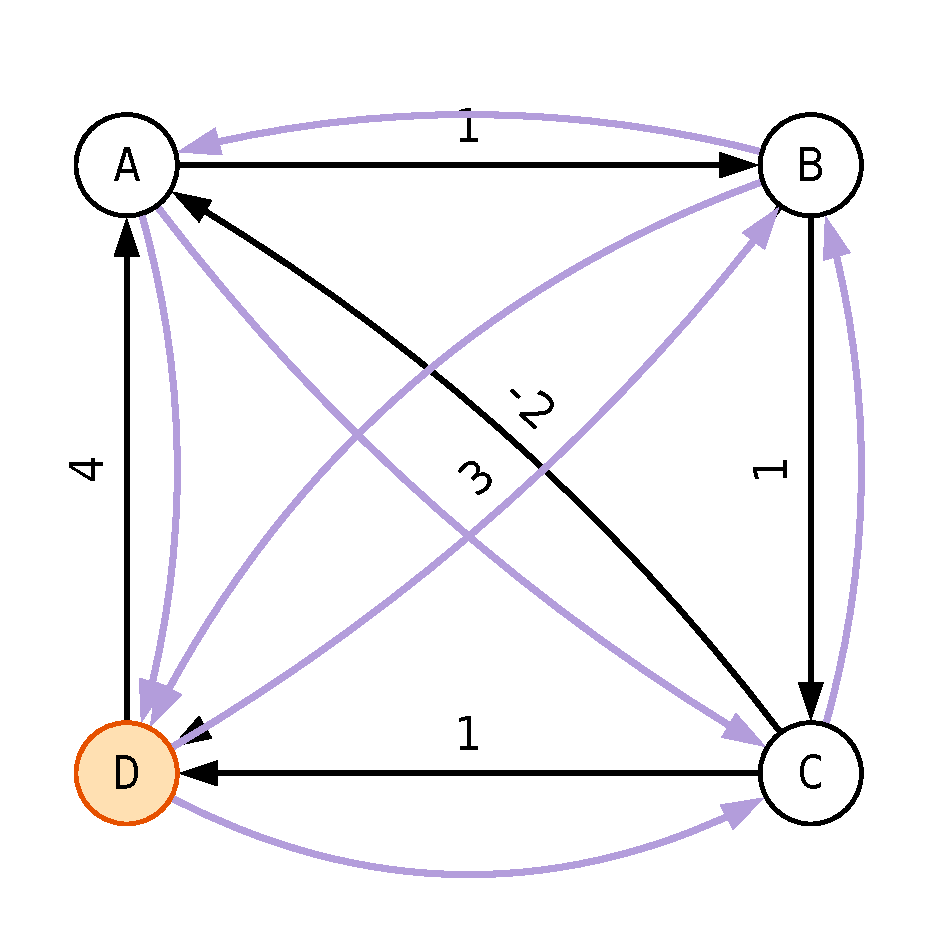
\includegraphics[width=0.30\textwidth]{python/lec14/floyd/floyd-4.pdf}\\[2pt]{\scriptsize Шаг 4. Через $D$ обновлений нет --- итог}} \\
\end{tabular}\end{center}

\textbf{Восстановление путей:}

$A \to D$: $P_{AD} = B$. $A \xrightarrow{1} B$, $P_{BD} = C$, $B \xrightarrow{1} C$, $P_{CD}$ пуст, $C \xrightarrow{1} D$. Итого: $A \xrightarrow{1} B \xrightarrow{1} C \xrightarrow{1} D$, длина $= 3$.

$C \to B$: $P_{CB} = A$. $C \xrightarrow{-2} A$, $P_{AB}$ пуст, $A \xrightarrow{1} B$. Итого: $C \xrightarrow{-2} A \xrightarrow{1} B$, длина $= -1$.

\medskip
\textbf{Циклы отрицательного суммарного веса} $\Leftrightarrow$ отрицательные значения на главной диагонали.

\textit{Почему:} диагональный элемент $\mu(v, v)$ --- длина кратчайшего
замкнутого маршрута через $v$; он станет отрицательным в точности тогда,
когда через $v$ проходит цикл отрицательного веса. Здесь диагональ
нулевая: например, цикл $A \to B \to C \to A$ весит $1 + 1 - 2 = 0$,
отрицательных циклов нет.

\end{algo}

% ===========================================================
%  Алгоритм Джонсона
% ===========================================================

\begin{algo}{Алгоритм Джонсона}{johnson}

Преобразование графа к виду с неотрицательными весами рёбер с сохранением набора кратчайших путей.

$G(V, E)$~--- слабо связный, $\sigma\colon E \to \mathbb{R}$.

\textbf{Идея.} Дейкстра быстрее Флойда ($|V|$ запусков Дейкстры дешевле
при разреженных графах), но не работает с отрицательными рёбрами.
Джонсон <<выпрямляет>> веса потенциалами так, что все веса становятся
неотрицательными, а кратчайшие пути не меняются.

\textbf{Шаг 1. Джонсоновский потенциал.}

Добавляем фиктивную вершину $S$: $\forall\, u \in V\colon e_u = Su$, $\sigma(e_u) = 0$.

\grfig[0.45]{figures/p33-jonson-example-1.pdf}{Алг. Джонсона: тот же граф + фиктивная $S$ (синие дуги веса 0)}

Запускаем \textbf{алгоритм Форда--Беллмана} от $S$ (Дейкстру пока
нельзя --- веса ещё отрицательные); $h(u) :=$ найденное расстояние от
$S$ до $u$.

Результат Форда--Беллмана (потенциалы):
\[
  h(A) = -2, \quad h(B) = -1, \quad h(C) = h(D) = 0.
\]
(Проверка: до $C$ и $D$ дешевле всего прямые нулевые дуги из $S$, т.\,е.
$h(C) = h(D) = 0$; до $A$ выгоден путь $S \to C \to A$ весом
$0 + (-2) = -2$; до $B$ --- путь $S \to C \to A \to B$ весом
$0 - 2 + 1 = -1$.)

\textbf{Шаг 2. Пересчёт весов.}

Новая весовая функция:
\[
  \tilde{\sigma}(\overline{uv}) = \sigma(\overline{uv}) + h(u) - h(v) \geq 0.
\]

\textit{Почему $\tilde\sigma \ge 0$:} $h$ --- корректные расстояния от
$S$, поэтому для любого ребра $uv$ выполнено неравенство треугольника
$h(v) \le h(u) + \sigma(uv)$, что и означает
$\sigma(uv) + h(u) - h(v) \ge 0$.

\begin{center}
\begin{tabular}{c|c|c|l}
Ребро & $\sigma$ & $\tilde{\sigma}$ & Вычисление \\
\hline
$AB$ & 1 & 0 & $1 + (-2) - (-1) = 0$ \\
$BC$ & 1 & 0 & $1 + (-1) - 0 = 0$ \\
$BD$ & 3 & 2 & $3 + (-1) - 0 = 2$ \\
$CA$ & $-2$ & 0 & $-2 + 0 - (-2) = 0$ \\
$CD$ & 1 & 1 & $1 + 0 - 0 = 1$ \\
$DA$ & 4 & 6 & $4 + 0 - (-2) = 6$ \\
\end{tabular}
\end{center}

\grfig[0.42]{figures/p33-jonson-2.pdf}{Перевешенный граф: все $\tilde\sigma \ge 0$}

Все $\tilde{\sigma} \geq 0$~--- можно применять Дейкстру!

\textbf{Шаг 3. Дейкстра от каждой вершины} с весами $\tilde{\sigma}$.

Матрица расстояний в весах $\tilde\sigma$:
\begin{center}
\begin{tabular}{c|cccc}
$\mathrm{dist}_{\tilde\sigma}$ & $A$ & $B$ & $C$ & $D$ \\
\hline
$A$  & 0 & 0 & 0 & 1 \\
$B$  & 0 & 0 & 0 & 1 \\
$C$  & 0 & 0 & 0 & 1 \\
$D$  & 6 & 6 & 6 & 0 \\
\end{tabular}
\end{center}

(Например, из $D$: единственный выход --- дуга $DA$ веса $6$, дальше
всё бесплатно по нулевым дугам $A \to B \to C$; поэтому вся строка $D$
равна $6$.)

\textbf{Шаг 4. Обратный пересчёт.}

Для получения истинных расстояний:
\[
  \mathrm{dist}_\sigma(u,v) = \mathrm{dist}_{\tilde\sigma}(u,v) - h(u) + h(v).
\]

\textit{Почему пути не изменились:} для любого пути
$u = x_0 \to x_1 \to \ldots \to x_k = v$ его новая длина равна
\[
  \sum_i \tilde\sigma(x_i x_{i+1})
  = \sum_i \sigma(x_i x_{i+1}) + h(u) - h(v)
\]
--- телескопическая сумма: все промежуточные потенциалы сокращаются.
Все пути из $u$ в $v$ сдвинулись на \emph{одну и ту же} константу
$h(u) - h(v)$, поэтому порядок путей по длине (и сами кратчайшие пути)
сохранился, а формула пересчёта очевидна.

Итоговая матрица истинных расстояний
($\mathrm{dist}_\sigma = \mathrm{dist}_{\tilde\sigma} - h(u) + h(v)$):
\begin{center}
\begin{tabular}{c|cccc}
$\mathrm{dist}_{\sigma}$ & $A$ & $B$ & $C$ & $D$ \\
\hline
$A$  & 0    & 1    & 2 & 3 \\
$B$  & $-1$ & 0    & 1 & 2 \\
$C$  & $-2$ & $-1$ & 0 & 1 \\
$D$  & 4    & 5    & 6 & 0 \\
\end{tabular}
\end{center}

Например, $\mathrm{dist}_\sigma(D, A) = 6 - h(D) + h(A) = 6 - 0 - 2 = 4$;
$\mathrm{dist}_\sigma(B, A) = 0 - (-1) + (-2) = -1$. Матрица совпала с
результатом алгоритма Флойда выше --- проверка пройдена. $\checkmark$

\textbf{Свойства:}
\begin{enumerate}
  \item Набор кратчайших путей для $G$ в терминах $\sigma$ и $\tilde{\sigma}$ совпадает (пути не меняются, только длины) --- телескопическая сумма выше.
  \item $\forall\, e \in E\colon \tilde{\sigma}(e) \geq 0$ (неравенство треугольника для корректных потенциалов).
  \item Если $\tilde{\sigma}(e) < 0$ для какого-то ребра~--- значит, потенциалы найдены неправильно.
\end{enumerate}

\end{algo}

% ============================================================
\begin{task}{Кратчайшие пути между всеми парами: алгоритм Флойда}{floyd-task}
\textbf{Условие.} Дан ориентированный взвешенный граф на вершинах $A,B,C,D$ с
дугами
\[
  A\!\to\!B=3,\ A\!\to\!C=8,\ B\!\to\!C=2,\ B\!\to\!D=5,\ C\!\to\!D=1,\ D\!\to\!A=2.
\]
Найдите кратчайшие расстояния между всеми парами вершин алгоритмом Флойда.

\begin{center}
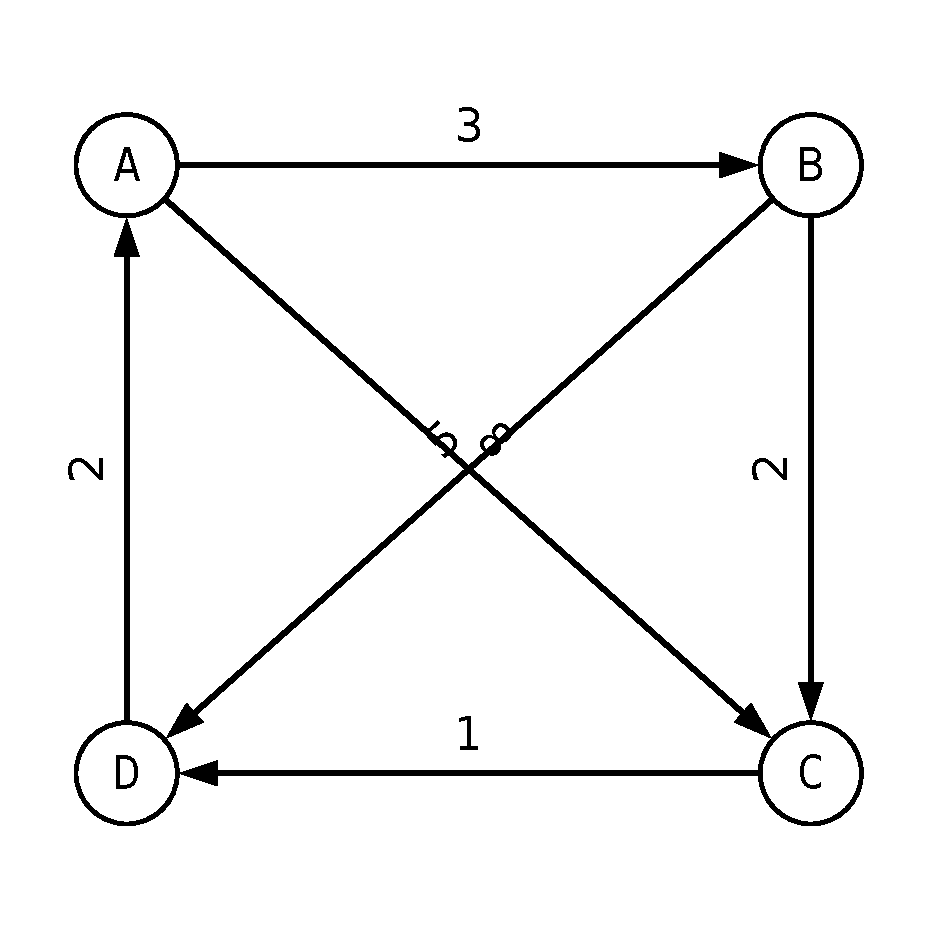
\includegraphics[width=0.42\textwidth]{figures/task-floyd-1.pdf}
\end{center}

\smallskip
\textbf{Решение.} Флойд последовательно разрешает в качестве промежуточных
вершины $A,B,C,D$. На шаге $k$ обновляем
$d[i][j]\leftarrow\min\bigl(d[i][j],\,d[i][k]+d[k][j]\bigr)$.

Начальная матрица $D^{(0)}$ (на диагонали $0$, отсутствующие дуги --- $\infty$):
\begin{center}
\renewcommand{\arraystretch}{1.25}
\begin{tabular}{|c||c|c|c|c|}
\hline
$D^{(0)}$ & \textbf{A} & \textbf{B} & \textbf{C} & \textbf{D} \\ \hline\hline
\textbf{A} & 0 & 3 & 8 & $\infty$ \\ \hline
\textbf{B} & $\infty$ & 0 & 2 & 5 \\ \hline
\textbf{C} & $\infty$ & $\infty$ & 0 & 1 \\ \hline
\textbf{D} & 2 & $\infty$ & $\infty$ & 0 \\ \hline
\end{tabular}
\end{center}

\noindent\textbf{Через $A$:} обновляются пути из $D$ ($D\!\to\!A=2$):
$D\!\to\!B=2+3=5$, $D\!\to\!C=2+8=10$.

\noindent\textbf{Через $B$:} $A\!\to\!C=\min(8,3+2)=5$, $A\!\to\!D=3+5=8$;
$D\!\to\!C=\min(10,5+2)=7$.

\noindent\textbf{Через $C$:} $A\!\to\!D=\min(8,5+1)=6$, $B\!\to\!D=\min(5,2+1)=3$.

\noindent\textbf{Через $D$:} замыкаются обратные пути:
$B\!\to\!A=3+2=5$, $C\!\to\!A=1+2=3$, $C\!\to\!B=1+2+3=6$ и т.\,д.

Итоговая матрица кратчайших расстояний $D^{(4)}$:
\begin{center}
\renewcommand{\arraystretch}{1.25}
\begin{tabular}{|c||c|c|c|c|}
\hline
$D^{(4)}$ & \textbf{A} & \textbf{B} & \textbf{C} & \textbf{D} \\ \hline\hline
\textbf{A} & 0 & 3 & 5 & 6 \\ \hline
\textbf{B} & 5 & 0 & 2 & 3 \\ \hline
\textbf{C} & 3 & 6 & 0 & 1 \\ \hline
\textbf{D} & 2 & 5 & 7 & 0 \\ \hline
\end{tabular}
\end{center}

Проверка: $B\!\to\!A$ идёт по маршруту $B\!\to\!C\!\to\!D\!\to\!A=2+1+2=5$;
$C\!\to\!B=C\!\to\!D\!\to\!A\!\to\!B=1+2+3=6$ --- совпадает с таблицей.

\textbf{Ответ.} Матрица кратчайших расстояний $D^{(4)}$ приведена выше.
\end{task}



% =============================================================================
% СБОРНИКИ
% =============================================================================

\appendix

\chapter*{Все определения}
\addcontentsline{toc}{chapter}{Все определения}
\printdefinitionsummary

\chapter*{Все теоремы и утверждения}
\addcontentsline{toc}{chapter}{Все теоремы и утверждения}
\printtheoremsummary

\chapter*{Все алгоритмы}
\addcontentsline{toc}{chapter}{Все алгоритмы}
\printalgorithmsummary

\chapter*{Все задачи}
\addcontentsline{toc}{chapter}{Все задачи}
\printtasksummary

\end{document}
